\documentclass[11pt,          % font size: 11pt or 12pt
               phd,           % degree:    ms or phd
               onehalfspacing % spacing: onehalfspacing or doublespacing
               ]{ncsuthesis}

%%----------------------------------------------------------------------------%%
%%------------------------------ Import Packages -----------------------------%%
%%----------------------------------------------------------------------------%%

\usepackage{booktabs}  % professionally typeset tables
\usepackage{amsmath}%,amssymb,amsfonts}
\usepackage{textcomp}  % better copyright sign, among other things
%\usepackage{xcolor}
\usepackage{lipsum}    % filler text
%\usepackage{subfig}    % composite figures

%%ORTIZ PACKAGES

%%----------------------------------------------------------------------------%%
%%--------------------------- Personal Packages ------------------------------%%
%%----------------------------------------------------------------------------%%

%\usepackage{comment}
%\usepackage{algorithm,algorithmic}
\usepackage{algorithmic}
\usepackage[ruled, vlined, linesnumbered]{algorithm2e}
\usepackage{tabularx}
\usepackage{multirow}
\usepackage[list=true,justification=centering]{subcaption}
%\usepackage[format=plain,justification=RaggedRight,singlelinecheck=true,font=large,labelfont=bf,labelsep=space]{caption}
\usepackage[format=plain,justification=justified,singlelinecheck=true,font=large,labelfont=bf,labelsep=space]{caption} 
\usepackage{adjustbox}
\usepackage{mfirstuc}
\usepackage{xspace}
\usepackage{enumitem,kantlipsum}
\usepackage{grffile}
\usepackage{pbox}
\usepackage{pifont}% http://ctan.org/pkg/pifont
\newcommand{\cmark}{\ding{51}}%
\newcommand{\xmark}{\ding{55}}%

%%%%%%%%%%%%%%%%%%%%%%%%%%%%%%%%%%%%%%%%%%
%%%%%%%%%%% Old bibliography commands
%%%%%%%%%%%%%%%%%%%%%%%%%%%%%%%%%%%%%%%%%%5
%\usepackage[super,sort&compress,comma,square,authoryear]{natbib} %\cite command %Added by Ortiz

%use the following line with plainnat
%\usepackage[super,sort&compress,comma,square,numbers]{natbib} %\cite command %Added by Ortiz
%\usepackage{natbib}

%\usepackage[style=alphabetic,natbib=true,backend=bibtex
%sorting=nyt,firstinits=true,isbn=false,doi=false,url=false]{biblatex} %couldn't get backend=biber to work

%\usepackage{filecontents}

%\bibliography{Ortiz-thesis2}
%\bibliographystyle{plain}


%%%%%%%%%%%%%%%%%%%%%%%%%%%%%%%%%%%%%%%%%%
%%%%%%%%%%% Hack for alphanumeric bibliography
%%%%%%%%%%%%%%%%%%%%%%%%%%%%%%%%%%%%%%%%%%5
\RequirePackage[
			style=numeric-comp,%alphabetic,%numeric-comp,%authoryear-comp,%
			sorting=nyt,%ynt					
			hyperref=true, %	
			firstinits=true,%
			backend=bibtex,
			natbib=true,
			url=false,
			isbn=false,
			maxnames=2, %for et al to be used
			maxalphanames=1, %to avoid printing a + for every et al in the abbreviation
			doi=false]{biblatex}		
			

%needed to do et al after two names
%http://tex.stackexchange.com/questions/44048/use-et-al-in-biblatex-custom-style
\renewcommand*{\finalnamedelim}{\addspace\&\space}

%Simplify abbreviation (the default uses either one or two authors and it indicates et al with a +)
%The following five lines make it so that only the first author is used in the abbreviation
%http://tex.stackexchange.com/questions/27956/label-only-from-first-author
\renewcommand*{\labelalphaothers}{}
    \renewcommand*{\intitlepunct}{}
    \DefineBibliographyStrings{german}{in={}}
    \DefineBibliographyStrings{english}{in={}}
    \DeclareNameAlias{sortname}{last-first}
    \DeclareNameAlias{default}{last-first}
	
%\AtEveryCitekey{\ifciteseen{}{\defcounter{maxnames}{99}}} %authoryear			
\DeclareFieldFormat[article,periodical]{volume}{\mkbibbold{#1}}
\makeatletter

\newrobustcmd*{\parentexttrack}[1]{%
  \begingroup
  \blx@blxinit
  \blx@setsfcodes
  \blx@bibopenparen#1\blx@bibcloseparen
  \endgroup}

\AtEveryCite{%
  \let\parentext=\parentexttrack%
  \let\bibopenparen=\bibopenbracket%
  \let\bibcloseparen=\bibclosebracket}

\makeatother
\renewcommand{\cite}[1]{\parencite{#1}}


\renewbibmacro{in:}{%
  \ifentrytype{article}{}{%
  \printtext{\bibstring{in}\intitlepunct}}}
  
\AtEveryBibitem{\clearfield{month}}

\AtEveryBibitem{\clearfield{language}}
%%%%%%%%%%%%%%%%%%%%%%%%%%%%%%%%%%%%%%%%%%%%%

%\addbibresource{Ortiz-thesis2.bib}
%\addbibresource{Ortiz-thesisURL.bib}
\addbibresource{thesis.bib}
\addbibresource{conference.bib}

 \defbibheading{myheading}[REFERENCES]{
 \chapter*{#1}
 %\centerline{\bf{#1}}
 \markboth{#1}{#1}}

%\usepackage{amsmath,amssymb,amsfonts} %amssymb and amsfonts cannot be used in conjunction with mdput
%\usepackage{graphicx,subfig}% Include figure files
\usepackage{dcolumn}% Align table columns on decimal point
\usepackage{bm}% bold math
%\usepackage{hyperref}% add hypertext capabilities
%\usepackage{hypernat}% make hyperref and natbib work together
\usepackage{cancel}
\usepackage{verbatim}% multiline commenting
\usepackage{ifthen}
\usepackage{url}
\urlstyle{same}
\usepackage{sectsty}
\usepackage{balance} 
%\usepackage{caption}
\usepackage{graphicx} %eps figures can be used instead
\usepackage{lastpage}
\usepackage{fancyhdr}
\pagestyle{fancy}

%http://tex.stackexchange.com/questions/100817/error-when-using-bc-from-abbrevs-in-caption
%Getting BC
\usepackage{abbrevs}
\usepackage{etoolbox}
\robustify{\DateMark} % after having loaded abbrevs

\usepackage{units} %Needed to solve bug from citation Hydrodynamics in 21/2 dimensions
%see http://www.latex-community.org/viewtopic.php?f=5&t=989

\usepackage[sharp]{easylist} %used for brainstorming purposes 
%\usepackage{mathabx} % used for \Asterisk for convolution %conflicts with \widering

%compile on single pass
%\usepackage[backend=biber,...]{biblatex}


%%%%%%%%%%%%
%%% Hack to make chapters start on odd pages
% http://tex.stackexchange.com/questions/73591/how-to-have-a-blank-even-page-before-every-chapter
%%%%%%%%%%%%
%\newcommand{\ensureoddstart}{\checkoddpage\ifoddpage\else\newpage\mbox{}\fi}
%\newcommand{\ensureoddstart}{}


%%%Fancy tables
%http://tex.stackexchange.com/questions/94032/fancy-tables-in-latex
\usepackage[table]{xcolor}
\usepackage{array,booktabs}
\usepackage{colortbl}
\newcolumntype{L}{@{}>{\kern\tabcolsep}l<{\kern\tabcolsep}}



%%%%%%%%%%
%%%%% Hack to allow more levels in outline
%%%%%%%%%%
%\setcounter{secnumdepth}{5}
%\setcounter{tocdepth}{5} %may violate ETD
%Usage http://pleasemakeanote.blogspot.com/2010/06/how-to-activate-subsubsubsection-in.html
%\section{} % level 1
%\subsection{} % level 2
%\subsubsection{} % level 3
%\paragraph{} % level 4 - equivalent to subsubsubsection
%\subparagraph{} % level 5

%http://tex.stackexchange.com/questions/60209/how-to-add-an-extra-level-of-sections-with-headings-below-subsubsection
\usepackage{titlesec}

\setcounter{secnumdepth}{4}

\titleformat{\paragraph}
{\normalfont\normalsize\bfseries}{\theparagraph}{1em}{}
\titlespacing*{\paragraph}
{0pt}{3.25ex plus 1ex minus .2ex}{1.5ex plus .2ex}

%%%%%%%%%%%%%%%%%%%%%%%%%%
%%%% Hack for containing figures within sections
%%%%%%%%%%%%%%%%%%%%%%%%%%%%
%http://ctan.org/pkg/placeins
\usepackage{placeins}
%De�fines a \FloatBar�rier com�mand, be�yond which floats may not pass; use�ful, for ex�am�ple, to en�sure all floats for a sec�tion ap�pear be�fore the next \sec�tion com�mand.

%%%Hack for centering all figures
%\makeatletter
%\g@addto@macro\@floatboxreset\centering
%\makeatother

%%----------------------------------------------------------------------------%%
%%---------------------------- Formatting Options ----------------------------%%
%%----------------------------------------------------------------------------%%
%%

%% -------------------------------------------------------------------------- %%
%% Disposition format -- any titles, headings, section titles
%%  These formatting commands affect all headings, titles, headings,
%%  so sizing commands should not be used here.
%%  Formatting options to consider are
%%     +  \sffamily - sans serif fonts.  Dispositions are often typeset in
%%                    sans serif, so this is a good option. 
%%     +  \rmfamily - serif fonts
%%     +  \bfseries - bold face
%\dispositionformat{\sffamily\bfseries}   % bold and sans serif
\dispositionformat{\bfseries}            % bold and serif

%% -------------------------------------------------------------------------- %%
%% Formatting for centered headings - Abstract, Dedication, etc. headings
%%  This is where one might put a sizing command.
%%  \MakeUppercase can be used to typeset all headings in uppercase.
\headingformat{\large\MakeUppercase}   % All letters uppercase
%\headingformat{\large}                % Not all uppercase
%\headingformat{\Large\scshape}        % Small Caps, used with serif fonts.

%% Typographers recommend using a normal inter-word space after
%% sentences. TeX's default is to add an wider space, but \frenchspacing
%% gives a normal spacing. Comment out the following line if you prefer
%% wider spaces between sentences.
\frenchspacing


%% -------------------------------------------------------------------------- %%
%%  Optional packages
%%    A number of compatible packages to improve the look and feel of
%%    your document are available in the file optional.tex 
%%    (For example, hyperlinks, fancy chapter headings, and fonts)
%% To use these options, uncomment the next line and see optional.tex
%%  Optional Packages to consider.   These packages are compatible with
%%    ncsuthesis.  

%% -------------------------------------------------------------------------- %%
%% Fancy chapter headings
%%  available options: Sonny, Lenny, Glenn, Conny, Rejne, Bjarne
%\usepackage[Sonny]{fncychap}
%\usepackage[Rejne]{fncychap}
%\usepackage[Bjarne]{fncychap}

%%----------------------------------------------------------------------------%%
%% Hyperref package creates PDF metadata and hyperlinks in Table of Contents
%%  and citations.  Based on feedback from the NCSU thesis editor, 
%%  the links are not visually distinct from normal text (i.e. no change
%%  in color or extra boxes).
\usepackage[
  pdfauthor={Chin-Jung Hsu},
  pdftitle={Elastic Data-Intensive Computing on the Cloud},
  pdfcreator={pdftex},
  pdfsubject={NC State ETD Thesis},
  pdfkeywords={microfluidics, hard sphere, jamming, suspension, rigidity, friction, microscopy},
  colorlinks=true,
  linkcolor=black,
  citecolor=black,
  filecolor=black,
  urlcolor=black,
]{hyperref}


%% -------------------------------------------------------------------------- %%
%% Microtype - If you use pdfTeX to compile your thesis, you can use
%%              the microtype package to access advanced typographic
%%              features.  By default, using the microtype package enables
%%              character protrusion (placing glyphs a hair past the right 
%%              margin to make a visually straighter edge)
%%              and font expansion (adjusting font width slightly to get 
%%              more favorable justification).
%%              Using microtype should decrease the number of lines
%%              ending in hyphens.
\usepackage{microtype}


%%----------------------------------------------------------------------------%%
%% Fonts 

%% ETD guidelines don't specify the font.  You can enable the fonts
%%  by uncommenting the appropriate lines.  Using the default Computer 
%%  Modern fonts is *not* required.  A few common choices are below.
%%  See http://www.tug.dk/FontCatalogue/ for more options.

%% Serif Fonts -------------------------------------------------
%%  The four serif fonts listed here (Utopia, Palatino, Kerkis,
%%  and Times) all have math support.


%% Utopia
%\usepackage[T1]{fontenc}
%\usepackage[adobe-utopia]{mathdesign}

%% Palatino
%\usepackage[T1]{fontenc}
%\usepackage[sc]{mathpazo}
%\linespread{1.05}

%% Kerkis
%\usepackage[T1]{fontenc}
%\usepackage{kmath,kerkis}

%% Times
%\usepackage[T1]{fontenc}
%\usepackage{mathptmx}


%% Sans serif fonts -------------------------

%\usepackage[scaled]{helvet}  % Helvetica
%\usepackage[scaled]{berasans} % Bera Sans

%solve bug from fancyhdr in optional
%http://nw360.blogspot.com/2006/11/latex-headheight-is-too-small.html
\setlength{\headheight}{14pt}

%%----------------------------------------------------------------------------%%
%%---------------------------- Content Options -------------------------------%%
%%----------------------------------------------------------------------------%%
%% Size of committee: 3, 4, 5, or 6 -- this number includes the chair
\committeesize{4}

%% Members of committee
%%  Each of the following member commands takes an optional argument
%%   to specify their role on the committee.
%%  For co-chairs, use the commands:
%%      \cochairI{Doug Dodd}
%%      \cochairII{Chris Cox}
%%
\chair{Dr. Timothy J. Menzies}
\memberI{Dr. Kathyrn Stolee}
\memberII{Dr. Min Chi}
\memberIII{Dr. Ranga Raju Vatsavai, Ph.D. }   % unnecessary if committeesize=3
%\memberIV{Hung-Wei Tseng}    % unnecessary if committeesize=3 or 4
%\memberV{Edna Everitt}  % unnecessary if committeesize=3, 4, or 5


%% Student writing thesis, \student{First Middle}{Last}
\student{Vivek}{Nair} % a full middle name
%\student{John M.}{Smith} % a middle initial

%% Degree program
\program{Computer Science}

%% Thesis Title
%%  Keep in mind, according to ETD guidelines:
%%    +  Capitalize first letter of important words.
%%    +  Use inverted pyramid shape if title spans more than one line.
%%
%%  Note: To break the title onto multiple lines, use \break instead of \\.
%\thesistitle{A North Carolina State University Sample \LaTeX{} Thesis \break 
%with a Title So Long it Needs a Line Break}
% TODO: add verb, right now only with subject
%\thesistitle{Elastic Data-Intensive Computing for the Cloud}
\thesistitle{Frugal ways to find Good Configurations}

%% Degree year.  Necessary if your degree year doesn't equal the current year.
%\degreeyear{1995}


%%----------------------------------------------------------------------------%%
%%---------------------------- Personal Macros -------------------------------%%
%%----------------------------------------------------------------------------%%

%% A central location to add your favorite macros.

%% A few examples to get you started.
\newcommand{\uv}[1]{\ensuremath{\mathbf{\hat{#1}}}}
%\newcommand{\bo}{\ensuremath{\mathbf{\Omega}}}
\newcommand{\eref}[1]{Eq.~\ref{#1}}
\newcommand{\fref}[1]{Fig.~\ref{#1}}
\newcommand{\tref}[1]{Table~\ref{#1}}
\newcommand{\del}{\nabla}
\renewcommand{\exp}[1]{e^{#1}}
\newcommand{\Conv}{\mathop{\scalebox{1.5}{\raisebox{-0.2ex}{$\ast$}}}}%



\usepackage{color}
%\newcommand{\NEW}[1]{\textcolor{blue}{#1}}
\newcommand{\NEW}[1]{#1}
%% conflict with the algorithmc package?
%\newcommand{\COMMENT}[1]{\textcolor{green}{#1}}


\newcommand{\NOTER}[1]{\textcolor{orange}{#1}}
\newcommand{\NOTEC}[1]{\textcolor{blue}{#1}}
\newcommand{\NOTEK}[1]{\textcolor{magenta}{#1}}

\newcommand{\mum}{\ensuremath{{\mu}\text{m}}}


% customized words
% systems
\newcommand{\cat}{CAT\xspace}
\newcommand{\scout}{{\sc Scout}\xspace}
\newcommand{\insideout}{\textit{Inside-Out}\xspace}
\newcommand{\arrow}{\textit{Arrow}\xspace}
\newcommand{\micky}{\textit{Micky}\xspace}
\newcommand{\ernest}{\textit{Ernest}\xspace}
\newcommand{\cherrypick}{\textit{CherryPick}\xspace}
\newcommand{\paris}{\textit{PARIS}\xspace}
\newcommand{\bo}{Bayesian Optimization\xspace}

% words
\newcommand{\fig}[1]{Fig. #1}
\newcommand{\myfigure}[1]{Figure~#1}
\newcommand{\mytable}[1]{Table~#1}
\newcommand{\naive}{na\"ive\xspace}
\newcommand{\etal}{\textit{et al}.\xspace}
\newcommand{\ie}{\textit{i}.\textit{e}.,\xspace}
\newcommand{\eg}{\textit{e}.\textit{g}.,\xspace}
\newcommand{\etc}{\textit{etc}.\xspace}
%\newcommand{\rone}[1]{{\color{black} #1}}
%\newcommand{\rtwo}[1]{{\color{black} #1}}
\newcommand{\todo}[1]{\textbf{{\color{blue} #1}}}
\newcommand{\quotes}[1]{``#1''}
\newcommand{\myequation}[1]{Equation~#1}


%This makes it so that you can add short paths in your .tex by including the folders where you store your images in the search path
\graphicspath{
{./Chapter-Introduction/}
{./Chapter-Introduction/figures}
{./Chapter-Background/}
{./Chapter-Background/figures/}
{./Chapter-InsideOut/}
{./Chapter-InsideOut/figures/}
{./Chapter-Arrow/}
{./Chapter-Arrow/figures/}
{./Chapter-Scout/}
{./Chapter-Scout/figures/}
{./Chapter-Micky/}
{./Chapter-Micky/figures/}
{./Chapter-Trilogy/}
{./Chapter-Trilogy/figures/}
{./Chapter-DataPlacement/}
{./Chapter-DataPlacement/figures}
{./Chapter-Conclusion/}
{./Chapter-Conclusion/figures/}
}

%%---------------------------------------------------------------------------%%
\usepackage{calc}
%% Capital letter height
\newlength{\chaptercapitalheight}
\settoheight{\chaptercapitalheight}{D}
\newlength{\chapterfootskip}
\setlength{\chapterfootskip}{\chaptercapitalheight}
\addtolength{\chapterfootskip}{2\baselineskip}
\addtolength{\chapterfootskip}{0.5ex}  % A little extra space to ensure there are 2 full double spaced lines
%\def\chapterfootskipnum{\chapterfootskip}
\renewcommand{\listfigurename}{LIST OF FIGURES}
\renewcommand{\listtablename}{LIST OF TABLES}
\renewcommand{\bibname}{BIBLIOGRAPHY}

%\renewcommand{\cfttoctitlefont}{\centering\ncsu@headingformat}


%http://tex.stackexchange.com/questions/47184/height-of-figure-caption-textheight
\newlength\graphht
\newcommand\calculategraphicstargetheight[1]{%
     \setlength\graphht{\textheight 
                       -\parskip
                       -\abovecaptionskip -\belowcaptionskip
                       -(12pt * #1) % assuming baselineskip of 12pt in caption
                       -\chapterfootskip
                       }}

%\usepackage{titlesec}

%landscape support in fancyhdr from http://tex.stackexchange.com/questions/9071/how-to-translate-and-rotate-the-heading-of-landscaped-pages
\usepackage{pdflscape}
\usepackage{tikz}
\fancypagestyle{lscapedplain}{%
  \fancyhf{}
  \fancyfoot{%
    \tikz[remember picture,overlay]
      \node[outer sep=1cm,above,rotate=90] at (current page.east) {\thepage};}
\renewcommand{\headrulewidth}{0pt} 
\renewcommand{\footrulewidth}{0pt}
}

%\includeonly{front}
%\includeonly{Chapter-1/main}
                      
\begin{document}
\pagestyle{plain}
%%---------------------------------------------------------------------------%%
\frontmatter

%% ------------------------------ Abstract ---------------------------------- %%
\begin{abstract}
Most software systems available today are configurable, which gives the users an option to customize the system to achieve different functional or non-functional (better performance) properties. As systems evolve, more configuration options are added to the
software system, which leaves considerable
optimization potential untapped and induces major economic cost.
To solve this problem of finding the (near) optimal configurations,
engineers have proposed various techniques. Most popular among
them are model-based techniques, where accurate models of the configuration space are created using as few configuration measurements as possible. Previously, Guo et al. and Sarkar et al. asserted that one way to find good configurations is build very accurate model of the configuration space. However, we notice two major problems with the model-based techniques: 1) previous techniques are expensive to be practically viable, and 2) there are software systems whose configuration spaces cannot be accurately modeled. 
% Consequently, there is
% a gap between proposed techniques and practical viability of these
% techniques.
This dissertation focuses on proposing techniques which are
easier to understand and are practically viable. 

First, we present \textbf{WHAT} that exploits
some lower dimensional knowledge to build performance models. 
% Prior work on predicting the performance of software configurations suffered from either (a) requiring far too many sample configurations or (b) large variances in their predictions.Both these problems can be avoided using the \textbf{WHAT} spectral learner. 
WHAT\textquotesingle s innovation
is the use of the spectrum (eigenvalues) of the distance matrix between the
configurations of a configurable software system, to perform dimensionality reduction.
Within that reduced configuration space, many closely associated configurations
can be studied by executing only a few sample configurations. For the subject systems
studied here, a few dozen samples yield accurate and stable predictors less than
10 \% prediction error, with a standard deviation of less than 2\%. When compared
to the state of the art, WHAT (a) requires 2 to 10 times fewer samples to achieve
similar prediction accuracies, and (b) its predictions are more stable (i.e., have lower
standard deviation). 

While useful in the test domain, we found a significant drawback when exploring newer software systems. We found that the distance function used to generate the distance matrix changes with different software systems (since some configuration options have more influence on the performance than others). To overcome this,a rank-based method is proposed
which shows how an accurate model is not required for performance optimization, but a rank-preserving model is sufficient. We evaluate rank-based method with 21 scenarios based on nine software systems and demonstrate that our approach is beneficial in 16 scenarios; for the remaining five scenarios, an accurate model
can be built by using very few samples anyway, without the need
for a rank-based approach. Additionally, in 8/21 of the scenarios,
the number of measurements required by the rank-based method
is an order of magnitude smaller than methods used in prior work.

To further reduce the cost we present \textbf{FLASH},  a sequential model-based method, which sequentially explores the configuration space by reflecting on the configurations evaluated so far to determine the next best configuration to explore. FLASH scales up to software systems that defeat the prior state of the art model-based methods in this area and can solve both single-objective and multi-objective optimization problems. We evaluate FLASH using 30 scenarios based on 7 software systems to demonstrate that FLASH saves effort in 100\% and 80\% of cases in single-objective and multi-objective problems respectively by up to several orders of magnitude compared to the state of the art techniques.

Based on the above findings, we found that the previously held belief: `` highly accurate model is required to optimize software system" is an overkill and expensive. To overcome the limitation of prior works, we have explored various alternate methods to shows how a near optimal solution can be found using much fewer resources and effort. Additionally, we observed that the prior work transformed the problem of finding an optimal solution to a modelling problem---which, in our opinion, was the main roadblock to build cheaper solutions. The central insight for all the frugal alternatives (as presented in this thesis) is to solve the optimization problem and not a modelling problem. Given the success of these frugal alternatives to find good configurations, we encourage practitioners to embrace and explore similar techniques prescribed in this thesis to (a) find better configurations and (b) not to be deterred with the cost of optimizing systems. Please note, this techniques presented in this thesis are very general in nature and could potentially be used in other domains (such as Cloud Computing, Software Engineering, etc.), where the cost of collecting samples is exorbitantly high. FLASH, for instance, has already been applied to domains like Cloud Architectural Tuning, Effort Estimation and software optimization problems. We recommend that future work explores options which consumes fewer resource, which is more suitable for real world scenario. In our opinion , some suggestions are: (a) explore cheaper models, and (b) use the models to guide explorations.
\end{abstract}


%% ---------------------------- Copyright page ------------------------------ %%
%% Comment the next line if you don't want the copyright page included.
\makecopyrightpage

%% -------------------------------- Title page ------------------------------ %%
\maketitlepage

%% -------------------------------- Dedication ------------------------------ %%
\begin{dedication}
%\centering{
\begin{center}
To Ammayi---for timely advice and support
\end{center}

\end{dedication}

%% -------------------------------- Biography ------------------------------- %%
\begin{biography}
Vivek Nair was born and raised in the city of Kolkata, India. He graduate from West Bengal University of Technology and National Institute of Technology, Durgapur with and Bachelors in Technology and Master in Technology respectively. 
 His primary research interest is search based software engineering with a primary goal to solve search problems to maximize the quality of the search while minimizing the cost of search.  His current research investigated problems in the software engineering domain and developed techniques not only to solve software configuration problem, but also software product lines as well as cloud architecture tuning problems.  Before joining the PhD program, he
was a software engineer at Samsung Software Engineering Labs. 
During his PhD program, his internship experiences include LexisNexis Risk Solutions (2015-2017), and
Microsoft Research - Redmond, USA (Summer 2018). 
% He is a student member of IEEE.


\end{biography}

%% ----------------------------- Acknowledgements --------------------------- %%
\begin{acknowledgements}
\textit{*This acknowledgment contains plenty of subtexts and would be found as text within brackets. The subtext is meant to serve the purpose of comic relief and comic relief only.} \\

This thesis is no way an individual work. It is a product of a lot of love and sacrifice, tears and sweat of not just me but for various individuals who have taught lessons throughout my journey as a graduate student, here at NCSU. This text below is no way a comprehensive list of all the people who have touched my life [for better or for worse], but it has been a useful experience. 

One of the primary reasons, I can write this thesis is because of Dr. George N. Rouskas and my aunt, Dr. Latha Unni. 
My first year at NCSU was tumultuous and eventful. As new graduate student, dealing with the stresses of graduate school and the toxic environment of my previous lab was overwhelming. This resulted in me deciding to quit graduate school---which I have been so excited to attend. Dr. Rouskas, who provided me with financial support while transitioning from my old advisor to my current advisor. Both of them counseled and provided support when I required it the most. This thesis would have never been possible without these two amazing people. 

Secondly my thesis advisor [my academic father], Dr. Menzies---he is a legend [faking the Aussie accent]. He has been very [not so] patient with me and directed me towards
areas which held promise. He helped me understand the value of collaboration and being a voracious reader of the literature. 
That said I have never had a more dramatic relationship with anyone---which in retrospect was an effective way of training graduate student. Our story has all the elements of a soap opera---there are love and respect,  not so much love [hate sounds just too strong] and doubt. Either way, he played a massive part in making this thesis possible and made me a better researcher [hopefully]. 

Thirdly, I would then like to thank my dissertation committee members,
Dr. Ranga Raju Vatsavai, Dr. Min Chi and Dr. Kathryn T. Stolee,
for their valuable feedback and insight on my dissertation.

I am also grateful to my research collaborators: Sven Apel (University of Passau), Norbert Siegmund (Bauhaus-University Weimar), and Pooyan Jamshidi (University of South Carolina).  I would like to gratefully acknowledge researchers who generously shared their research tools and results used in my dissertation.  I am very much
thankful to all my peers at the RAISE Lab, for their constant support, insightful discussions and useful feedback on
my research. Dr. Wei Fu, Dr. Chin-Jung Hsu, Rahul Krishna, George Mathew [also my room-mate], and Zhe Yu for the insightful and exciting conversations [interestingly I was able to write papers with all these amazing individuals---so all our discussions were not completely useless]. 
I thank my internship mentors in the industry, who have immensely helped me expand
my research to a broader scope: Dan Camper and Arjuna Chala (Lexisnexis Risk Solutions), and Chris Duvarney, Kim Herzig, and Hitesh Sajnani (Microsoft Research, USA). 


Heartfelt thanks go to Kathy Luca, Carol Allen, and all the helpful staff at the Department
of Computer Science. I thank Amruthkiran Hedge, Anand Gorthi, Sandesh Saokar, Siddartha Chauhan, Mayank Vaish, Akhilesh Tanneru [Mr. T], and George Mathew for
sharing the apartment and making my stay at Raleigh eventful. Special thanks to Karen Warmbein, Blue and [Z]Simba whose love and support helped me survive the grind of Ph.D.



Finally, last but not least, I am very thankful to my family. My family was my constant source of support and encouragement throughout my journey as a doctoral student. 
My Ph.D. journey would not have gone so far, without you.
\end{acknowledgements}


\thesistableofcontents

\thesislistoftables

\thesislistoffigures


%%---------------------------------------------------------------------------%%
\mainmatter



\pagestyle{plain}
%\newgeometry{margin=1in,lmargin=1.25in,footskip=\chapterfootskip, includehead, includefoot}
\chapter{Introduction}
\label{chapter:one}


Modern software systems provide configuration options to modify
both functional behavior of the system (functionality of the system) and non-functional properties of the system ( performance and memory
consumption). 
Configuration options of a software system that are relevant to users are usually referred to as
\textit{features}. All the features of a system (vector of configuration options) together defines a \textit{configuration} of a software system. The features can  take integer, decimal or string values.  An important non-functional properties is performance, because it  influences  how a user interacts with the system. 
Environmental/external factors can affect performance. For example, the performance of the software system can be better for more number of cores and greater RAM memory.  A software system is required to select and set configuration options to maximize the performance of that system. For example, say we have a software system with 10 (binary) configuration options---it results in a configuration space of size $2^{10}$ or $1024$. The user of the software system, now has to find the optimal configuration for the given task (or input) in hand. 
This problem can be tackled in two different ways: (1) exhaustively measuring performance of all possible configurations---which means running 1024 benchmark runs, and (2) use domain knowledge (assuming the user has tuned similar software system before) to find the best configuration. 
However, as the number of configuration options increase, it
becomes difficult for humans to keep track of the interactions between the configuration options. This means as the configuration space grows it is harder to either exhaustively measure performance for all possible configurations or find domain experts to confidently do so. Please note that the optimal configuration can change dramatically with different inputs (tasks) and the environment---which make domain knowledge based decision less reliable. 

This exact problem has been reported by numerous researchers from different domains.
\begin{itemize}
\item Many software systems have poorly chosen defaults [1], [2]. Hence, it is useful to seek better configurations.
\item Understanding the configuration space of software systems with large configuration spaces is challenging [3].
\item Exploring more than just a handful of configurations is usually infeasible due to long benchmarking time [4].
\end{itemize}


The problem we are trying to tackle throughout this document is: ``How can we find a set of configuration options which would \underline{maximize} the performance of a system while \underline{minimizing} the cost of search''. Here were would limit our scope of study to just the configurations options or features of a particular software system (and not its environment). While exploring the above mentioned, we produced three methods:
\begin{enumerate}
    \item The paper titled ``Faster Discovery of Faster System Configurations with Spectral Learning'' introduced a method called \what, which improved upon the methods proposed by Guo et al.~\cite{guo2013variability} and Sarkar et al.~\cite{sarkar2015cost}. This paper was published in Automated Software Engineering Journal (ASEJ). 
    
    \item The paper titled ``Using Bad Learners to find Good Configurations'' introduced a rank-based method, which improved upon the method proposed by Guo et al. and Sarkar et al. This paper was published in Foundations of Software Engineering 2017 (FSE).
    
    \item The paper titled ``Finding faster configurations using Flash'' introduce a method called Flash, which improved upon methods proposed by Guo et al.~\cite{guo2013variability}, Sarkar et al.~\cite{sarkar2015cost}, and Zuluaga et al.~\cite{zuluaga2016varepsilon}. This paper was published in IEEE Transactions on Software Engineering (TSE).
\end{enumerate}

While this has been used in just configuration of software system, in theory is not different from general optimization strategies can be applied to many different domains. My colleagues in The RAISE Labs have been using the methods proposed in this thesis (particularly FLASH) on various other domains. The preliminary results are positive.

\section{Statement of Thesis}
This dissertation advances knowledge through several contributions, and defends
the claims of the thesis. The thesis in full
below:
\begin{center}
\begin{flushleft}
    \hspace{2cm}\textbf{Effective performance optimization  of  configurable software systems only }\\
    \hspace{2cm}\textbf{requires approximate, cheaper and easy to build models.}\\
\end{flushleft}
\end{center}

This thesis proposes 3 methods to find good configurations and we endorse the Sequential Model-based Optimization. For breif summary, see the rest of the chapter. For more details, please feel free to read the whole thesis. 


\section{Clustering}
The prior work in this area~\cite{guo2013variability, sarkar2015cost} used a combination of random sampling and regression trees. However, random sampling completely disregards the presence of clusters in the configuration space. It has been shown in the literature~\cite{oh2017finding} that (1) most of the configuration options do not influence the performance, and (2) the performance curve is generally a step function. 

\begin{figure}[!htbp]
    \centering
    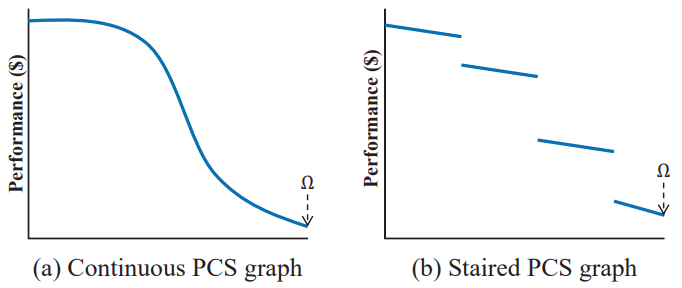
\includegraphics[width=0.8\linewidth]{Chapter-Introduction/Figures/stairs.png}
    \caption{Performance curves. (From ~\cite{oh2017finding})}
    \label{fig:chap1_stairs}
\end{figure}

To elaborate, if we sort the configurations from worst-performance to best and
plot configurations along the X-axis and performance along the
Y-axis. We expected a continuous graph
such as Figure~\ref{fig:chap1_stairs}(a), where high-valued (\$) is bad (worst performance is at the far left) and low-valued (\$) is good (best performance is at the
far right). Interestingly, Marker et al.~\cite{marker2014understanding} discovered that performance curves often occurs (in real world) as stairs, as in Figure 3b. Stairs arise from discrete feature decisions;
some features are highly-influential in performance while others
have little or no impact. Consequently, a few critical features
influences the performance while less important feature decisions alter the performance of nearby configurations only slightly (giving a stair its width and slope).

\noindent\textbf{Intuition}: From the literature, it is evident that most of the configuration options in a (given) software system does not affect the performance of the configurations. Hence, the central insight of this work is that random sampling with no regards to this specific feature of this problem is ineffective and hence adds additional cost. 

\noindent\textbf{Proposal}: This problem can be reformulated as a clustering problem, where we try to find an unsupervised method to cluster the configuration space into meaningful clusters. Once we have these clusters, we can use random samples (of configurations) from each of these clusters. This way, we can reduce redundant measurements.  

\section{Ranking}
Prior work in this area (including~\cite{nair2017faster}), tried to build accurate performance predictors, which can be used to predict the performance of a certain configuration. This work reflects on the prior work and asks: ``\textit{Our goal is to find a good configuration~\footnote{Good is defined as the distance from the optimal configuration} but, why does the prior work transform this problem into building an accurate model?}'' Another reason for this question is the very nature of the model building process previously described in Figure~\ref{fig:chap1_sampling_process}. We ask the question ``How does a user define \textit{Good}''? There is no way for the user to know whether a model can be build with MMRE less that 10\%. 

With respect to aforementioned questions, we drastically modify our approach to this problem. We hypothesize that to find the best performing configuration, we do not want a model which can return a predicted performance score which is as close to the actual performance score. Instead, we build a model which preserves the relative ordering of the configurations. 

\noindent\textbf{Intuition}: The central insight of this work is that exact performance
values (e.g., the response time of a software system) are not
required to rank configurations and to identify the optimal one. To elaborate more, let us assume that we have two humans (Adam---134cm, Billy---173cm) (analogous to configurations) and our objective is to identify the tallest person (Billy). To identify the tallest person, do we need a model which accurately predicts their height in a nano-meter scale? We can easily identify Billy even if the bad model predicted Adams height as 700cm and 890cm. 

\noindent\textbf{Proposal}: 
We show that, if we (slightly) relax the question
we ask, we can build useful predictors using very small sample sets.
Specifically, instead of asking ``How long will this configuration
run?'', we ask instead ``Will this configuration run faster than that
configuration?'' or ``Which is the fastest configuration?''.


\section{Sequential-Model Based Sampling}
Prior work in this area primarily used two strategies.
Firstly, researchers used machine learning to model the configuration
space. The model is built sequentially, where new
configurations are sampled randomly, and the quality or
accuracy of the model is measured using a holdout set. The
size of the holdout set in some cases could be up to 20\% of
the configuration space~\cite{nair2017using} and needs to be evaluated (i.e.,
measured) before even the model is fully built. This strategy
makes these methods not suitable in a practical setting since
the generated holdout set can be (very) expensive. Secondly,
the sequential model-based techniques used in prior work
relied on Gaussian Process Models (GPM) to reflect on the
configurations explored (or evaluated) so far~\cite{zuluaga2016varepsilon}. However,
GPMs do not scale well for software systems with more than
a dozen configuration options~\cite{wang2016bayesian}.



\noindent\textbf{Intuition}: 
To reduce the cost of sampling and eliminate the need for holdout set, we use sequential Model-based Optimization (SMBO). SMBO uses the Bayesian methodology to the iterative optimizer by incorporating a prior model (built using configuration which are already measured) on the space of possible target functions, $f$. By updating this model every time time a configuration is evaluated, a SMBO routine keeps a posterior model of the target function $f$. This posterior model is the surrogate $f^*$ for the function f (ground truth). Figure~\ref{fig:chap1_smbo} encapsulates the process.

\begin{figure}[!htbp]
    \centering
    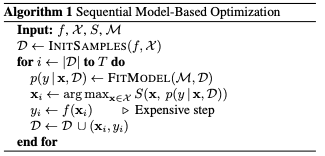
\includegraphics[width=0.6\linewidth]{Chapter-Introduction/Figures/bayesian_opt.png}
    \caption[Algorithm for SMBO methods]{Sequential Model-based Optimization. (From ~\url{http://tiny.cc/3hy80y})}
    \label{fig:chap1_smbo}
\end{figure}

\noindent\textbf{Proposal}:
We use the intuition present above to develop a method called FLASH.
The key idea of FLASH is to build a performance model
that is just accurate enough for differentiating better configurations
from the rest of the configuration space. Tolerating
the inaccuracy of the model is useful to reduce the cost
(measured in terms of the number of configurations evaluated)
and the time required to find the better configuration.
To increase the scalability of methods using GPM (Gaussian Process Models)---used widely in the machine learning domain, FLASH
replaces the GPMs with a fast and scalable decision tree learner.





\section{How to Read the Dissertation}
This dissertation is organized as self-contained chapters that together support
the thesis.

\textbf{Chapter~\ref{chapter:one}} explains, identifies and provides context for the research problem, articulates the objective, significance, and scope of the work.

\textbf{Chapter~\ref{chapter:background}} presents the background and related work in this area. The area of performance optimization has been explored not just in the domain of software engineering and has gained a lot of interest in the systems community as well. In general, there has been a considerable interest in the black-box optimization literature. In this chapter, an attempt has been made to describe the research work using the terminology used in the rest of the thesis.

\textbf{Chapter~\ref{chapter:WHAT}} describes the design and implementation
of \emph{WHAT}.
{\what}'s innovation is  
the use of the spectrum (eigenvalues) of the distance matrix
between the configurations of a configurable software system, to perform dimensionality reduction. Within that
reduced configuration space, many closely associated configurations can be studied
by executing only a few sample configurations. For the subject systems studied
here, a few dozen samples yield accurate and stable predictors---less than 10\,\% prediction error, with a standard deviation of less than 2\,\%.  
When compared to the state of the art, our approach (a)~requires 
2 to 10 times fewer samples to achieve similar prediction accuracies,
and (b)~its predictions are  more stable (i.e., have lower standard
deviation). 
Furthermore, we demonstrate that predictive models generated by
\what can be used by optimizers to discover system configurations that closely approach the optimal performance.


\textbf{Chapter~\ref{chapter:rank}} proposes using ranking models instead of regression models to save cost while finding good configurations. The central  insight of this chapter is that   
exact performance values (e.g., the response time of a software system) are not required to rank  configurations and to identify the optimal one. 
As shown by our experiments, performance models that are cheap to learn but inaccurate (with respect to the difference between actual and predicted performance) can still be used rank configurations and hence find the optimal configuration. This novel \emph{rank-based approach} allows us to significantly reduce the cost (in terms of number of measurements of sample configuration) as well as the time required to build performance models. We evaluate our approach with 21 scenarios based on 9 software systems and demonstrate that our approach is beneficial in 16 scenarios; for the remaining 5 scenarios, an accurate model can be built by using very few samples anyway, without the need for a rank-based approach.

In \textbf{Chapter~\ref{chapter:flash}}, we design and implement FLASH. The central insight of this paper is to use the prior knowledge (gained from prior runs) to choose the next promising configuration. This strategy reduces the effort (measured in terms of the number of measurements) required to find the (near) optimal configuration.  \flash can be used to solve single-objective (e.g., run-time) and can also be adapted to multi-objective (e.g., energy and runtime) performance optimization problems. 
We evaluate \flash  using 30 scenarios based on 7 software systems to demonstrate that \flash saves effort in 100\% and 80\% of cases in single-objective and multi-objective problems respectively by up to several orders of magnitude. 
% We also demonstrate how \flash is more scalable than other state of the art sequential model-based methods. 
% \textcolor{red}{TODO}
% Many design processes can be described as the exploration of options. Hence, 
% \flash can be applied to many areas.
% To demonstrate this,  we evaluate \flash, beside performance configuration optimization,  on standard search-based software engineering case studies   (release planning, process modeling, and sprint planning for agile development). 
% The superior performance
% of  \flash in these software systems, plus its better scalability and faster runtimes, makes us recommend this method XXX

In \textbf{Chapter~\ref{chapter:conclusion}}, we revisit the key contributions of this thesis and provide directions for future work.
\chapter{Background and Related Work}
\label{chapter:background}

This chapter describes the necessary background that is related to
the research problems addressed in this dissertation.
We first describe data-intensive computing and its storage architecture.
Next we discuss performance prediction for distributed systems.
Last, we discuss related work that uses the data-driven approach
to optimize system performance.



\chapter{End-to-End Performance Prediction for Cloud Storage}
\label{chapter:inside-out}

This chapter presents an approach to estimating end-to-end performance
of distributed storage systems.
We explain why low-level performance metrics are a desirable proxy
for estimating end-to-end performance.
We then present our automatic model building tool for generating
robust and accurate performance models.

\section{Introduction}
\label{ch4:sec:introduction}

Many storage systems are moving away from dedicated appliance-based storage model to software-defined 
storage (SDS), which separates software that provisions and manages storage from the hardware that provides raw physical storage~\cite{sds_att, Thereska2013, Jalaparti2012}.
This trend is partly driven by the tremendous growth of data and the emergence of cloud applications that operate in a multi-tenant environment with diverse workload characteristics.
As a result, the rigid appliance-based model, with tightly-coupled hardware and software features, is no longer cost-effective, lacks flexibility, and does not scale well.
SDS systems are increasingly abandoning centralized storage services in favor of distributed systems like Ceph~\cite{ceph}, HDFS~\cite{hadoop}, Swift~\cite{openstack}. 
Distributed storage systems are attractive because they scale well, allowing storage services to grow or shrink, based on storage demands. 
They are also better suited to handle diverse multi-tenant workloads. 

Providing reliable quality of service (QoS) to storage applications is critical in an SDS environment shared by multiple applications 
with diverse usage patterns. However, in a distributed storage environment, it is challenging to provide storage QoS in a consistent 
and reliable manner. Practical deployments of modern distributed storage systems like Ceph are composed of a large number of 
individual storage components that can interact in a complex manner. 
Diverse and time-varying storage workloads and performance interference in a multi-tenant environment further 
complicate the reliable assurance of storage QoS. Reliable and accurate monitoring of 
high-level storage performance metrics (e.g. throughput and IOPS) is critical 
for providing storage QoS guarantees.    
However, monitoring end-to-end storage performance is difficult in a distributed storage service. 
Instrumenting user applications to measure storage performance is not always practical. 
Performing benchmark tests in production systems also has practical limitations since they 
interfere with storage application workload.
Furthermore, running exhaustive benchmark experiments to cover diverse application workloads, 
deployment topologies, and large configuration parameter space is time-consuming and impractical in many cases. 
Building accurate analytical performance models, on the other hand, is also difficult for the reasons mentioned above.
 
This chapter proposes the idea of using low-level system metrics (e.g., CPU usage, RAM usage and network I/O)
as a proxy for measuring high-level performance (e.g., end-to-end IOPS and throughput) of 
distributed storage applications.
We design, implement and evaluate a practical tool, called \emph{Inside-Out}, that applies 
machine learning techniques to the low-level metrics collected from individual components 
of a distributed storage system to accurately estimate high-level storage performance metrics---like throughput and IOPS---of the entire 
distributed storage system.
We believe that a tool like Inside-Out can serve as an important component of the overall SDS architecture.

Inside-Out takes a black-box modeling approach, which does not require knowledge about distributed storage system protocol, workload characteristics, and deployment topology. 
Inside-Out relies upon machine learning techniques to automatically derive an accurate end-to-end performance model.
We explore several well-known machine learning algorithms including linear regression, 
decision tree learning, and ensemble methods \cite{Wang2004, Noorshams2013}, and conclude that  
there does not exist an one-size-fits-all algorithm that can work in all prediction cases.
Hyperparameter tuning \cite{Chapelle2002, Noorshams2013}, model selection \cite{Kohavi1995} and 
feature selection \cite{guyon2003introduction, Saeys12007} all turn out to be too complicated for optimizing prediction accuracy.
In contrast, Inside-Out uses a two-level learning method that automatically selects important features, boosts prediction accuracy, and achieves consistent prediction. 
This two-level learning method pipelines two supervised learning algorithms to eliminate irrelevant features while avoiding overfitting problems.\footnote{\label{ft:overfitting}
Overfitting describes the situation when a model captures the relationship of noisy data but not the underlying relationship \cite{domingos2012few}.
Overfitting becomes more prominent in the presence of high dimensional data}

Inside-Out offers several key benefits. 
%[MRA] Unlike traditional analytic performance modeling approach, Inside-Out is generic in nature, and therefore, it can be applied to different storage services.  
Unlike traditional analytic performance modeling approach, Inside-Out is more generic, 
and therefore can be more easily applied to different storage services.  
Different from previous work, Inside-Out 
does not require information about system configuration and application workload~\cite{Ruemmler1994, Shriver1998, Wang2004, Kelly2004, Yin2006, Noorshams2013, Ardagna2014}. 
Due to the self-learning property, \emph{Inside-Out} improves performance prediction accuracy with more data.
It can also adapt to changes in the system
by continuously learning the system behavior. 

We evaluate Inside-Out using Ceph~\cite{ceph} %as an example distributed storage system 
running on an OpenStack-based SDS platform.
The low-level performance metrics are collected from participant virtual machines 
running various components of a Ceph storage service.\footnote{\label{ft:vm}
Our approach is not limited to VM-based environments.
It can be applied to container-based and bare-metal storage servers as well.
}
Our in-depth evaluation shows that Inside-Out generates end-to-end performance models with 91.1\% prediction accuracy on average.
More importantly, as discussed above, Inside-Out is generic in nature as it captures the behavior of the storage system 
by analyzing low-level system metrics (that are protocol and application agnostic). Furthermore, we demonstrate that Inside-Out 
%[MRA] can provide reliable performance monitoring even in the presence of evolving workload characteristics, changing storage 
can provide reliable hints for performance monitoring tasks even in the presence of evolving workload characteristics, changing storage 
configuration and interfering tenants. We also show that Inside-Out is reliable in estimating end-to-end performance 
even when the storage system expands or shrinks.
We show that Inside-Out provides reliable performance 
prediction when the storage system is up to four times larger than the one used for building machine learning models during 
the training phase. 
Lastly, Inside-Out is able to learn new storage behavior over time.
\section{Mapping from Low to High}
\label{sec:challenges}

%[commented by MRA] We discuss how to use low-level performance metrics collected from distributed components to build an accurate end-to-end performance model for a distributed storage system in the SDS environment.
This section discusses the guiding principles and challenges in using low-level performance metrics
to build accurate end-to-end performance models for a distributed storage system.
%collected from individual components of a 
%distributed storage system for building an accurate end-to-end performance model.

%\subsection{Searching for Representative Features}
\subsection{Important Considerations}

This section describes how we use low-level performance metrics
to predict high-level system performance.
We discuss how we pick the metrics and how to transform metrics
to meaningful features.

\label{sec:feaatures_for_distributed_system}

%[commented by MRA] We have to keep in mind that we are developing a tool that can apply to diverse storage services to be deployed in SDS.
%Manually building models for each storage service requires energy and cost that are several times more than an automatic and general approach.
%Note that we are developing a tool that can be applied to a diverse set of storage systems and services.
%Manually building a model for each storage service requires more effort and cost compared to an automated 
%and general, i.e., application-agnostic, approach.

%\subsubsection{Requiring general performance metrics}
\subsubsection*{General low-level metrics}
%
%Low-level performance metrics are general and application independent.
Since our goal is to provide a tool for estimating the end-to-end performance of a diverse set of 
storage systems, the inputs to our model need to be generic in nature, \ie they need to 
be independent of storage systems or the distributed protocols used by such applications. An SDS provider 
should be able to obtain the input metrics without instrumenting storage application or requiring domain 
knowledge about the storage application. Low-level system metrics (e.g. CPU utilization, memory usage, network IO, etc.) 
satisfy these requirements. DeepDive uses low-level metrics to identify performance anomaly for a running VM~\cite{Novakovic2013}. 
To the best of our knowledge, this work presents the first study that maps low-level system metrics to 
high-level end-to-end performance of a distributed storage service.

%Low-level performance metrics are application independent.
%An SDS provider can obtain this information without instrumenting applications.
%For example, DeepDive~\mra{citation?} use low-level metrics to identify performance anomaly for a running VM \cite{Novakovic2013}.
%To the best of our knowledge, this paper presents the first study that maps low-level performance metrics to high-level end-to-end performance of a distributed storage service.

\begin{figure}
\centering
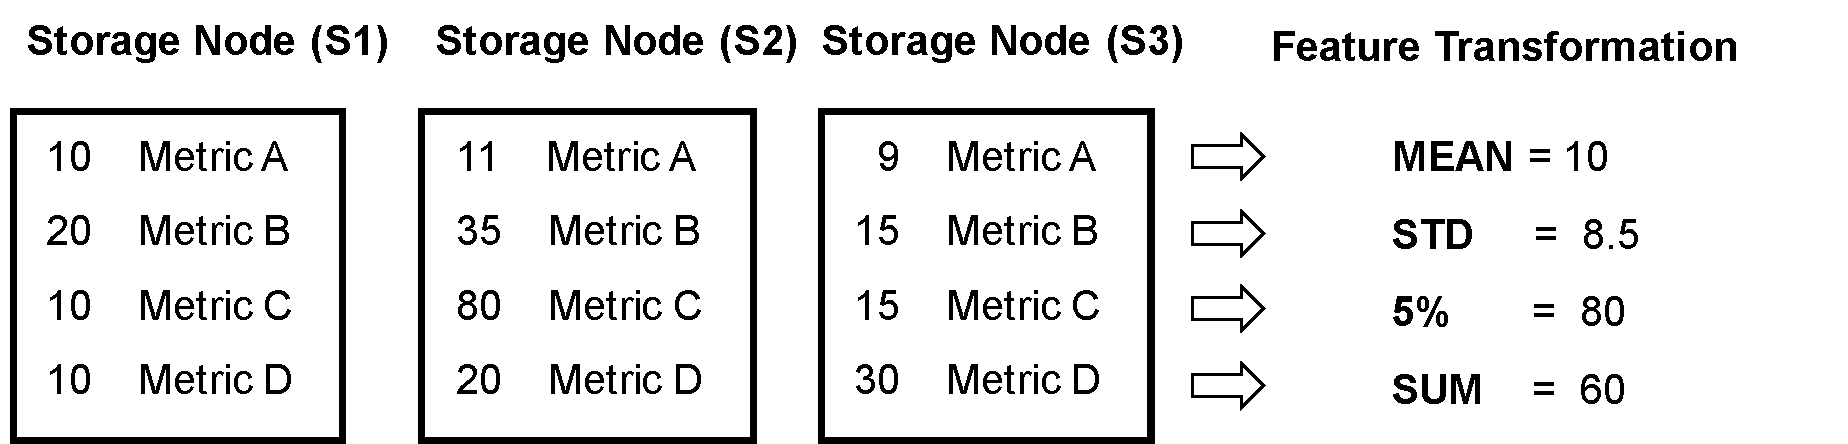
\includegraphics[width=0.9\textwidth, keepaspectratio]{figures/features.pdf}
\caption{Four statistical features used in Inside-Out to capture load and internal status of a distributed storage system.  The numbers and metrics represent low-level performance data collected from storage nodes.}
\label{fig:feature_types}
\end{figure}


%\subsubsection{Handling the distributed system scenario}
\subsubsection*{Capture important features of a distributed storage system}
%
%One important characteristic of a distributed storage system is that it can expand or shrink on demand 
A distributed storage system can dynamically expand or shrink
according to demand.
The performance model has to capture the current 
scale of the deployment, the bottlenecks, and the average and variance in performance
of individual components of the distributed system. For each low-level system metric collected from 
various components of the distributed system, we use four statistical variables to characterize the behavior of a distributed system (see \myfigure{\ref{fig:feature_types}}). 
The statistical variable \textit{mean} and \textit{std} describe whether the impact of the workload is evenly distributed among 
storage components. The \textit{sum} variable represents the scale of the deployment, while the variable \textit{5\%} (top 5 percentile) captures the hot spot situations. 
The feature transformation from raw system metrics to these four statistical values also allows Inside-Out to apply 
the uniform input format for developing performance models for distributed systems at different scales.

\subsection{Feature Selection}
\label{sec:non-deterministic}

In this work, we collect low-level performance metrics
from two components of Ceph
namely monitor (MON) and Object Storage Daemons (OSD).
We use \emph{dstat}, a monitoring tool to collect resource statistics,
to collect 32 low-level performance metrics in total.
These measurements are then transformed using the process described in \myfigure{\ref{fig:feature_types}} (refer to Section~\ref{sec:data_preprocessing} for more details).


Selecting the ``right'' features from high dimensional data
is a challenging task because
as computation complexity increases, prediction accuracy may decreases
~\cite{guyon2003introduction, Saeys12007}.
Furthermore, for our case, the right feature set is not always the identical.
Table \ref{tab:challenge_feature_selection} shows the \emph{model accuracy} of different learning methods when modeling 
read throughput. 
%\chin{
%verified with $10$-fold cross validation.
%}
We see that all learning methods achieve high model accuracy
even though they choose different features. 
The model accuracy was obtained using $k$-fold cross validation (\textit{k}=10),
a common technique for assessing model accuracy. 
The training data is partitioned into $k$ disjoint sets. 
A single data partition is used for validation purpose and the remaining $k-1$ partitions are used for training data.
Although all models yield good model accuracy, they perform poorly and inconsistently when the storage environment changes. 
In \myfigure{\ref{fig:challenge_generalization}},
we show the prediction accuracy under
%we show prediction accuracy when we make
three types of changes in the storage environment---increase in the size of the distributed 
storage system, read workload and individual storage IO request size.
These algorithms (discussed later in Section~\ref{sec:algorithm_selection}) do not yield consistent prediction accuracy any more. 
For example, Lasso can still predict well when workload has changed but Decision Tree cannot.
On the contrary, Decision Tree performs better than Lasso when the size of the storage system increases.
We suspect this is caused by the large feature space, which leads to the overfitting problem \cite{domingos2012few, hastie2005}.
Next, we manually remove most features and select only a few with a trial-and-error strategy.
As shown in \myfigure{\ref{fig:challenge_generalization}}, we see significant improvement in some cases, but not all. 
Since an SDS environment can change over time, it is important for our model to provide consistent prediction accuracy under system changes
such as software reconfiguration and cluster expansion.


\begin{table*}[t!]
\caption{Important features selected by different algorithms are not deterministic}
\centering
\label{tab:challenge_feature_selection}
%\begin{tabular}{|lll|lll|lll|lll|lll|}
%\resizebox{!}{.8\linewidth}{
\resizebox*{\textwidth}{!}{
\begin{tabular}{|lll|lll|lll|lll|lll|}
%\begin{tabularx}{1.0\linewidth}{|lXl|lXl|lXl|lXl|lXl|}

\hline
\multicolumn{3}{|c|}{\textbf{Lasso}}   & \multicolumn{3}{c|}{\textbf{Ridge}}   & \multicolumn{3}{c|}{\textbf{Elastic Net}} & \multicolumn{3}{c|}{\textbf{Decision Tree}} & \multicolumn{3}{c|}{\textbf{Random Forest}} \\
\hline
osd  & network.send  & sum  & \textbf{osd}  & \textbf{network.recv}  & \textbf{mean} & osd   & network.send   & sum    & osd    & disk.read       & sum    & osd    & disk.read       & sum    \\
osd  & disk.writ     & sum  & \textbf{osd}  & \textbf{disk.read}     & \textbf{5\%}  & osd   & disk.writ      & sum    & osd    & network.send    & sum    & osd    & network.send    & sum    \\
\textbf{osd}  & \textbf{cpu.sys}       & \textbf{sum}  & \textbf{osd}  & \textbf{load.15m}      & \textbf{std}  & osd   & disk.read      & sum    & osd    & network.recv    & sum    & osd    & disk.writ       & sum    \\
osd  & io.read       & sum  & osd  & network.send  & sum  & osd   & cpu.sys        & sum    & osd    & disk.writ       & sum    & \textbf{osd}    & \textbf{network.recv}    & \textbf{sum}    \\
osd  & vm.minpf      & mean & osd  & tcp.tim       & std  & osd   & tcp.lis        & sum    & \textbf{mon}    & \textbf{memory.buff}     & \textbf{mean}   & osd    & memory.cach     & sum    \\
\textbf{mon}  & \textbf{memory.used}   & \textbf{5\%}  & osd  & network.recv  & std  & osd   & io.read        & std    & osd    & cpu.sys         & sum    & osd    & memory.buff     & mean   \\
\textbf{mon}  & \textbf{memory.cach}   & \textbf{5\%}  & osd  & load.5m       & std  & osd   & io.read        & sum    & osd    & vm.alloc        & sum    & osd    & memory.buff     & 5\%    \\
osd  & tcp.lis       & sum  & osd  & cpu.idl       & sum  & osd   & vm.minpf       & mean   & osd    & vm.minpf        & 5\%    & mon    & io.writ         & sum    \\
osd  & io.read       & std  & osd  & cpu.wai       & sum  & osd   & io.writ        & mean   & \textbf{mon}    & \textbf{cpu.idl}         & \textbf{std}    & osd    & memory.buff     & sum    \\
osd  & io.writ       & mean & osd  & cpu.sys       & sum  & \textbf{mon}   & \textbf{memory.used}    & \textbf{sum}    & mon    & memory.cach     & sum    & mon    & vm.free         & sum    \\
\hline
\multicolumn{3}{|c|}{96.20\%} & \multicolumn{3}{c|}{96.60\%} & \multicolumn{3}{c|}{96.18\%}     & \multicolumn{3}{c|}{96.78\%}       & \multicolumn{3}{c|}{96.94\%} \\
\hline
\end{tabular}
%\end{tabularx}
}
\end{table*}



\begin{figure*}
    \centering
    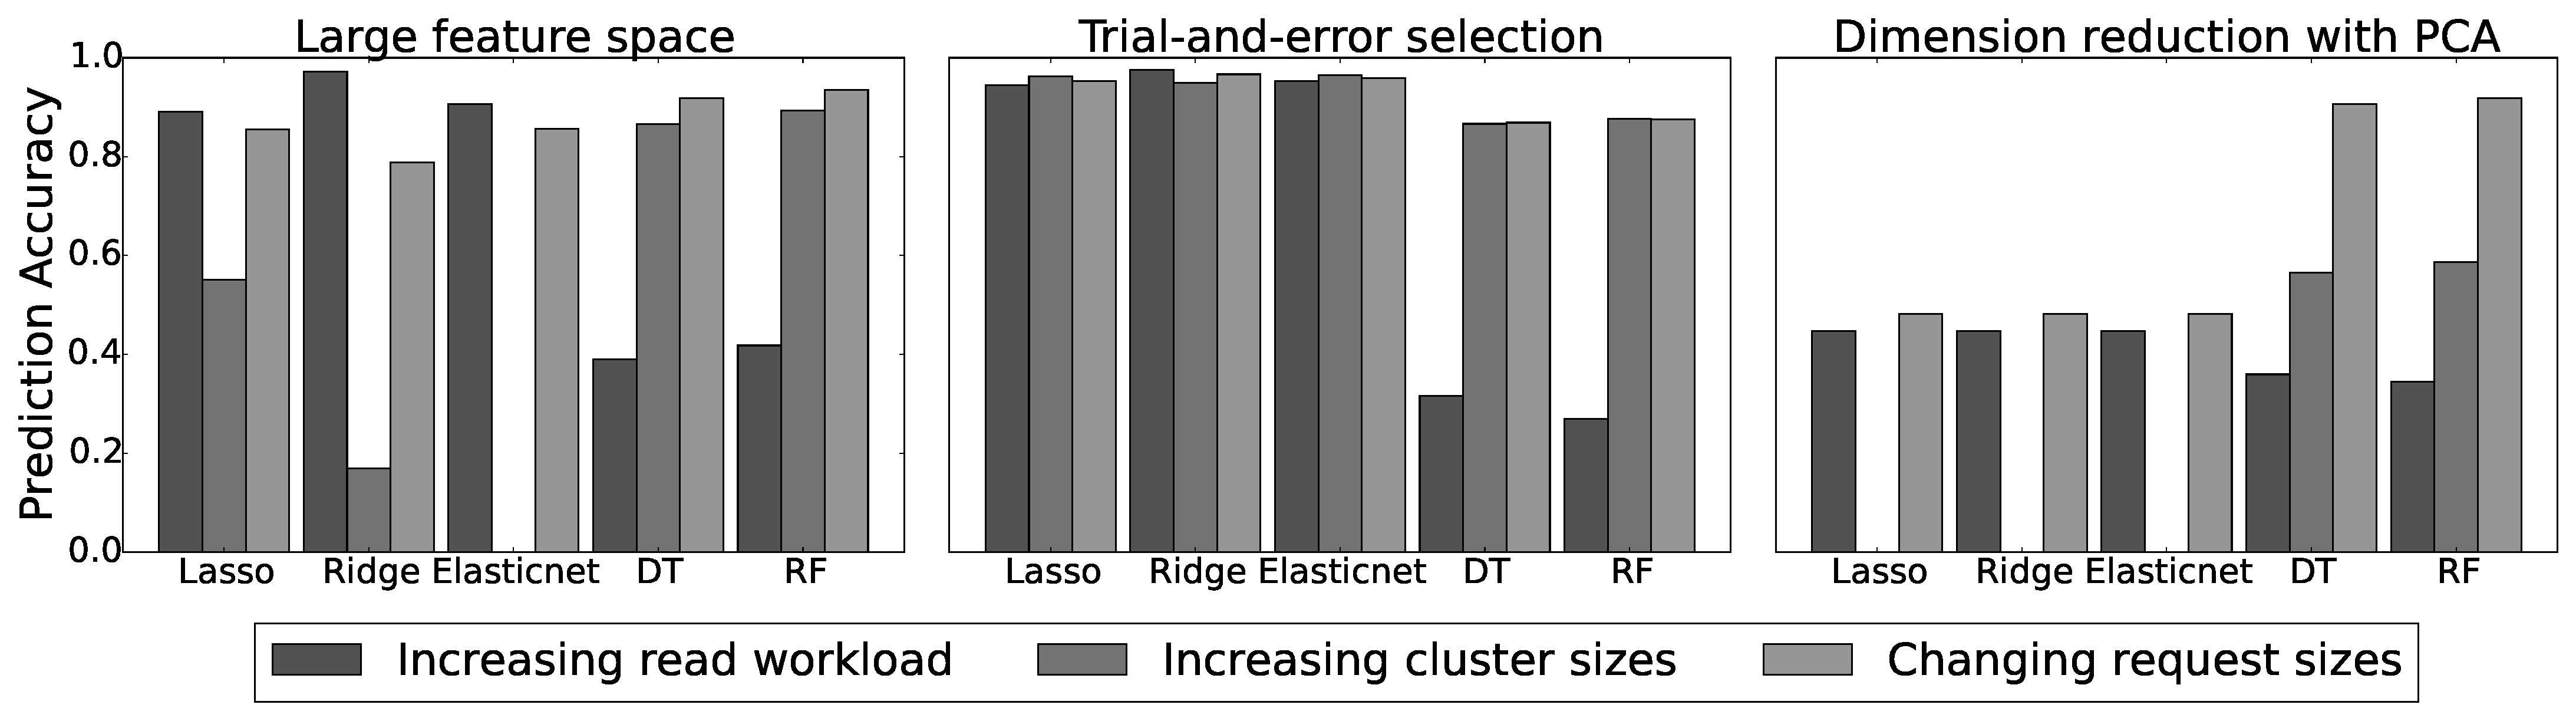
\includegraphics[width=1\textwidth]{figures/challenge_generalization_combined_horizental.eps}
    \caption{Prediction accuracy is inconsistent due to the large feature space.
    Learning methods fail to select the right features in some cases.
    Dimension reduction (PCA with 10 components) does not help in this case.
    In the trial-and-error case, we select a subset of metrics, e.g. \emph{mean(disk.read)}, \emph{sum(network.recv)} and \emph{std(cpu.usr)}.}
    \label{fig:challenge_generalization}
\end{figure*}

Although Hyperparameter tuning, model selection, and 
feature selection have been proposed as potential solutions, it is challenging 
to use them in practice, not to mention the complexity of automating this task. 
PCA (Principle Component Analysis) is another potential solution \cite{Shlens2003}.
PCA transforms original data into a lower dimension while keeping high fidelity.
However, PCA has several limitations. 
First, PCA is not scale invariant.
Not all performance metrics are comparable and therefore, there is no standard way to scale these metrics.
Second, PCA assumes Gaussian distribution in data points; however, many storage workloads have Pareto distribution \cite{Kim2010}.
Third, determining a good number of components is also a challenging task.
In our case, PCA does not address the problems.
In fact, \myfigure{\ref{fig:challenge_generalization}} shows that it can further degrade prediction accuracy.

\subsection{A Two-Level Approach}

Instead of performing feature selection or dimension reduction, we propose a generic two-step approach that can improve the consistency of prediction accuracy. 
In the first step, we use some heuristic methods to filter out irrelevant features.
Then, in the second step, we apply machine learning algorithms to build performance models with the reduced feature set.
The intuition behind this idea is that it is difficult to determine the most important performance features but it is relatively easy to eliminate unimportant features.
For example, the features which are not in the top 100 list after step one can be labeled as unimportant features.
\section{The Inside-Out Design}
\label{sec:methodology}
%\rp{Chin: In the previous section, you say ``As we will explain in Section V-A, we use 32 low-level performance 
%metrics collected with dstat''. This section does not say anything about 32 metrics. Please mention them here. 
%I think we need to write this section in a much better way. You should clearly explain the steps: something like: We collect 32 
%low level system metrics from each VM (either give the list or mention just the few) every x seconds. Then say we take mean, std, sum and 5\% of each 
%of these 32 metrics for every moving window of xxx seconds. Then explain why we use moving window. then say that for training and validation purposes, 
%we measure the end-to-end performance metrics (IOPS, throughput, and latency) using cosbench every x seconds. Then we take average, xxx, xxx etc. 
%of these metrics ...I think you get the point now, right? We have to clearly explain what we exactly did. }
In this section, we present the design of Inside-Out.
We also discuss the trade-offs among a set of representative machine learning algorithms
and propose a two-step learning technique for mitigating overfitting problems.



\subsection{Collecting and Pre-Processing Low-Level Metrics}
\label{sec:data_preprocessing}

Inside-Out collects general, low-level system metrics from individual machines running the distributed storage service.
However, the raw collected data suffers from various problems due to inefficiency of data collectors, system clock skews,
incomparable data formats, workload outliers, bursty system anomalies, \etc
The noisy data can lead to unstable and 
inaccurate performance models. 
Inside-Out performs a series of data pre-processing functions to address these issues.

%\rp{The goal of this step is to remove unwanted characteristics of the collected data, such as
%workload outliers, system clock deviation, incomparable data format, etc.
%}


%Data preprocessing is a preparation step before training a model.


\subsubsection{Monitoring storage components}
We collect low-level system metrics of the underlying operating system to capture resource utilization 
(\eg cpu, memory, disk and network usage).  
The low-level performance metrics are sampled with one-second granularity.
Such data can be collected from \textit{libvirt}, Ganglia, instrumented hypervisors \cite{Koh2007} and \textit{Ceilometer} in OpenStack.
We use  \emph{dstat} monitoring tool (with option: -tcly -mg --vm -dr -n --tcp --float) to collect these data.


%This step helps us eliminate unwanted characteristics of the collected data, such as
%high variation due to workloads, uncertainty originated by physical hardware, 
%system clock deviation, incomparable data format, etc.
%For the collected performance data, fluctuating metrics, time synchronization and feature transformation for a distributed system are the major challenges.

%\subsubsection{Smoothing monitored data}
\subsubsection{Data smoothing}
%
Building a performance model with data collected at one-second granularity is challenging because 
system data can exhibit high variance at small time scales, \eg due to dynamic/bursty workloads and interference among co-located tenants.
Furthermore, the storage IO operation needs to pass through a series of software layers 
between the storage client and the back-end raw physical storage device. 
The long storage IO path can introduce high variability in resource utilization at smaller time scales. 
For example, HDFS and Ceph both replicate data blocks across storage nodes distributed in physically disjoint 
servers, racks or even datacenters.
To address the uncertainties due to complex IO path spanning several software layers, 
we compute the moving average of the collected performance data.
We have empirically found that one-minute window for processing the moving average is sufficient to 
eliminate outliers from the raw data.
%we use moving averages to construct a stable prediction model.
%We choose one-minute windows for moving average since we have empirically found 60-second moving averages to smooth out raw data sufficiently, without 
%compromising data quality, in order to yield stable and accurate performance models.
%A fine granularity, at lease 15 seconds, is also desirable from our experience.

%RP: Chin, I commented the following line becuause it looks too vague. If you want to clarify this, 
%we can restate in a better way. 
%and the uncertainty come from the interaction between software and hardware components.
%We use moving average to smooth the collected performance data for stable prediction model.
%\rp{Chin: Please explain ``moving average of xxx'', ``why 15 seconds is a desirable window''. These aspects need to be mentioned 
%in a clear manner, not in a handwavy way.}
%We use moving average to construct a stable prediction model.
%Based on our data collected from our internal testbed, 
%it is desirable to use a window greater than 15 seconds. 
%From our experience, a window greater than 15 seconds shows stable results.
%One reason is that a storage request can last longer than 10 seconds for accessing large objects (or files).

\subsubsection{Timestamp alignment}
Proper time synchronization among participating servers is essential to correlate data collected from those servers. 
We use NTP for time synchronization.
The average timestamp of all nodes is taken as the basis for time alignment.

\subsubsection{Feature transformation for a distributed storage system}
%
As mentioned earlier, elasticity is an important feature of SDS, since it needs to adjust its size based on storage demand. 
%The built prediction model needs to be able to predict end-to-end performance at different system scales.
Thus our model must accurately predict end-to-end performance at arbitrary deployment scales.
However, the data collected from different scales may have different dimensions. 
For instance, Ceph with 10 Object Storage Servers (OSDs) generates 10 copies of low-level performance metrics, 
while Ceph with 5 OSDs generates fewer data points. This makes it hard to train and build a unified model.
As mentioned in Section~\ref{sec:feaatures_for_distributed_system}, we use \emph{mean, sum, std, and 5\%} statistical 
variables to capture 
different types of workload distribution such as
\emph{hotspot}, \emph{load imbalance}, and \emph{aggregate performance}.

%To achieve the goal, we need to make sure the dimension of data, collecting from different system configurations are comparable.
%As suggested in Section~\ref{sec:feaatures_for_distributed_system}, our feature transformation describes a distributed system as in one of the four conditions: load-balancing, non-load-balancing, hotspot and the aggregate workload.
%As suggested in Section~\ref{sec:feaatures_for_distributed_system}, our feature transformation process 
%takes four conditions into account: load-balancing, non-load-balancing, hotspot and the aggregate workload.

In summary, Inside-Out collects 32 raw low-level system metrics with one-second granularity.
Inside-Out applies proper time alignment and moving average with one-minute windows for stabilizing performance data.
Then it calculates \emph{mean}, \emph{std}, \emph{sum} and \emph{5\%} of individual metrics collected from multiple machines.
This ensures that our performance model can accept input data for systems with varying scales of deployment, 
while preserving important characteristics of a distributed storage system.
For training and validation purposes, 
we measure end-to-end performance metrics (IOPS, throughput, and latency) every 5 seconds using COSbench \cite{cosbench}, and take average over the one-minute window.
Next, we describe how we build end-to-end performance models in order to capture the relationship between low-level system metrics and end-to-end throughput and IOPS.

%Lastly, we transform low-level performance metrics to create comparable dataset while preserving characteristics 
%of a distributed storage system, using the feature transformation specified in Figure~\ref{fig:feature_types}.

%In summary, we use a 60-seconds window to smooth performance data, and proper time alignment has applied to the monitored performance data.
%\mra{Chin, what did you use to transform the data? average? It would be good if we can briefly state how we transform the data.
%if you already described this somewhere later in the paper, we could forward reference the section.}


\subsection{Exploring Learning Methods}
\label{sec:algorithm_selection}

%We collect time series data composed of low-level system metrics collected from all machines running the distributed storage system. 
%At each sampling time (every $t$ seconds), a low-level performance snapshot of a running distributed storage system is \rp{obtained from} the dataset.
%Given a performance snapshot at time $t$ of a running distributed storage, we aim to build a model that predicts the storage's end-to-end performance, e.g. throughput and IOPS.
%The performance snapshot is the low-level performance metrics collected from distributed storage nodes.

Our goal is to build a model that accurately predicts end-to-end throughput and IOPS by analyzing only the low-level metrics of a distributed storage system.
We explore several algorithms, including statistical regression \cite{Fron2004, hastie2005}, 
decision tree learning and random forests learning \cite{hastie2005,Wang2004}.
For statistical regression, we mainly focus on linear regression techniques, 
which can be extended to support non-linear regression by expanding features that simulate, 
for example, quadratic terms \cite{Kundu2010}.
We did not find this necessary in our application and exclude the discussion.

%\subsubsection{Lasso}
%\textit{Lasso\footnote{Least Absolute Shrinkage and Selection Operator}} 
% remove the full name above
\textit{Lasso} 
is a least square linear regression technique with L1-norm regularization.
The L1 penalty function leads to a sparse solution, which has an effect of restricting 
the number of selected variables.
This property is useful for figuring out important features, especially 
when the number of variables or features is large.
%
%\subsubsection{Ridge}
\textit{Ridge} is similar to Lasso but instead uses L2-norm regularization, 
which has the effect of group selection of variables.
This property does not restrict the number of variables selected by the prediction model 
and therefore, the prediction accuracy might degrade and become inconsistent 
%when the feature space is large.
when the number of input features to the training model is large. 
%when we use a small number of features out of much larger feature space.
%\mra{Chin, I modified the previous sentence. Check if it is ok with you.}
%
%\subsubsection{Elastic Net}
\textit{Elastic Net} combines both advantages---it does group selection while enforcing sparsity.
Based on our data set, Lasso and Elastic Net have similar prediction performance, and Ridge shows larger variance.
%
The \textit{Decision Tree} (DT) learning uses a top-down approach and recursively partitions data to fit target values.
The tree-based model is easy to interpret and scales well to large datasets.
\textit{Random Forests} (RF) is an ensemble method that uses multiple decision trees~\cite{hastie2005}.
%In practice, it is accurate, efficient, and more robust compared to a single decision tree.
RF improves a single decision tree in many ways, e.g., accuracy, efficiency, and robustness.
%Due to space limit, please refer to \cite{hastie2005} for detailed description.

To summarize, linear regression models assume a linear relationship and might oversimplify the storage behavior. 
Nonetheless, it has the potential to exhibit better generalization for extrapolating performance prediction 
for the unknown behavior case (the pattern not included in the training dataset).
On the other hand, the tree-based learning can achieve good model accuracy (perfectly fits the training data), 
but it can easily lead to overfitting problems.
Its prediction accuracy decreases, for example,
under different storage workloads,
as shown in \myfigure{\ref{fig:challenge_generalization}}.


\subsection{Two-level Training}
\label{sec:auto_feature_selection}

%As discussed in Section~\ref{sec:non-deterministic}, 
The fundamental challenge 
in building an effective prediction model from a large set of features is the overfitting problem.
One way to address this problem is to perform manual feature selection.
However, this approach is problematic because the right set of features depend on application types, 
deployment topology, resource constraint, etc.

Instead, we propose a two-level training process that filters out irrelevant features in the first step 
and then builds models by using the reduced set of features in the second step.
To this end, Inside-Out pipelines Ridge and Lasso together, where Ridge filters features in 
coarse-granularity and then Lasso builds the prediction model.
We choose Ridge as the filtering algorithm because it is not a sparse solution and considers all features. 
We then apply exhaustive grid search to find the optimized score for important features.
We use $\alpha \times$ \textit{median(coefficients)} derived from Ridge as the threshold.

For comparison, we consider Decision Tree with Lasso (Auto-DTL) and RandomForest with Lasso (Auto-RFL).
Our evaluation shows Inside-Out outperforms consistently across all prediction cases, 
and boosts prediction accuracy in several scenarios, where the linear regression models 
fail to generalize the behavior of a distributed storage system.
We also experimented by using Lasso and Elastic Net as the filter algorithm but did not find comparable performance with Inside-Out.
%Beside, we also evaluated Lasso and used Elastic Net as a filter algorithm and 
%found they are not comparable with Auto-RL.
%\mra{this sentence is a little confusing..}
%We will leave them as future work to further study the major difference.

Inside-Out uses the following pseudo code to generate an end-to-end performance model.
In practice, we set $k$ to $10$ for stable prediction results.
The data processing part is explained in previous sections.
Features are automatically selected using the Ridge algorithm
with multiple thresholds.
We vary $\alpha$ from $0.1, 0.2, ..., 1.0$.
The grid search approach is used to select the best model.


 \begin{algorithm}
 \caption{Inside-Out Model Building}
 \begin{algorithmic}[1]
 \renewcommand{\algorithmicrequire}{\textbf{Input:}}
 \renewcommand{\algorithmicensure}{\textbf{Output:}}
 \REQUIRE low-level performance metrics from distributed nodes
 \ENSURE  an end-to-end performance model
 \\ \textit{Initialisation}
  \STATE $thresholds = \left \{ \alpha_{1}, ... , \alpha_{N} \right \} $\
  \STATE $m1 =$ filtering algorithm $\rightarrow Ridge$
  \STATE $m2 =$ model algorithm $\rightarrow Lasso$
  \STATE $k =$ k-fold cross validation
  \STATE $score = 0$
 \\ \textit{Data preprocessing} (refer to Section~\ref{sec:data_preprocessing})
  \STATE alignment of input data
  \STATE calculate moving average across metrics
  \STATE feature transformation for the distributed scenario
 \\ \textit{Grid Search}
  \FORALL{$t \in thresholds$}
  \STATE $features =$ execute $m1$ with threshold $t$
  \STATE $score, m = $max(crossvalidation($k$, $m2$, $features$))
  \ENDFOR
 \RETURN $m$ with maximum $score$
 \end{algorithmic} 
 \end{algorithm}


\section{Evaluation}
\label{sec:evaluation}

%In this section, we present a comprehensive evaluation of how well Inside-Out can predict end-to-end storage performance (latency, throughput and IOPS) 
%using low-level system metrics for a wide range of SDS environment.
In this section, we present a comprehensive evaluation of Inside-Out.
We demonstrate that Inside-Out can accurately predict end-to-end performance, 
i.e., throughput and IOPS, using low-level system metrics and
is applicable to a wide range of realistic scenarios.

%SDS offers wide flexibility for hosting storage services and in this section, we present comprehensive evalution to study whether low-level performance metrics can accurate end-to-end performance and Inside-Out can be applied for practical use in many SDS senarios.
%All SDS scenarios are listed in Table~\ref{tab:prediction_scenario}.


\subsection{Setup}
\label{sec:dataset}

%We choose Ceph as the storage service running on our SDS platform \cite{ceph}. 
%We use COSBench for measuring the storage performance \cite{cosbench}.
%COSBench supports several object storage protocols, including \textit{librados} used by Ceph. 
We choose Ceph~\cite{ceph} as a target distributed storage service for our evaluation and             
use COSBench~\cite{cosbench} to generate various types of storage workloads.
COSBench supports several object storage protocols, including \textit{librados} for Ceph, and
provides a set of knobs to change storage traffic pattern. 
Table~\ref{tab:cosbench_configurations} lists Ceph and COSBench configurations used in our experiments.
%We collected benchmarking data from three SDS clusters 
%located in a research lab of a major telecommunication company. 

\newcommand{\scenarioMU}{Increasing users}
\newcommand{\scenarioCUB}{Complex usage}
\newcommand{\scenarioCRB}{Complex request}
\newcommand{\scenarioWIB}{Write intensive}
\newcommand{\scenarioRIB}{Read intensive}
\newcommand{\scenarioMWIB}{Medium write intensive}
\newcommand{\scenarioMRIB}{Medium read intensive}
\newcommand{\scenarioMM}{Reconfigure Ceph}
\newcommand{\scenarioSUI}{Scale-up instances}
\newcommand{\scenarioMBS}{Medium network SLO}
\newcommand{\scenarioLBS}{Low network SLO}
\newcommand{\scenarioSON}{Scale out to}
\newcommand{\scenarioSIN}{Shrink in to}
\newcommand{\scenarioMTA}{Case 1 - tenant 1 (250 Mbit)}
\newcommand{\scenarioMTB}{Case 1 - tenant 2}
\newcommand{\scenarioMTAA}{Case 2 - tenant 1}
\newcommand{\scenarioMTBB}{Case 2 - tenant 2}


\newcommand{\spheading}[2][10em]{% \spheading[<width>]{<stuff>}
  \rotatebox{90}{\parbox{#1}{\raggedright #2}}}

\begin{table*}[t!]
  \fontsize{8}{8}\selectfont
  \centering
  \caption{Common scenarios that storage behavior can change in a software-define storage environment}
  \begin{tabularx}{.95\linewidth}{|l|c|c|c|X|}
  \hline
  & \textbf{Scenario} & \textbf{Training Dataset} &  \textbf{Prediction Dataset} & \textbf{Explanation} \\
  \hline
  \multirow{7}{*}[-0.3ex]{\rotatebox[origin=c]{90}{\textbf{Changing Workload}}} & \scenarioMU & \{1, 2\} & \{4\} & The number of client virtual machines running COSBench. \\
  \cline{2-5}
  & \scenarioCUB & \{1, 2, 4, 8\} & \{16, 32\} & The number of threads for all benchmark clients. \\
  \cline{2-5}
  & \scenarioCRB & 512KB & 1-1024KB & The request size (either static or variable) of the workload, configured in COSBench. \\
  \cline{2-5}
  & \scenarioWIB & \{50, 75, 100\} & \{25, 0\} & \multirow{4}{1\linewidth}{The percentage of read operations the workload. The read and write percentages are 100 in total.}\\
  \cline{2-4}
  & \scenarioRIB & \{0, 25, 50\} & \{75, 100\} & \\
  \cline{2-4}
  & \scenarioMWIB & \{0, 50, 100\} & \{25\} & \\
  \cline{2-4}
  & \scenarioMRIB & \{0, 50, 100\} & \{75\} & \\
  \hline
  \hline
  \multirow{4}{*}[-1.7ex]{\rotatebox[origin=c]{90}{{\textbf{Reconfiguration}}}} & \scenarioMM & \{1\} & \{2\} & The number of Ceph monitor daemons.\\
  \cline{2-5}
  & \scenarioSUI & m1.small & m1.medium & The instance type of the virtual machines running Ceph is upgraded to a powerful one.  A m1.small instance has one core and 2GB memory and m1.medium has two cores and 4GB memory.  Note that in this setting, the configuration of disk I/O remains the same.\\
  \cline{2-5}
  & \scenarioMBS & unrestricted & 500 Mbps & The network bandwidth of virtual machines is limited at 500 Mbps.  We use the Linux tool \textit{tc} for network throttling\\
  \cline{2-5}
  & \scenarioLBS & unrestricted & 250 Mbps & Network bandwidth is limited at 250 Mbps.\\
  \hline
  \hline
  \multirow{2}{*}[-0.5ex]{\rotatebox[origin=c]{90}{\textbf{Elasticity}}} & \scenarioSON { \textit{n}} & \{4, 6, 8, 10\} & \{20, 30, 40\} & The total number of Ceph OSDs.  Note that each OSD is running in a virtual machine and different OSDs can run on the same physical servers (10 servers in total). \\
  \cline{2-5}
  & \scenarioSIN { \textit{n}} & \{20, 30, 40\} & \{4, 6, 8, 10\} & Similar to the above, but the cluster size is decreased. \\
  \hline
  \end{tabularx}
  \label{tab:prediction_scenario}
\end{table*}

\begin{table}[htp]
 \centering
 \caption{Ceph and COSBench settings for data collection.}
 \begin{tabular}{ ll  }
  \hline
  \textbf{\normalsize{Parameters}} & \textbf{\normalsize{Values}} \\
  \hline
  \textbf{Ceph version} & 9.2 (Infernalis) \\
  \textbf{\# of physical nodes} & 16 \\
  \textbf{Storage back end} & Logic Volume (iSCSI) \\
  \textbf{\# of storage nodes} & \{4, 6, 8, 10, 20, 30, 40\}\\
  \textbf{\# of drivers} & \{1, 2, 4\} \\
  \textbf{\# of workers} & \{1, 2, 4, 8\} \\
  \textbf{Request size} & \{512KB, 1-1024KB\} \\
  \textbf{Duration} & 180 sec \\
  \textbf{\# of containers} & \{64\} \\
  \textbf{\# of objects} & \{1024\} \\
  \textbf{read/write ratio} & \{100/0, 75/25, 50/50, 25/75, 0/100\} \\
  \hline
 \end{tabular}
 \label{tab:cosbench_configurations}
\end{table}



We collected benchmarking data from an OpenStack-based SDS platform.
The cluster has 16 machines, and
each machine has 16 cores, 24GB memory and 250GB disk space.
Each machine has 1Gbps network interface connected to a 10Gbps switch.
The dataset is collected from about 5300 benchmark runs. The total dataset is composed of about 15.2 million records, each of which is 
a vector of 32 low-level performance data.
The end-to-end performance data collected from COSBench contains 
3 million records. 
The combined dataset is about 24GB, collected over two weeks. 

%[comment: please briefly describe cluster A/B/C in text as well (using the table II's content). we need to be kind.]
%The dataset is collected from 8300 benchmark runs in total; 5300 runs on \textit{Cluster A}, 
%1500 runs on \textit{Cluster B}, and 1500 runs on \textit{Cluster C}.
%The total number of records of low-level performance data is more than 18 million 
%and each record is a vector with 32 metrics.
%Our resulting dataset is made up of 18 million records, each of which is 
%a vector of 32 low-level performance data.}
%The number of records for \chin{end-to-end} performance data collected from COSBench contains 
%\chin{3.6 million} records, which is one-fifth of the low-level records.
%The combined dataset is about 34GB, and is worth about two-week measurements in total.
%All raw performance data can be found at \chin{http://xxx.xxx}.
%RP: We cannot publish any data without approval from AT&T.


\subsection{The Comparison Method}
Our goal is to find a function $f(X_t)$ that predicts the end-to-end performance, where $X_t$ is a vector that describes the internal status at time $t$ of a distributed storage service.
We say a model is accurate if $f(X_t)=\hat{y_t} \simeq y_t$, where $y_t$ is the ground truth (measured at the client side) and $\hat{y_t}$ is the predicted values.
To interpret performance models, we are interested in four indicators:
1) the overall prediction accuracy,
2) the goodness-of-fit,
3) the consistency across diverse scenarios and
4) the consistency across prediction instances.

First, we use mean absolute percentage error (MAPE) to compute prediction accuracy as 
\setlength{\abovedisplayskip}{0pt} \setlength{\abovedisplayshortskip}{0pt}
%\begin{center}
\begin{equation} \label{eq:prediction_accuracy}
max(1 - \frac{\sum_{t=1}^{n} {|\frac{y_t - \hat{y_t}}{y_t}|}}{n}, 0)
\end{equation}
%\end{center}
where $n$ is the length of the observation period.
%For example, for a three-minute measurement period with one-minute sampling window, 
%if the measured performance values are $[10, 20, 30]$ and the predicted values are $[9, 18, 33]$, the average prediction accuracy is $90\%$.
We restrict the scope of prediction accuracy between $0$ to $1$ because the prediction accuracy can be negative (e.g. when $y_t$ is small).

Second, we use the coefficient of determination $R^2$ to interpret \emph{Goodness-of-Fit}, which is less than or equal to one \cite{Noorshams2013}.
Third, we examine whether a performance model can present consistent prediction in various SDS scenarios.
Last, we further analyze the probability density function of prediction decisions for different categories of prediction scenarios.

We consider prediction of throughput and IOPS for both read and write operations, and use the following terms $TP_r$, $TP_w$, $OP_r$ and $OP_w$ for read 
throughput, write throughput, read IOPS and write IOPS, respectively.



\subsection{Baseline: Prediction Performance on Static Deployment}
%

We evaluate prediction accuracy of Inside-Out under a variety of scenarios 
with different storage workloads and configurations
listed in Table~\ref{tab:prediction_scenario}.
In this subsection, we focus on a static deployment scenario with one storage tenant 
running on a distributed Ceph storage service that does not expand or shrink in terms 
of number of VMs used for running Ceph.
Later, we evaluate more challenging scenarios 
in which the Ceph cluster expands or shrinks based on user demand,
and storage traffic of multiple tenants interfere with each other.

%with the Ceph cluster expanding or shrinking based on user demand, 
%and multiple tenants interfering with each others storage traffic. 
%shows various scenarios where the prediction dataset differs from the training dataset.



\vspace{1ex}
%\subsection{Changing Workload}
\subsubsection{Can Inside-Out handle diverse workloads?}
\label{sec:changing_workload}

\begin{figure}
    \centering
    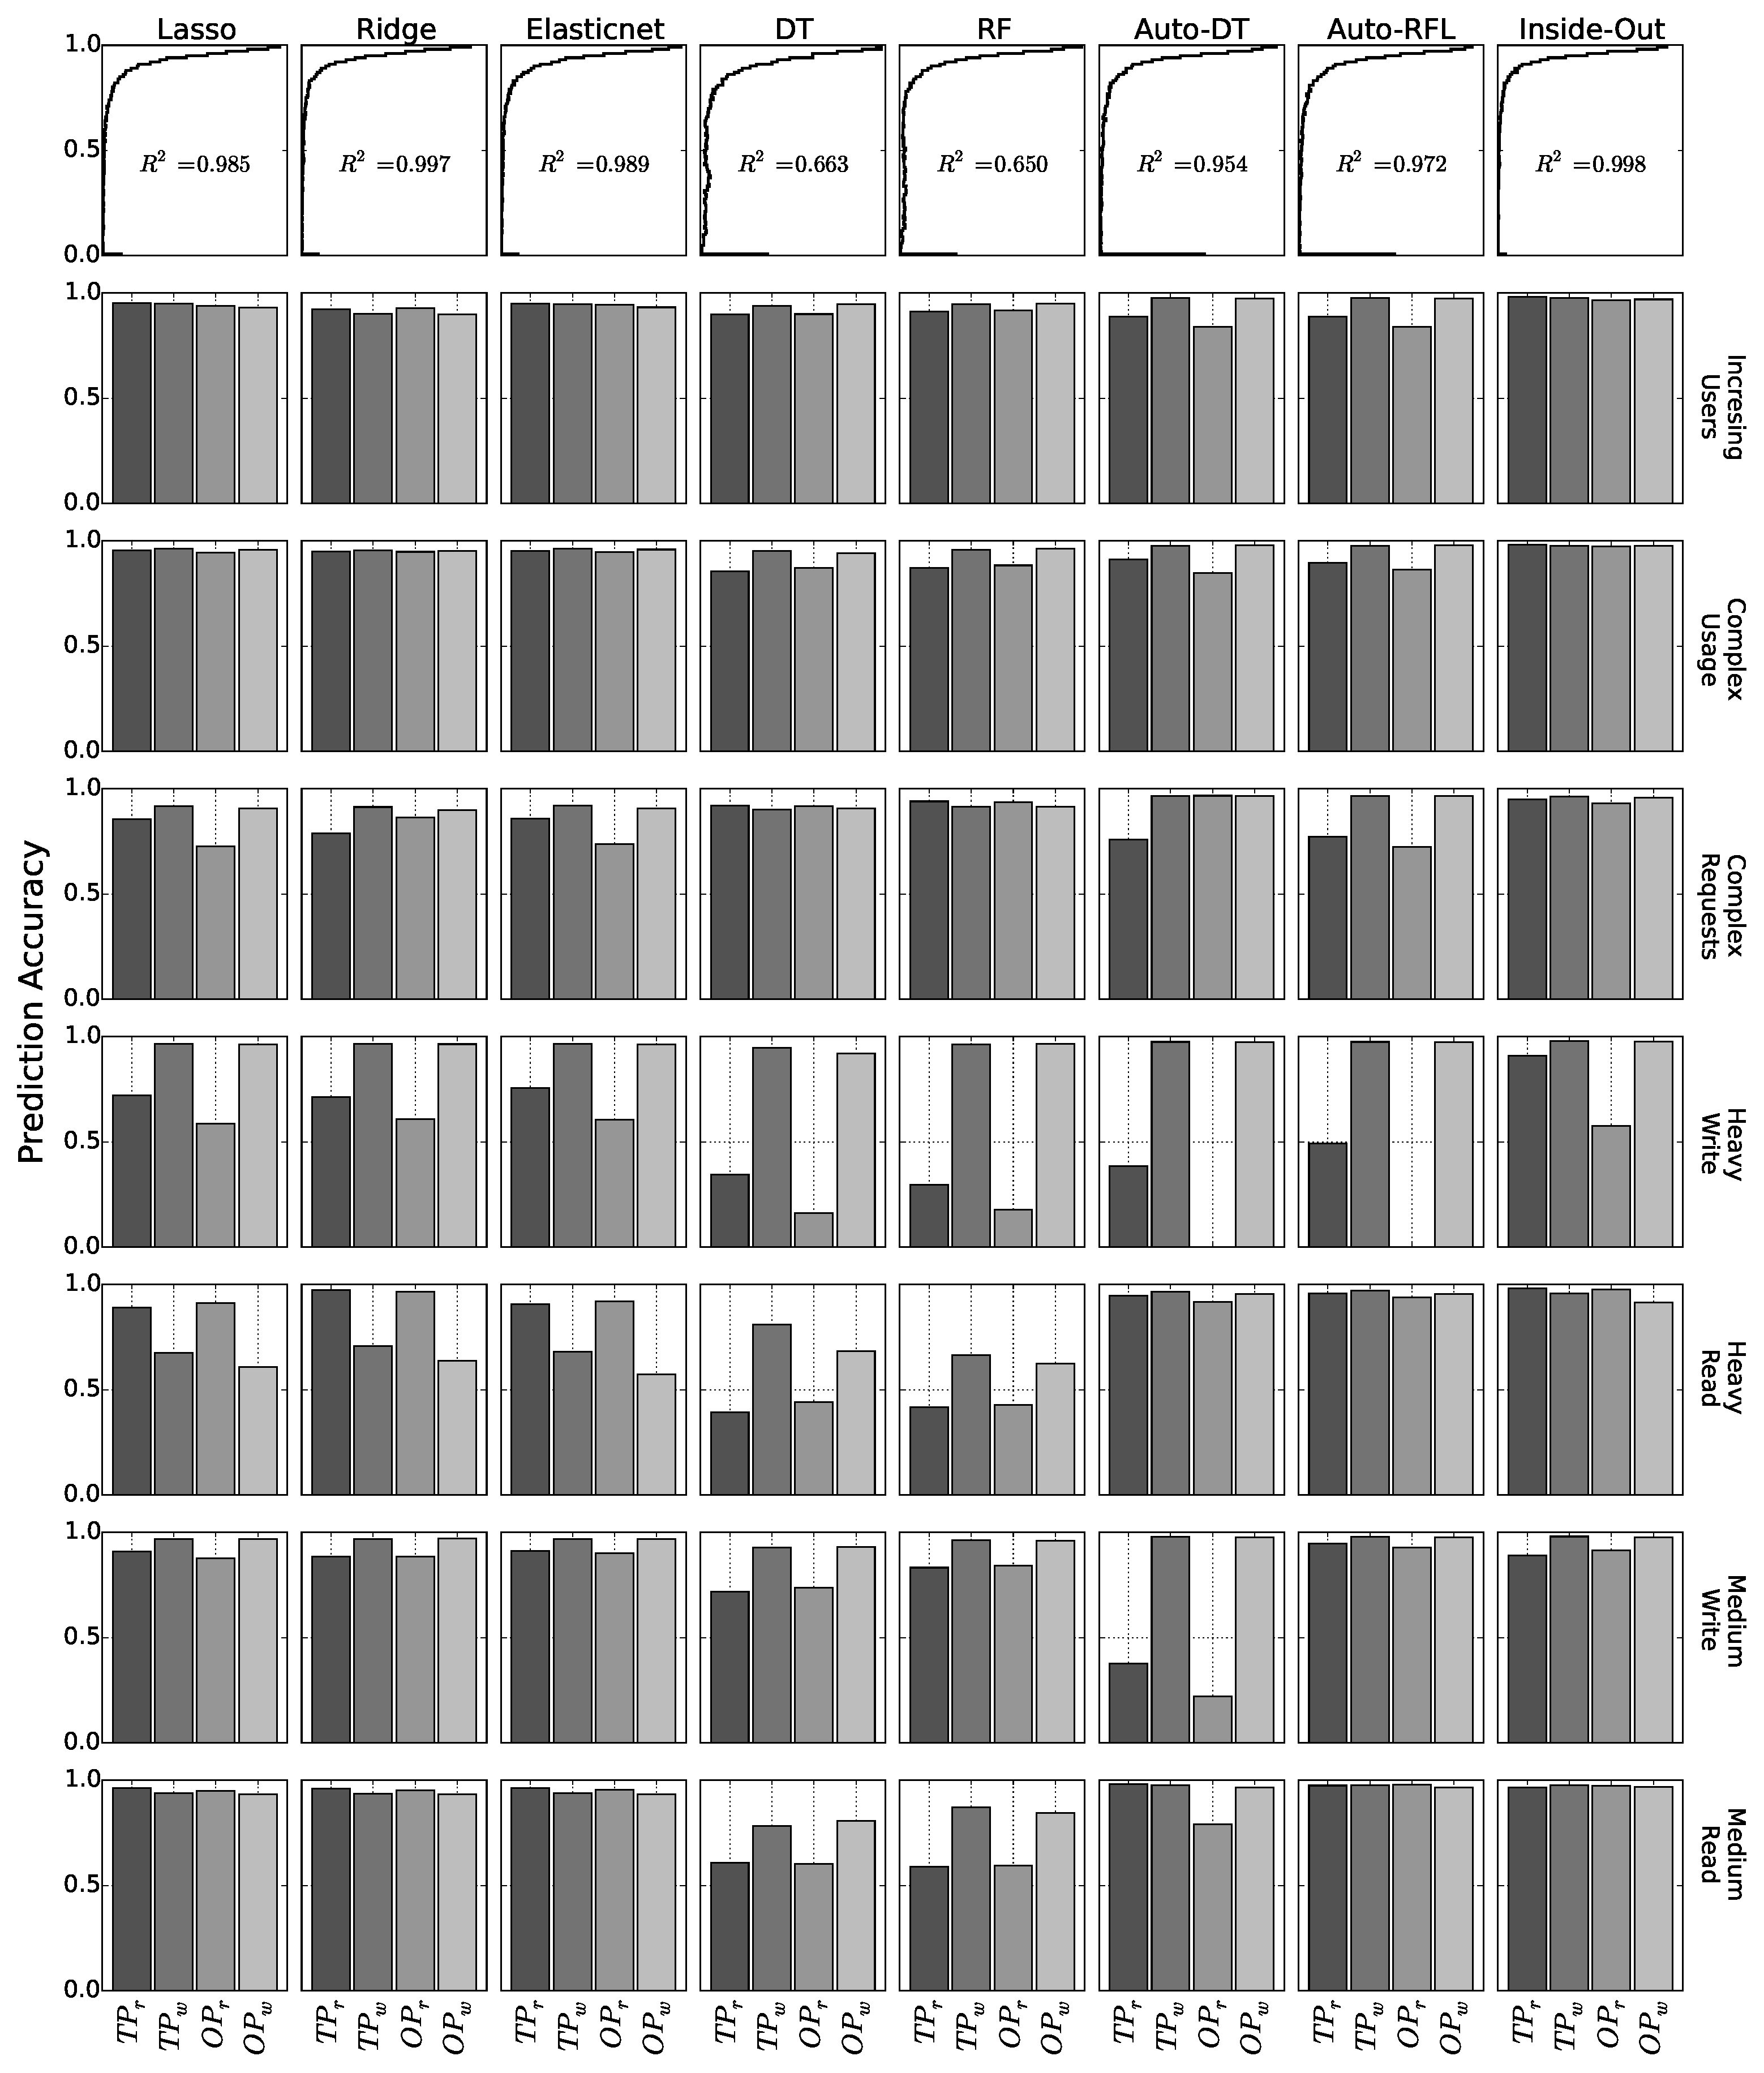
\includegraphics[width=0.9\textwidth]{Chapter-InsideOut/figures/unseen_workload_all_new.eps}
    \caption{Analysis of performance models with diverse workloads. Each bar is the average prediction accuracy. The top row is the probability density function of prediction accuracy for each performance model.}
    \label{fig:changing_workload}
\end{figure}

%\hfill\break

An SDS application needs to handle various request volumes, object/file sizes and different ratios of read/write workloads.
%In practice, it is difficult to obtain a training dataset that includes all access patterns.
First we examine whether Inside-Out can achieve accurate and consistent predictions when workload changes.


\paragraph*{Changing user behavior}
%\textbf{Changing user behavior.}

We increase the number of concurrent clients to stress the Ceph cluster.
%We push the Ceph cluster to a certain limit by increasing the parallelism of clients.
The \emph{\MakeLowercase{\scenarioMU}} scenario changes the number of COSBench clients and the \emph{\MakeLowercase{\scenarioCUB}} scenario increases the worker threads of each client.
As shown in \myfigure{\ref{fig:changing_workload}}, all prediction models perform well. The linear regression technique performs slightly better than the tree-based learning.
The linearly increasing load is well captured by linear models because of proportional change in low-level metrics.
When we switch to the \emph{\MakeLowercase{\scenarioCRB}} scenario, the variable request size slightly changes the behavior of Ceph, affecting prefetching and caching. 
We observe that the linear regression methods (Lasso, Ridge and Elastic Net) show drops in accuracy, e.g. 20\% in the $OP_r$ case; however, Inside-Out 
maintains good accuracy. 
The tree-based learning shows comparable predictions (5-10\% lower) with Inside-Out in these settings.



%\textbf{Complex request behavior.}
%Next, we change the workload from a constant IO request size to variable size.
%In this case, Inside-Out slightly improves the prediction accuracy over Lasso, %and outperforms the three linear models.
%Auto-DT and Auto-RFL show inconsistent prediction result with about 15\% %degradation of accuracy, comparing with the best case.
%One possible expalantion is that some important features filtered by DT and RF 
%are removed.
%Lasso and Elastic Net encounters accuracy drop in the read IOPS prediction


\paragraph*{Varying I/O pattern}

%The workload is a strong performance factor to a storage system \cite{Noorshams2013}.
%The read performance, for example, is affected by the amount of concurrent read or write operations.
Next, we consider workloads with different ratios of read to write operations.
\myfigure{\ref{fig:changing_workload}} shows that varying workload poses a big challenge to performance models. 
The linear regression methods (Lasso, Ridge and Elastic Net) present better prediction accuracy than tree-based models (DT, RL).
In addition, we observe that several models make poor predictions of $TP_r$ and $TP_r$.
The reason is that read behavior is largely affected by \textit{cache}, and large read variance contributes to low prediction accuracy.
Inside-Out performs consistently well, whereas the three linear regression techniques show accuracy drops.
One exception is the $OP_r$ prediction in the \textit{write-intensive} scenario even though $TP_r$ prediction is accurate.
As we will show later in Section~\ref{sec:online_learning}, \emph{over- and under-predictions} cause such behavior. 
The self-learning property of Inside-Out improves its prediction accuracy as it keeps learning the new storage behavior.


\begin{figure}
    \centering
    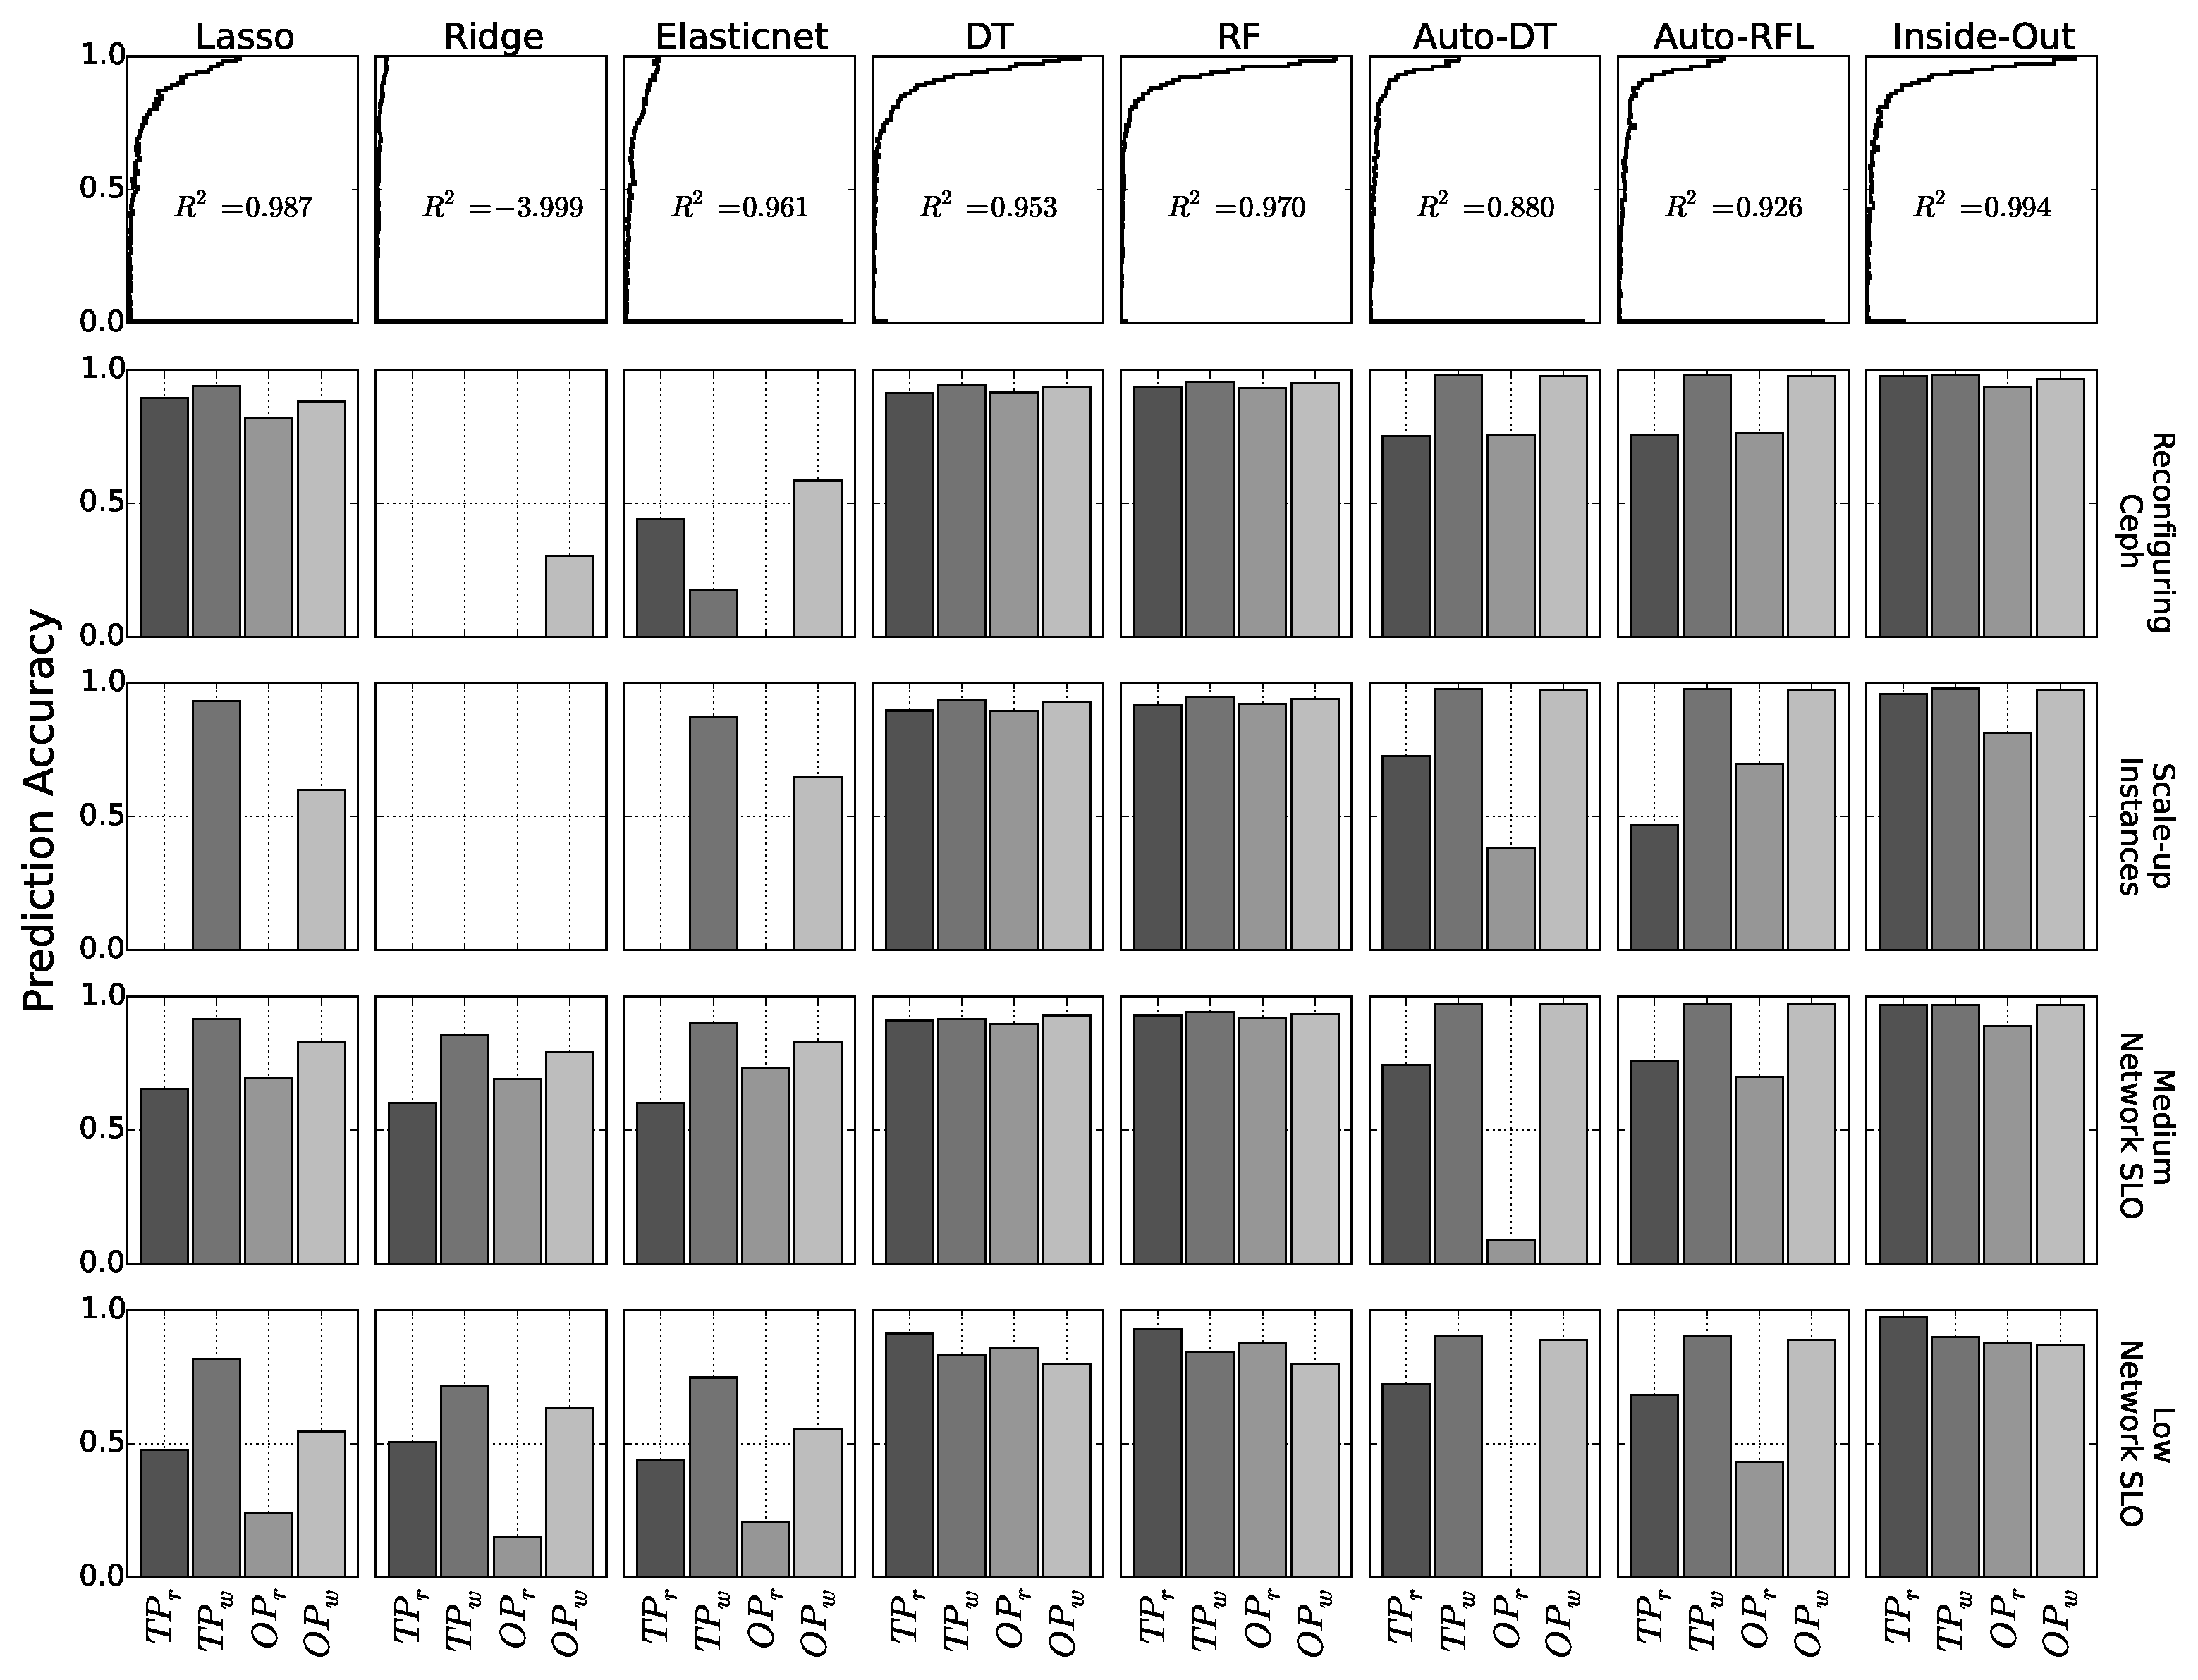
\includegraphics[width=0.9\textwidth]{Chapter-InsideOut/figures/unseen_configuration_all_new.eps}
    \caption{Comparison of performance models when the storage service is reconfigured: Ceph, VMs and network SLOs}
    \label{fig:reconfiguring_storage}
\end{figure}


\paragraph*{Summary}
The linear regression models achieve high prediction accuracy, great goodness-of-fit ($>0.98$) and consistency in prediction 
for many instances (see the distribution of prediction accuracy in \myfigure{\ref{fig:changing_workload}}), but they 
are not consistent across all prediction scenarios.
Inside-Out achieves good prediction accuracy across all cases consistently because the two-level approach 
filters out many irrelevant features in the first step, thereby presenting a smaller relevant feature space to the second step. 
The tree-based learning methods (DT and RF) do not show consistent prediction across all scenarios.
Auto-DT and Auto-RFL, which use DT and RF as the filter algorithms, are not as consistent as Inside-Out.

\vspace{1ex}

%\subsubsection{Reconfiguring Storage}
\subsubsection{Can Inside-Out handle different system configurations?}
\label{sec:unseen_configuration}

We study whether low-level metrics can capture the storage behavior when it is reconfigured by tenants. The results are reported in \myfigure{\ref{fig:reconfiguring_storage}}.


\textbf{Reconfiguring Ceph.}
The first change is to add one extra Ceph monitor daemon. %\chin{which increases the capability to handle a large number of clients.}
Ridge and Elastic Net fail to generate consistent predictions, but Lasso is able to achieve around 80\% to 90\% prediction accuracy.
DT, RF and Inside-Out have very close prediction accuracies, but Auto-DRL and Auto-RFL perform slightly worse in predicting $TP_r$ and $OP_r$.

\textbf{Scale-up instances.}
Increasing CPU and memory allocation to Ceph VM instances improves Ceph's ability to handle more requests.
In this test, we change the instance type from m1.small (1 vCPU, 2GB memory) to m1.medium (2 vCPUs, 4GB memory).
The linear models are unable to predict $TP_r$ and $OP_r$, but Inside-Out's two-level learning performs well by avoiding the overfitting problem. 

\textbf{Network SLOs.}
Here we consider the case where the amount of network bandwidth allocated to Ceph VMs is limited. 
We use Linux network throttling tool \textit{tc} to limit network bandwidth at 500 Mbps and 250 Mbps for medium and low bandwidth SLOs, respectively.
We observe that linear models without the two-level method do not show comparable prediction accuracy across both throughput and IOPS predictions.
The tree-based learning models, on the other hand, achieve 80\% to 90\% accuracy, comparable to Inside-Out.


\textbf{Summary.}
Tree-based learning (DT, RF) models demonstrate promising prediction in terms of prediction accuracy and consistency.
Lasso, Ridge and Elastic Net show inconsistent behavior in the above four scenarios.
Inside-Out, on the other hand, provides consistent predictions and improves Lasso, from 23.9\% to 87.6\% in the extreme case.


\begin{figure}
    \centering
    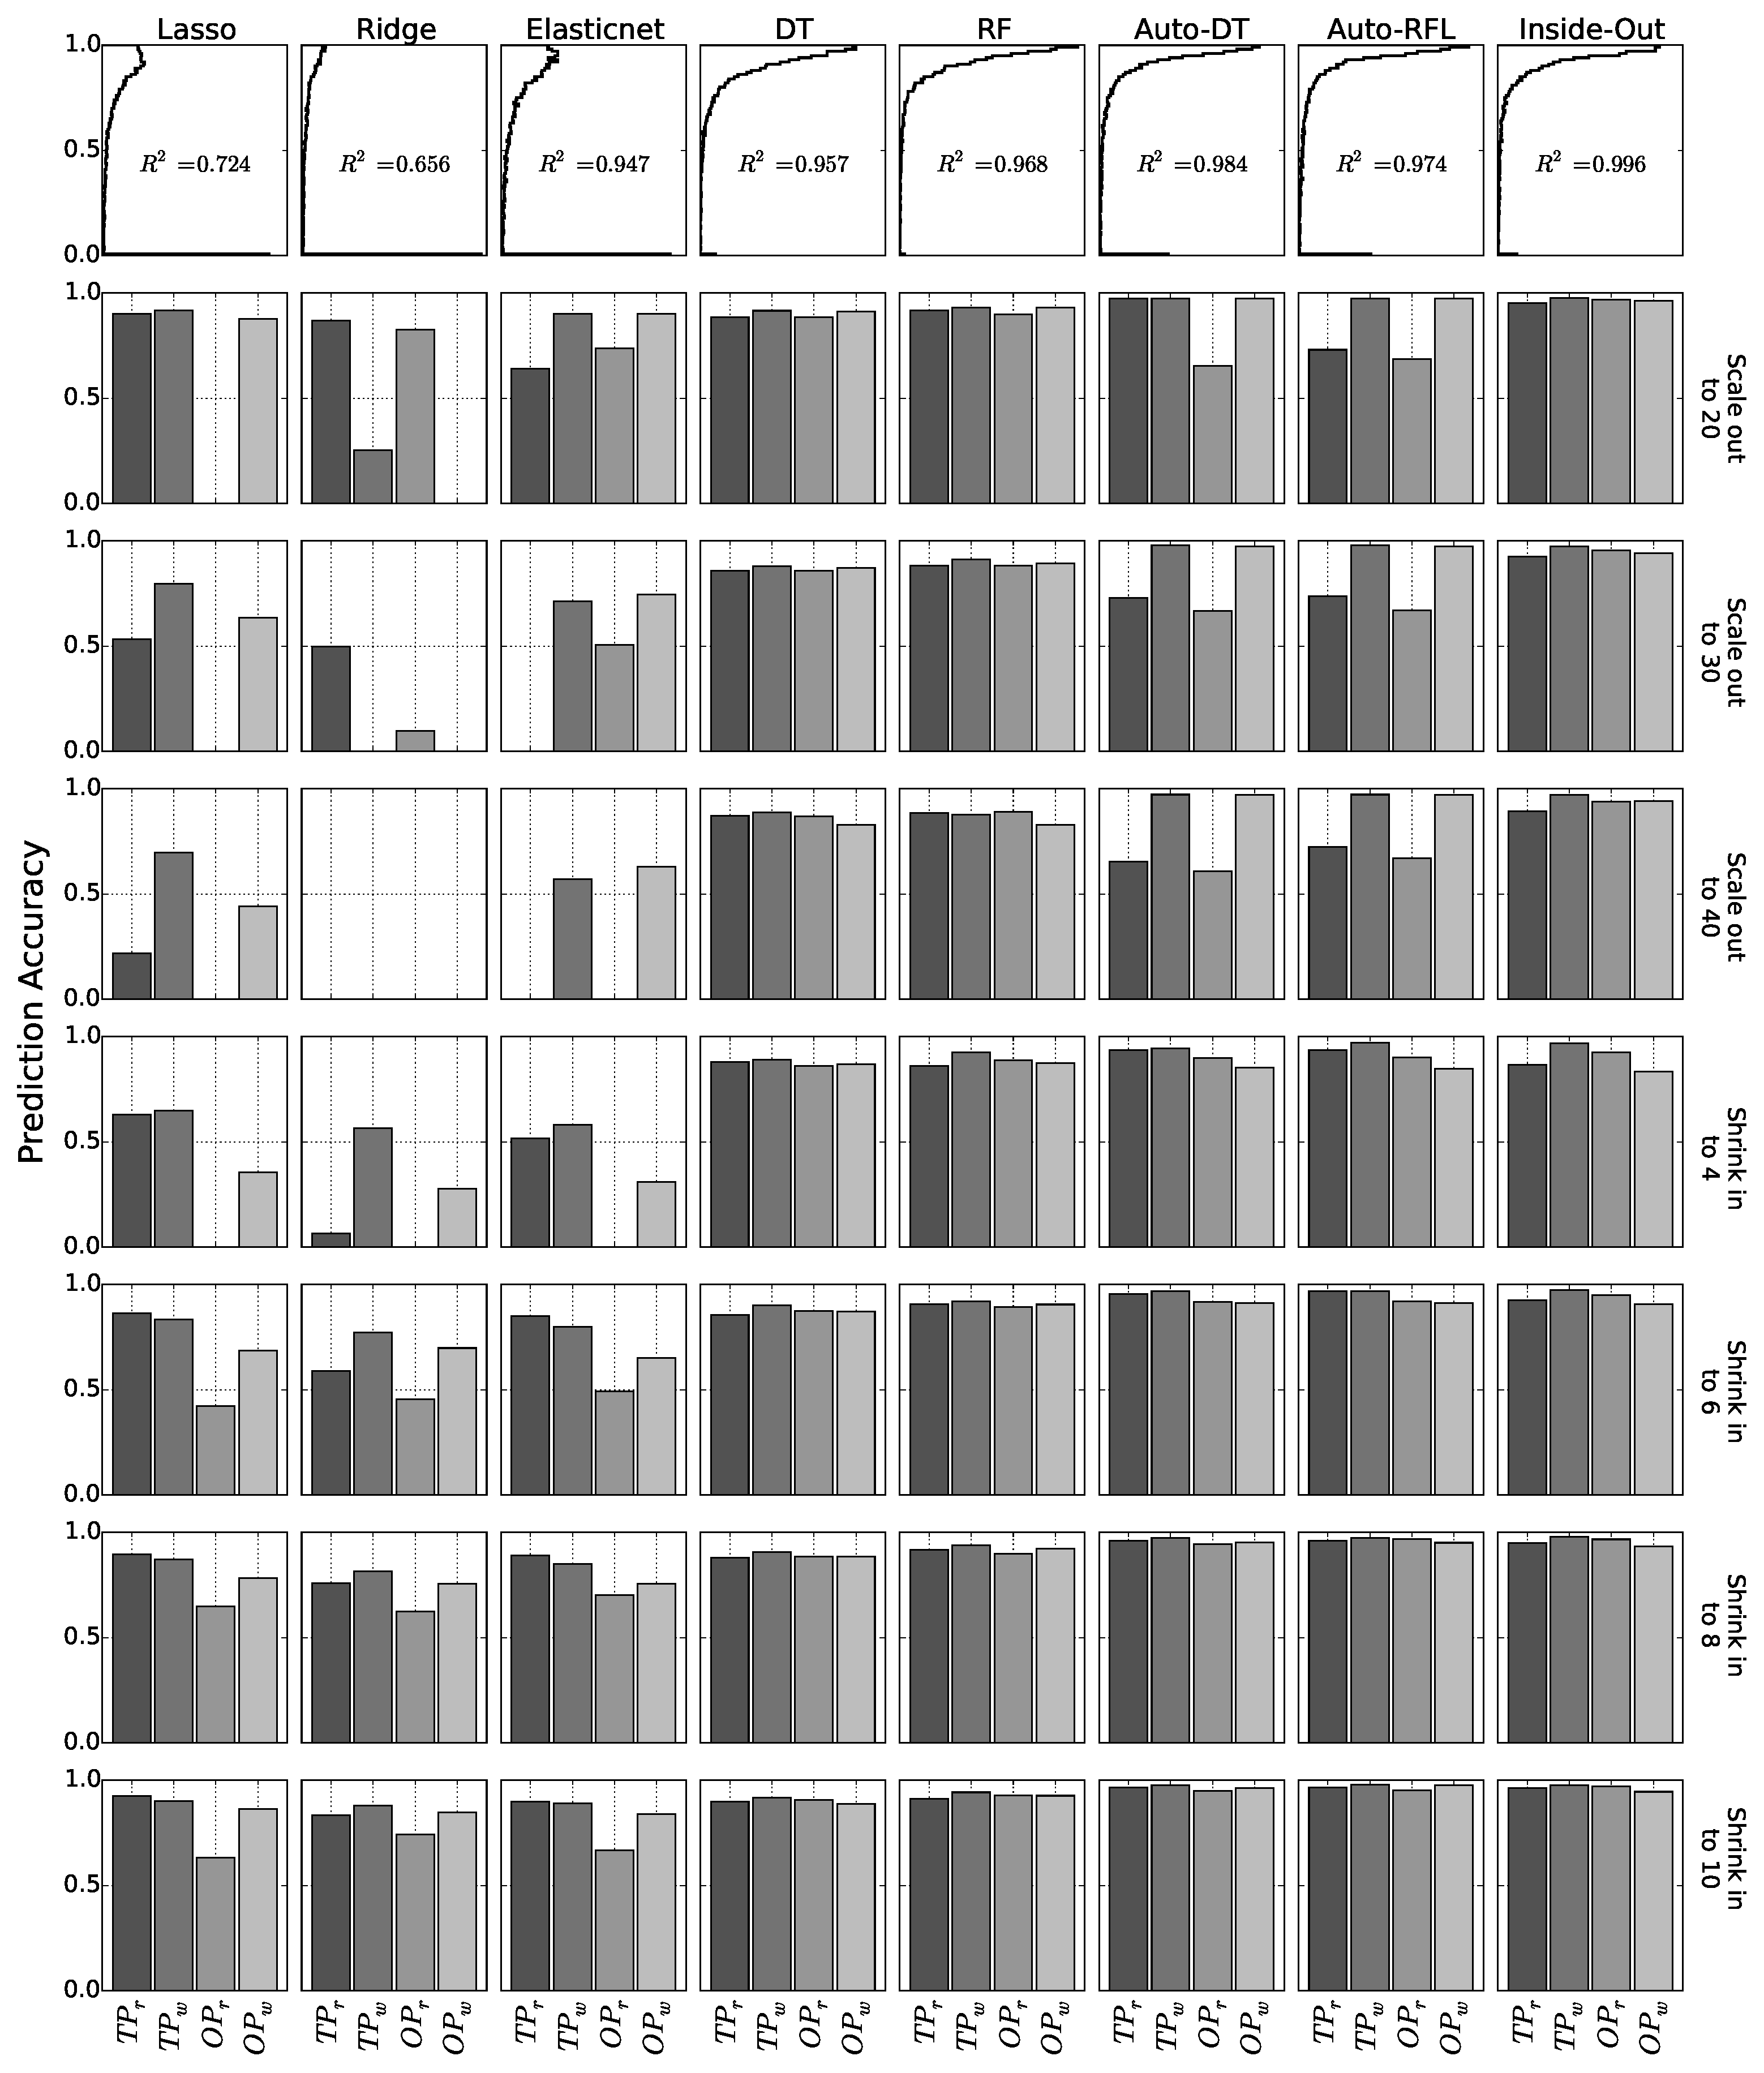
\includegraphics[width=0.9\textwidth]{Chapter-InsideOut/figures/unseen_scale_all_new.eps}
    \caption{Comparison of model performance in the on-demand scaling scenario. In the scale-out scenario, a performance model trained with 10 Ceph nodes is used to predict the performance of Ceph cluster with 20, 30 and 40 nodes.}
    \label{fig:elasticity}
\end{figure}


\subsection{Prediction Performance in a Multi-tenant Cloud}

This section examines the modeling performance of Inside-Out.
We first evaluate whether Inside-Out is able to extrapolate
performance of a larger Ceph cluster. 
Next, we evaluate how Inside-Out performs
when systems are subject to performance interference.

\subsubsection{Elastic Storage (On-demand Scaling)}
\label{sec:scaleout_prediction}

A storage service needs to grow or shrink its capacity on demand.
We evaluate Inside-Out's ability to capture the storage behavior at different system scales.
As shown in \myfigure{\ref{fig:elasticity}}, we use training data collected from 
4, 6, 8, and 10 nodes, and then predict the performance of 20, 30, and 40 nodes.
We also evaluate prediction accuracy in the \emph{shrink-in} scenario.
For both read and write throughput predictions, the linear models exhibit high variance.
In the $OP_r$ and $OP_w$ cases, the prediction results are not even comparable to the other methods.
Inside-Out, on the other hand, helps mitigate this issue, and achieves more than 90\% accuracy.
With increasing sizes of the storage, the prediction accuracy decreases because the prediction target 
becomes increasingly different from the training data.
Running a benchmark test against a very large system is time-consuming.
Here we demonstrate that Inside-Out can predict performance for systems that are 
four times larger than the system for which training data was collected.
%Due to resource limitations, we cannot show the upper bound of the largest system size that we can predict.
%However, we believe the upper bound can increase as the performance model keeps learning the system behavior.

\begin{figure}
    \centering
    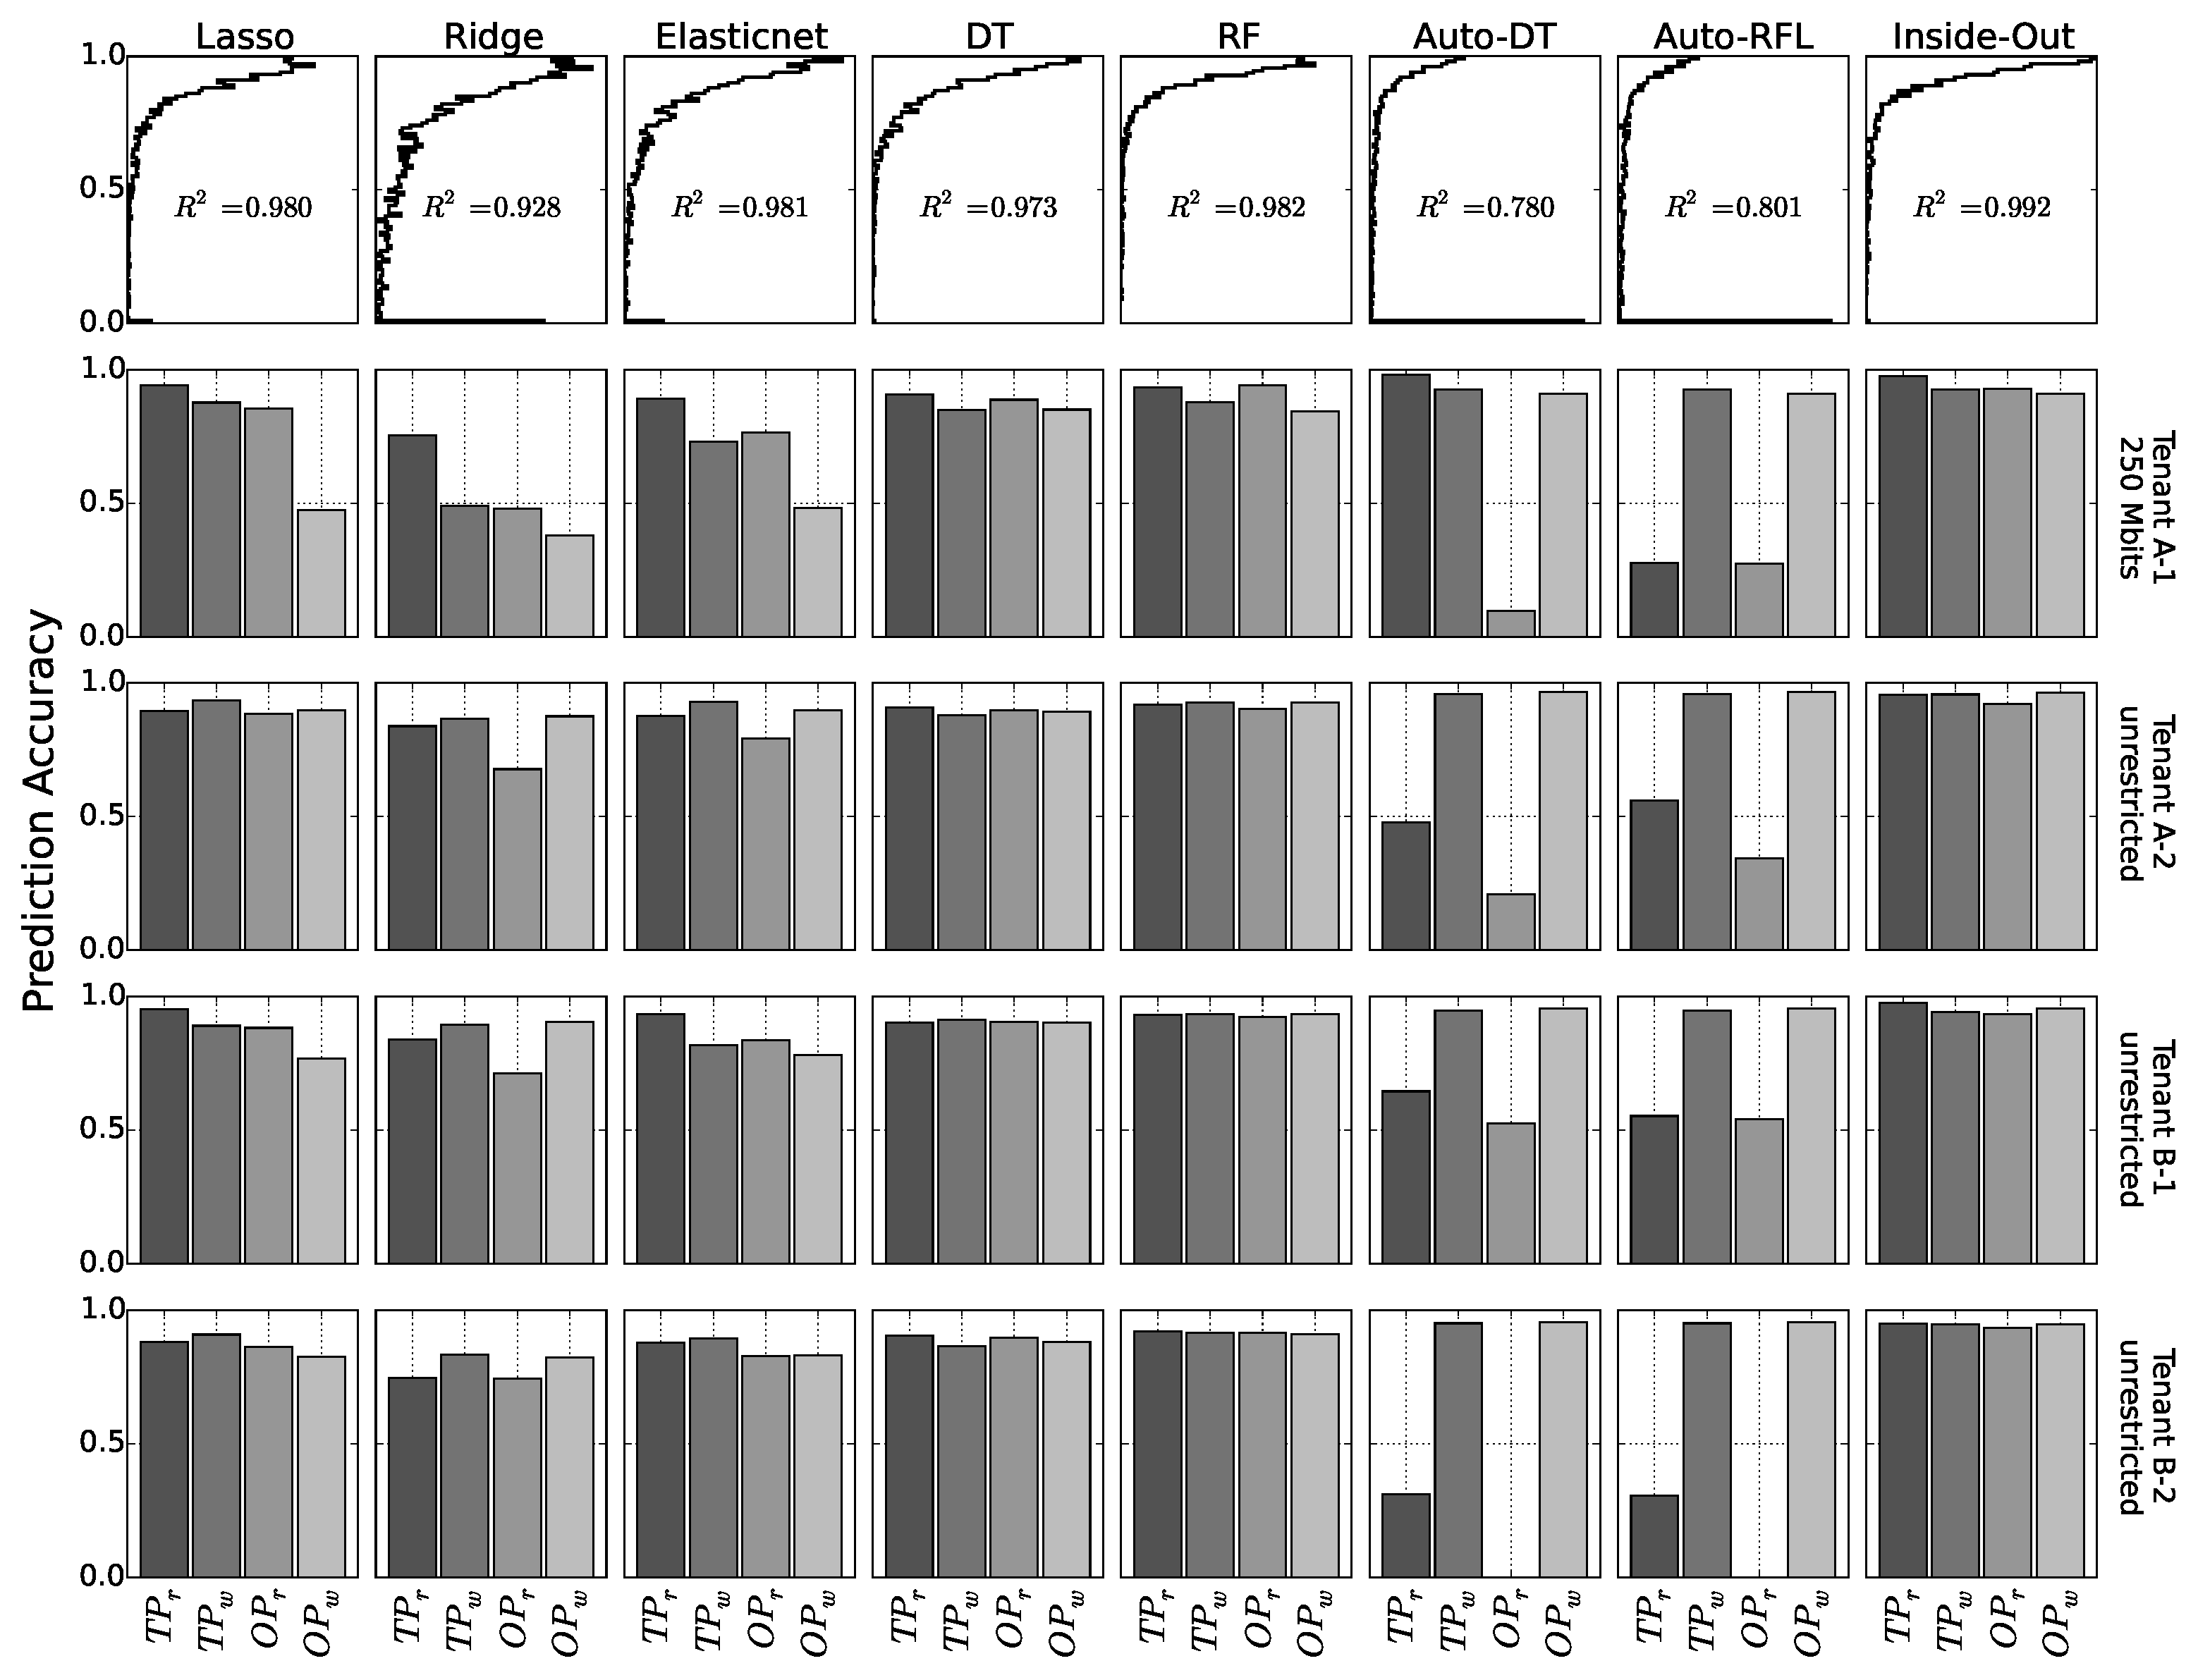
\includegraphics[width=0.9\textwidth]{Chapter-InsideOut/figures/multi_tenancy_all_new.eps}
    \caption{Prediction accuracy in a multi-tenancy scenario. Tenant A-1 is co-located with Tenant B-2. Tenant A-1 is throttled at 250Mbps. Tenant B-1 and B-2 are co-located without any traffic throttling.}
    \label{fig:multi_tenancy}
\end{figure}


\begin{figure*}
    \centering
    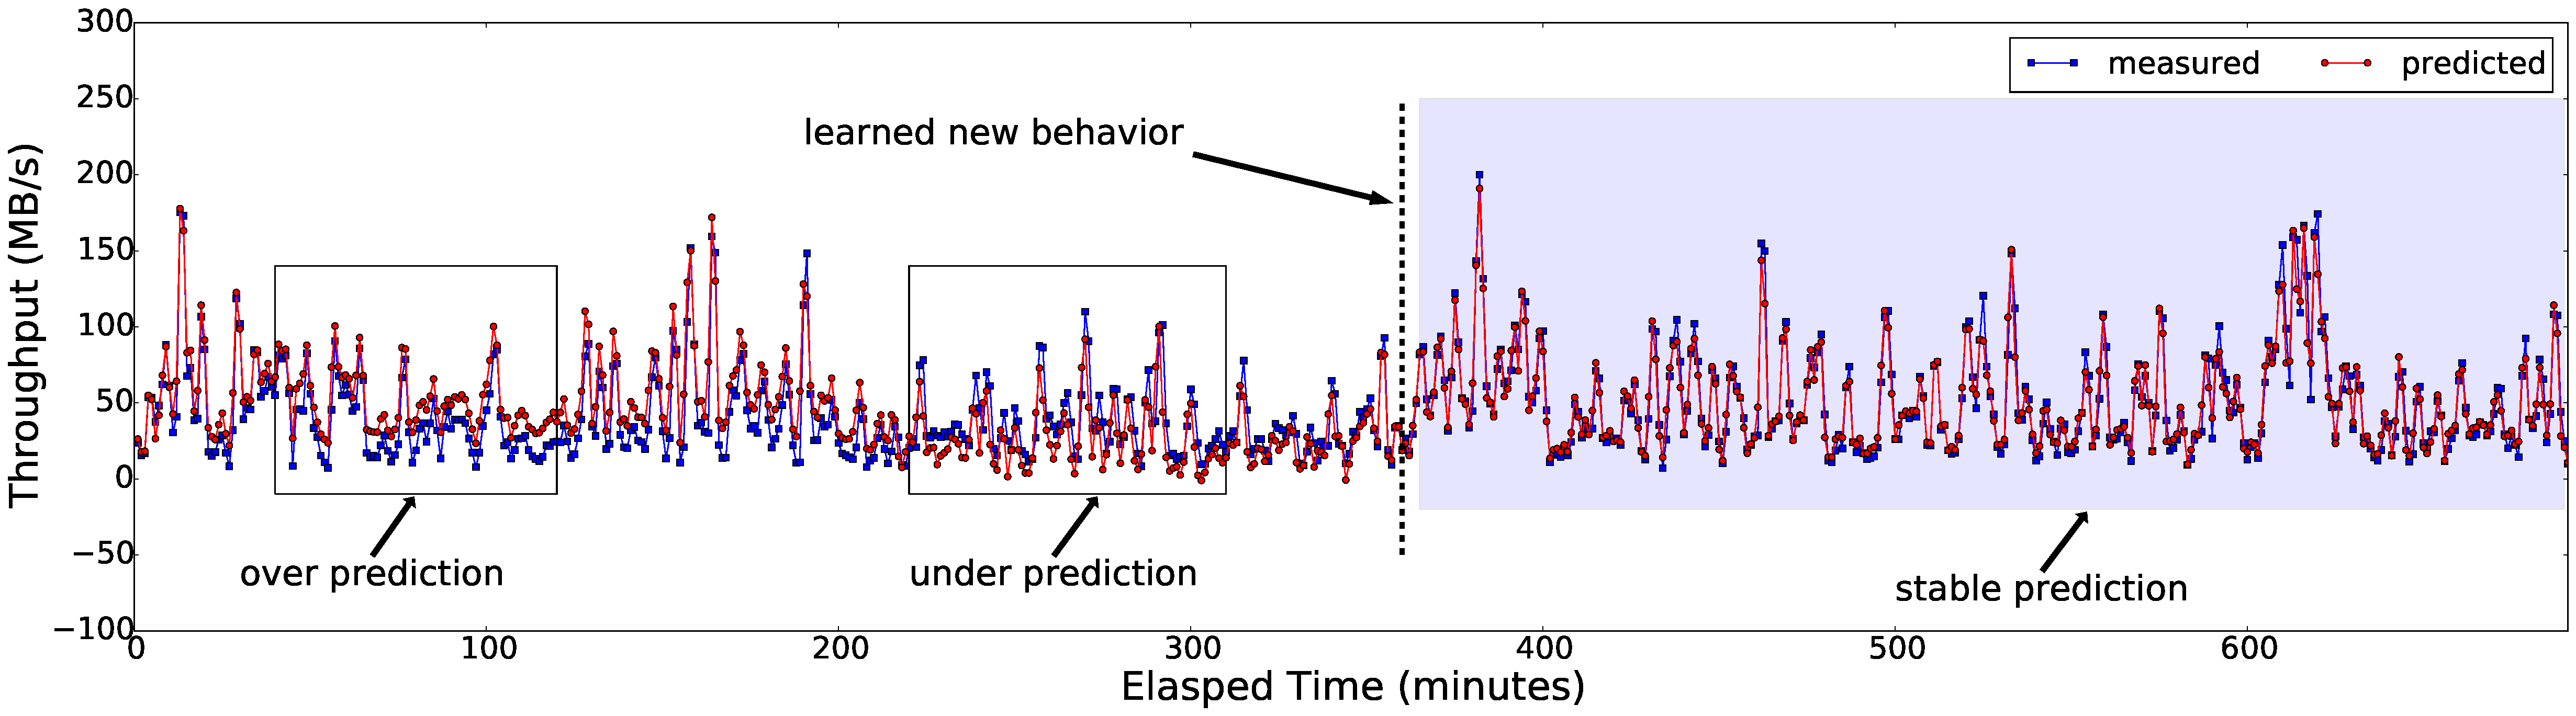
\includegraphics[width=0.9\textwidth]{Chapter-InsideOut/figures/real-world_tp_read.pdf}
    \caption{Application of Inside-Out to real time prediction of read throughput on a 10-node Ceph cluster.  Inside-Out starts from a simple prediction model trained by our collected benchmarking data.  Inside-Out keeps learning the storage behavior while improving prediction accuracy over time.}
    \label{fig:real_workload}
\end{figure*}


\subsubsection{Multi-Tenancy}
 
Next we evaluate Inside-Out's ability to adapt to performance interference among storage tenants.
We consider two cases for this evaluation. 
Each tenant runs a Ceph cluster with 10 OSDs separately, but tenants share the same 10 physical machines.
In the first case, we restrict the bandwidth of only the first tenant at 250Mbps.
%Two tenants compete for resources and \chin{\textbf{Tenant A-1}} has lower bandwidth SLO.
In the second case, we run two concurrent Ceph clusters but without network throttling.
\myfigure{\ref{fig:multi_tenancy}} shows that most prediction models are able to achieve more than 80\% accuracy.
The linear models like Ridge and Elasticnet yield lower prediction accuracies in some cases; however, Inside-Out performs well consistently.
Performance interference is challenging for a performance model designed for an isolated environment.
This evaluation demonstrates that the low-level performance metrics are good proxies for measuring
the end-to-end storage performance, even in a shared SDS environment.
%These metrics are able to reflect the behavior changes in the storage system.

%low-level performance feature selection approach is effective in capturing end-to-end performance, even under high storage interference.
%This property is important to SDS because it can help guarantee reliable end-to-end performance in a shared SDS environment.



\begin{comment}
\begin{figure*}
    \centering
    \includegraphics[width=0.9\textwidth]{figures/synthetic.eps}
    \caption{An online prediction scenario about six-hour long workload.  This synthetic workload is composed of 360 stages and each stage uniformly selects parameters such as workload types, request sizes and the number of clients.  The average stage duration is 60 seconds with standard deviation 20 seconds.}
\end{figure*}
\end{comment}

\begin{comment}
\begin{figure*}
    \centering
    \begin{subfigure}[b]{0.45\textwidth}
        \includegraphics[width=\textwidth]{figures/synthetic_read.eps}
        \caption{Read Throughput}
        \label{fig:synthetic_read}
    \end{subfigure}
    ~ %add desired spacing between images, e. g. ~, \quad, \qquad, \hfill etc.
      %(or a blank line to force the subfigure onto a new line)
    \begin{subfigure}[b]{0.45\textwidth}
        \includegraphics[width=\textwidth]{figures/synthetic_write.eps}
        \caption{Write Throughput}
        \label{fig:synthetic_write}
    \end{subfigure}
    \caption{An online prediction scenario about six-hour long workload.  This synthetic workload is composed of 360 stages and each stage uniformly selects parameters such as workload types, request sizes and the number of clients.  The average stage duration is 60 seconds with standard deviation 20 seconds.}
    \label{fig:synthetic_workload}
\end{figure*}
\end{comment}

%\subsection{Synthetic Workload}
\subsection{Online Self-Learning}
\label{sec:online_learning}

%Our goal is to apply Inside-Out to an online system so that SDS providers can guarantee the performance of a storage service hosted on their SDS platform.
%To evaluate this potential, 
Next, we create several synthetic workloads with mixed read/write ratios.
This synthetic workload spans 12 hours with 720 stages.
Each stage is 60-second long on average, with a standard deviation of 20 seconds.
We run four COSBench virtual machines for benchmarking and up to eight threads per COSBench client, with 10 Ceph OSDs and one monitor daemon.
We use Inside-Out to build an initial performance model with the training dataset described in Section~\ref{sec:dataset}.
\myfigure{\ref{fig:real_workload}} shows the prediction result for read throughput.
We can observe that the generated model can capture the overall trend, but suffers from over and under predictions.
This is because our training dataset is generated from a relatively clean environment, \ie the OS memory is flushed before any benchmarking process.
However, in the online prediction setting, cache is continuously consumed by non-stop client requests, which 
causes the real time storage behavior to be different from the training dataset.
With continuous monitoring of the performance of the storage service, 
we use Inside-Out to generate a new performance model at the sixth hour.
\myfigure{\ref{fig:real_workload}} shows that Inside-Out learns the new storage behavior and therefore, 
the over- and under-prediction issues are greatly mitigated.
%This evaluation demonstrates the potential of Inside-Out when applying it in an online system.
By continuously learning the storage behavior, SDS can accurately capture performance changes and therefore is able to provide reliable storage service.

%the problems due to over- and under-predictions are greatly mitigated.
%This evaluation demonstrates how Inside-Out can be used to continuously learn the storage behavior in an online system.


\begin{figure}
\centering
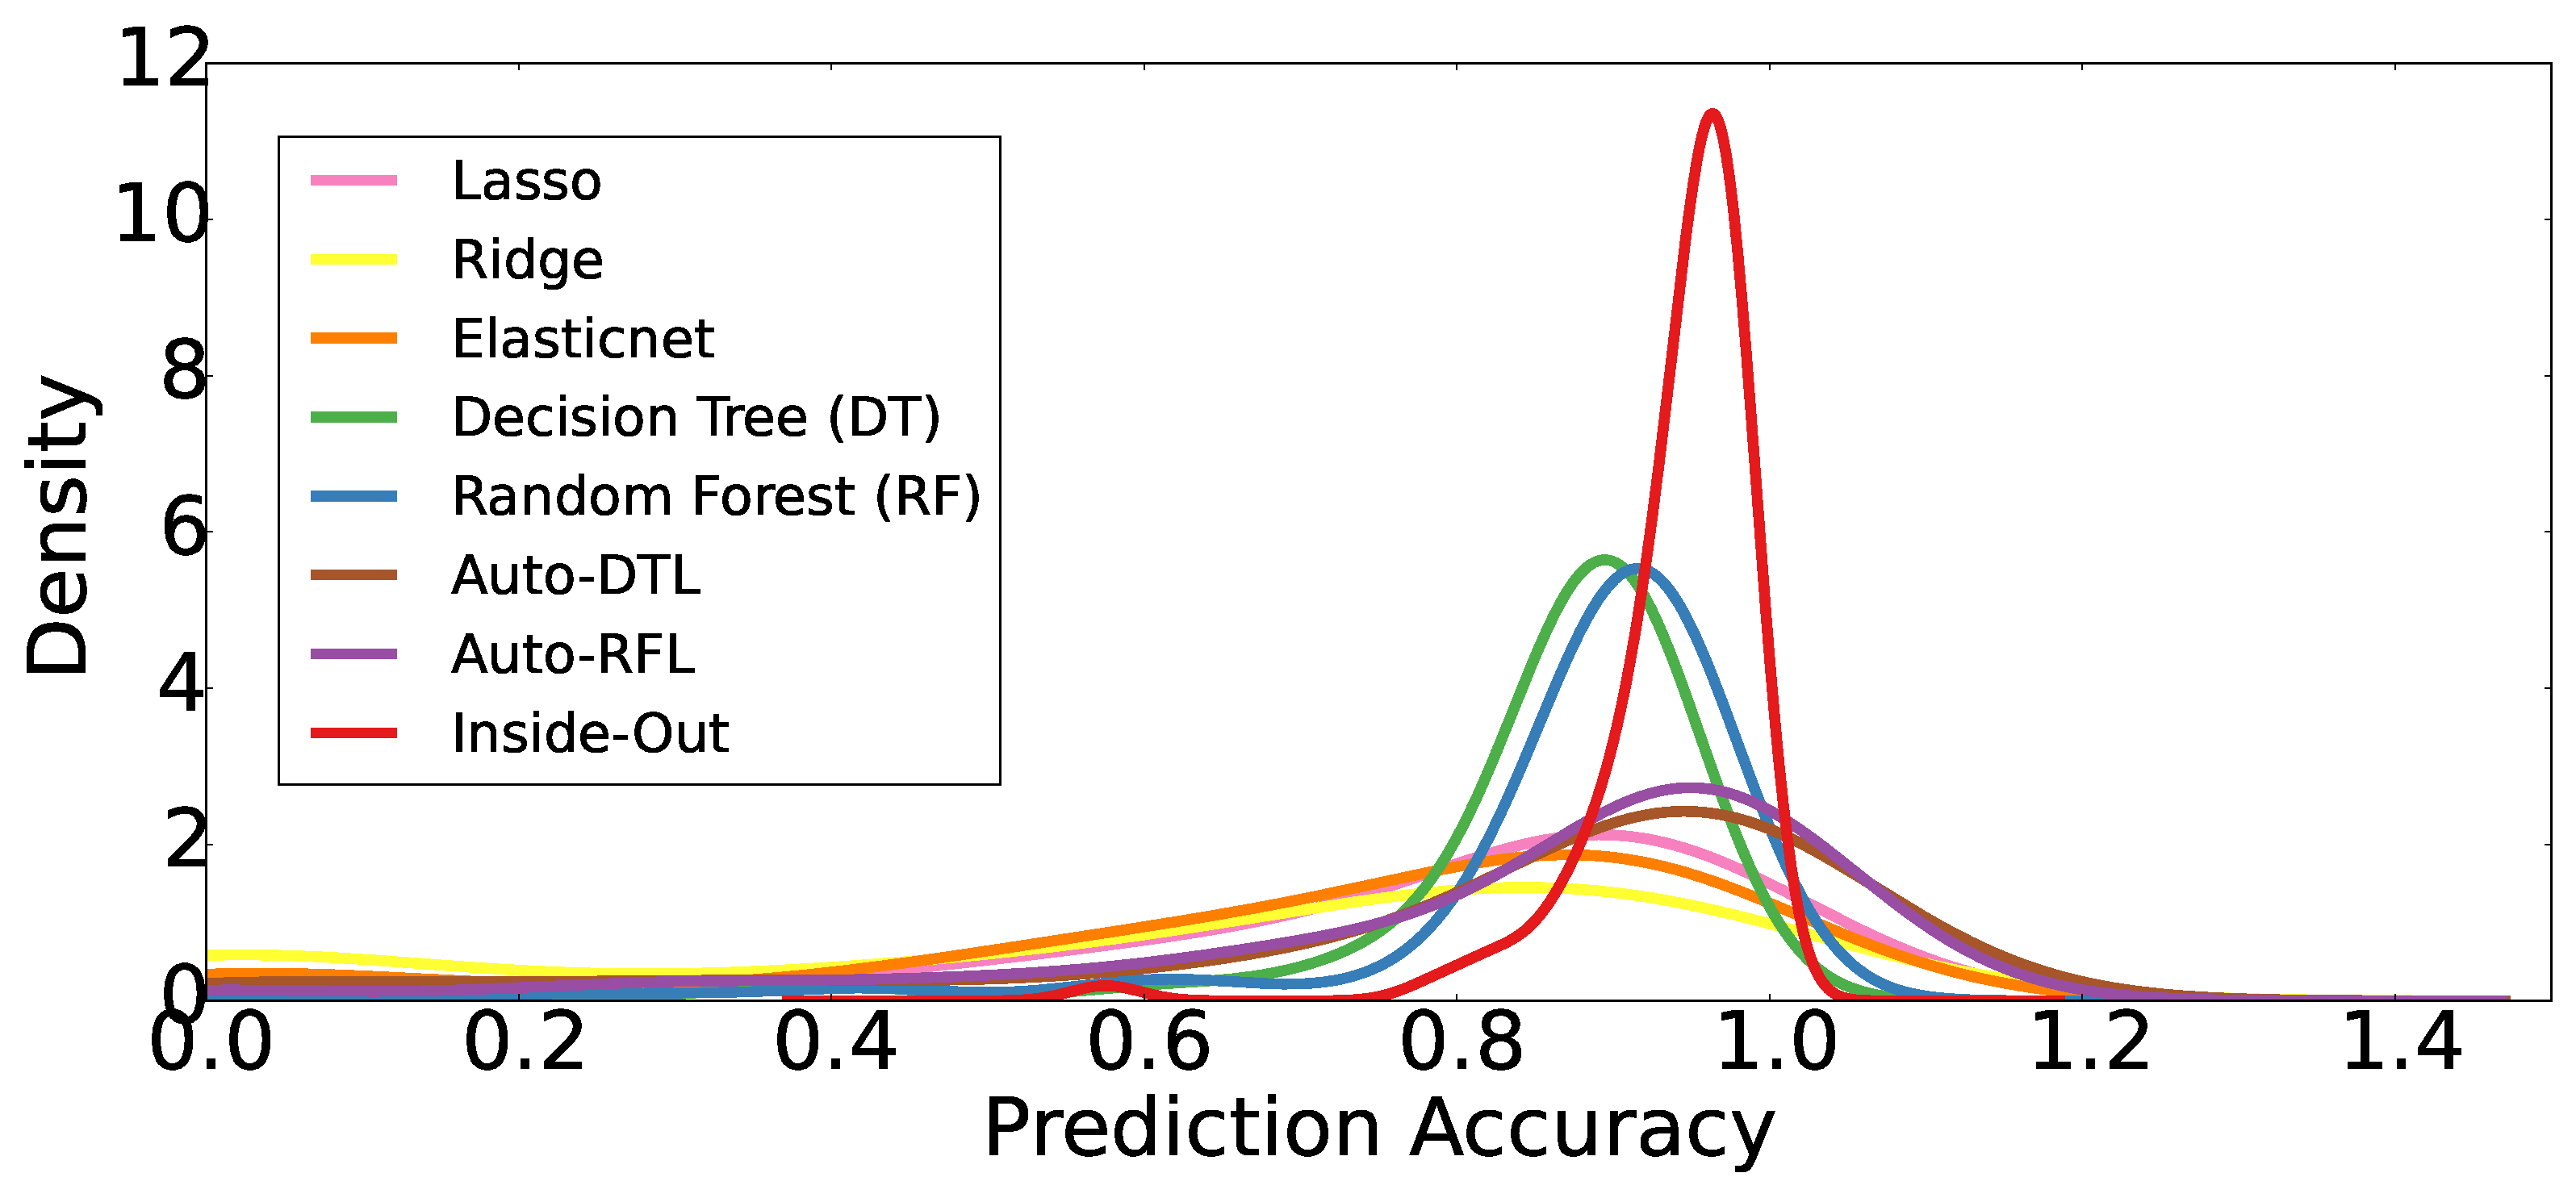
\includegraphics[width=0.9\textwidth, keepaspectratio]{Chapter-InsideOut/figures/aggregate_median.eps}
\caption{Kernel density function of prediction accuracy from \myfigure{\ref{fig:changing_workload}} to \myfigure{\ref{fig:multi_tenancy}}.  Each colored line represents the density function of a modeling approach.  Inside-Out is more consistent and accurate across almost every prediction case.}
\label{fig:aggregate}
\end{figure}


\vspace{1ex}
\subsection{Discussion}
We have shown that low-level performance metrics are useful to predict end-to-end throughput and IOPS.
%We applied Inside-Out to latency prediction and observe large variance and inconsistency.
%\chin{One} possible explanation is insufficient features and high variance in latency.
%The \chin{collected} low-level metrics are related to utilization, and these metrics might not provide enough information to fit a good model for predicting latency.
%Common approaches usually require request-level information \cite{Wang2004}.
%We need to further investigate latency prediction with other alternative generic low-level performance metrics.
Our evaluation has shown that low-level performance metrics are good indicators of end-to-end throughput and IOPS. 
Most existing performance models exhibit an inconsistent prediction behavior in the presence of diverse storage scenarios, 
such as changing workload, storage reconfigurations,
growing/shrinking storage, and multi-tenancy environments.
Our proposed two-level learning method can greatly improve prediction accuracy and yield consistent behavior.
Machine learning provides powerful tools, but they need to be used intelligently to achieve the best prediction accuracy. 
\myfigure{\ref{fig:aggregate}} shows the kernel density function of prediction accuracy across all prediction scenarios.
Inside-Out is a clear winner in terms of accuracy and consistency. 
More importantly, Inside-Out is able to learn new storage behavior, thereby enabling the performance model to adapt to the complex SDS environment.





%\section{Related Work}
\label{ch4:sec:relatedwork}

Storage performance modeling has been extensively explored in many prior works. 
Three common modeling techniques are analytical, simulation and data-driven approaches \cite{Shriver1998, Kelly2004, Ardagna2014}.
The analytical (mathematical) model requires domain knowledge to manually identify the factors that affect performance\cite{Shriver1998, Kelly2004}.
Kelly et al. use a probability model to predict response time for an enterprise storage array.
Ruemmler et al. found that a disk is too complex to model with analytical methods and designed a disk simulator to characterize storage behavior \cite{Ruemmler1994}.
However, the simulation approach becomes inefficient when searching a large design space \cite{Kelly2004}.


The data-driven or the measurement-based approach
uses measurement data to derive a prediction model. 
Wang et al. \cite{Wang2004} adopt classification-and-regression-tree (CART) to predict the response time of a single disk and a disk array.
The authors propose request-level and workload-level device models for different prediction granularities.
Yin et al. also use the regression tree to predict storage throughput and latency \cite{Yin2006}.
Their work mainly focuses on multiple workloads, and proposes a scalable model, by combining related workload features.
Noorshams et al. extensively analyze four different types of algorithms 
(including linear regression and CART models) and apply to IBM storage servers \cite{Noorshams2013}.
They also propose an optimization technique to search for parameters that can improve prediction accuracy.
Their proposed parameter optimization complements our work for improving prediction accuracy.
To sum up, Inside-Out uses only low-level performance metrics and does not require workload profiles and storage configurations.
Unlike these studies, Inside-Out is primarily designed for diverse storage services that need to be reconfigured frequently to meet users' demand. 


Mesnier et al. \cite{Mesnier2007} propose a novel black-box approach that can describe the performance difference between two storage devices.
It may be possible to borrow this idea and apply it to the unseen configuration scenarios as described in Section \ref{sec:unseen_configuration}.
With this approach, we can study the performance difference between two configurations and create a combined model with better prediction accuracy.
Bodik et al. propose an exploration policy for quick collection of essential data required to train a performance model \cite{Bodik2009}.
This policy can reduce the time required for offline and online model training.


Chen et al. propose SLA decomposition that combines profiling and queuing model to derive resource thresholds for meeting application SLA \cite{Chen2007}.

%SLA decomposition is used to determine the resource threshold that can meet a certain SLO \cite{Chen2007}.
%In \cite{Chen2007}, the authors propose using component profiling to build a queuing network model for predicting end-to-end performance. 
%Our black-box approach does not require domain knowledge.
%Their work focuses on three-tier web applications and our focus is to create accurate performance models for software-defined storage.
%Moreover, we consider more realistic cases such as unseen workload, different configurations, resource interference and varying cluster sizes.
%% to add
%% \cite{Madhyastha2012}

Machine learning has also been applied to performance modeling for virtual machines (VMs).
DeepDive uses the classification technique to detect performance anomaly among VMs \cite{Novakovic2013}.
In \cite{Kundu2010}, the authors apply regression and artificial neural network to model performance of a single VM.
Our work focuses on performance prediction of a distributed storage system that includes multiple software and hardware entities.

\section{Conclusion}
\label{sec:conclusion}

Ensuring end-to-end performance in software-defined storage (SDS) requires accurate performance models. This chapter presents Inside-Out, a tool that provides reliable and consistent prediction of end-to-end performance of distributed storage systems using low-level system metrics. Our evaluation indicates that Inside-Out is able to generate accurate prediction models even when the storage environment differs significantly from the training phase. Inside-Out is generic in nature because it does not use application or protocol specific data for building performance models. Although we used Ceph as an example distributed storage service to evaluate Inside-Out, we believe it should be applicable to other storage systems as well with minor modifications.

\chapter{Cloud Architecture Tuning}
\label{chapter:cat}

This chapter formulates the problem of cloud architecture tuning (CAT) and describes the challenges in CAT with large-scale evaluation conducted on AWS.

\section{Introduction}
\label{sec:cat::introduction}

\iffalse
Cloud computing is a cost-effective
alternative to on-premise computing.
Cloud computing (specifically, Infrastructure as a Service) provides a large variety of architectural configurations,
such as the number of cores, amount of memory, and the number of nodes.
Cloud service providers
(such as Amazon, Google, and Azure) offer over 100 virtual machines (VM) types~\cite{Yadwadkar2017}.
The ready flexibility in cloud offerings has created a paradigm shift.
Whereas before a workload was tuned for the cluster that was available, in the cloud
the \emph{architectural configuration can be tuned for the workload}.
This flexibility imposes a burden on users who must choose the \emph{right} architectural configurations.
The wrong choice can increase elapsed time by 20 times and 
cost 10 times compared to the optimal~\cite{Hsu2018Arrow,Hsu2018Scout}.
Users need an effective way to find the right architectural configurations
for their cloud applications.
Therefore,
choosing the right VM type for a workload is essential to provide quality service while being cost effective~\cite{Frey2013, Yao2017}.
\fi


Cloud computing is a cost-effective alternative to on-premise computing.
Choosing the right VM type for a workload is essential to provide quality service
while being cost effective~\cite{Frey2013, Yao2017}.
In this chapter, we describe the \emph{cloud architecture tuning (CAT)} problem
~\cite{Venkataraman2016,Alipourfard2017,Yadwadkar2017,Hsu2018Arrow}.
Given a workload and a service objective, we focus on delivering
the best architecture configurations, such as
virtual machine (VM) types and the number of VMs.
CAT is similar to hyper-parameter tuning in many aspects
~\cite{herodotou2011starfish,zhu2017bestconfig,Dewancker2015,shahriari2016taking,Klein2017,golovin2017google}.
However, the search space of CAT can be more irregular,
which makes existing approach to CAT more fragile~\cite{Hsu2018Arrow}.
This is because the same workload can perform very differently
on two similar configurations.
For example, memory bottleneck can exist in one configuration but not another.

A good solution for CAT should have 
low search cost and find (near) optimal configurations.
Additionally, the solution should be reliable, scalable, and work for wide range of applications and workloads.
\emph{Ernest} is an effective method to extrapolate workload performance
on different configurations, but it is not scalable because
it requires separate prediction models
for distinct workloads and VM types~\cite{Venkataraman2016}.
\emph{CherryPick} adopts Bayesian Optimization to support
any kinds of workloads~\cite{Alipourfard2017}.
However, it relies on an appropriate kernel function to model the search space,
which makes it fragile~\cite{Hsu2018Arrow}.
\emph{PARIS} uses extensive training data
to build prediction model~\cite{Yadwadkar2017}.
However, it may suffer from a high variance of prediction error.
Thus, no prior work fulfills all the requirements of a good solution.
\section{Open Performance Data}
\label{sec:cat::dataset}

To evaluate a \cat method,
we need large-scale performance dataset---evaluating diverse workloads on different architectural choices.
We conducted a large-scale evaluation using different workloads and software systems on Amazon Web Services (AWS)~\cite{aws}.
We choose Apache Hadoop (version 2.7) and Apache Spark (version 1.5 and 2.1) as our software system~\cite{hadoop, spark}.
Our evaluation includes data processing, OLAP queries, and machine learning, which are popular applications on Hadoop and Spark.
We choose 18 VMs and run the 30 applications on them. \mytable{\ref{tab:dataset}} lists all the software systems and
applications.



\begin{table}[!htbp]
\centering

\caption{The evaluated applications. In total, there are 30 applications and 107 workloads measured on Hadoop 2.7, Spark 1.5 and Spark 2.1.}
\label{tab:dataset}
\resizebox{.95\linewidth}{!}{%
\begin{tabular}{@{}p{2.5cm}p{14cm}@{}}
\toprule
\textbf{Application} & \textbf{Description} \\ \midrule
\multicolumn{2}{l}{\noindent{\textbf{Micro Benchmark}}} \\
sort & Sorts text input data, generated by RandomTextWriter in Hadoop. \\
terasort & A standard Hadoop benchmark. Data is generated from TeraGen. \\
pagerank & The PageRank algorithm. Hyperlinks follow the Zipfian distribution. \\
wordcount & Counts the frequency of words that generated by RandomTextWriter.  This is a typical MapReduce job. \\ \midrule
\multicolumn{2}{l}{\textbf{OLAP}} \\
aggregation & A Hive query performing aggregation. \\
join & Implement the join operation in Hive \\
scan & Implement the scan operation in Hive \\ \midrule
\multicolumn{2}{l}{\textbf{Statistics Function}} \\ 
chi-feature & Chi-square Feature Selection. \\
chi-gof & Chi-Square Goodness of Fit Test. \\
chi-mat & Chi-square Tests for identity matrix. \\
spearman & Compute Spearman's Correlation of two RDDs. \\
statistics & Generate column-wise summary statistics. \\
pearson & Compute the Pearson's correlation of two series of data. \\
svd & Singular Value Decomposition, a fundamental matrix operation for finding approximate solutions.\\
pca & Principal Component Analysis for dimension reduction. \\
word2vec & Generate distributed vector presentation of words according to distance. \\ \midrule
\multicolumn{2}{l}{\textbf{Machine Learning}} \\
classification & Implement the generalized linear classification model. \\
regression & Generalized Linear Regression Model. \\
als & The Alternating Least Squares algorithm, implemented in spark.mllib. It is a collaborative filtering algorithm used for product recommendation. \\
bayes & Implements the Naive Bayes algorithm for the multiclass classification problem. Input documents are generated from /usr/share/dict/linux.words.ords. \\
lr & A popular algorithm for the classification problem. \\
mm & Matrix multiplication with configurable row, column and block sizes.\\
d-tree & A greedy algorithm for classification and regression problems. \\
gb-tree & Gradient Boosted Tree, an ensemble learning method for classification and regression problems. \\
df & The Random Forest algorithm for classification and regression problems. \\
fp-growth & The FP-growth algorithm to mine frequent pattern in large-scale dataset. \\
gmm & Gaussian Mixture Model is a clustering algorithm that uses k Gaussian distributions to find the k clusters. \\
kmeans & K-means is a common clustering algorithm that finds k cluster centers. \\
lda & Latent Dirichlet allocation is a clustering algorithm that infers topics from a collection of text documents. \\
pic & Power iteration clustering is a scalable algorithm for clustering. \\ \bottomrule
\end{tabular}
}
\end{table}



We also vary the input size or input parameters to the applications for creating diverse workloads~\cite{Dalibard2017}.
When workloads are different, the optimal VM type (even for the same application) might change as well.
%Consequently, the optimal VM type for a given workload with different inputs might also change.
% Throughout this paper, we use workloads to represent applications with different inputs.
By running workloads with different data sizes, we can observe whether a particular VM can sustain increasing resource requirements (of a workload).
Our motivation (for the large-scale study) was to diversify the workloads such that we can extensively benchmark VMs.
In this study, each workload is tested with three different inputs sizes.
Some tests failed because smaller VM instances run out of memory.
Those are excluded in our data set.
In total, we measure the performance and collect the low-level information of 107 workloads on 18 different VM types.
We also collect 18 workloads on 69 multi-node configurations.
\mytable{\ref{tab:dataset_overview}} summarizes the dataset collection.

\begin{table}[!htbp]
\centering
\caption{\small{\textbf{Dataset description.}
The benchmark programs are taken from \emph{HiBench}~\cite{hibench} and \emph{spark-perf}~\cite{sparkperf}.
}}
%\resizebox{.98\linewidth}{!}{%
\begin{tabular}{ll|ll}
\hline
\textbf{Applications}               & 30      & \textbf{Evaluation}              & $> 12,000$ runs  \\ \hline
\textbf{Workloads}                  & 125     & \textbf{Duration}              & $> 1,300$ hours  \\ \hline
\textbf{Single-node}     & 18        & \textbf{Raw data size}              & 2.5 GB \\ \hline
\textbf{Multi-node} & 68        & \textbf{Data points}                & 6 million \\ \hline
\textbf{Frameworks}  &   \begin{tabular}{@{}l@{}}Hadoop \\ Spark\end{tabular} & \textbf{Low-Level Metrics} &  \begin{tabular}{@{}l@{}} 72 (raw) \\ 504 (populated) \end{tabular} \\ \hline
\end{tabular}
%}
\label{tab:dataset_overview}
\end{table}


Performance optimization requires continuous efforts
to keep up with the rapid pace of cloud computing.
In our experience, performance data is hard to find.
A lack of performance data discourages the advances
in system performance research.
We believe that we will see advances in performance optimization
by sharing performance data.
Our large-scale performance dataset is available at
\url{https://github.com/oxhead/scout}.

\section{Challenges}
\label{sec:cat::challenges}


Cloud providers recommend the choice of VM types~\cite{aws, google_rightsizing}.
However, it is too coarse grain and does not
apply to many workloads because
resource requirement is often opaque~\cite{Yadwadkar2017}.
Finding the best VM is often very challenging.
The growing complexity comes from five factors.

\subsection*{The increasing number of VM types}
To accommodate the growing number of workloads,
cloud service providers frequently adds new VM types to their already large VM portfolio. AWS, for instance, has a significant upgrade on its service two times a month on average~\cite{ec2history}.
As of December 2017, AWS provides 71 active VM types.
Such a trend would make a brute-force search for the best VM type expensive. Also, it is difficult to model the performance of a workload for distinct VM types~\cite{Yadwadkar2017}. 


\subsection*{Official recommendation is insufficient}
AWS recommends VM types for workloads.
Even though such recommendations are beneficial for users, these recommendations
should be carefully examined. 
For example, users are encouraged to choose
compute-optimized VMs for CPU-intensive workloads and
memory-optimized VMs for workloads requiring large memory.
However, characterizing workloads is still considered difficult and requires expertise, which is often very expensive and sometimes unavailable. This problem is exacerbated by workloads, which regularly exercise resource components in a non-uniform manner~\cite{Ousterhout2017}.
Furthermore, it is difficult to understand the resource requirement of
a workload for achieving a specific performance objective~\cite{Yadwadkar2017}.

\begin{figure}
\centering
\begin{subfigure}[b]{0.45\textwidth}
    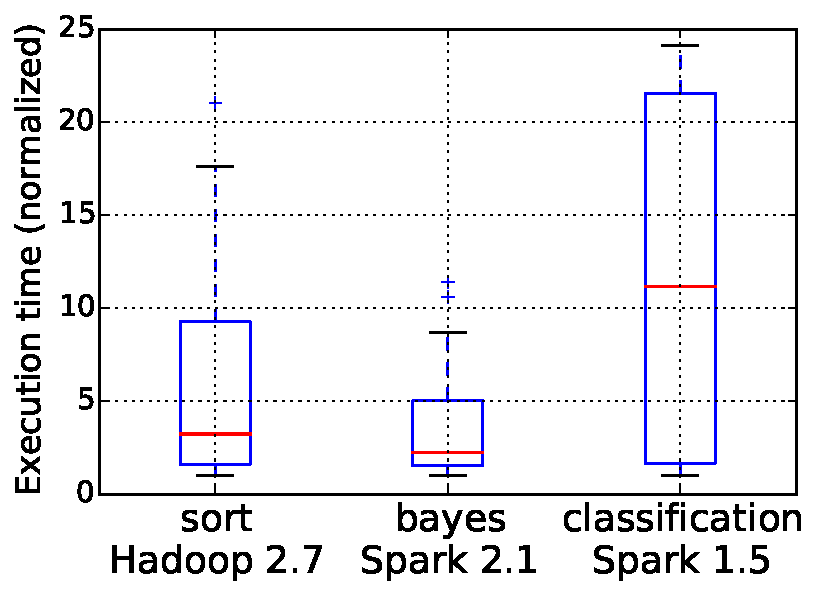
\includegraphics[width=\linewidth]{figures/motivation_bad_choice_time.pdf}
    \caption{Execution time}
    \label{fig:motivation_bad_choice_time}
\end{subfigure}
\hfill
\begin{subfigure}[b]{0.45\textwidth}
    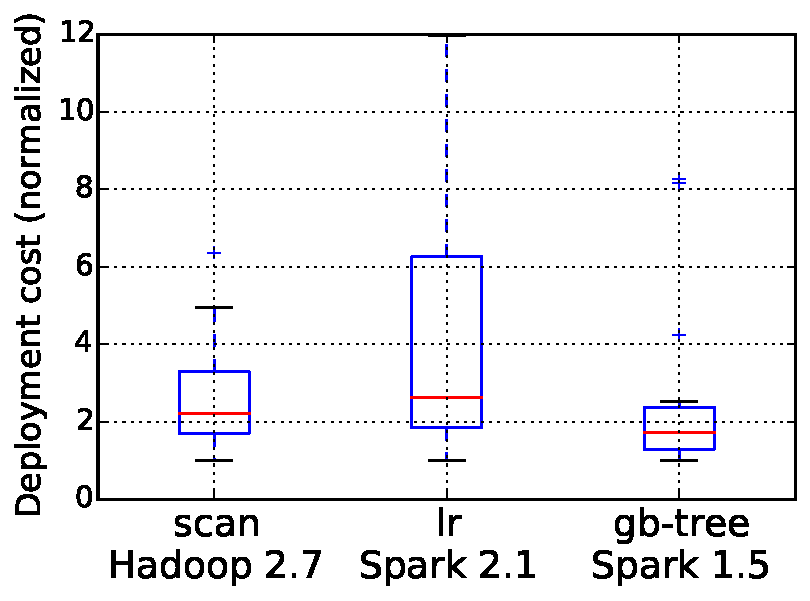
\includegraphics[width=\linewidth]{figures/motivation_bad_choice_cost.pdf}
    \caption{Deployment cost}
    \label{fig:motivation_bad_choice_cost}
\end{subfigure}
\caption{The execution time and deployment cost of workloads running on 18 virtual machines (different types). The execution time of classification-Spark 1.5 in the worst case is 20 times slower that the best VM type. Similarly the deployment cost of running Linear Regression on the worst VM type is 10 times more expensive than the best VM type.}
\label{fig:motivation_bad_choice}
\end{figure}



\subsection*{No VM rules all}
Our empirical data, as shown in \myfigure{\ref{fig:motivation_bad_choice}}, demonstrates that
a bad choice can increase the execution time (of a workload) up to 20 times and can be ten times more costly than the optimal one.
Prior work reports similar results~\cite{Alipourfard2017, Yadwadkar2017}. Careless selection can often end up
with high deployment cost and longer (sub-optimal) execution time.

Even though users are willing to pay a higher cost in exchange for performance, choosing the most expensive VM type may not always result in optimal performance. Figure~\ref{fig:motivation_variance_time} shows the distribution of the execution time when running on the most expensive VM types  (namely c4.2xlarge, m4.2xlarge and r4.2xlarge). For instance, if we look at the distribution of execution times for c4.2xlarge, we observe that c4.2xlarge is the best VM for 50\% of the cases. This means for the other 50\% of the workloads; the most expensive VM type does not guarantee the lowest execution time. We observe similar behavior in Figure~\ref{fig:motivation_variance_cost}, where the least expensive VM, c4.large, does not ensure the lowest deployment cost.

% \myfigure{\ref{fig:motivation_variance_time}} suggests that
% the most expensive VM type can sometimes lead to a ten times slowdown. Possible explanations could be 
% resource bottleneck or resource availability~\cite{Yadwadkar2017}.

% Similarly, when optimizing for cost,
% choosing the cheapest VM type can lead to a higher deployment cost in several cases. \myfigure{\ref{fig:motivation_variance_cost}} shows that the cheapest VM type can increase the deployment cost up to more than eight times.
% Hence, there does not exist an one-size-fits-all VM type.


\begin{figure}
\centering
\begin{subfigure}[b]{0.45\textwidth}
    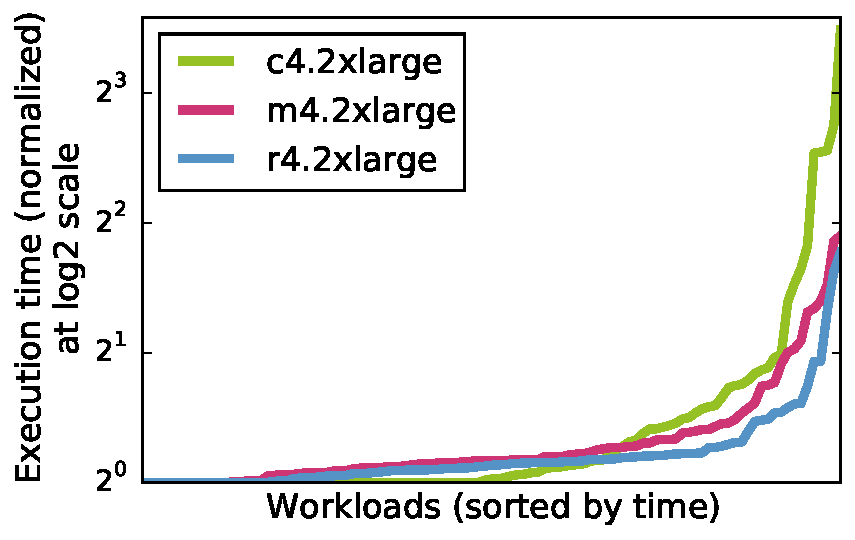
\includegraphics[width=\linewidth]{figures/motivation_variance_time.pdf}
    \caption{Execution time on the most expensive VM types.}
    \label{fig:motivation_variance_time}
\end{subfigure}
\hfill
\begin{subfigure}[b]{0.45\textwidth}
    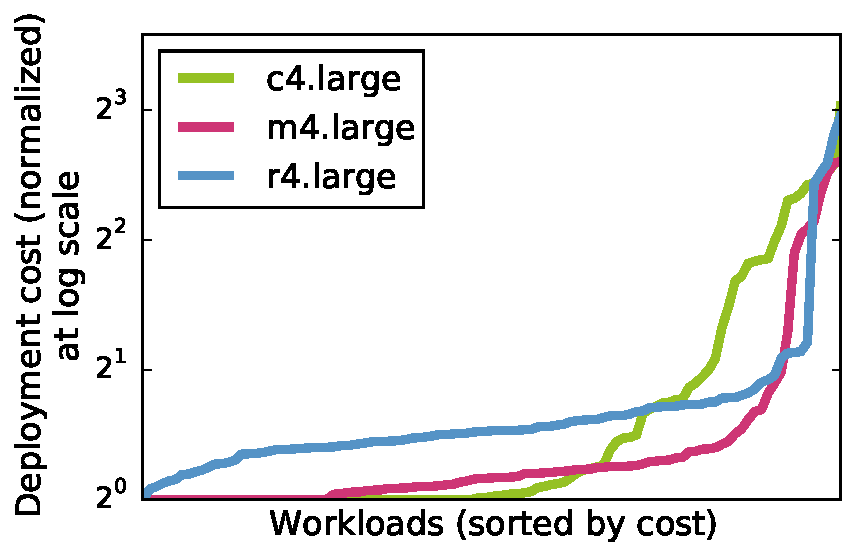
\includegraphics[width=\linewidth]{figures/motivation_variance_cost.pdf}
    \caption{Deployment cost on the least expensive VM types.}
    \label{fig:motivation_variance_cost}
\end{subfigure}
\caption{Performance distribution over different workloads. The performance is normalized to the optimal performance measured in the 18 virtual machines. The \emph{x-axis} represents workloads, sorted by their normalized performance.  Both choosing the most expensive and the cheapest VM types are not desirable.}
\label{fig:motivation_variance}
\end{figure}





\subsection*{The same application with different input sizes favors different VM types}
Machine learning workloads are readily available
such as the machine learning library in Apache Spark and Python~\cite{scikit-learn}.
It is valid to assume that similar workloads would prefer the same VM type provided the user can accurately identify similar workloads.
Consequently, users can always reuse the best VM type for their workloads without testing further.
However, we found that this might not always be the case.
A workload with different input sizes or parameters performs very differently on different VMs~\cite{Venkataraman2016}.
Figure~\ref{fig:motivation_datasize} illustrates how the performance of an application varies with different input sizes.
For example, in Figure~\ref{fig:motivation_datasize_b}
\emph{c4.large} is the most cost-effective VM type for running the \textit{bayes} application with the \emph{small} input size.
However, the deployment cost increases by 40\% (is no longer the optimal VM) when the input size is \emph{large}.
A possible explanation is that a larger input size creates
a resource bottleneck on a smaller VM.
Hence, users need to be more careful
at selecting the best VM type even for the same applications.



\begin{figure}
\centering
\begin{subfigure}[b]{0.45\textwidth}
    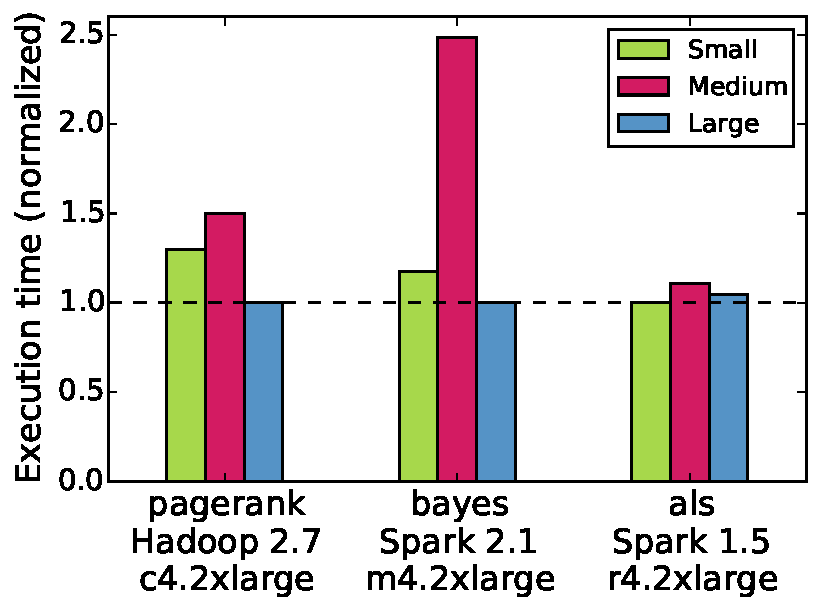
\includegraphics[width=\linewidth]{figures/motivation_datasize_time.pdf}
    \caption{Execution time.}
    \label{fig:motivation_datasize_a}
\end{subfigure}
\hfill
\begin{subfigure}[b]{0.45\textwidth}
    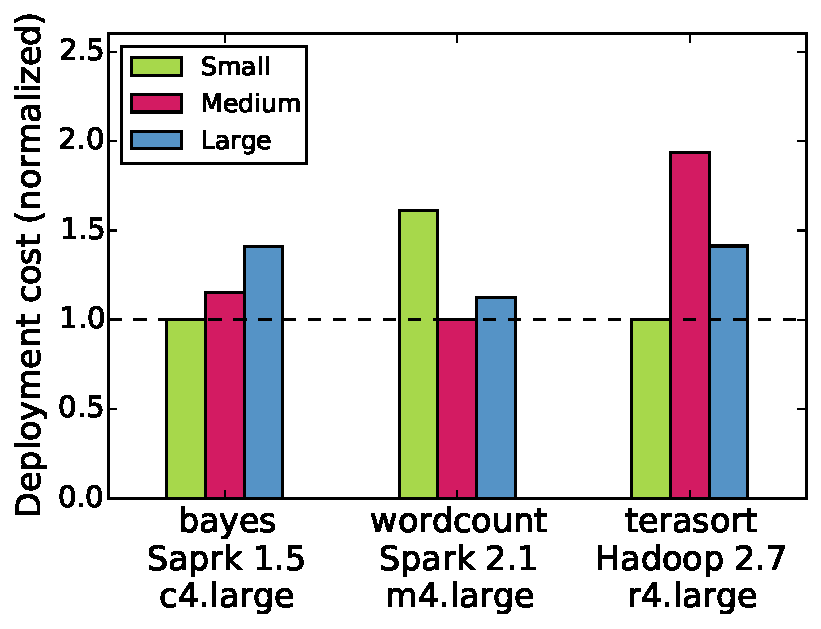
\includegraphics[width=\linewidth]{figures/motivation_datasize_cost.pdf}
    \caption{Deployment cost.}
    \label{fig:motivation_datasize_b}
\end{subfigure}
\caption{Running application with different input sizes result in very different performance.
 The best performing VM types for an application can change when the input size or parameters are changed.}
\label{fig:motivation_datasize}
\end{figure}



\subsection*{Cost creates a level playing field}
Finding a cost-effective VM type can be harder because
a slower VM can be competitive in deployment cost.
In \myfigure{\ref{fig:motivation_variance_time}},  \emph{c4.2xlarge} is the fastest VM type for over 50\% of the workloads (optimal execution time is 1.0).
However in Figure~\ref{fig:motivation_variance_cost}, when considering deployment cost, we observe that
\emph{c4.large} is likely to be a better choice, since it is optimal VM in over 50\% of the workloads.

\myfigure{\ref{fig:level_playing_field}} presents the normalized execution time
and deployment cost of a workload (\emph{regression} on \emph{Spark 1.5}).
The figure demonstrates how execution time can be very different
while deployment cost is similar across all VM types. For example, \emph{m4.large} and \emph{c4.xlarge} are comparable to \emph{c4.2xlarge} in terms of deployment cost.
When the difference between execution times of a workload in different VM types is large, choosing the best VM is easier because there is a clear winner.
Incorporating cost compresses the difference.
Therefore, searching for the most cost-effective VM type becomes more difficult because several inferior choices (in terms of execution time) are now competitive (in deployment cost).
In Section~\ref{sec:comparison}, we show why finding cost-effective VM type
is harder than execution time.


\begin{figure}
    \centering
    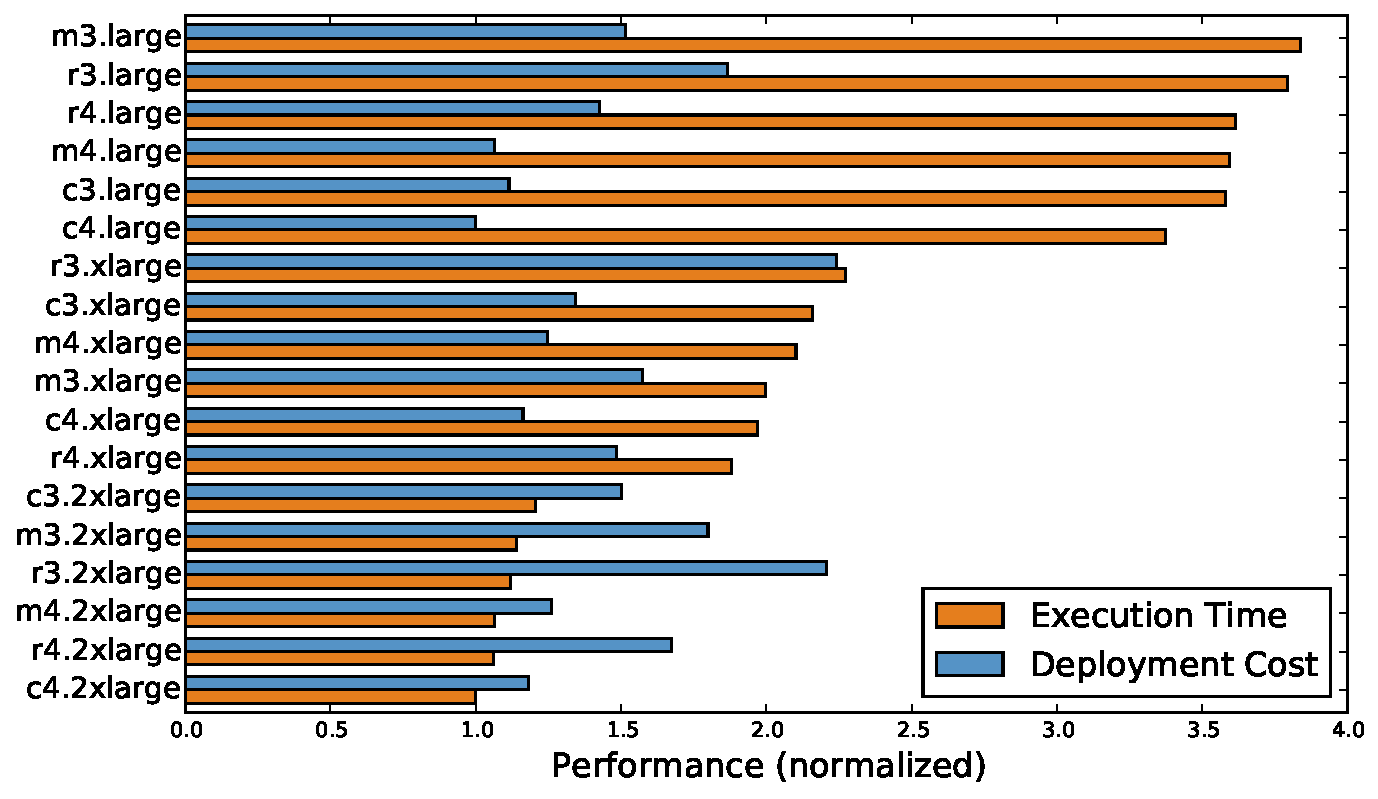
\includegraphics[width=0.8\textwidth]{figures/level_playing_field.pdf}
    \caption{The performance of running the \emph{regression} workload on instances with different VM types.
    Introducing cost creates a \emph{level playing filed}, in which several inferior VM types in execution time are now competitive in deployment cost.
    This observation implies that searching for the most cost-effective configuration is harder than searching for the fastest configuration.}
    \label{fig:level_playing_field}
\end{figure}
\section{State-of-the-Art Approaches}
\label{sec:cat::relatedwork}

\iffalse
Cloud providers recommend the choice of VM types~\cite{aws, google_rightsizing}.
However, it is too coarse grain and does not
apply to many workloads because
resource requirement is often opaque~\cite{Yadwadkar2017}.
This paper address the CAT problem, which is non-trivial
for the following reasons
~\cite{Venkataraman2016,Alipourfard2017,Yadwadkar2017,Hsu2018Arrow}.

\begin{itemize}
\item \textbf{Brute Force.}There are more than 100 cloud configurations.
Consequently, evaluating all the possible configurations
to find the best configuration is too expensive.

\item \textbf{Canonical Cloud Configuration.}
Each workload---application and input---has its own preferred choice
of cloud configuration.
Therefore, there is no one-size-fits-all configuration
~\cite{Alipourfard2017,Hsu2018Arrow,Venkataraman2016}. 

\item \textbf{Opaque Resource Requirements.}
Resource requirements to achieve a certain objective
(execution time or running cost)
for a specific workload are opaque~\cite{Yadwadkar2017}.

\item \textbf{Level playing field.}
While the execution time tends to decrease with a more powerful instance type,
the cost per unit time goes up, which compresses the running costs.
This creates a level playing field---several inferior configurations
in execution time are now competitive in running cost~\cite{Hsu2018Arrow}.
Consequently, it is harder to find the optimal cloud configuration
when the performance goal is reducing cost.

\end{itemize}

\fi



The CAT problem can be cast into 
a \emph{learning problem}---which uses elaborate offline evaluation
to generate a machine learning model that predicts the performance of workloads
~\cite{Venkataraman2016, Yadwadkar2017}
and an \emph{optimization problem}---which successively evaluates configurations
looking for one that is near optimal~\cite{Alipourfard2017, Hsu2018Arrow}.

Prediction, as proposed in PARIS~\cite{Yadwadkar2017},
is not reliable because of high variance in prediction results. 
Prediction accuracy heavily relies on feature selection, model selection,
and parameter tuning and the quality of data.
Sequential Model-Based Optimization (SMBO)~\cite{Dewancker2015}
is a search-based optimization method, which
does not require an accurate model but can have
a high evaluation cost (measured in terms of configurations evaluated).
Bayesian Optimization (used in \emph{CherryPick}) falls into
the SMBO class of algorithms.

The state of the art techniques such as
CherryPick~\cite{Alipourfard2017} and PARIS~\cite{Yadwadkar2017}
suffer from three major issues. 

\begin{itemize}
\item \textbf{Model accuracy.}
Prediction based approaches like PARIS build a model using measurements. The objective of such an approach is to use an accurate model to predict,
for example, execution time or running cost of workloads.
This method has two major weaknesses (i) building an accurate model requires more data---which in our setting is hard to come by, and (ii) the performance of the cloud environment is susceptible to performance variability---the data collected after running the workload might not reflect the true performance~\cite{tang2011impact}.
As shown in PARIS, the performance of batch-processing jobs is less predictable.
The inaccurate estimation of the execution time can be attributed to the non-linear relationship between resource and performance~\cite{Alipourfard2017}. 

\item \textbf{Cold-start}
Any SMBO method requires initial measurements to seed the search process.
The initial measurements are very crucial since
it determines the effectiveness of the search.
A poor seeding strategy can lead to wasted effort and
can yield a sub-optimal cloud configuration.
The effect of cold-start is more pronounced when 
the initial measurement cost cannot be amortized,
\eg{the search space is not large enough.}

\item \textbf{Fragility}
An SMBO method is fragile as it is overly sensitive to input parameters.
The success of \emph{CherryPick} on a given workload depends on the initial points used to seed the search and the choice of the kernel function used in the performance model (Gaussian Process Model).
Previous work shows that \emph{CherryPick}
sometimes fails to find near-optimal configurations and
incurs longer (than expected) search path~\cite{Hsu2018Arrow}.

\end{itemize}


Hyper-parameter tuning shares similarity with CAT.
For example, system and software performance is highly affected by configurations.
StarFish is an auto-tuning system for Hadoop applications~\cite{herodotou2011starfish}.
\emph{BestConfig} proposes the Divide and Diverge Sampling strategy along with the Recursive Bound and Search method
for turning software parameters~\cite{zhu2017bestconfig}.
A similar framework is also proposed to automate tuning system performance
of stream-processing systems~\cite{bilal2017towards}.
BOAT is a structured Bayesian Optimization-based framework for automatically tuning system performance
~\cite{Dalibard2017} which leverages contextual information.
Sampling techniques focus on reducing sampling cost while building accurate models to optimize software systems \cite{oh2017finding, nair2017}.
Parameter tuning is also an critical in machine learning~\cite{Dewancker2015,shahriari2016taking,Klein2017,golovin2017google}. 

The above methods focus on performance tuning for the same workload (or application)
on the same type of architecture.
It is still not clear how to leverage their approaches
to support different architectural configurations in cloud computing.



\section{Problem Formalization}

Cloud architecture tuning (CAT) finds the best cloud configuration
for a workload ($w\in W$)---an application and its input.
\emph{IaaS} provides a set of computation, storage, and network resources.
For example, users have to determine the type and the number of VMs
to run a workload.
The search space ($S$) is a valid set of
architectural configurations for running the given workload.
The size of the search space is $|S|$ configurations
(the search space is the same for all workloads).
For a given workload $w$,
each configuration $s \in S$ has a corresponding cost measure $y=\phi(w, s)$.
The objective function, $\phi$, is user-specific.
In practice, cost measures can include
execution time, query throughput, running cost, etc. 

A cloud service provider presents its user with several choices of VM types ($\mathit{VM}$).
Let $\mathit{VM}_i$ indicate the $i^{th}$ VM type in the list of VMs.
%, which takes a value from a finite domain $Dom(\mathit{VM}_i)$.
In general, each VM type has distinct characteristics (such as memory size and core counts).
%$\mathit{VM}_i$ indicates the published characteristics of VMs (such as memory size and core counts).
%$\mathit{VM}_{ij}$ represents the $j^{th}$ characteristic of the $i^{th}$ VM type. The \textit{instance space} is thus $Dom(\mathit{VM}_1) \times Dom(\mathit{VM}_2) \times ... \times Dom(\mathit{VM}_n)$, which is the Cartesian product of the domains, where $n = \left\vert{\mathit{VM}}\right\vert$ is the number of VMs provided by the cloud service provider. 
When a workload ($w\in W$) is run on a VM ($\mathit{VM}_i$), the low-level metrics ($l_{i,w}\in L$) can be collected from the VM.
%These low-level metrics are denoted by $l_i$.
Each VM type ($\mathit{VM}$) has a corresponding performance measure $y\in Y$ (\eg{time or cost}).
We denote the performance measure associated with a given VM type and a workload by $y_{i,w}=f(\mathit{VM}_{i,w})$.
In this setting, $\mathit{VM}_{i,w}$ and $y_{i,w}$ are the independent and dependent variables, respectively.

An effective CAT method must
find (near) optimal configurations and
exhibit low \emph{search cost}.

\subsection*{Search performance}
Let $y^{*}$ be the optimum (minimum) cost for a workload, 
\emph{i.e.},
$y^* = \min_{\forall s \in S} \phi(w, s)$.
Let $\hat{y}$ be the best workload performance that a CAT optimizer finds.
The search performance of the CAT optimizer is $\hat{y}/y^{*}$
(lower the better).
A brute force approach finds the optimal configuration for a given workload.
Existing methods such as \emph{CherryPick} and \emph{Arrow} achieve
near-optimal search performance (\eg{$<1.1$}).

\subsection*{Search cost}
A CAT optimizer must evaluate a workload
on several architectural configurations to determine the best choice.
Such evaluation is generally expensive.
\emph{CherryPick} needs to evaluate at least three configurations
when running Bayesian Optimization and
\emph{PARIS} generates the fingerprint using two evaluations.
Let $E \subset S$ represent the search space that a CAT optimizer evaluated.
We define search cost as $|E|$---the number of evaluations needed to
select a configuration.
This measure is intuitive and effective to compare different CAT methods.
Other possible measures are
evaluation cost (dollars) and evaluation duration (time).

Our goal is to design a search method to:
\begin{enumerate}[leftmargin=*]
    \item \textit{Minimize} the performance difference between
the \emph{best} VM  ($\mathit{VM^*}$) (found by search) and the optimal VM  ($\mathit{VM}^{opt})$. We find $\mathit{VM^*}$ both in terms of \textit{execution time} and \textit{deployment cost};
    \item \textit{Minimize} search cost---the number of measurements required to find the (near) optimal configuration.
\end{enumerate}

We also look at other metrics for comparing CAT methods.
First, it is important to deliver \emph{reliable}
search performance and search cost across different workloads.
Some optimizers may encounter the fragility issue because
the search space is hard to model~\cite{Hsu2018Arrow}.
Second, a CAT method must be \emph{scalable}.
\emph{Ernest}, for example, must build a prediction model
for each VM family. 
Last, the optimizer must use a generic approach for adapting to
the rapid changes in cloud computing and software systems.
Exploiting workload information and system internals
can improve prediction performance but
makes a CAT method less applicable to distinct systems
~\cite{Wang2004,Venkataraman2016}.

\section{Time-Cost Trade-Offs}
\label{sec:cdp}



When hosting applications in the cloud,
users can choose the \emph{fastest} configuration regardless of cost
or the \emph{cheapest} configuration without the time constraint.
Neither choice is truly piratical.
There is always a trade-off between \emph{time} and \emph{cost}.
Users are willing to spend more on resources when
time is more critical (hard deadline) or
the increase in cost expects reasonable decrease in execution time (soft deadline).
Similarly, when the time constraint is relaxed, users accept
slower configuration but with higher cost saving.

We propose using cost-delay product (CDP),
similar to energy-delay product (EDP)~\cite{Freeh2007},
to analyze the trade-offs
for choosing the cloud configurations of data-intensive applications.
CDP puts the same importance on time and cost.
For example,
a $5\%$ slow down in execution time
is enough to justify
a $5\%$ cost saving.
$CD^2P$ and $C^2DP$, on the other hand, shift the importance to
time and cost respectively.
When the time improvement is $1\%$ but it incurs $50\%$ increase in cost,
users will probably choose the slower configuration.


We run three real-world applications,
\emph{PageRank},
\emph{web log analysis}, and
\emph{regression},
on Apache Spark, a distributed, large-scale data processing system \cite{spark}.
We conduct a series of evaluations of the three applications against
different resource costs by varying
the number of CPUs (from 1 to 12)
and
the size of memory (from 1 to 4 GB per CPU).
We measure the execution time to complete the applications.
\mytable{\ref{table:raw_data}} lists their time and cost in detail.
\myfigure{\ref{fig:application_performance}} uses a scatter plot
to show 
the execution time of applications running against different resource \emph{costs}.
We find that their distribution patterns are not totally alike.
Therefore, there does not exist one best configuration for all applications.
Even within the same applications, execution time can change dramatically.
\myfigure{\ref{fig:application_performance}} also illustrates a convex hull
for outcomes bounded to a subset of the plane.
When choosing the \emph{best} configuration, the solution must be close to the
convex hull.

\begin{table}[!htbp]
\centering
\caption{The execution time and resource cost of applications
running with different numbers of CPUs and memory per CPU.
The text in bold refer to the configurations on the convex hull
in \myfigure{\ref{fig:application_performance}}.}
\label{table:raw_data}
\begin{tabular}{rrrrrrrrr}
\multicolumn{3}{c}{\textbf{Configuration}}  & \multicolumn{2}{c}{\textbf{PageRank}} & \multicolumn{2}{c}{\textbf{Web Log Analysis}} & \multicolumn{2}{c}{\textbf{Regression}}\\
ID  & CPU & Memory/CPU & Time & Cost & Time & Cost & Time & Cost \\ \hline \hline
0   & 1          & 1       & 652.2 & 3261.1  & \textbf{179.3} & \textbf{896.3}  & \textbf{765.0}  & \textbf{3825.2} \\
1   & 1          & 2       & 389.2 & 2335.3  & 220.2 & 1321.1 & 706.7  & 4240.1 \\
2   & 1          & 4       & 267.7 & 2141.8  & 187.8 & 1502.4 & 723.7  & 5789.7 \\
3   & 1          & 8       & 240.3 & 2883.6  & 210.1 & 2521.1 & 701.0  & 8412.0 \\ \hline
4   & 2          & 1       & 234.6 & 2346.3  & \textbf{99.5}  & \textbf{994.6}  & \textbf{423.4}  & \textbf{4233.6} \\
5   & 2          & 2       & \textbf{139.1} & \textbf{1669.1}  & 104.3 & 1252.0 & 433.3  & 5200.1 \\
6   & 2          & 4       & 151.3 & 2420.0  & 123.8 & 1980.1 & 407.8  & 6524.6 \\
7   & 2          & 8       & 152.4 & 3657.0  & 121.6 & 2919.5 & 434.0  & 10414.2 \\ \hline
8   & 4          & 1       & \textbf{93.2}  & \textbf{1864.5}  & \textbf{63.0}  & \textbf{1259.5} & \textbf{269.1}  & \textbf{5382.2} \\
9   & 4          & 2       & 96.2  & 2310.0  & 74.2  & 1781.1 & \textbf{261.7}  & \textbf{6280.3} \\
10  & 4          & 4       & 95.7  & 3063.2  & 71.0  & 2270.8 & 268.7  & 8598.7 \\
11  & 4          & 8       & 101.0 & 4846.5  & 68.0  & 3262.1 & 275.9  & 13242.1 \\ \hline
12  & 8          & 1       & \textbf{70.3}  & \textbf{2811.5}  & \textbf{47.3}  & \textbf{1892.5} & 817.8  & 32711.8 \\
13  & 8          & 2       & 72.4  & 3475.4  & 47.5  & 2277.8 & 842.3  & 40431.1 \\
14  & 8          & 4       & 75.4  & 4828.5  & 55.0  & 3515.8 & 711.2  & 45518.7 \\
15  & 8          & 8       & 70.7  & 6783.4  & 46.8  & 4488.7 & 692.7  & 66502.3 \\ \hline
16  & 12         & 1       & 71.2  & 4272.9  & 48.1  & 2887.0 & 983.5  & 59007.1 \\
17  & 12         & 2       & \textbf{69.6}  & \textbf{5007.7}  & \textbf{46.0}  & \textbf{3309.2} & 1043.4 & 75122.3 \\
18  & 12         & 4       & 72.0  & 6912.8  & \textbf{45.4}  & \textbf{4357.1} & 1026.6 & 98549.5 \\
19  & 12         & 8       & 73.7  & 10617.9 & 49.9  & 7180.6 & 940.0  & 135362.0
\end{tabular}
\end{table}



In the PageRank case, for example,
users are more likely to choose four CPUs instead of eight CPUs because
25\% reduction in execution time requires
more than 50\% extra cost.
We explain the three applications' trade-off as follows.

\subparagraph*{PageRank}

PageRank is an ranking algorithm to calculate the importance of website pages
by counting the number of links to them.
Our evaluation has shown that execution time decreases as
we increase the number of CPUs.
Although \emph{PageRank} exhibits shorter execution time
when the CPU count is greater than eight,
it more makes sense to choose four CPUs as it is more cost effective,
as depicted in~\myfigure{\ref{fig:pagerank_cost}}.
However, when time is more critical ($CD^2P$),
~\myfigure{\ref{fig:pagerank_time}} shows that
eight CPUs is a better choice.

\subparagraph*{Web Log Analysis}
This application tracks the query counts and aggregate bytes in a particular group.
The CPU count greatly affects the execution time but memory size does not
show significant impact.
As shown in~\myfigure{\ref{fig:webloganalysis_time}}, a larger number of CPUs (increasing from 1 to 4)
increase resource costs but time reduction is large enough
to compensate the increase in cost.
This is not the case when the CPU count is more than four.
When time is more critical, $CD^2P$ suggests eight CPUs is a viable configuration.

\subparagraph*{Regression}
The regression application generates a function that estimates 
the relationships among variables.
Different from the above two applications, \emph{regression} shows
more CPU counts do no necessarily help reduce execution time.
It is even worse.
One possible explanation is the overhead by increasing parallelism overcomes
the benefits by higher parallelism.

\begin{figure}
    \captionsetup{justification=centering}
    \centering
    \begin{subfigure}[b]{0.3\textwidth}
        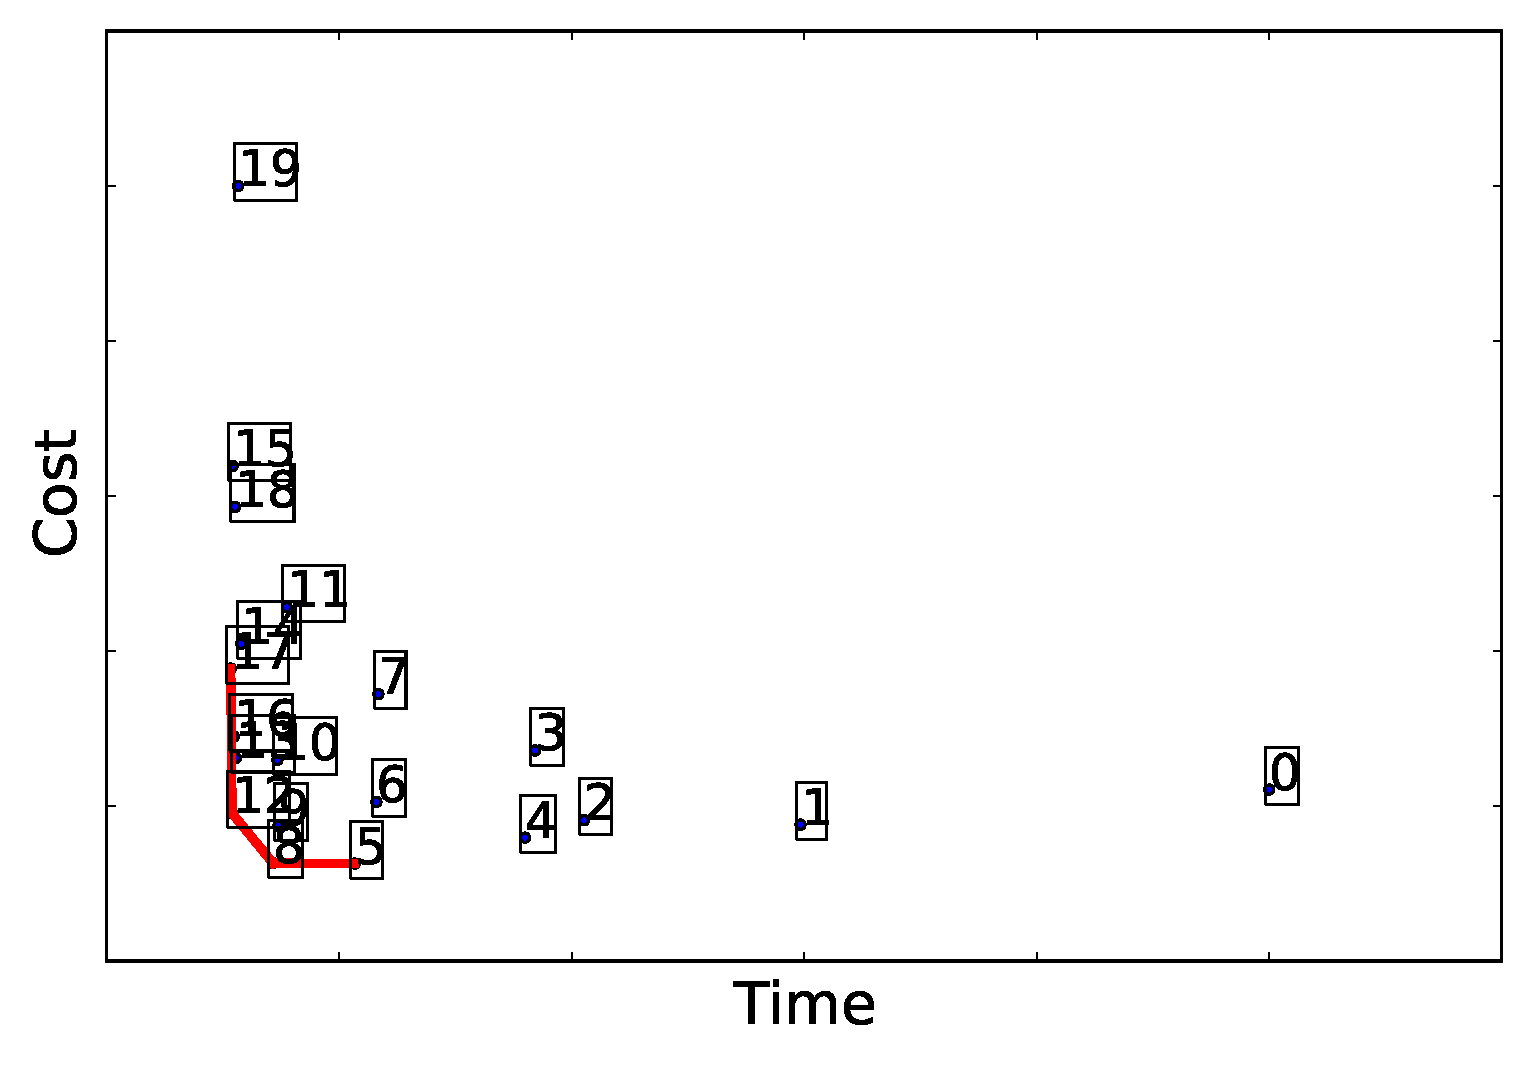
\includegraphics[width=\textwidth]{Chapter-CAT/figures/pagerank_elapsed_cost_all_frontier.eps}
        \caption{PageRank}
        \label{fig:pagerank_configurations}
    \end{subfigure}
    \begin{subfigure}[b]{0.3\textwidth}
        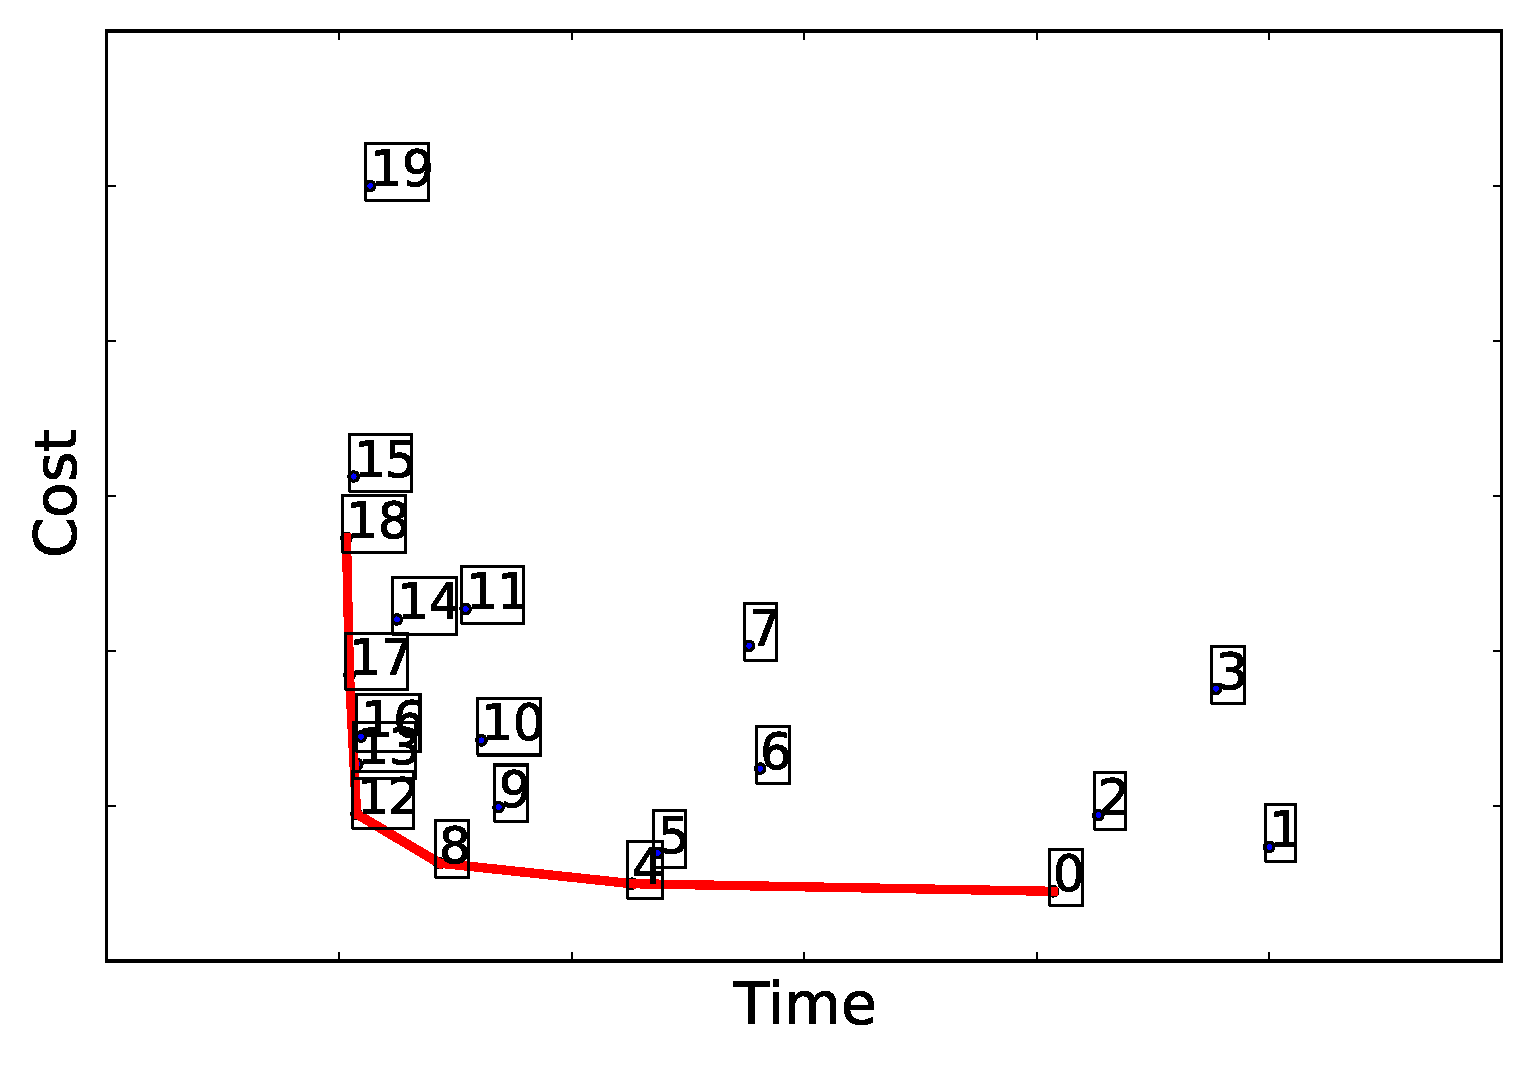
\includegraphics[width=\textwidth]{Chapter-CAT/figures/webloganalysis_elapsed_cost_all_frontier.eps}
        \caption{Web Log Analysis}
        \label{fig:webloganalysis_configurations}
    \end{subfigure}
    \begin{subfigure}[b]{0.3\textwidth}
        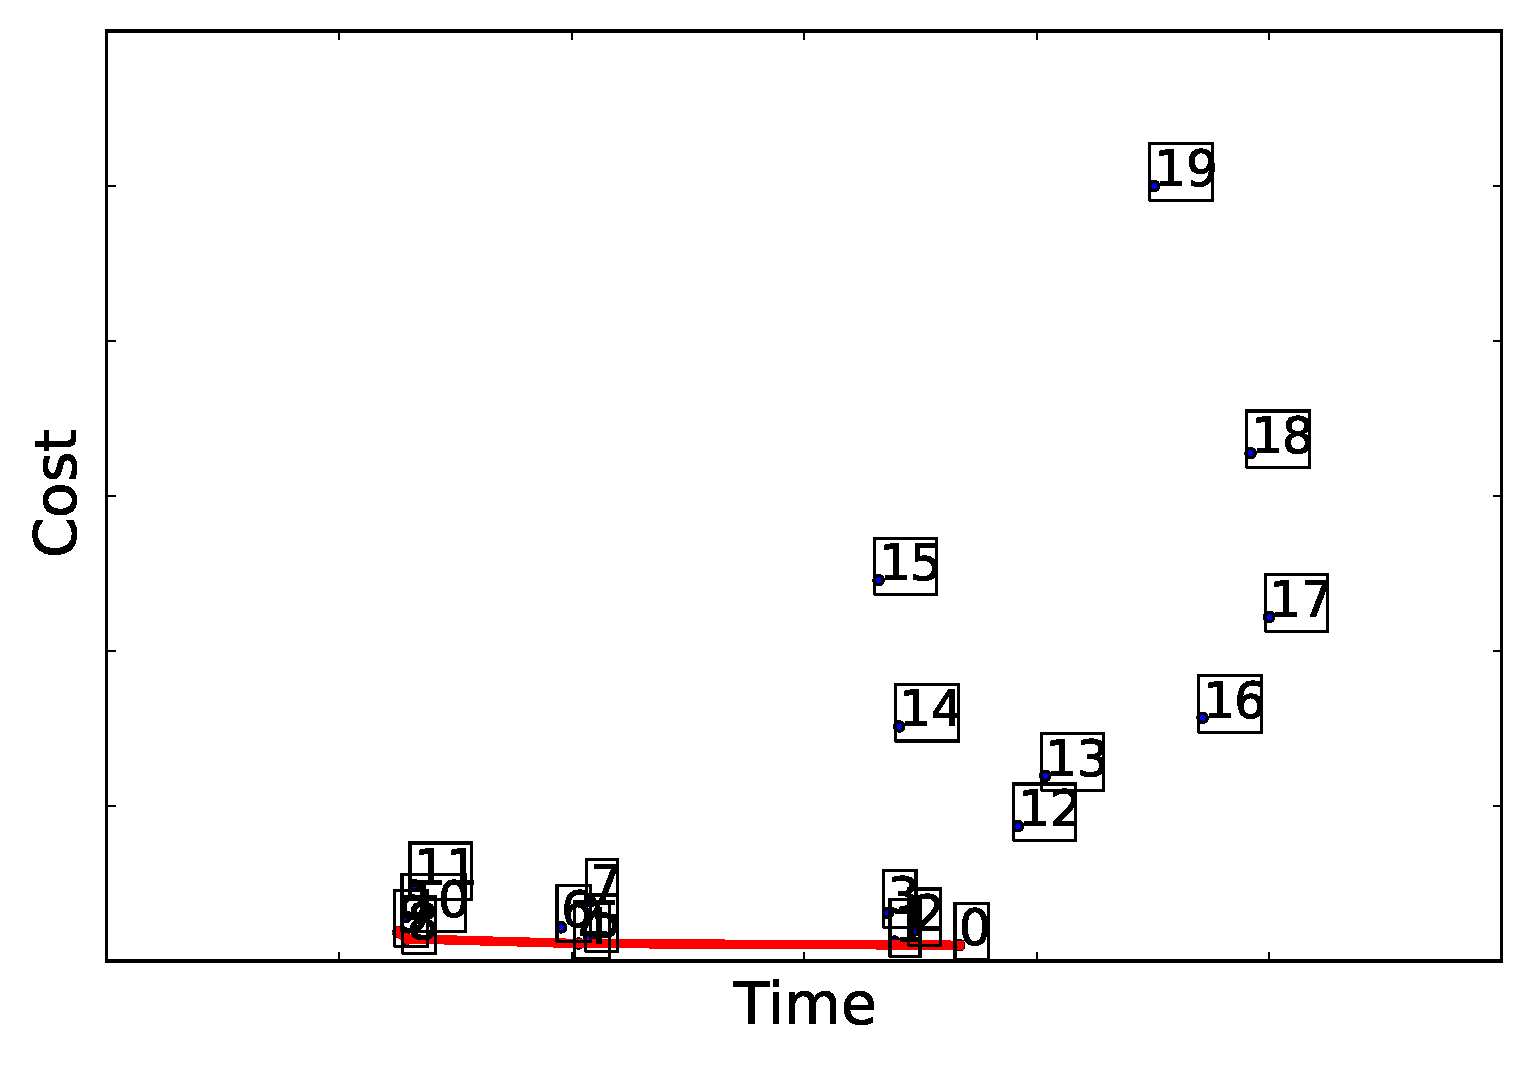
\includegraphics[width=\textwidth]{Chapter-CAT/figures/regression_elapsed_cost_all_frontier.eps}
        \caption{Regression}
        \label{fig:regression_configurations}
    \end{subfigure}
    \caption{Applications' execution time and resource costs with different configurations.}
    \label{fig:application_performance}
\end{figure}


\begin{figure}
    \captionsetup{justification=centering}
    \centering
    \begin{subfigure}[b]{0.3\textwidth}
        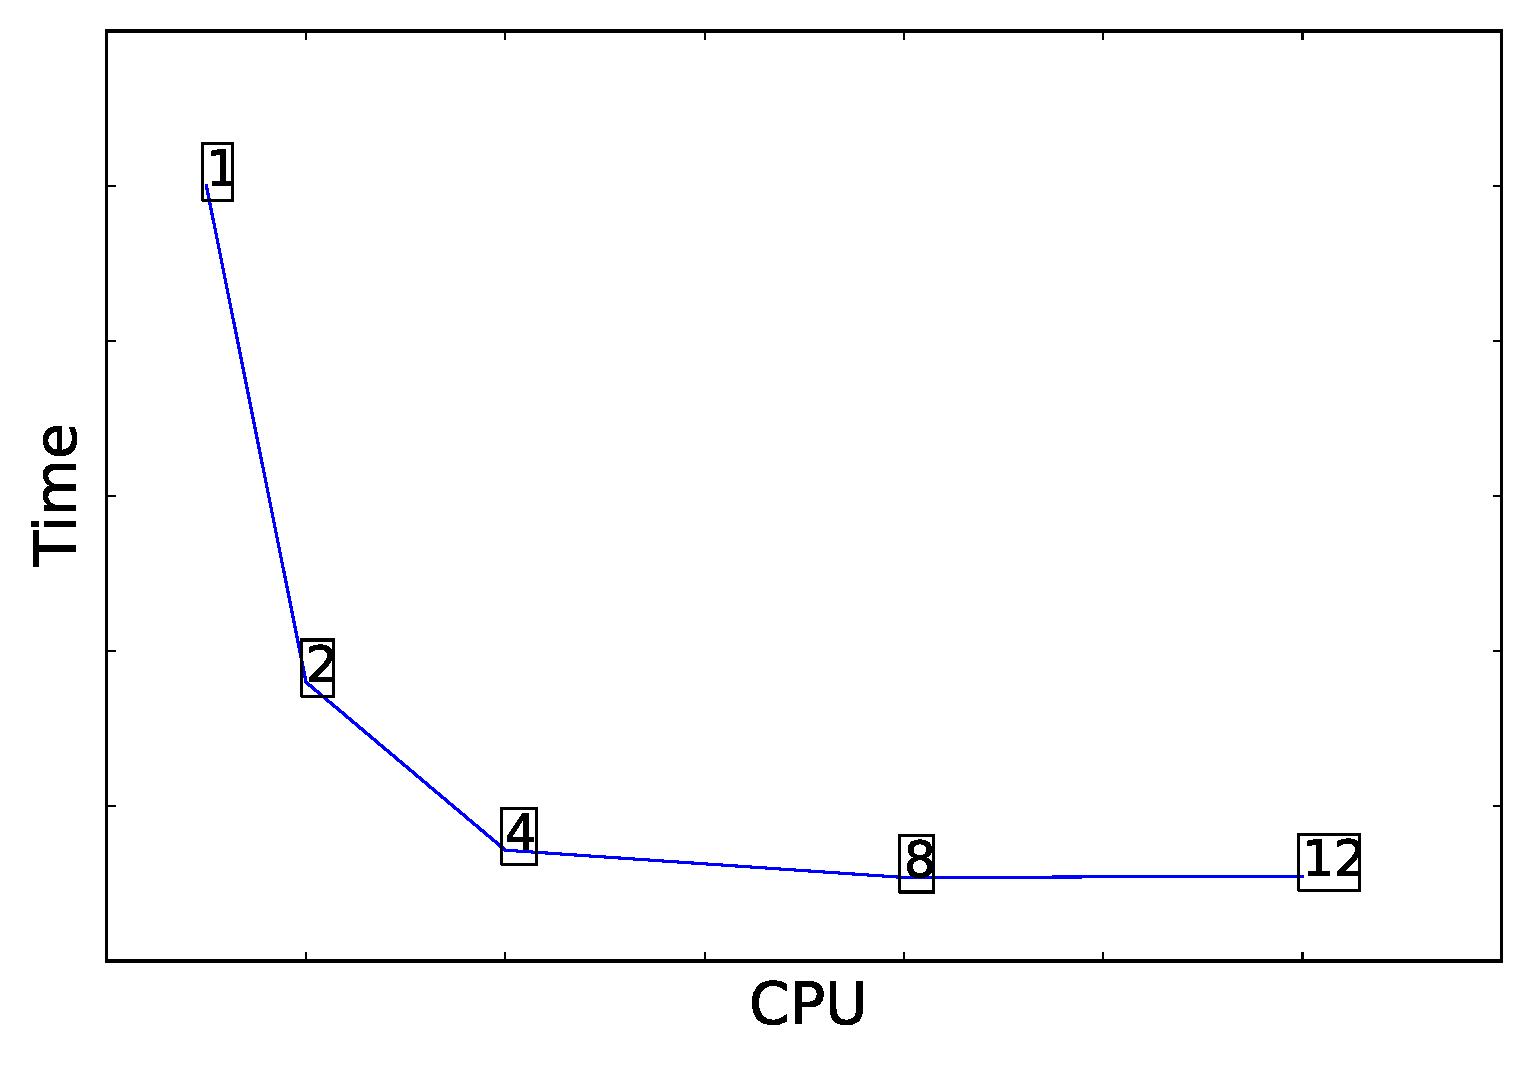
\includegraphics[width=\textwidth]{Chapter-CAT/figures/pagerank_cpu_elapsed_12_1.eps}
        \caption{PageRank}
        \label{fig:pagerank_time}
    \end{subfigure}
    \begin{subfigure}[b]{0.3\textwidth}
        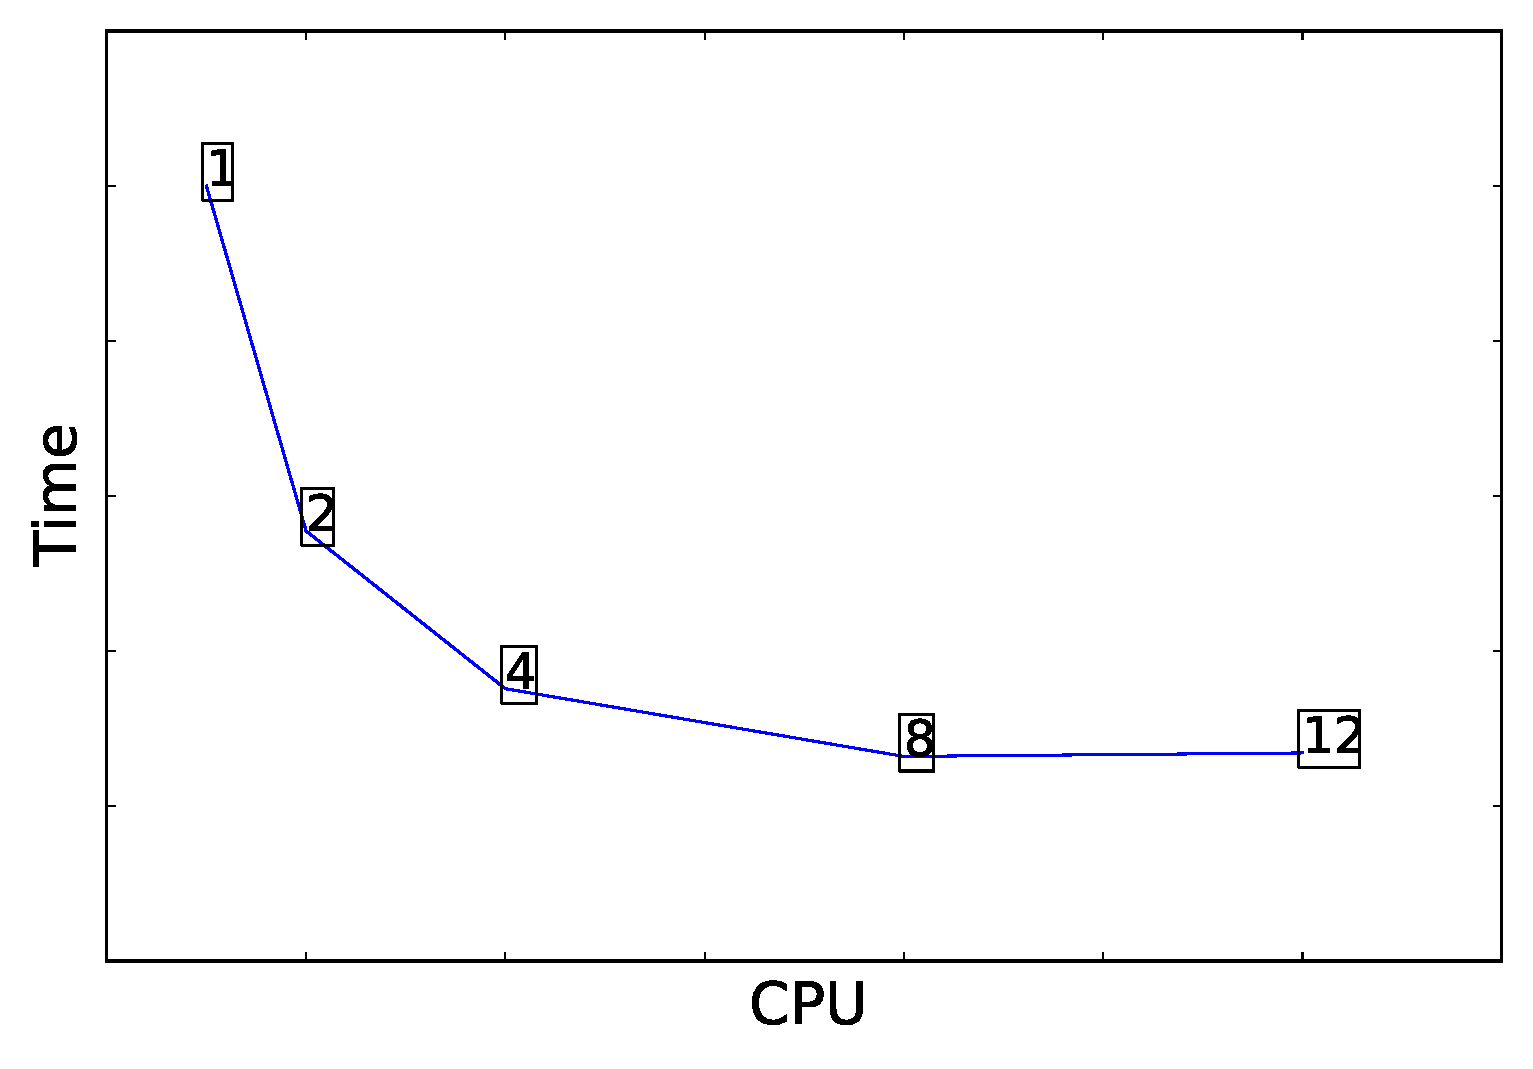
\includegraphics[width=\textwidth]{Chapter-CAT/figures/webloganalysis_cpu_elapsed_12_1.eps}
        \caption{Web Log Analysis}
        \label{fig:webloganalysis_time}
    \end{subfigure}
    \begin{subfigure}[b]{0.3\textwidth}
        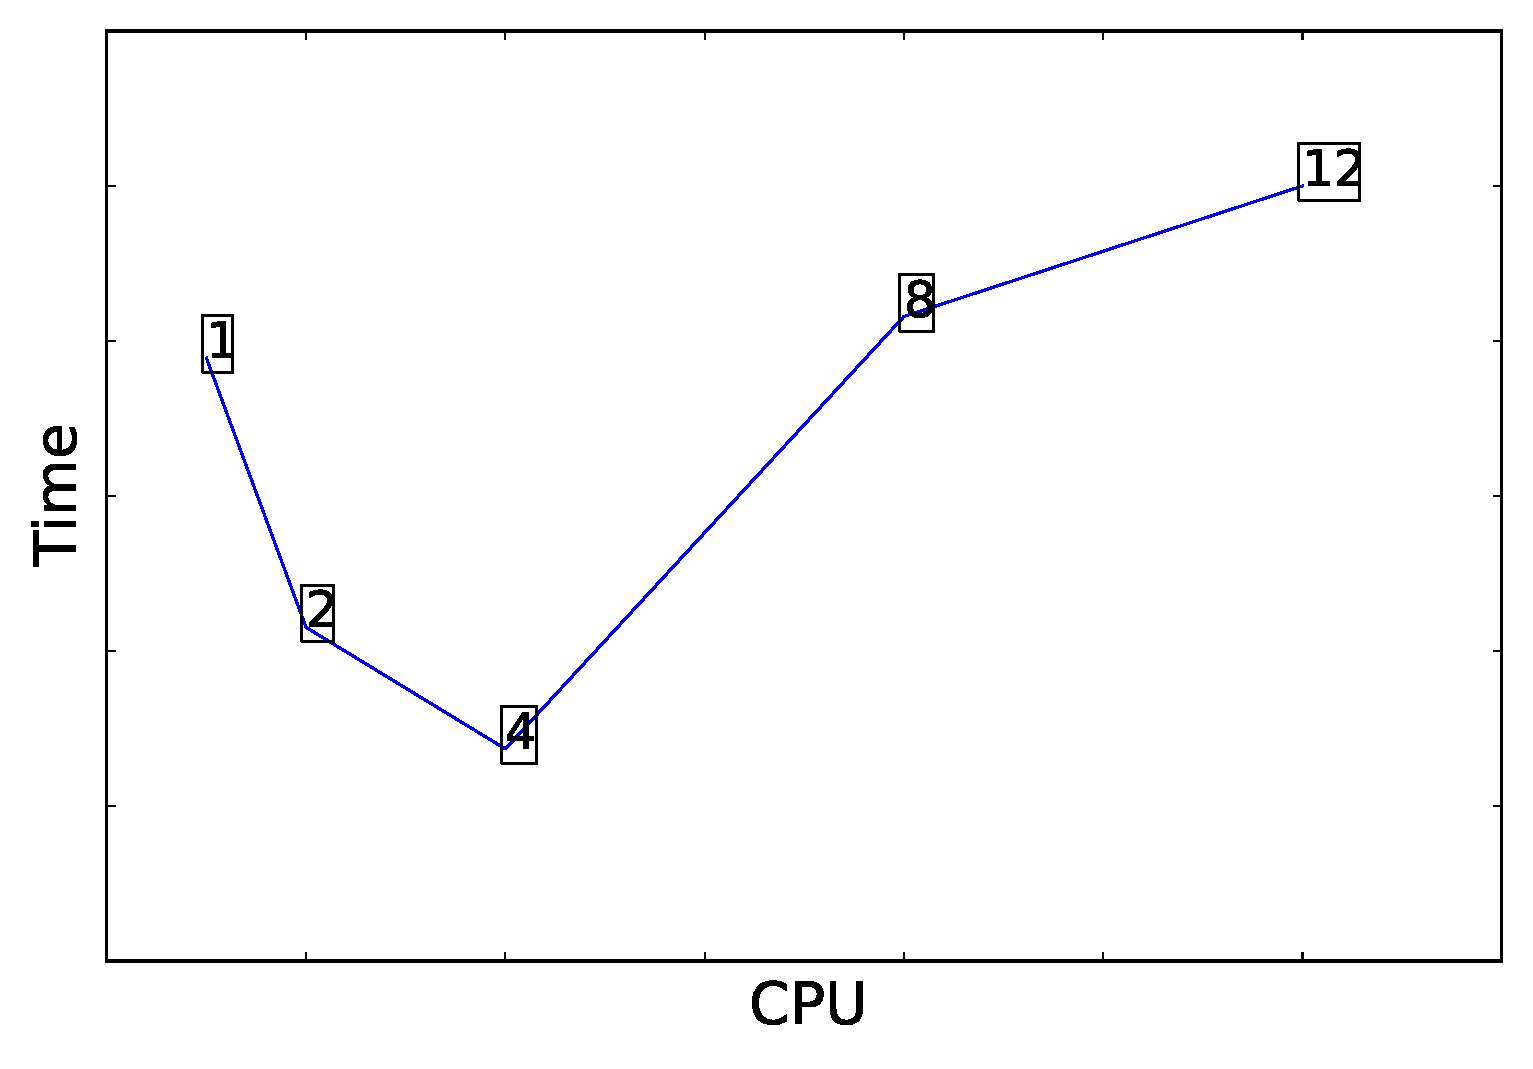
\includegraphics[width=\textwidth]{Chapter-CAT/figures/regression_cpu_elapsed_12_1.eps}
        \caption{Regression}
        \label{fig:regression_time}
    \end{subfigure}
    \bigskip
    \begin{subfigure}[b]{0.3\textwidth}
        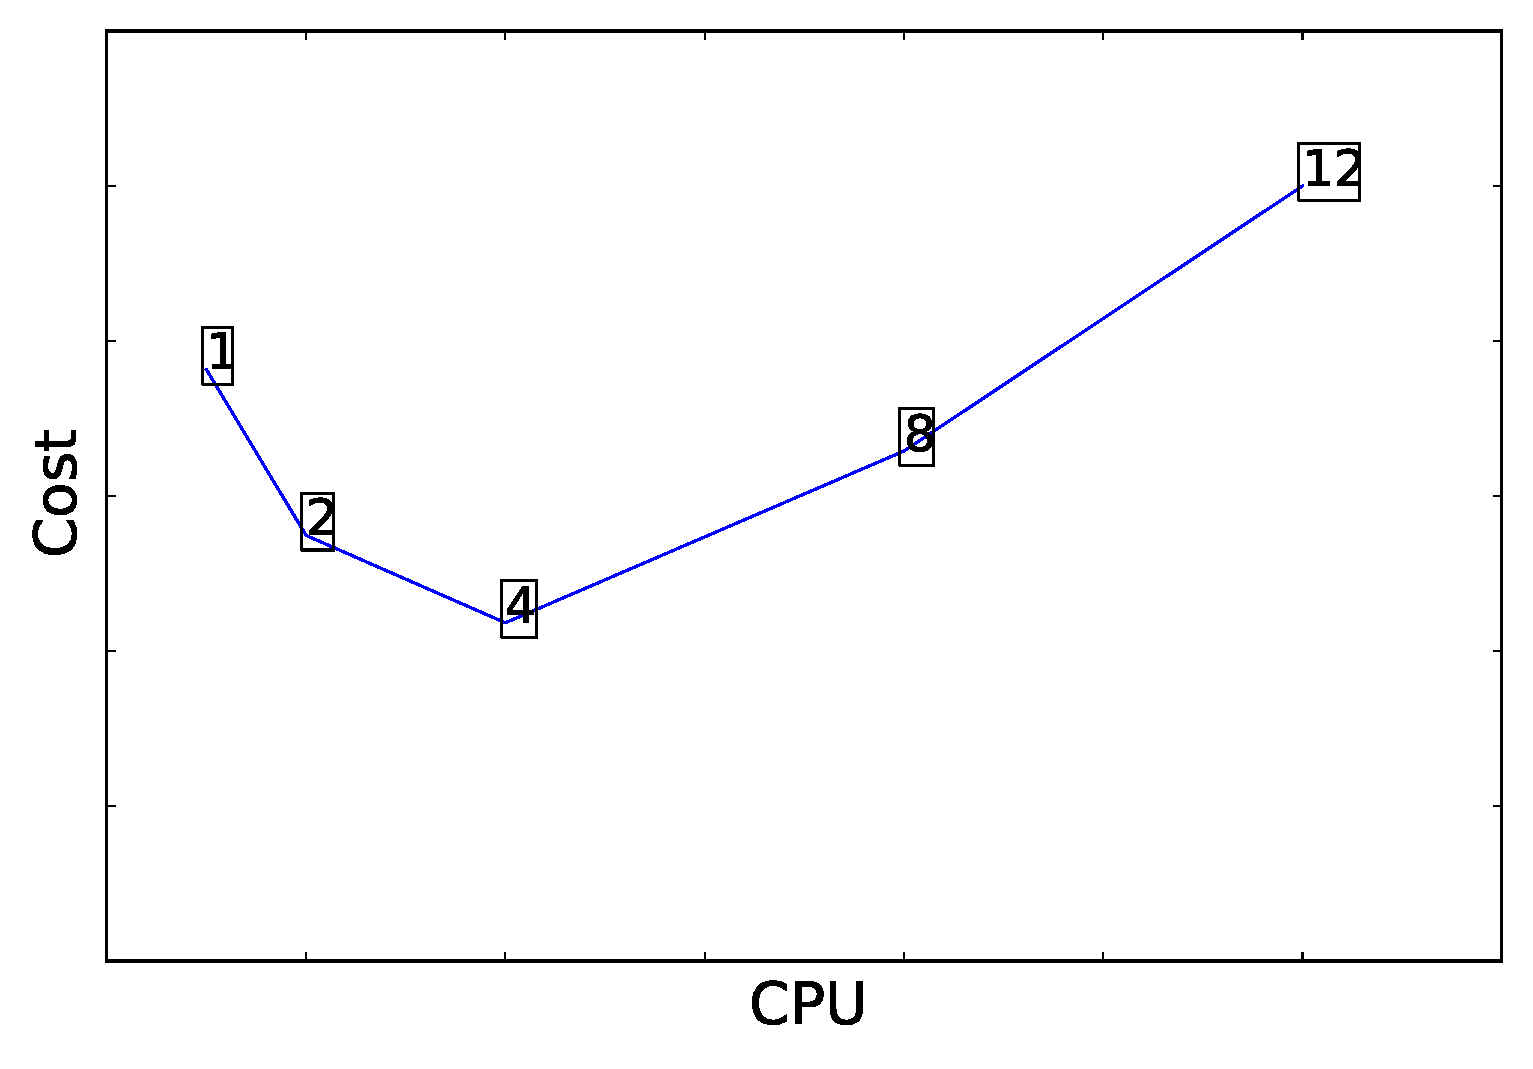
\includegraphics[width=\textwidth]{Chapter-CAT/figures/pagerank_cpu_cost_12_1.eps}
        \caption{PageRank}
        \label{fig:pagerank_cost}
    \end{subfigure}
    \begin{subfigure}[b]{0.3\textwidth}
        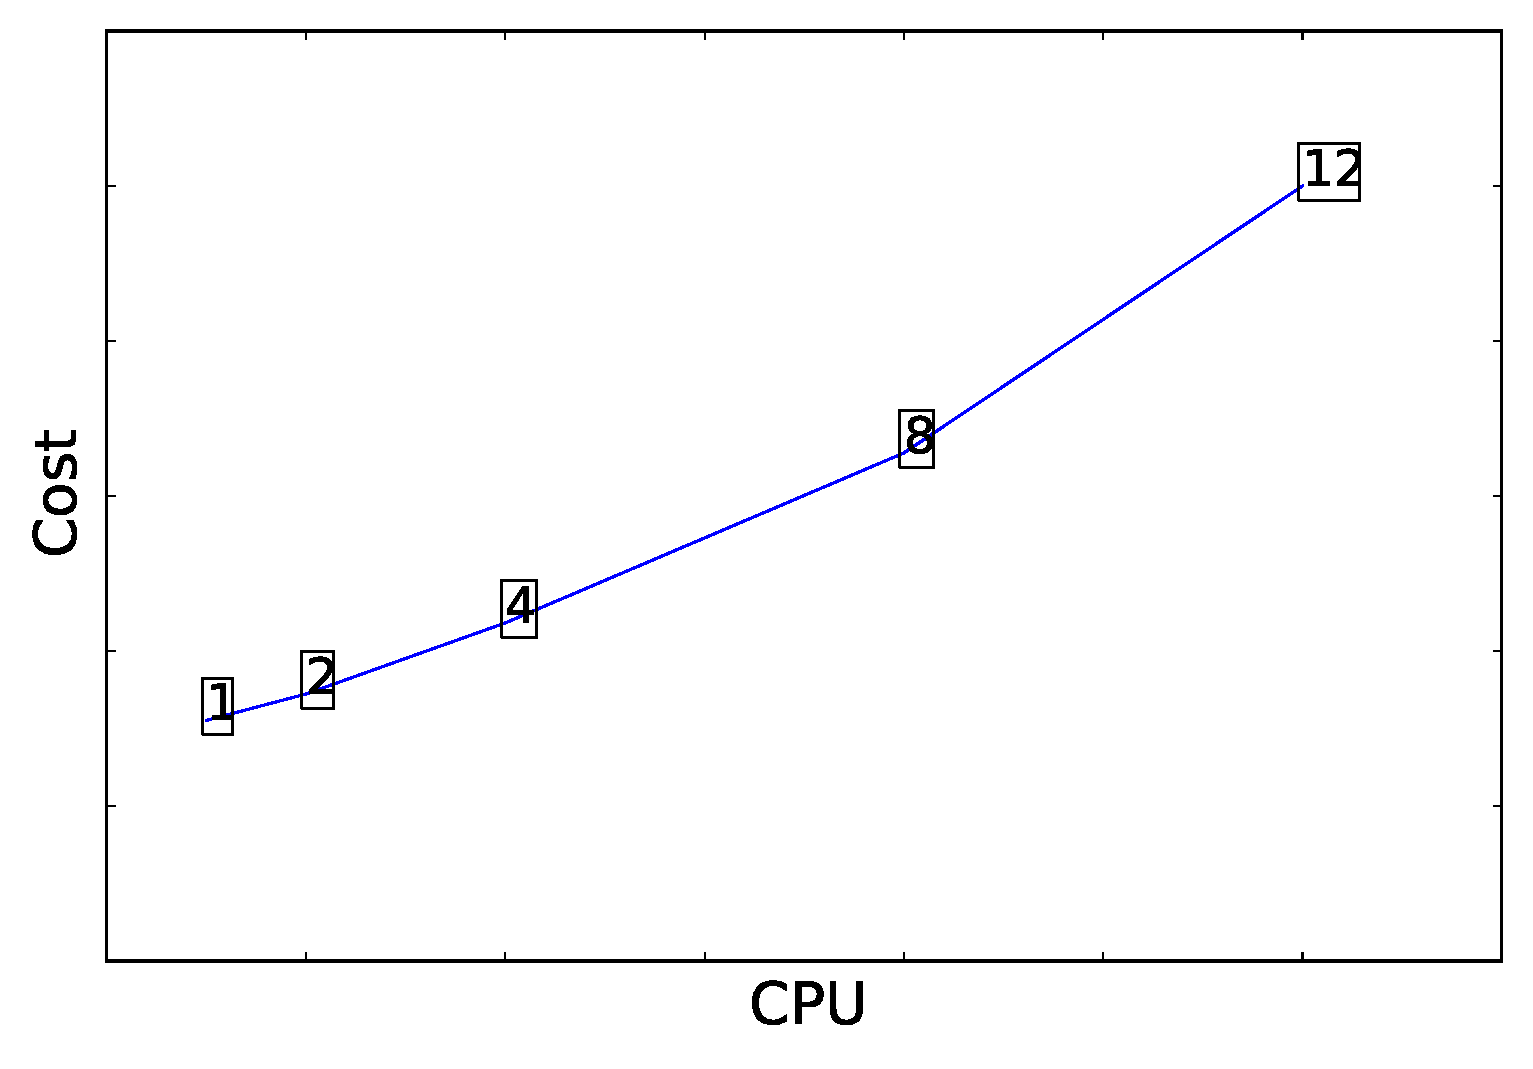
\includegraphics[width=\textwidth]{Chapter-CAT/figures/webloganalysis_cpu_cost_12_1.eps}
        \caption{Web Log Analysis}
        \label{fig:webloganalysis_cost}
    \end{subfigure}
    \begin{subfigure}[b]{0.3\textwidth}
        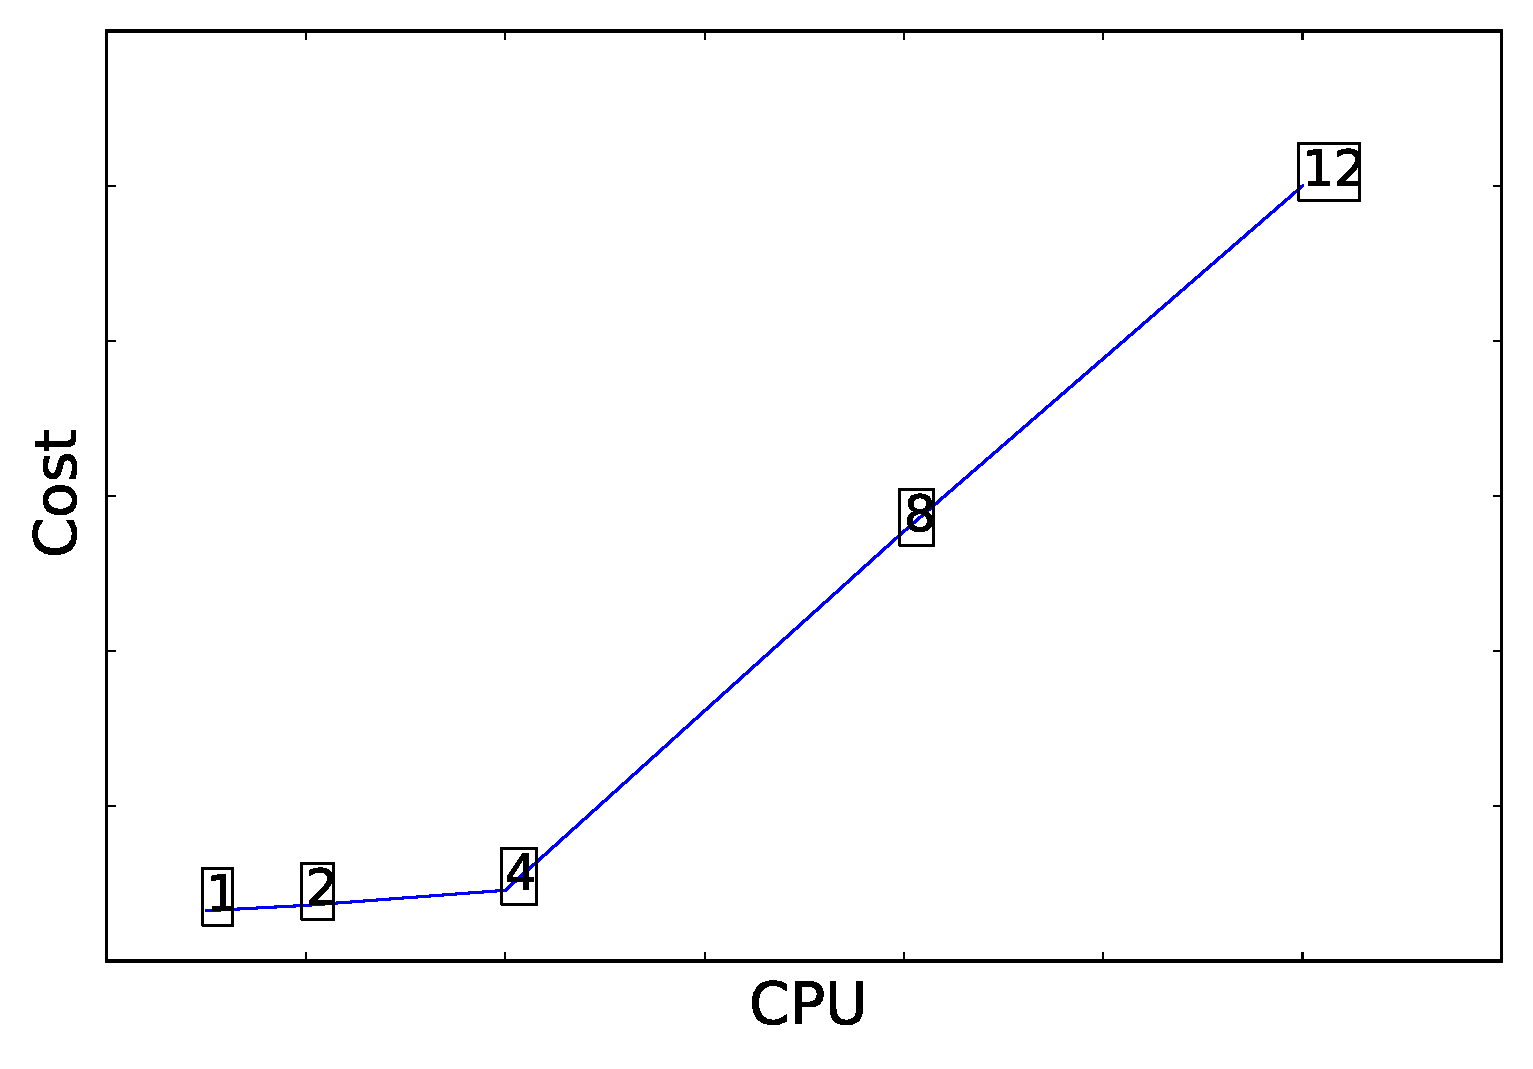
\includegraphics[width=\textwidth]{Chapter-CAT/figures/regression_cpu_cost_12_1.eps}
        \caption{Regression}
        \label{fig:regression_cost}
    \end{subfigure}
    \caption{The speedup and cost saving by CPU scaling (1GB memory per CPU).}
    \label{fig:speed_1gb}
\end{figure}





\iffalse
In this work, we focus on data processing jobs.
We are interested in two metrics:
1) how long to complete a job (execution \textbf{time})
\rone{at}
2) what \textbf{cost}.
Choosing the \emph{best} configuration is not always straightforward because
performance varies both between applications and across configurations within each application.
We run three real-world applications,
\emph{PageRank},
\emph{web log analysis}, and
\emph{regression},
on Apache Spark, a distributed, large-scale data processing system \cite{spark}.
We conduct a series of evaluations of the three applications against
different resource costs by varying
the number of CPUs (from 1 to 12)
and
the size of memory (from 1 to 4 GB per CPU).
We measure the execution time to complete the applications.
\mytable{\ref{table:raw_data}} lists their time and cost in detail.
\myfigure{\ref{fig:application_performance}} uses a scatter plot
to show 
the execution time of applications running against different resource \emph{costs}.
We find that their distribution patterns are not totally alike.
Therefore, there does not exist one best configuration for all applications.
Even within the same applications, execution time can change dramatically.
\myfigure{\ref{fig:application_performance}} also illustrates a convex hull
for outcomes bounded to a subset of the plane.
When choosing the \emph{best} configuration, the solution must be close to the
convex hull.

Finding out the most cost-effective configuration
is difficult for two reasons.
First, execution time is not linearly proportional to resource cost.
In \myfigure{\ref{fig:speed_1gb}}, we show that
the speedup is not linearly increasing with the number of CPUs.
Second, 
application performance is not monotonically increasing or decreasing
with respect to \emph{cost}.
\myfigure{\ref{fig:pagerank_cost}} demonstrates that
the \emph{PageRank} application is more cost-effective with four CPUs
even the cost per unit time is higher.
\emph{cost} is also a function of time.
When the time improvement is enough to compensate the cost increase,
cloud users are more willing to trade cost for time.

Our preliminary evaluation shows only two dimensions of configurations
, CPU and memory.
When it comes to real-world cloud deployment,
users need to figure out the \emph{best} configuration from
a larger dimension.
It is a time-consuming process and it is prone to mis-configuration,
which yields to deadline misses or higher charges.


\begin{table}[!htbp]
\centering
\caption{The execution time and resource cost of applications
running with different numbers of CPUs and memory per CPU.
The text in bold refer to the configurations on the convex hull
in \myfigure{\ref{fig:application_performance}}.}
\label{table:raw_data}
\begin{tabular}{rrrrrrrrr}
\multicolumn{3}{c}{\textbf{Configuration}}  & \multicolumn{2}{c}{\textbf{PageRank}} & \multicolumn{2}{c}{\textbf{Web Log Analysis}} & \multicolumn{2}{c}{\textbf{Regression}}\\
ID  & CPU & Memory/CPU & Time & Cost & Time & Cost & Time & Cost \\ \hline \hline
0   & 1          & 1       & 652.2 & 3261.1  & \textbf{179.3} & \textbf{896.3}  & \textbf{765.0}  & \textbf{3825.2} \\
1   & 1          & 2       & 389.2 & 2335.3  & 220.2 & 1321.1 & 706.7  & 4240.1 \\
2   & 1          & 4       & 267.7 & 2141.8  & 187.8 & 1502.4 & 723.7  & 5789.7 \\
3   & 1          & 8       & 240.3 & 2883.6  & 210.1 & 2521.1 & 701.0  & 8412.0 \\ \hline
4   & 2          & 1       & 234.6 & 2346.3  & \textbf{99.5}  & \textbf{994.6}  & \textbf{423.4}  & \textbf{4233.6} \\
5   & 2          & 2       & \textbf{139.1} & \textbf{1669.1}  & 104.3 & 1252.0 & 433.3  & 5200.1 \\
6   & 2          & 4       & 151.3 & 2420.0  & 123.8 & 1980.1 & 407.8  & 6524.6 \\
7   & 2          & 8       & 152.4 & 3657.0  & 121.6 & 2919.5 & 434.0  & 10414.2 \\ \hline
8   & 4          & 1       & \textbf{93.2}  & \textbf{1864.5}  & \textbf{63.0}  & \textbf{1259.5} & \textbf{269.1}  & \textbf{5382.2} \\
9   & 4          & 2       & 96.2  & 2310.0  & 74.2  & 1781.1 & \textbf{261.7}  & \textbf{6280.3} \\
10  & 4          & 4       & 95.7  & 3063.2  & 71.0  & 2270.8 & 268.7  & 8598.7 \\
11  & 4          & 8       & 101.0 & 4846.5  & 68.0  & 3262.1 & 275.9  & 13242.1 \\ \hline
12  & 8          & 1       & \textbf{70.3}  & \textbf{2811.5}  & \textbf{47.3}  & \textbf{1892.5} & 817.8  & 32711.8 \\
13  & 8          & 2       & 72.4  & 3475.4  & 47.5  & 2277.8 & 842.3  & 40431.1 \\
14  & 8          & 4       & 75.4  & 4828.5  & 55.0  & 3515.8 & 711.2  & 45518.7 \\
15  & 8          & 8       & 70.7  & 6783.4  & 46.8  & 4488.7 & 692.7  & 66502.3 \\ \hline
16  & 12         & 1       & 71.2  & 4272.9  & 48.1  & 2887.0 & 983.5  & 59007.1 \\
17  & 12         & 2       & \textbf{69.6}  & \textbf{5007.7}  & \textbf{46.0}  & \textbf{3309.2} & 1043.4 & 75122.3 \\
18  & 12         & 4       & 72.0  & 6912.8  & \textbf{45.4}  & \textbf{4357.1} & 1026.6 & 98549.5 \\
19  & 12         & 8       & 73.7  & 10617.9 & 49.9  & 7180.6 & 940.0  & 135362.0
\end{tabular}
\end{table}






\begin{figure}
	\captionsetup{justification=centering}
    \centering
	\begin{subfigure}[b]{0.3\textwidth}
        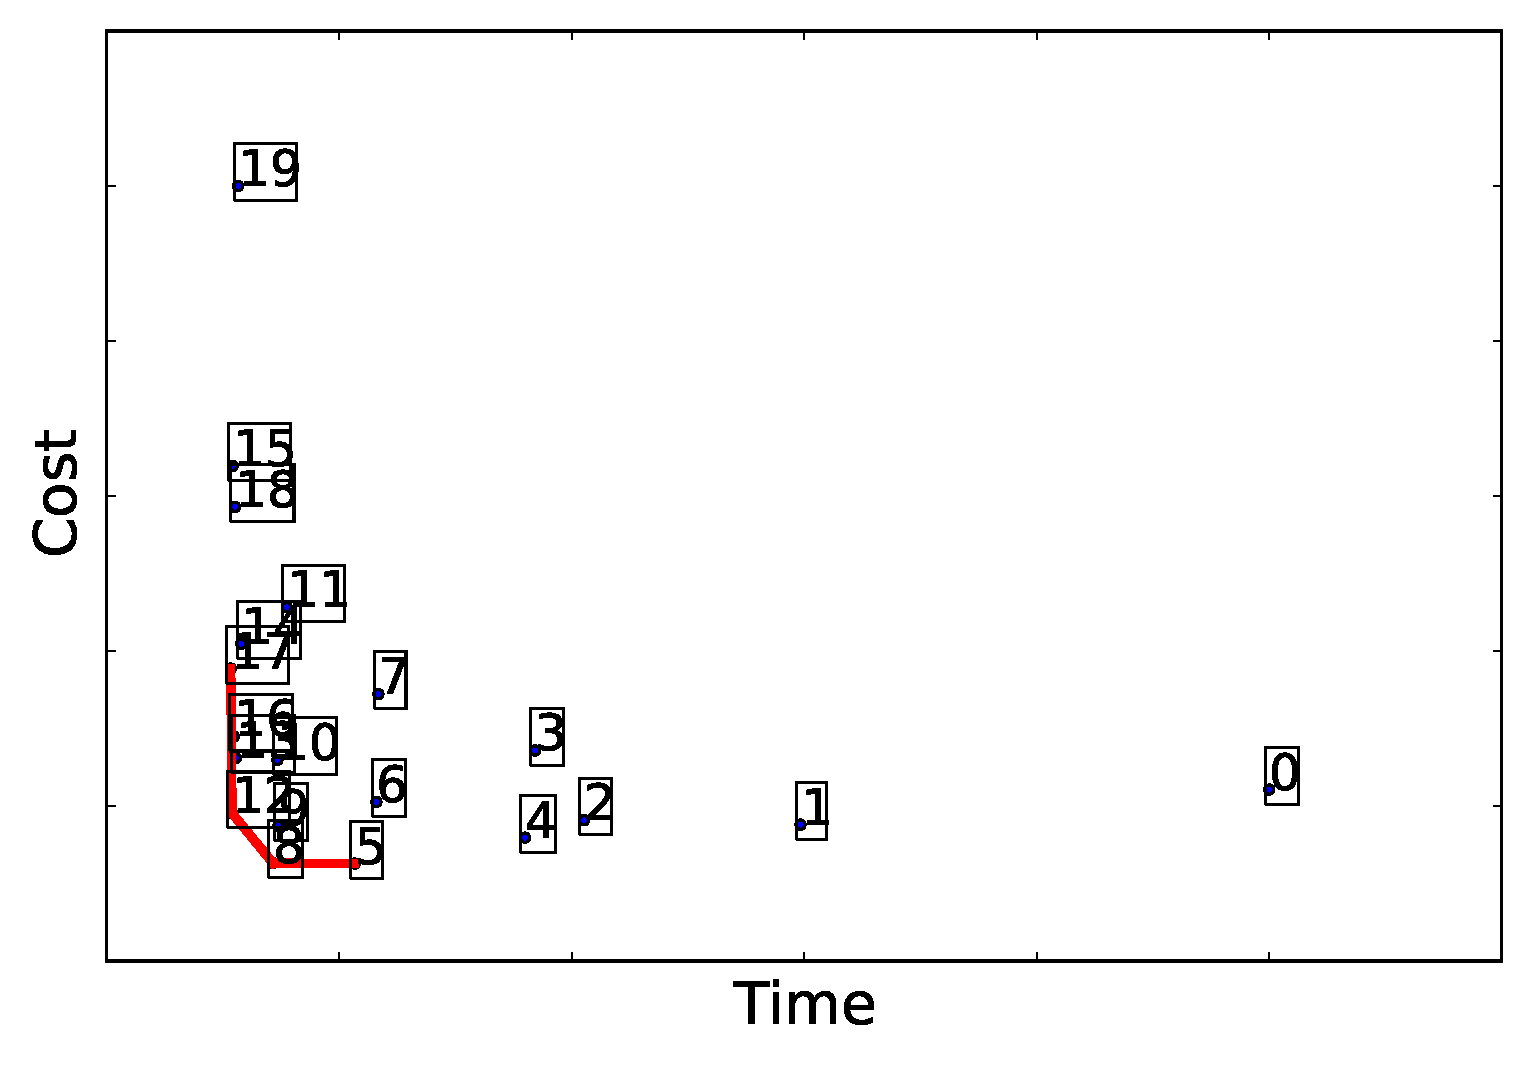
\includegraphics[width=\textwidth]{Chapter-CAT/figures/pagerank_elapsed_cost_all_frontier.eps}
        \caption{PageRank}
        \label{fig:pagerank_configurations}
    \end{subfigure}
    \begin{subfigure}[b]{0.3\textwidth}
        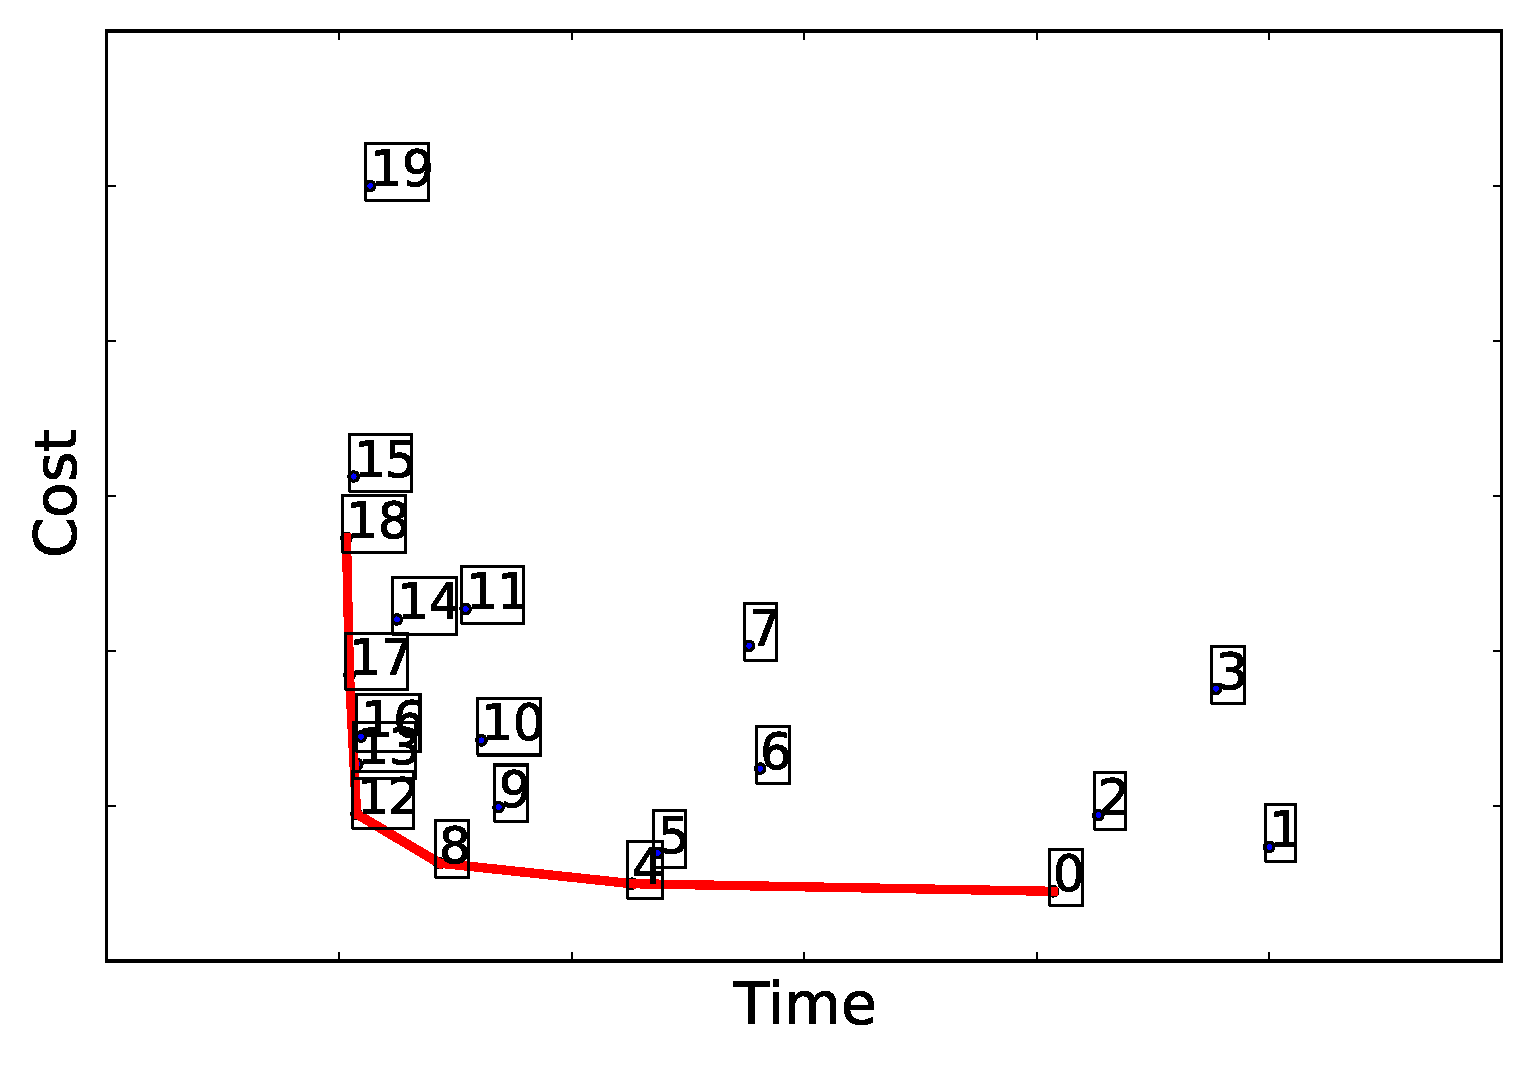
\includegraphics[width=\textwidth]{Chapter-CAT/figures/webloganalysis_elapsed_cost_all_frontier.eps}
        \caption{Web Log Analysis}
        \label{fig:webloganalysis_configurations}
    \end{subfigure}
    \begin{subfigure}[b]{0.3\textwidth}
        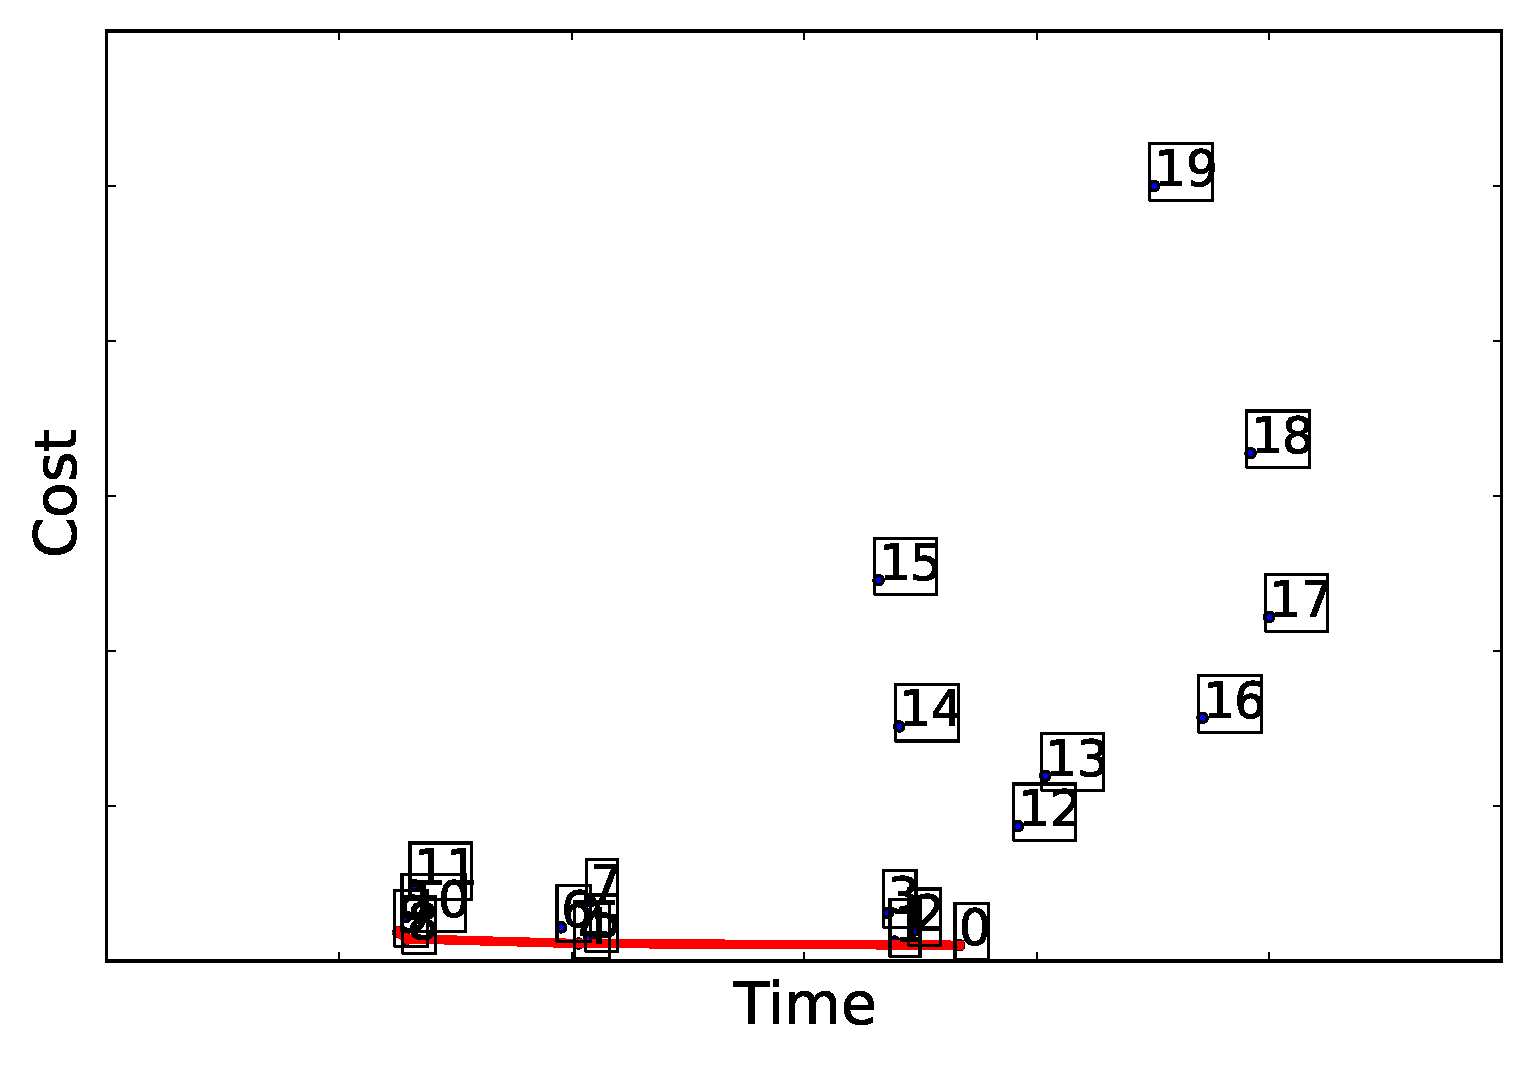
\includegraphics[width=\textwidth]{Chapter-CAT/figures/regression_elapsed_cost_all_frontier.eps}
        \caption{Regression}
        \label{fig:regression_configurations}
    \end{subfigure}
    \caption{Applications' execution time and resource costs with different configurations.}
    \label{fig:application_performance}
\end{figure}


\begin{figure}
	\captionsetup{justification=centering}
    \centering
	\begin{subfigure}[b]{0.3\textwidth}
        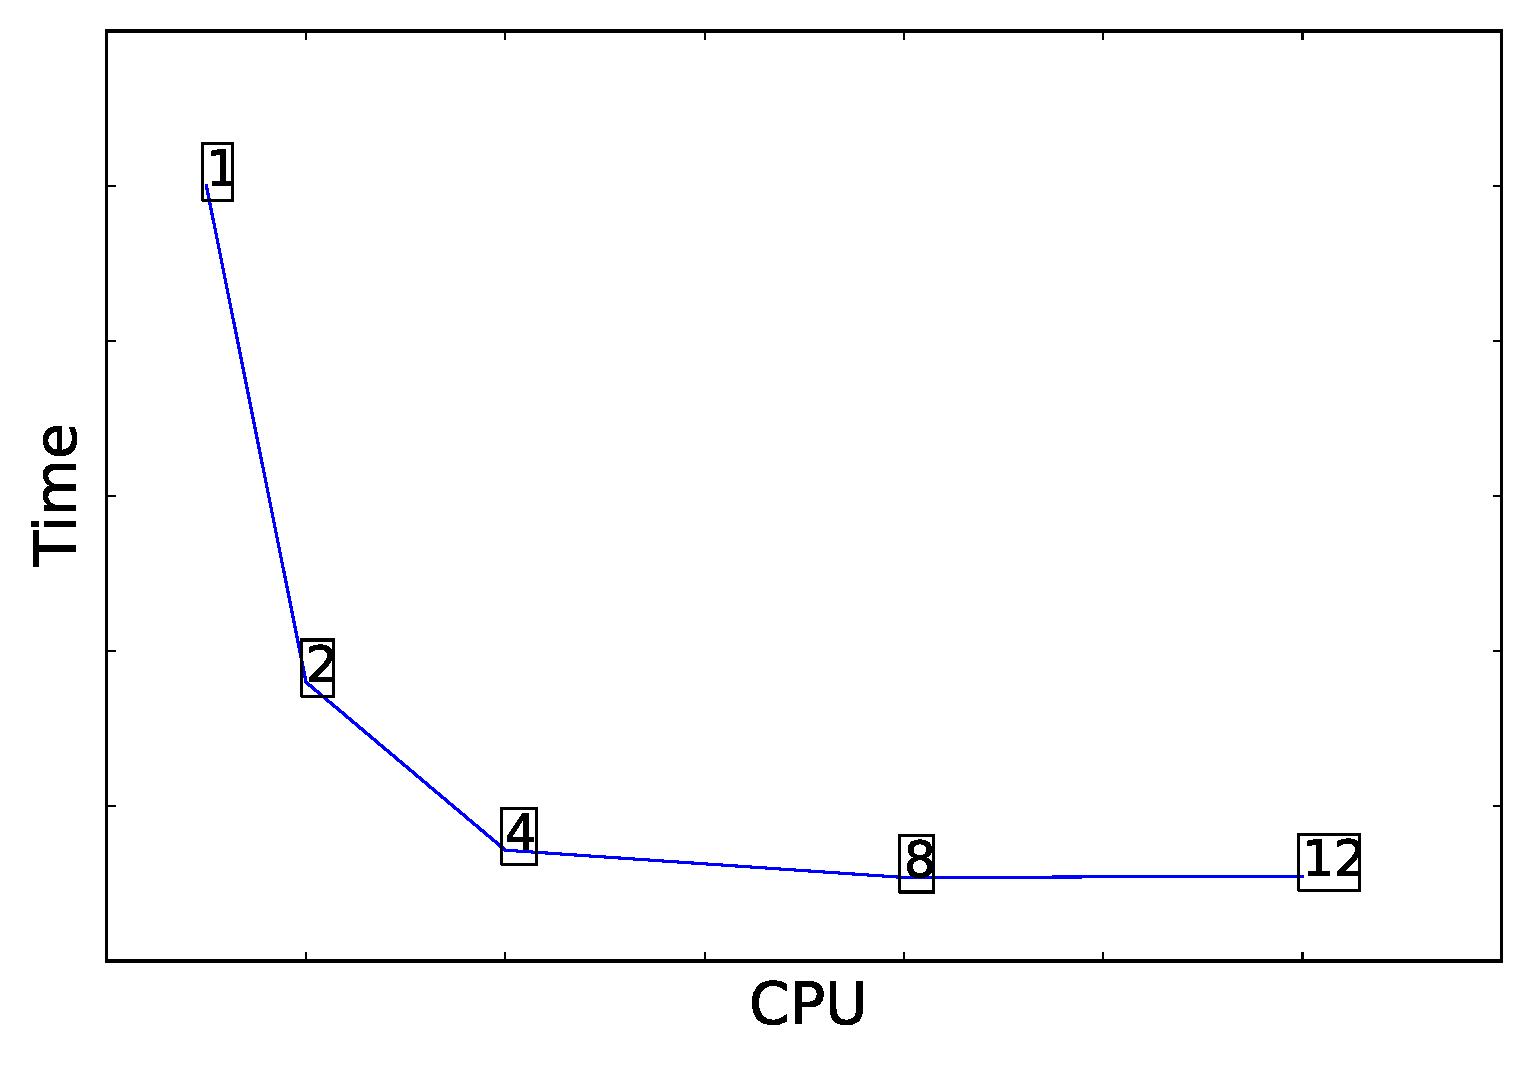
\includegraphics[width=\textwidth]{Chapter-CAT/figures/pagerank_cpu_elapsed_12_1.eps}
        \caption{PageRank}
        \label{fig:pagerank_time}
    \end{subfigure}
    \begin{subfigure}[b]{0.3\textwidth}
        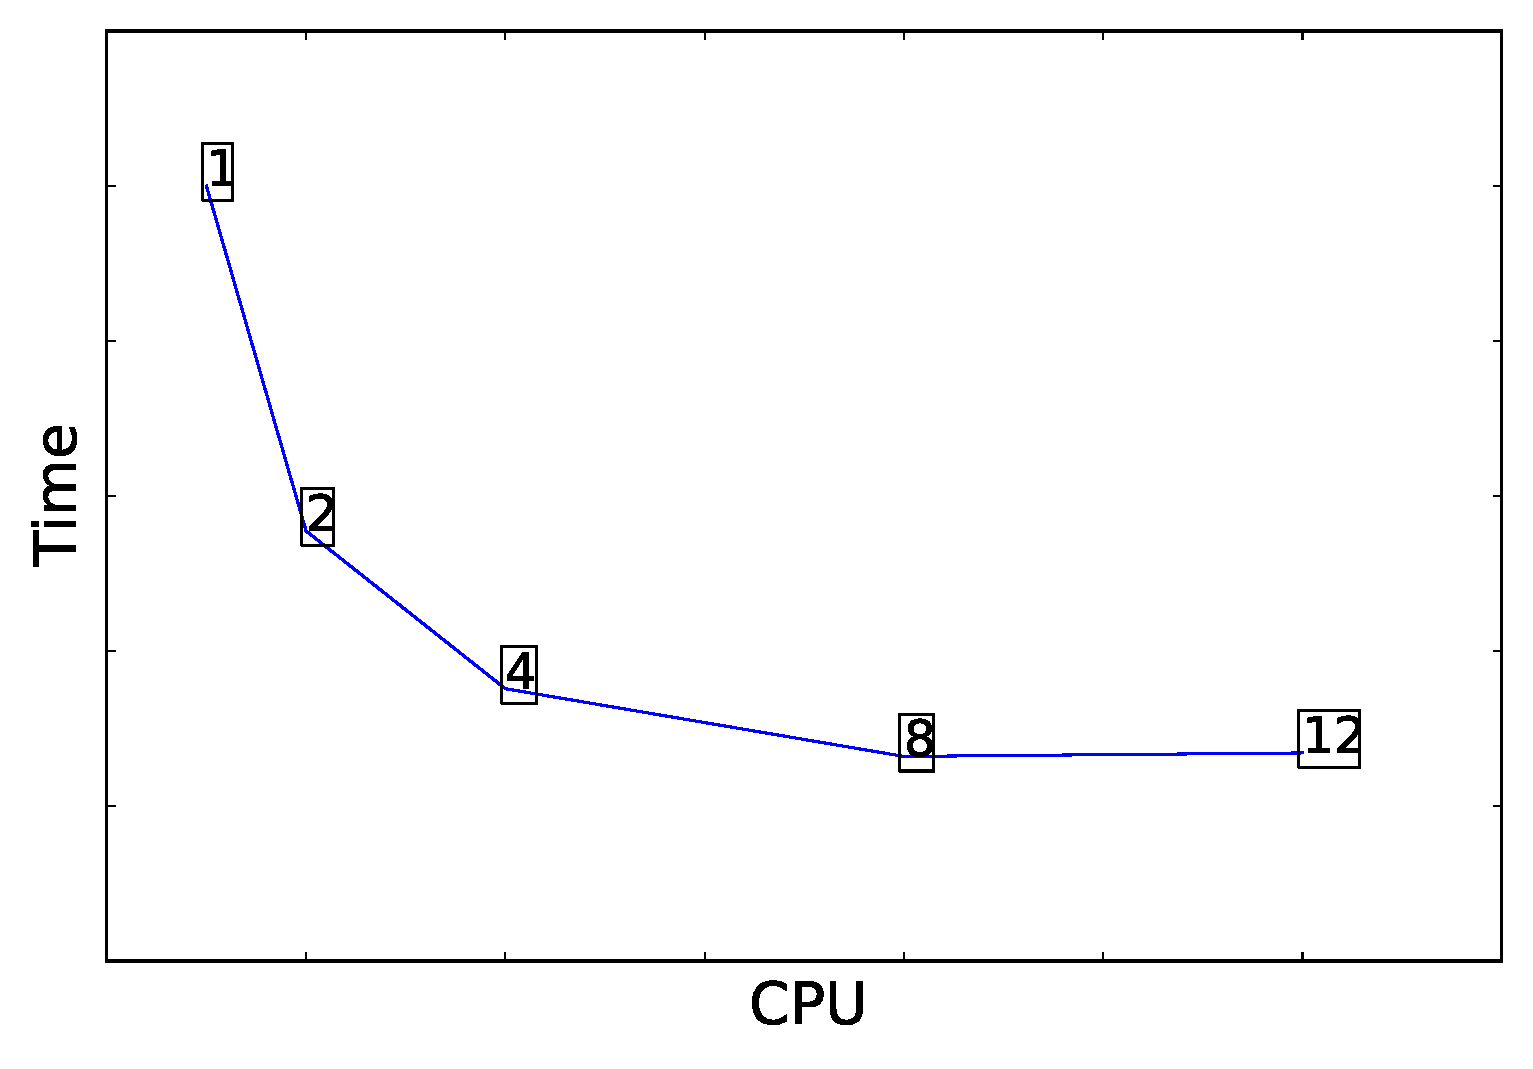
\includegraphics[width=\textwidth]{Chapter-CAT/figures/webloganalysis_cpu_elapsed_12_1.eps}
        \caption{Web Log Analysis}
        \label{fig:webloganalysis_time}
    \end{subfigure}
    \begin{subfigure}[b]{0.3\textwidth}
        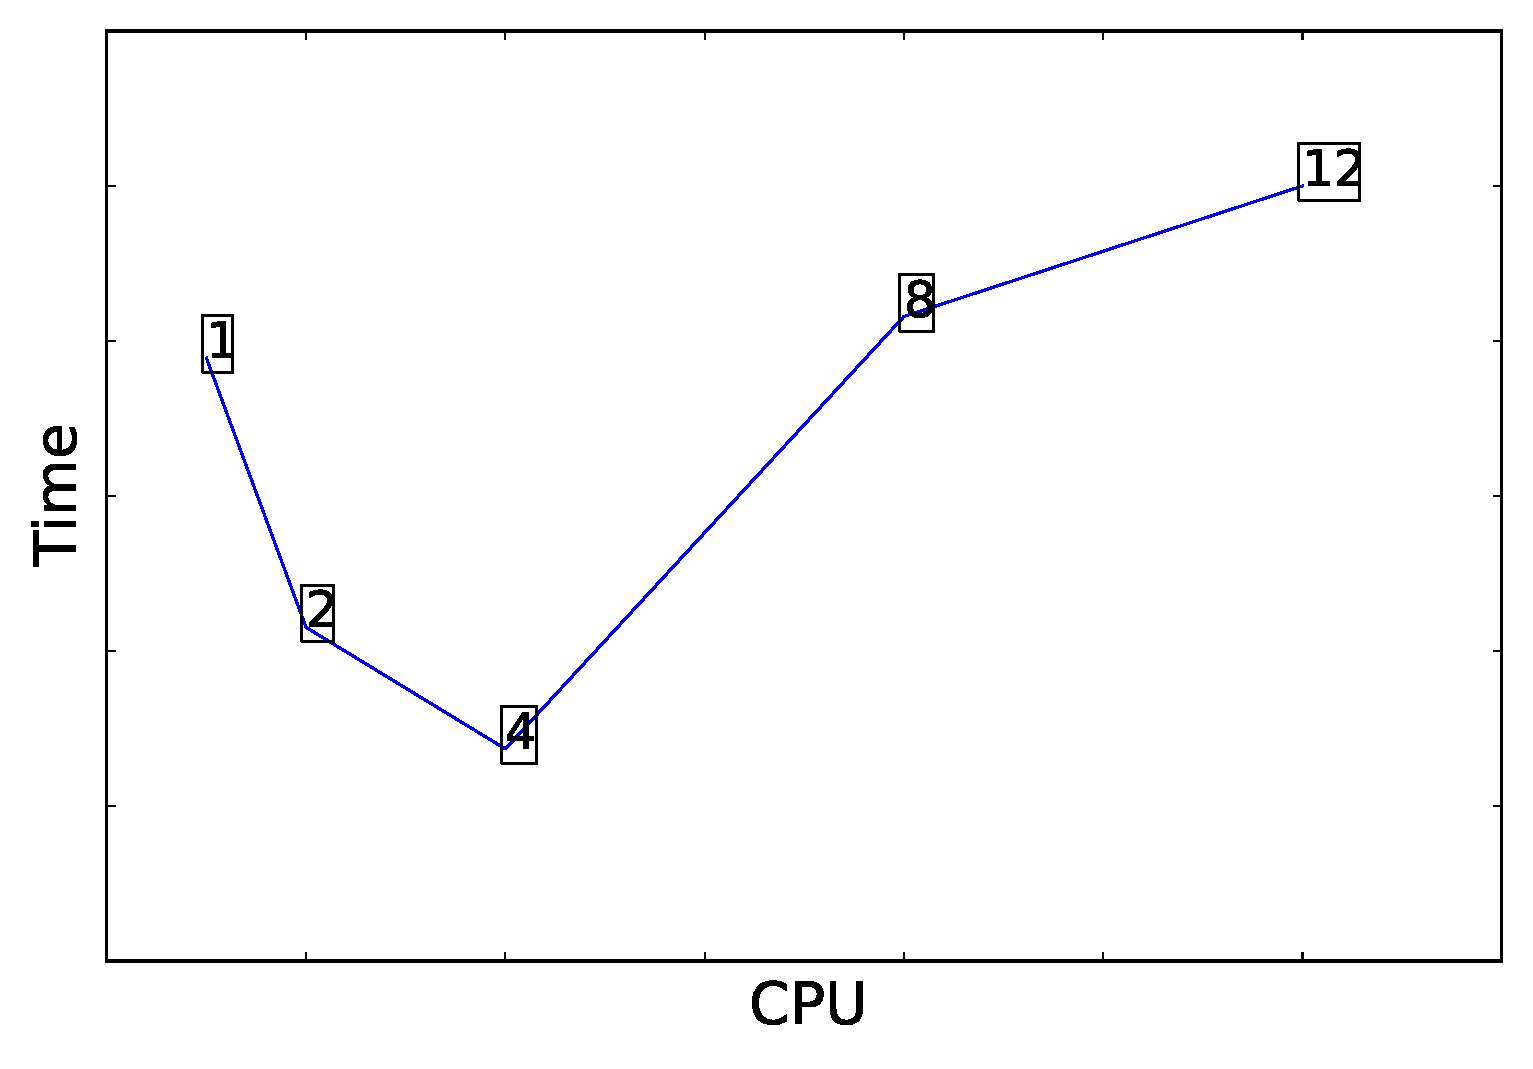
\includegraphics[width=\textwidth]{Chapter-CAT/figures/regression_cpu_elapsed_12_1.eps}
        \caption{Regression}
        \label{fig:regression_time}
    \end{subfigure}
    \bigskip
    \begin{subfigure}[b]{0.3\textwidth}
        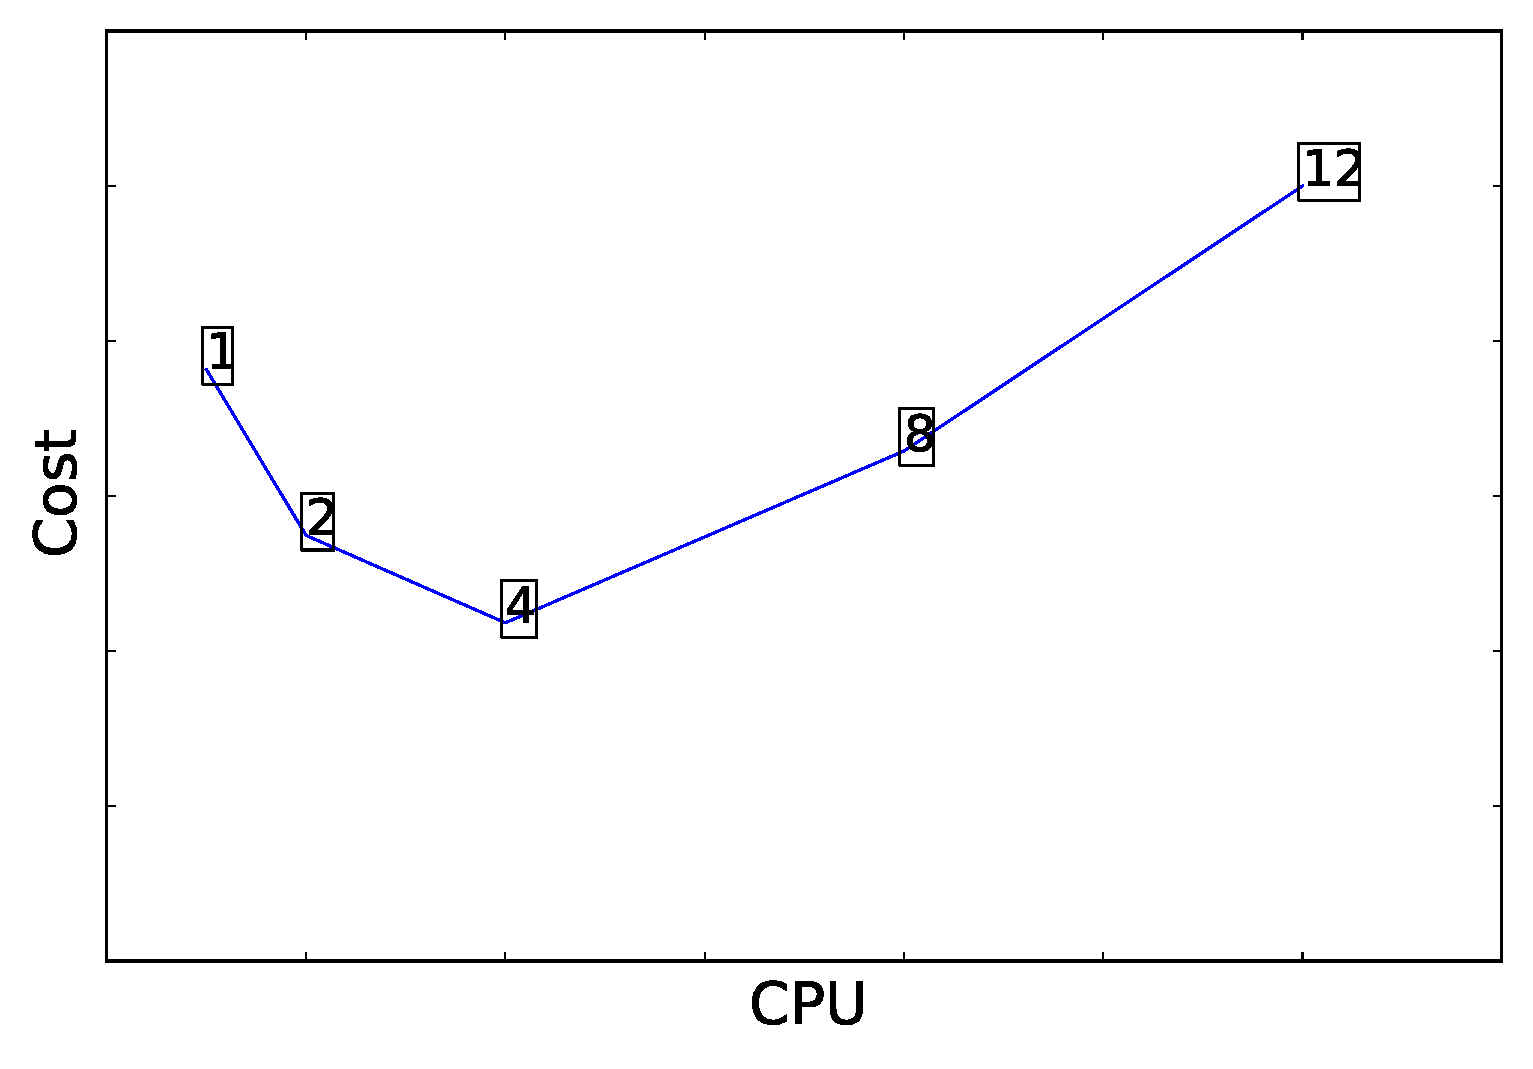
\includegraphics[width=\textwidth]{Chapter-CAT/figures/pagerank_cpu_cost_12_1.eps}
        \caption{PageRank}
        \label{fig:pagerank_cost}
    \end{subfigure}
    \begin{subfigure}[b]{0.3\textwidth}
        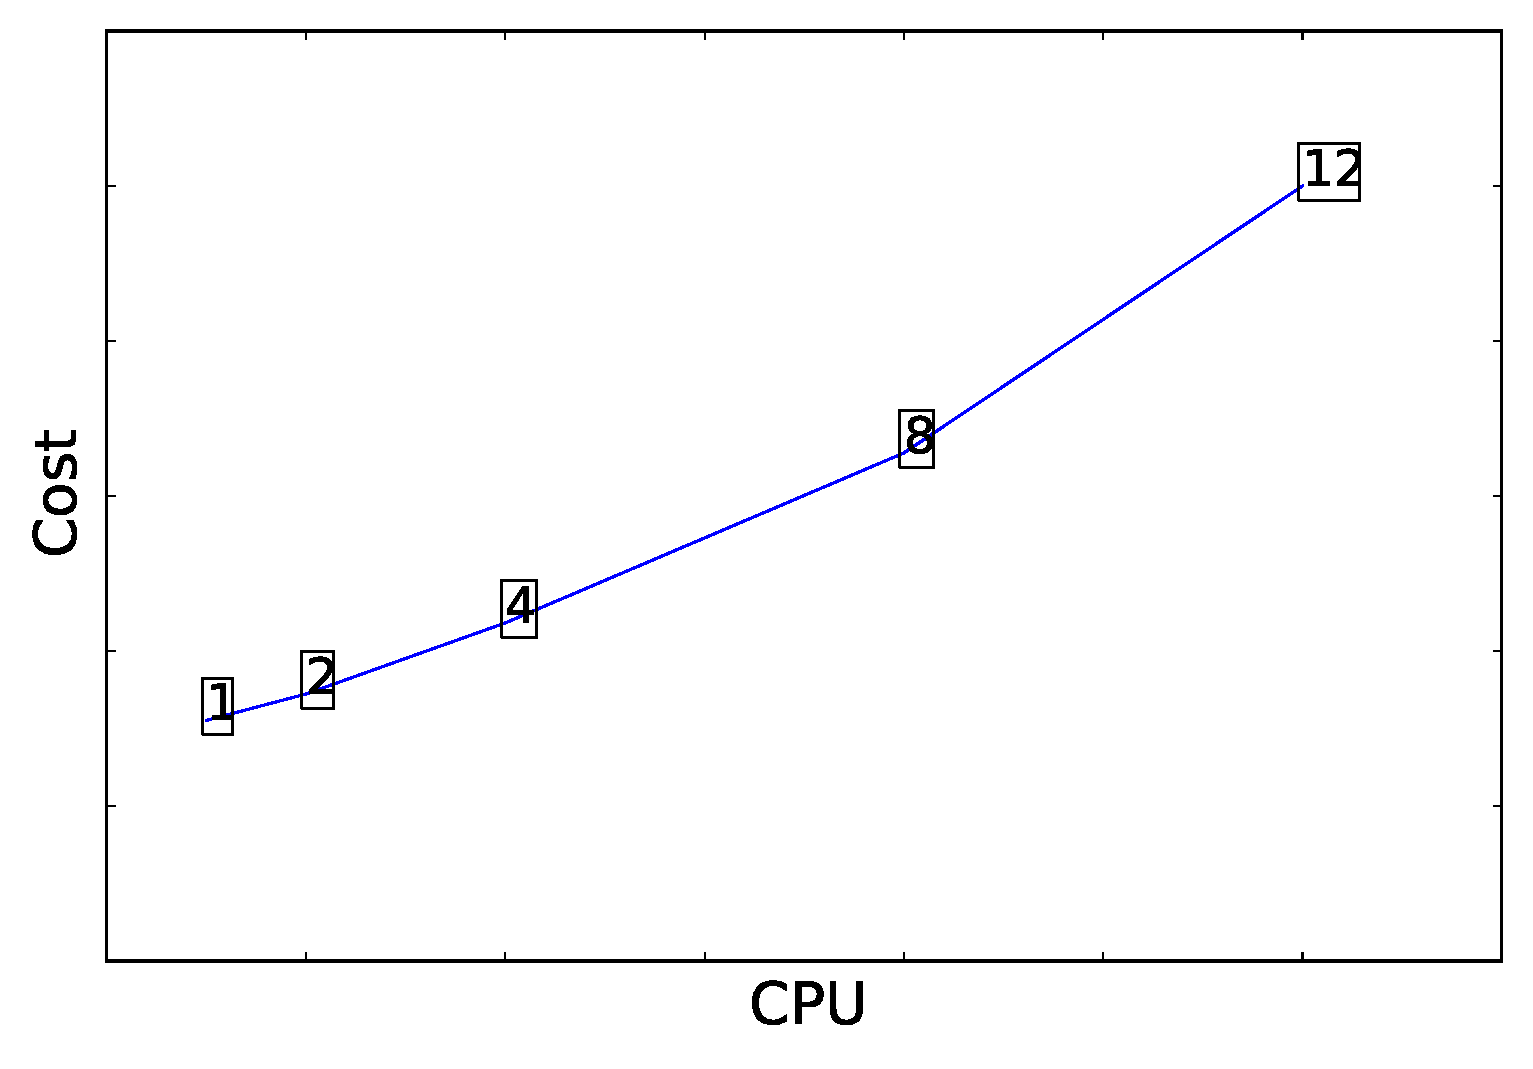
\includegraphics[width=\textwidth]{Chapter-CAT/figures/webloganalysis_cpu_cost_12_1.eps}
        \caption{Web Log Analysis}
        \label{fig:webloganalysis_cost}
    \end{subfigure}
    \begin{subfigure}[b]{0.3\textwidth}
        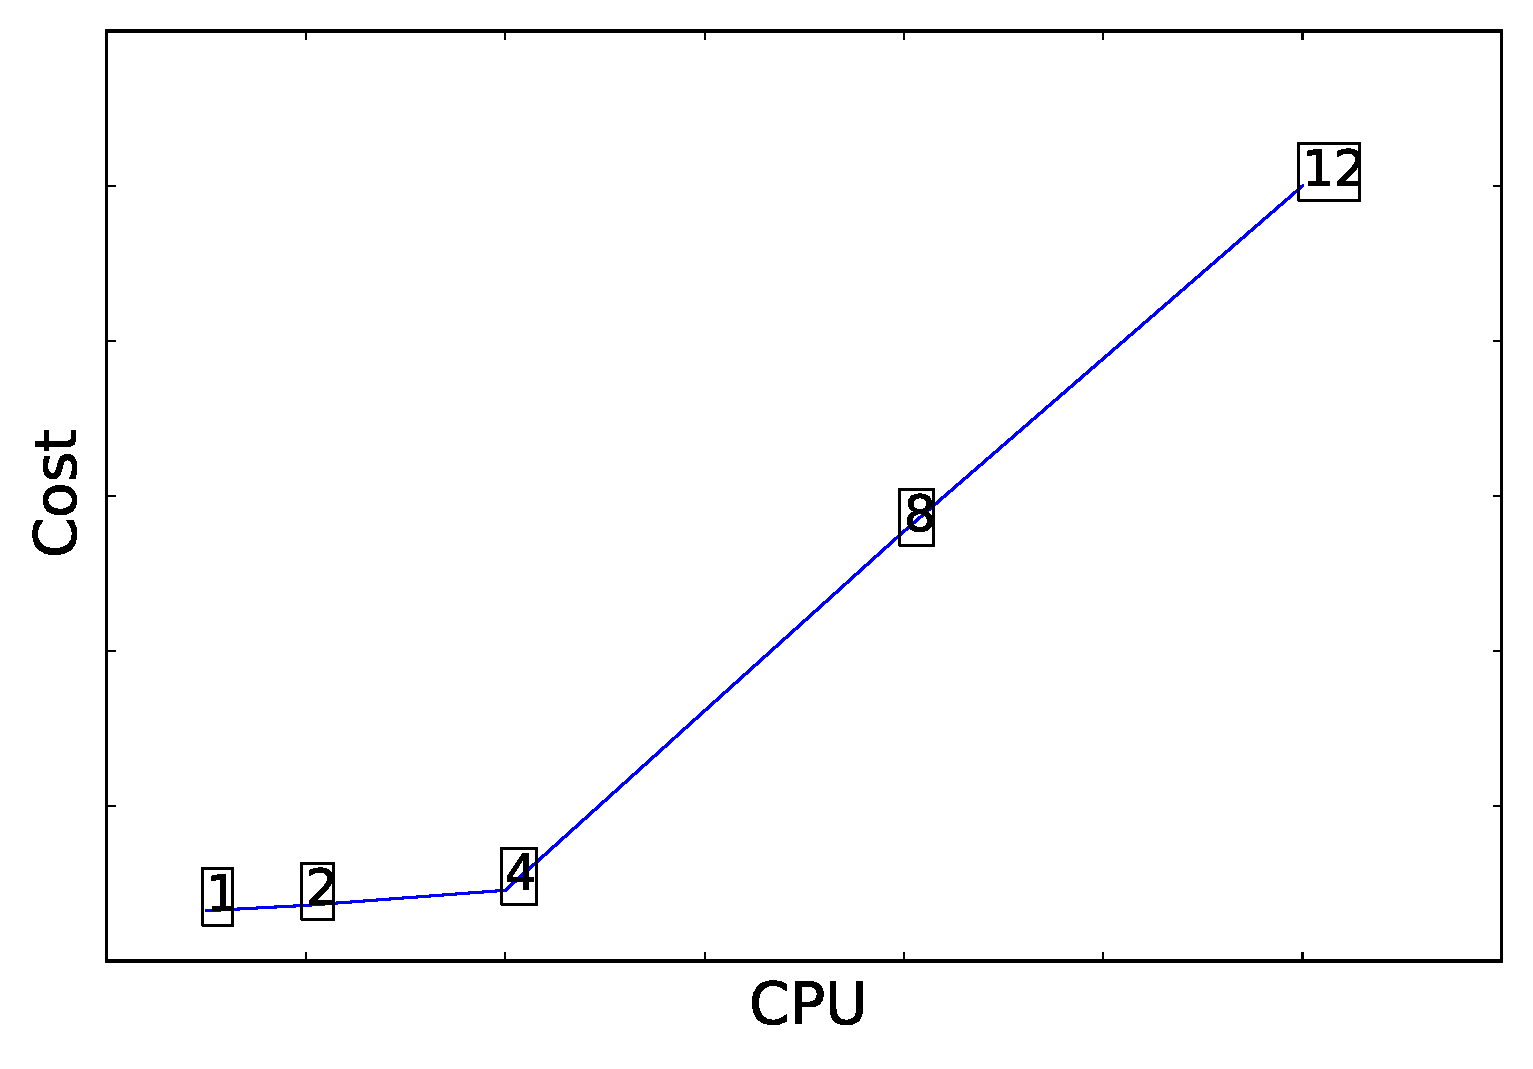
\includegraphics[width=\textwidth]{Chapter-CAT/figures/regression_cpu_cost_12_1.eps}
        \caption{Regression}
        \label{fig:regression_cost}
    \end{subfigure}
    \caption{The speedup and cost saving by CPU scaling (1GB memory per CPU).}
    \label{fig:speed_1gb}
\end{figure}


\paragraph*{Cost-Delay Product (CDP)}

When hosting data-intensive applications on the cloud,
users can choose the \emph{fastest} configuration regardless of cost
or the \emph{cheapest} configuration without the time constraint.
Neither choice is truly piratical.
There is always a trade-off between \emph{time} and \emph{cost}.
Users are willing to spend more on resources when
time is more critical (hard deadline) or
the increase in cost expects reasonable decrease in execution time (soft deadline).
Similarly, when the time constraint is relaxed, users accept
slower configuration but with higher cost saving.

We propose using cost-delay product (CDP),
similar to energy-delay product (EDP)~\cite{Freeh2007},
to analyze the trade-offs
for choosing the cloud configurations of data-intensive applications.
CDP puts the same importance on time and cost.
For example,
a $5\%$ slow down in execution time
is enough to justify
a $5\%$ cost saving.
$CD^2P$ and $C^2DP$, on the other hand, shift the importance to
time and cost respectively.
When the time improvement is $1\%$ but it incurs $50\%$ increase in cost,
users will probably choose the slower configuration.
In the PageRank case, for example,
users are more likely to choose four CPUs instead of eight CPUs because
25\% reduction in execution time requires
more than 50\% extra cost.
We explain the three applications' trade-off as follows.

\subparagraph*{PageRank}

PageRank is an ranking algorithm to calculate the importance of website pages
by counting the number of links to them.
Our evaluation has shown that execution time decreases as
we increase the number of CPUs.
Although \emph{PageRank} exhibits shorter execution time
when the CPU count is greater than eight,
it more makes sense to choose four CPUs as it is more cost effective,
as depicted in~\myfigure{\ref{fig:pagerank_cost}}.
However, when time is more critical ($CD^2P$),
~\myfigure{\ref{fig:pagerank_time}} shows that
eight CPUs is a better choice.

\subparagraph*{Web Log Analysis}
This application tracks the query counts and aggregate bytes in a particular group.
The CPU count greatly affects the execution time but memory size does not
show significant impact.
As shown in~\myfigure{\ref{fig:webloganalysis_time}}, a larger number of CPUs (increasing from 1 to 4)
increase resource costs but time reduction is large enough
to compensate the increase in cost.
This is not the case when the CPU count is more than four.
When time is more critical, $CD^2P$ suggests eight CPUs is a viable configuration.

\subparagraph*{Regression}
The regression application generates a function that estimates 
the relationships among variables.
Different from the above two applications, \emph{regression} shows
more CPU counts do no necessarily help reduce execution time.
It is even worse.
One possible explanation is the overhead by increasing parallelism overcomes
the benefits by higher parallelism.


\iffalse
\begin{figure}
	\captionsetup{justification=centering}
    \centering
	\begin{subfigure}[b]{0.3\textwidth}
        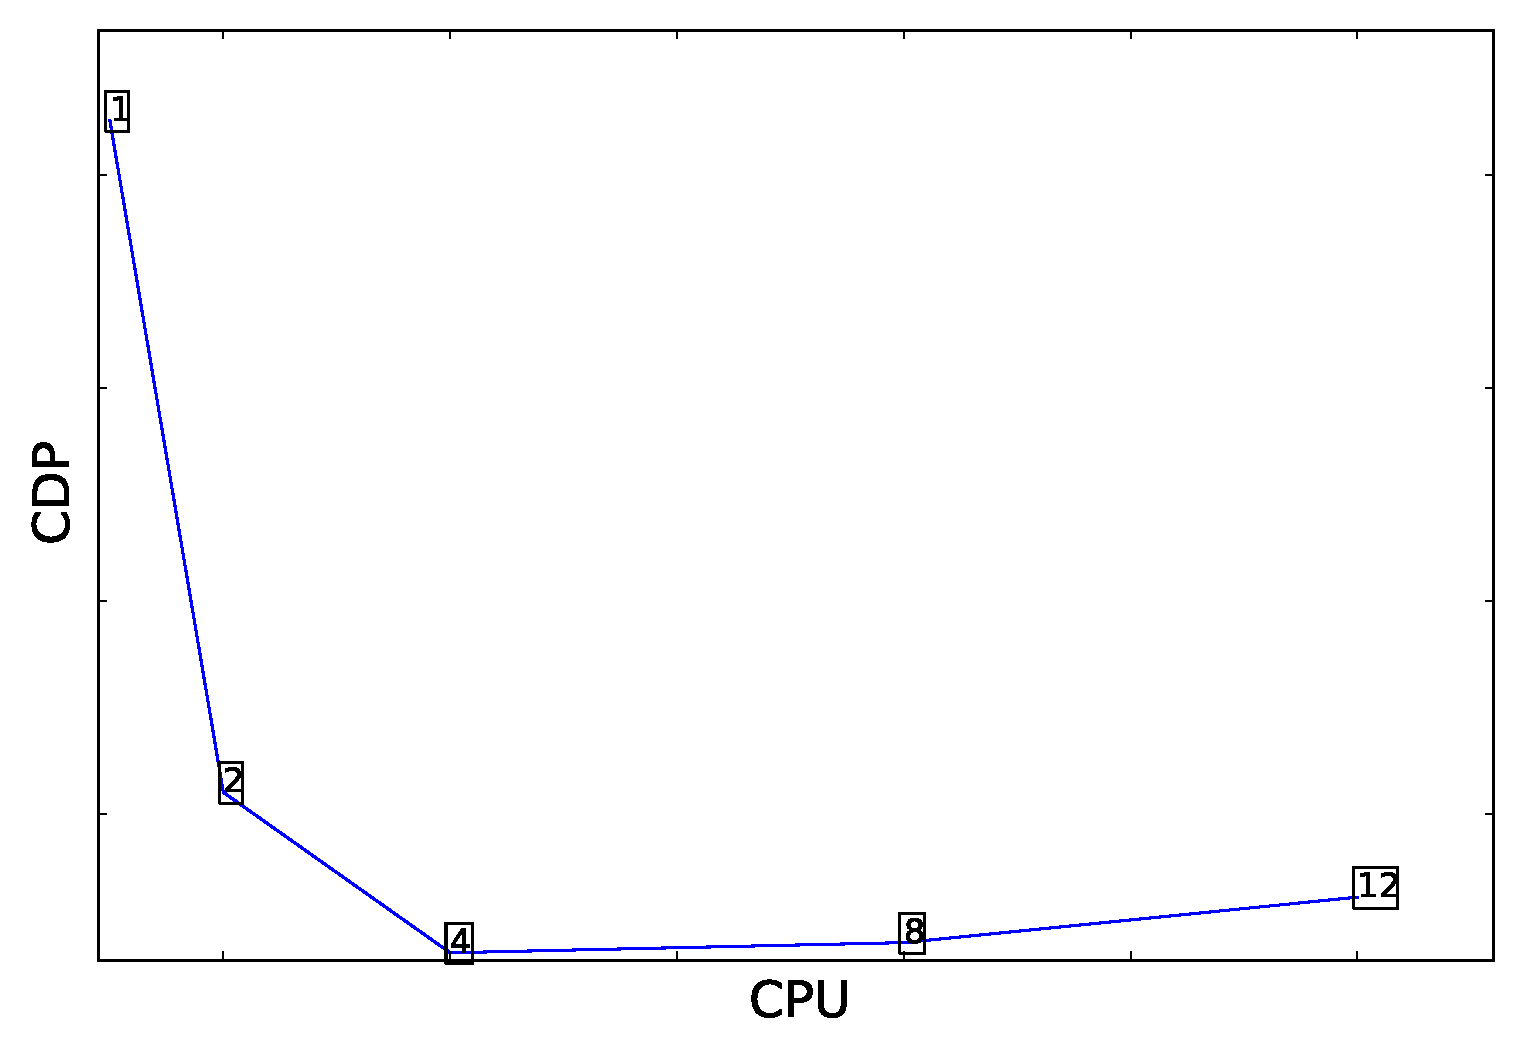
\includegraphics[width=\textwidth]{Chapter-8/figures/pagerank_cpu_CDP_12_1.eps}
        \caption{PageRank}
        \label{fig:pagerank_cdp}
    \end{subfigure}
    \begin{subfigure}[b]{0.3\textwidth}
        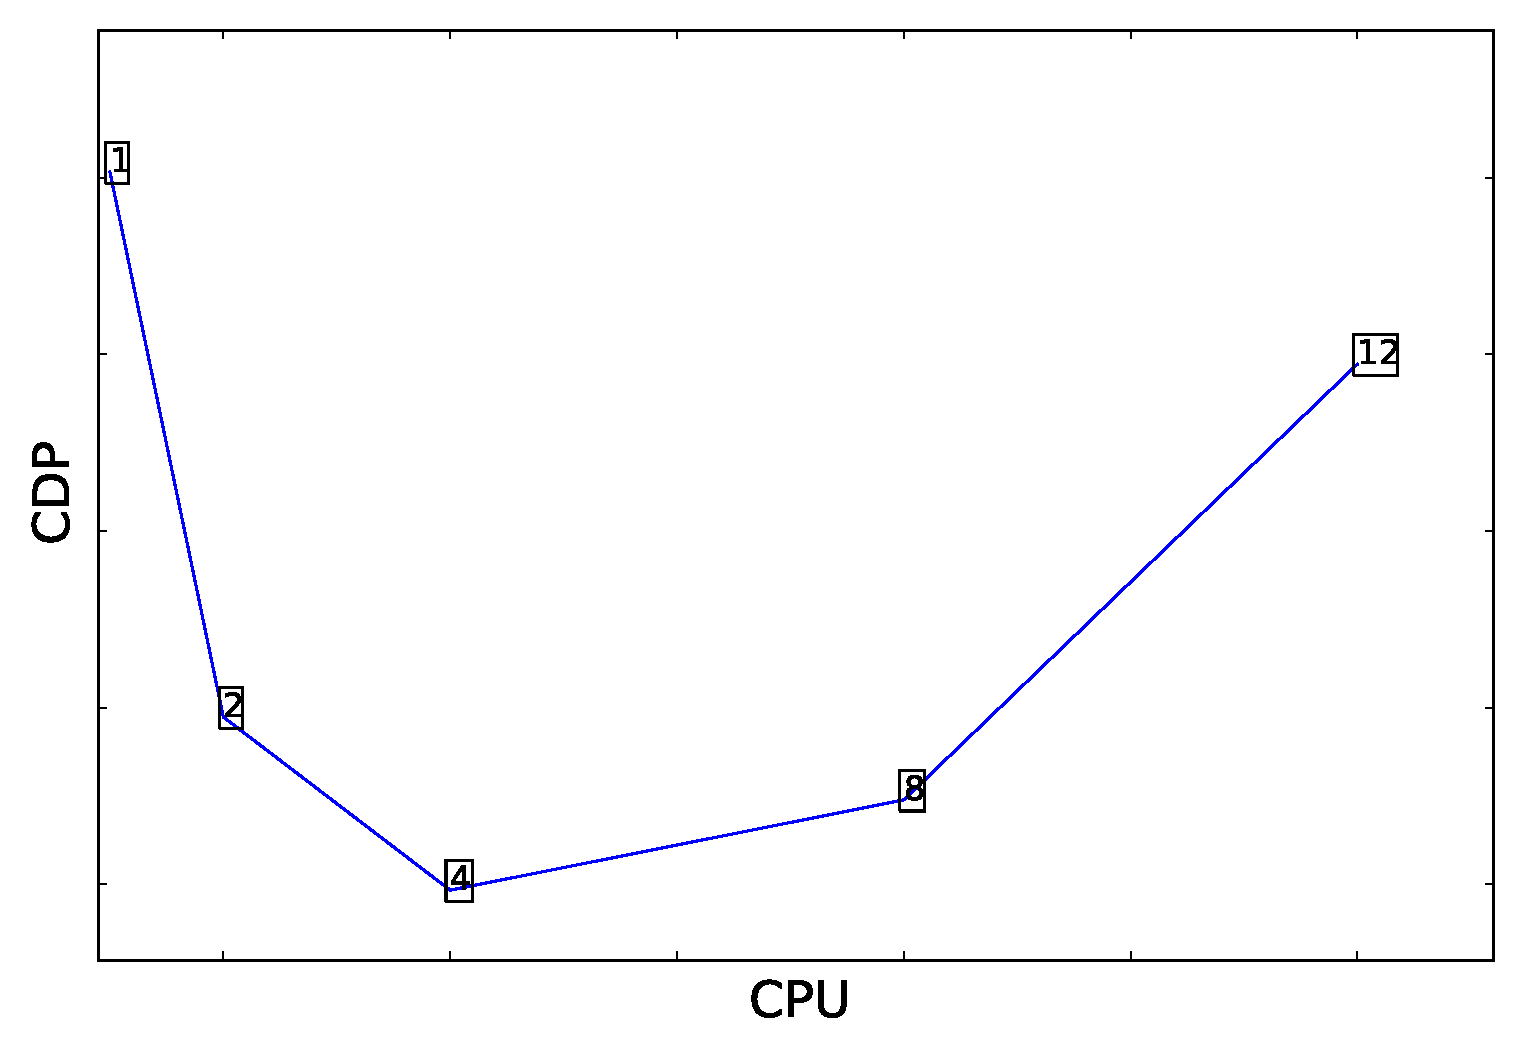
\includegraphics[width=\textwidth]{Chapter-8/figures/webloganalysis_cpu_CDP_12_1.eps}
        \caption{Web Log Analysis}
        \label{fig:webloganalysis_cdp}
    \end{subfigure}
    \begin{subfigure}[b]{0.3\textwidth}
        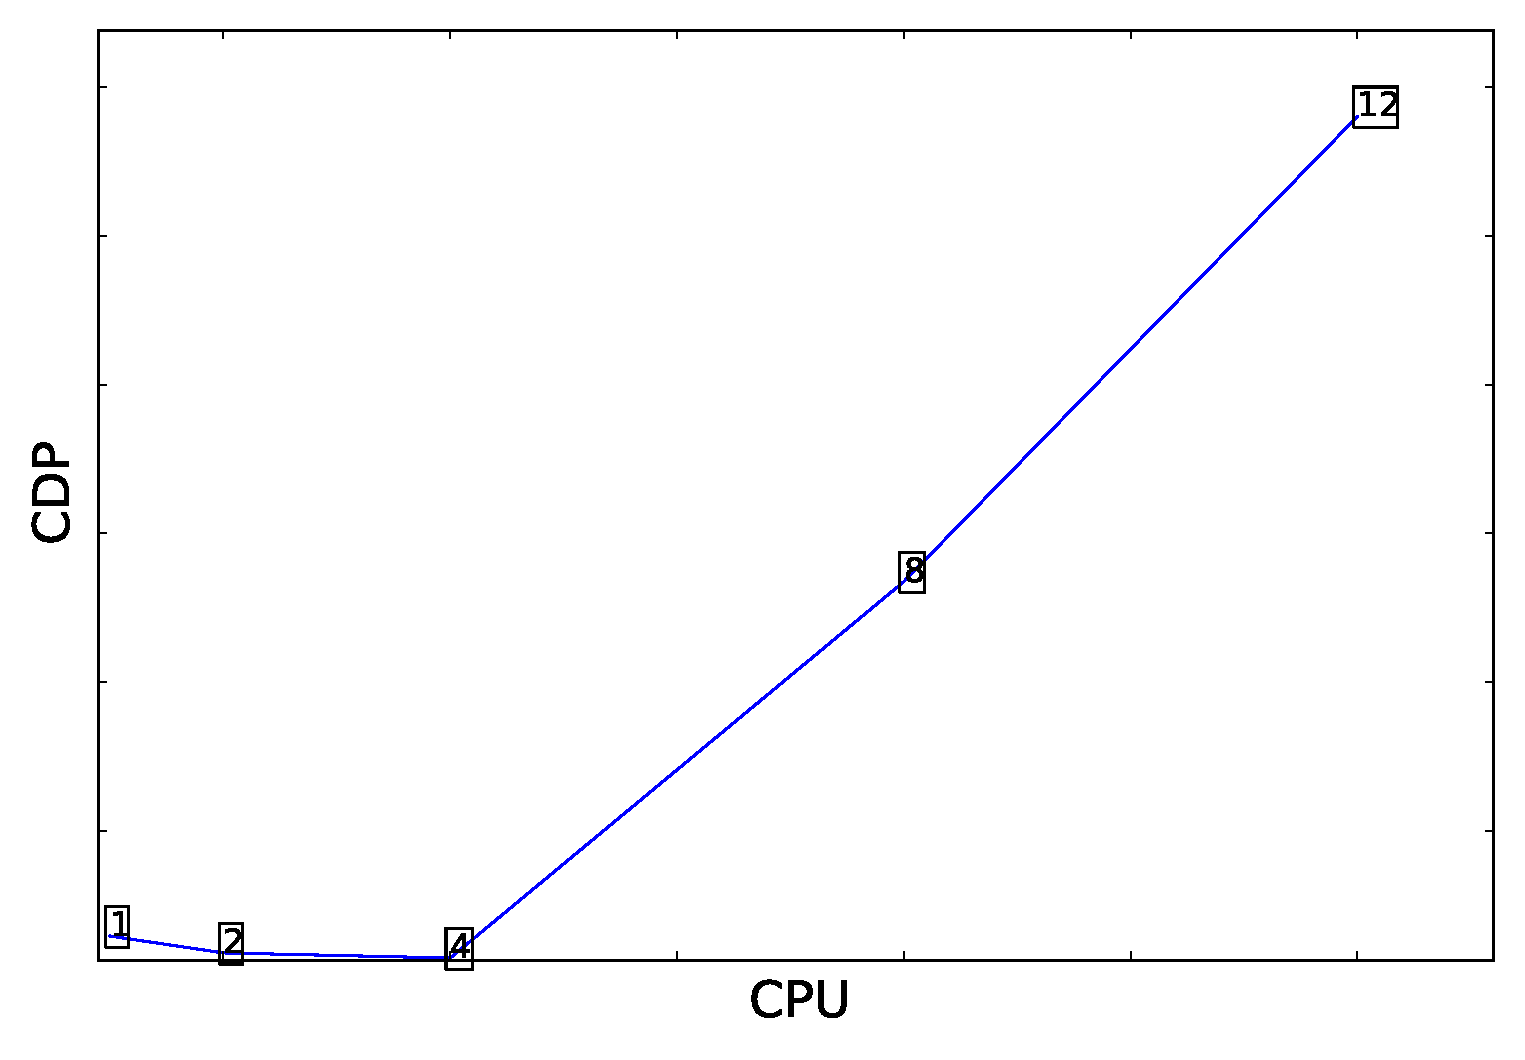
\includegraphics[width=\textwidth]{Chapter-8/figures/regression_cpu_CDP_12_1.eps}
        \caption{Regression}
        \label{fig:regression_cdp}
    \end{subfigure}
    \bigskip
    \begin{subfigure}[b]{0.3\textwidth}
        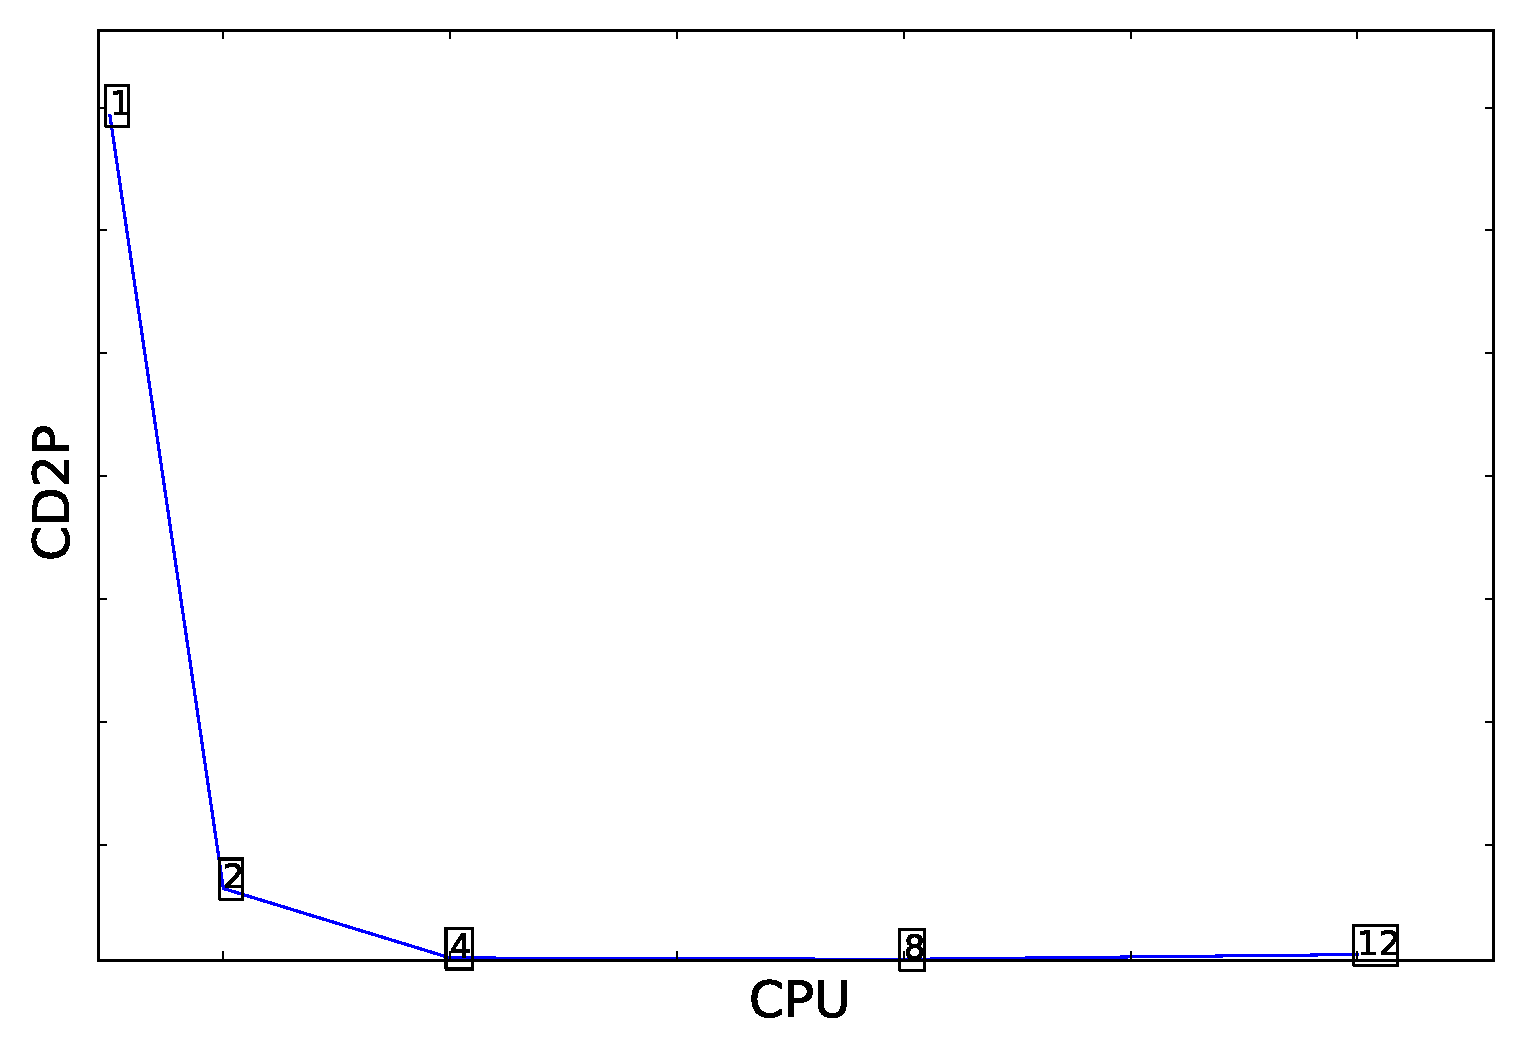
\includegraphics[width=\textwidth]{Chapter-8/figures/pagerank_cpu_CD2P_12_1.eps}
        \caption{PageRank}
        \label{fig:pagerank_cd2p}
    \end{subfigure}
    \begin{subfigure}[b]{0.3\textwidth}
        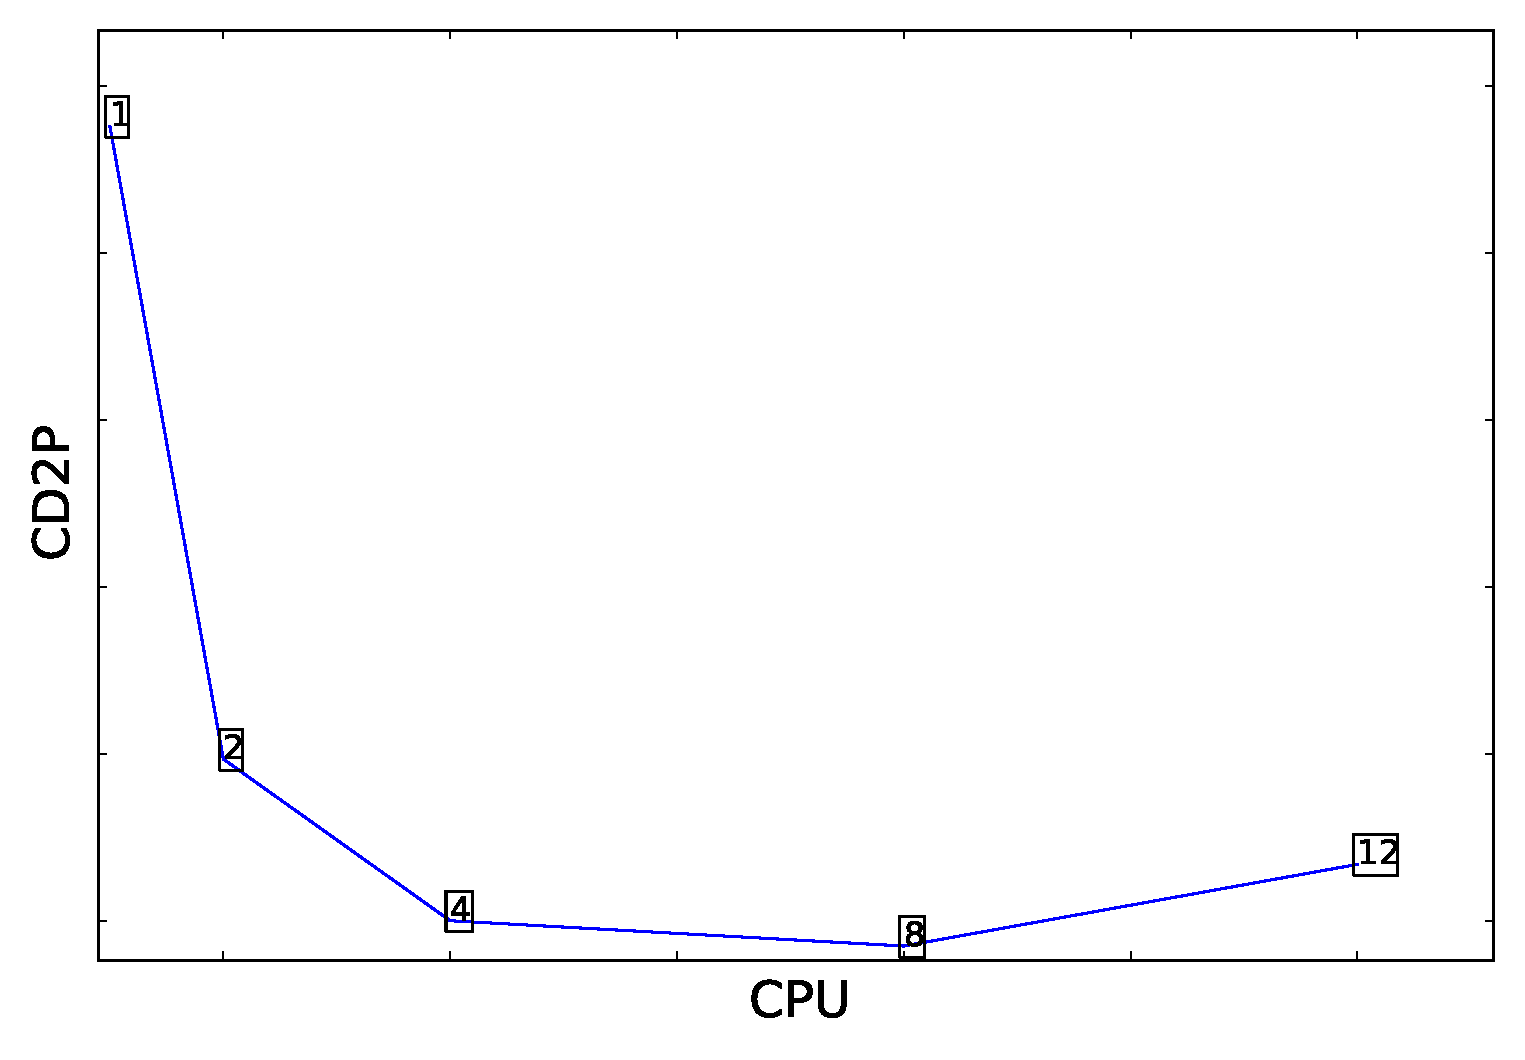
\includegraphics[width=\textwidth]{Chapter-8/figures/webloganalysis_cpu_CD2P_12_1.eps}
        \caption{Web Log Analysis}
        \label{fig:webloganalysis_cd2p}
    \end{subfigure}
    \begin{subfigure}[b]{0.3\textwidth}
        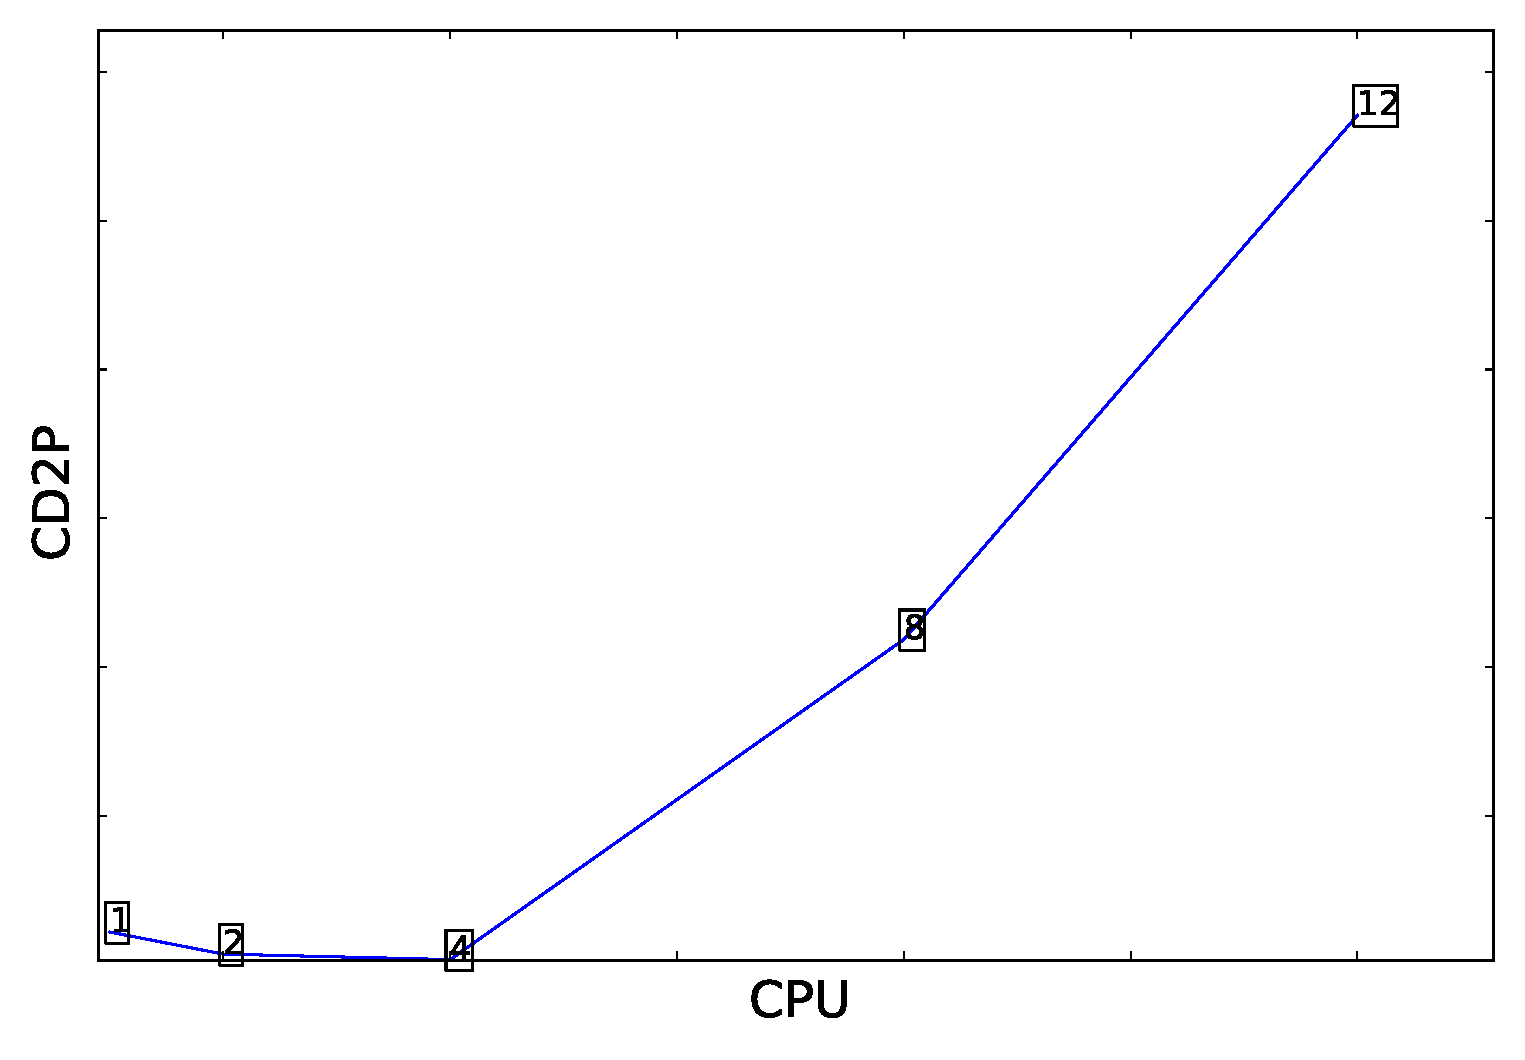
\includegraphics[width=\textwidth]{Chapter-8/figures/regression_cpu_CD2P_12_1.eps}
        \caption{Regression}
        \label{fig:regression_cd2p}
    \end{subfigure}
    \bigskip
    \begin{subfigure}[b]{0.3\textwidth}
        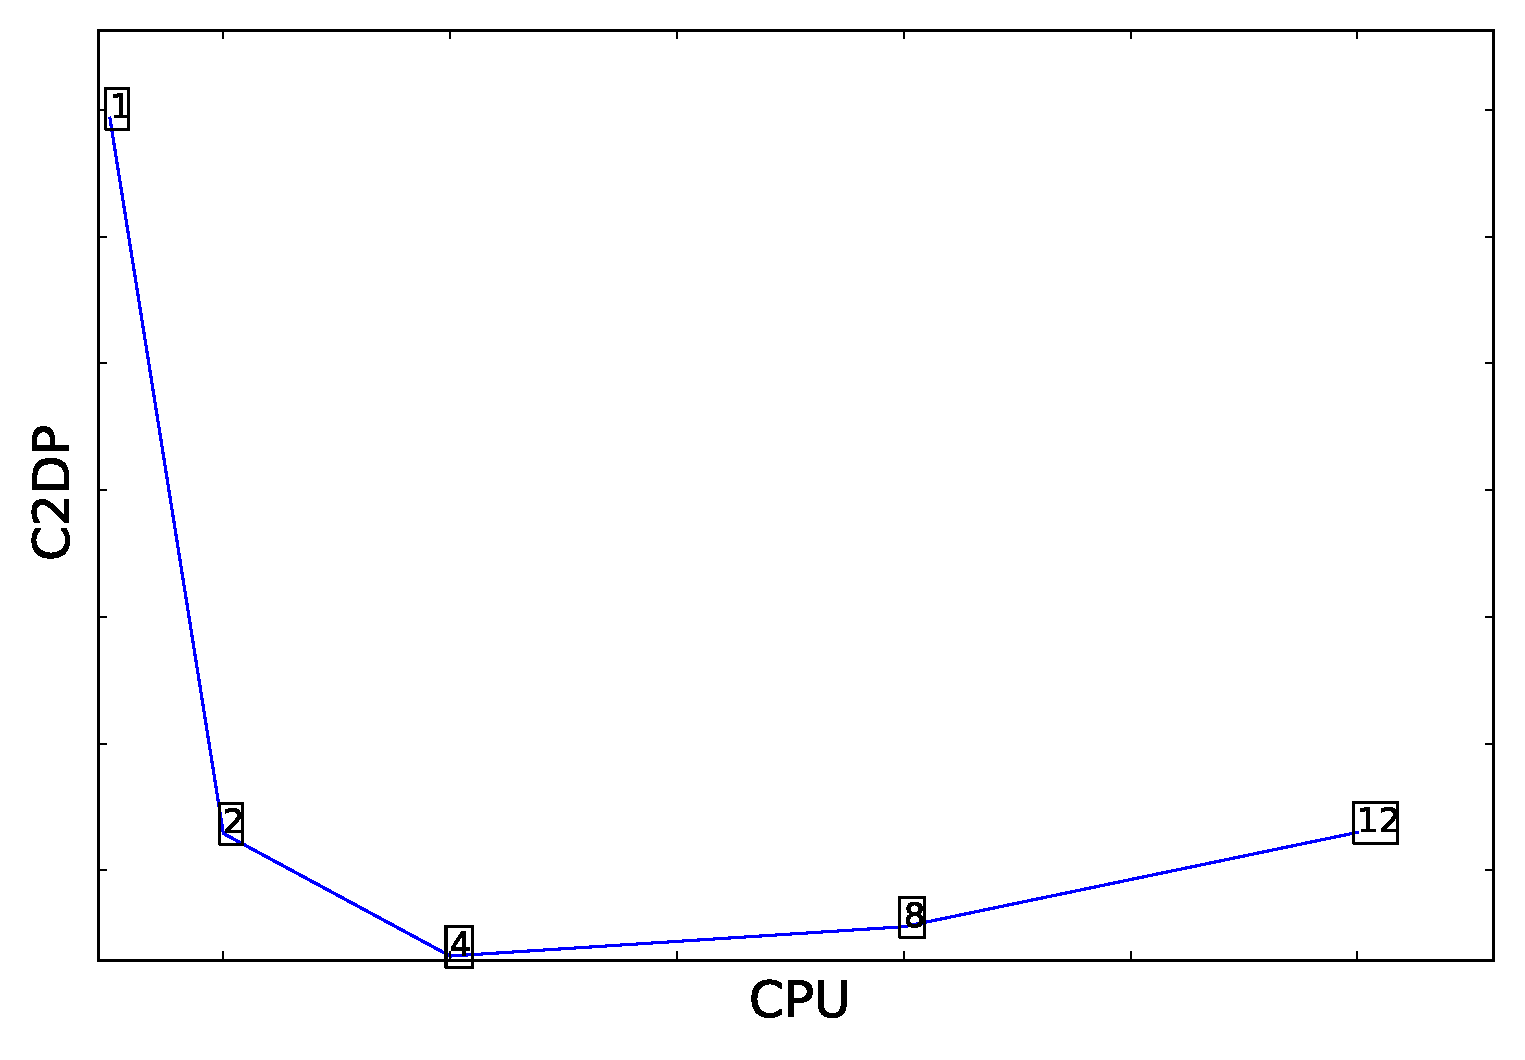
\includegraphics[width=\textwidth]{Chapter-8/figures/pagerank_cpu_C2DP_12_1.eps}
        \caption{PageRank}
        \label{fig:pagerank_c2dp}
    \end{subfigure}
    \begin{subfigure}[b]{0.3\textwidth}
        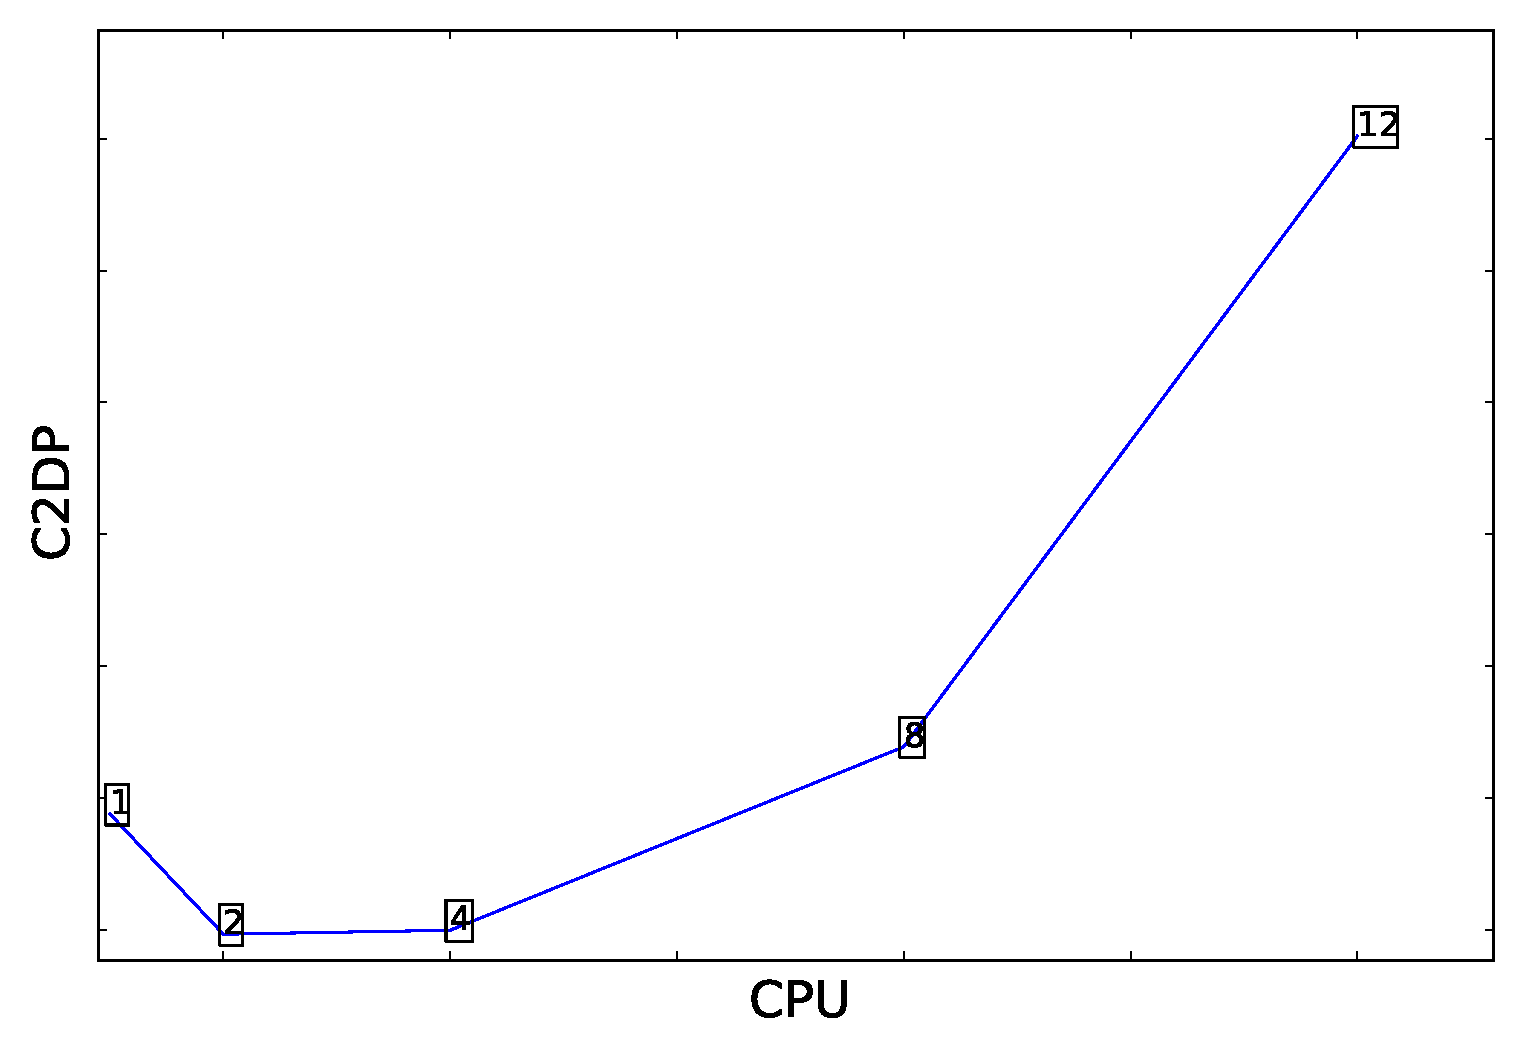
\includegraphics[width=\textwidth]{Chapter-8/figures/webloganalysis_cpu_C2DP_12_1.eps}
        \caption{Web Log Analysis}
        \label{fig:webloganalysis_c2dp}
    \end{subfigure}
    \begin{subfigure}[b]{0.3\textwidth}
        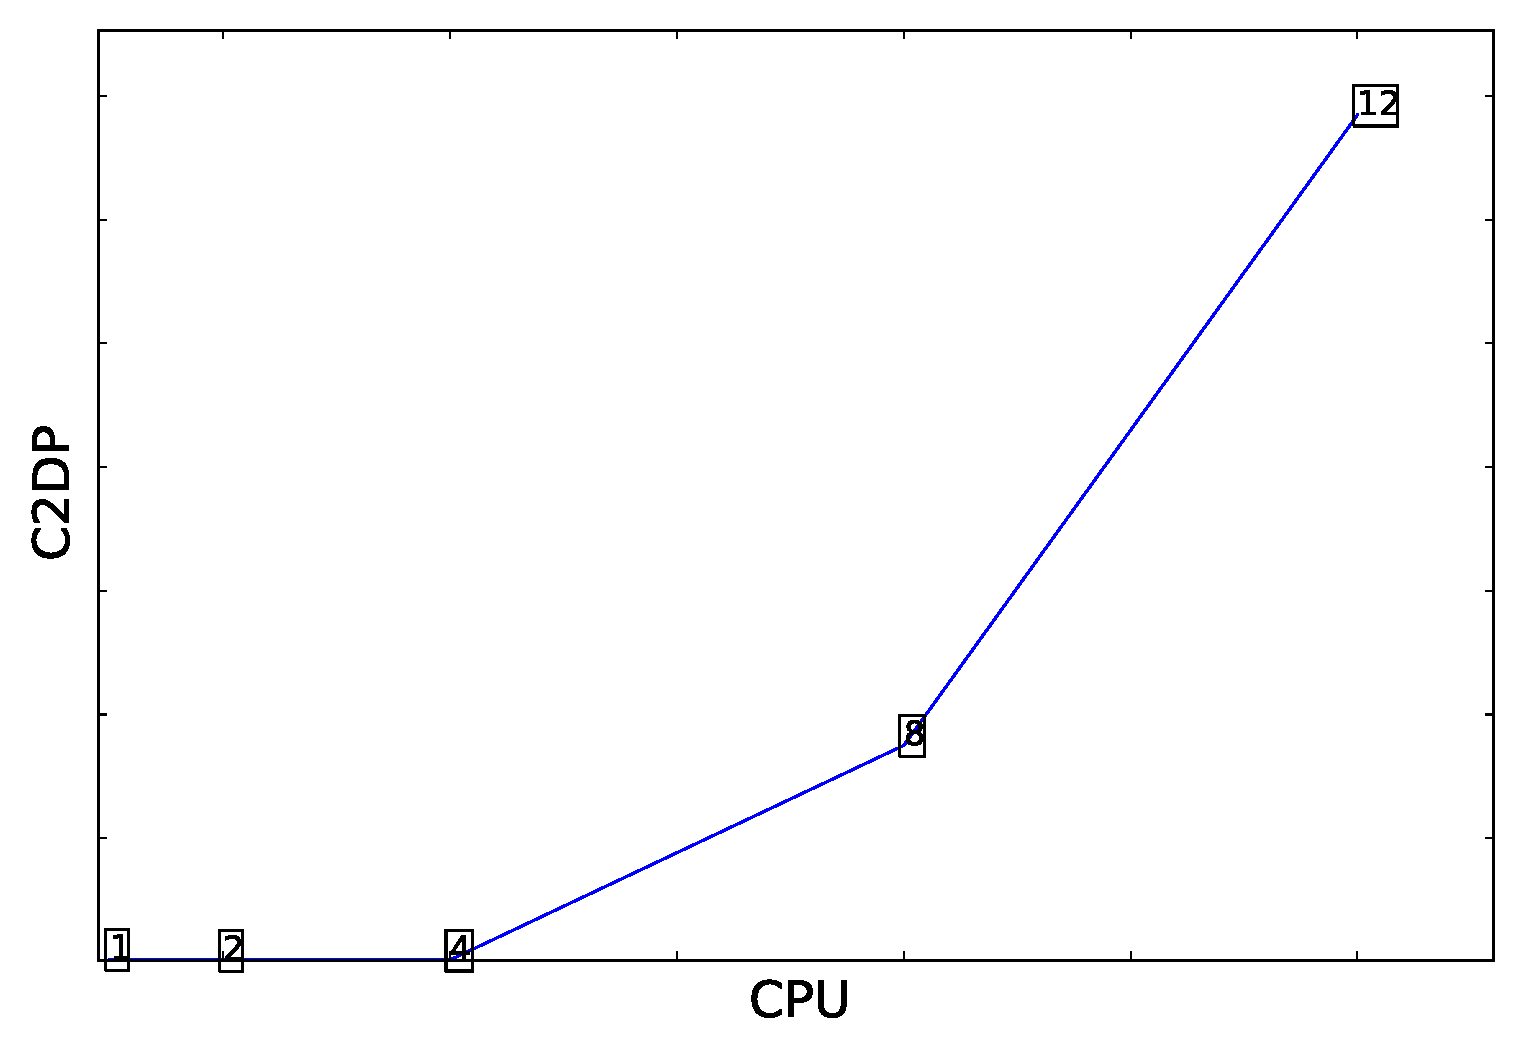
\includegraphics[width=\textwidth]{Chapter-8/figures/regression_cpu_C2DP_12_1.eps}
        \caption{Regression}
        \label{fig:regression_c2dp}
    \end{subfigure}
    \caption{CDP analysis for the cost and time trade-off}
    \label{fig:cdp_analysis}
\end{figure}
\fi



Our preliminary evaluations have shown that
it is not obvious to choose the \emph{best} configuration
because there is no clear relationship between \emph{time} and \emph{cost}.
Besides, applications have very different trade-off curves.
It requires a thorough understanding of application performance and resource capability
for finding out the most cost-effective configurations,
given a time and cost objectives.

\fi


\section{Conclusion}

Cloud architecture tuning is essential for hosting applications in the cloud.
In this chapter, we formulate the CAT problem and
describe its challenges.
We also present the state-of-the-art approaches and discuss
their pros and cons.
In the following chapters,
we will study how to incorporate low-level insights to improve a CAT method.
We will demonstrate how to build a practical system that delivers an effective
CAT solution.

%\section{Objectives}



We also look at other metrics for comparing CAT methods.
First, it is important to deliver \emph{reliable}
search performance and search cost across different workloads.
Some optimizers may encounter the fragility issue because
the search space is hard to model~\cite{Hsu2018Arrow}.
Second, a CAT method must be \emph{scalable}.
\emph{Ernest}, for example, must build a prediction model
for each VM family. 
Last, the optimizer must use a generic approach for adapting to
the rapid changes in cloud computing and software systems.
Exploiting workload information and system internals
can improve prediction performance but
makes a CAT method less applicable to distinct systems
~\cite{Wang2004,Venkataraman2016}.







\chapter{Background and Related Work}
\label{chapter:background}

This chapter describes the necessary background that is related to
the research problems addressed in this dissertation.
We first describe data-intensive computing and its storage architecture.
Next we discuss performance prediction for distributed systems.
Last, we discuss related work that uses the data-driven approach
to optimize system performance.



\chapter{Background and Related Work}
\label{chapter:background}

This chapter describes the necessary background that is related to
the research problems addressed in this dissertation.
We first describe data-intensive computing and its storage architecture.
Next we discuss performance prediction for distributed systems.
Last, we discuss related work that uses the data-driven approach
to optimize system performance.



\chapter{Background and Related Work}
\label{chapter:background}

This chapter describes the necessary background that is related to
the research problems addressed in this dissertation.
We first describe data-intensive computing and its storage architecture.
Next we discuss performance prediction for distributed systems.
Last, we discuss related work that uses the data-driven approach
to optimize system performance.



%\chapter{Background and Related Work}
\label{chapter:background}

This chapter describes the necessary background that is related to
the research problems addressed in this dissertation.
We first describe data-intensive computing and its storage architecture.
Next we discuss performance prediction for distributed systems.
Last, we discuss related work that uses the data-driven approach
to optimize system performance.



\chapter{Workload-Aware Data Placement}
\label{chapter:dp}

A CAT optimizer determines the best architectural choices.
For example, users can scale out or shrink in a cluster size to meet workload changes.
In this chapter, we focus on optimizing performance after a software system
is reconfigured.

% Claims
% 1. Uniform elasticity is suboptimal in many cases
% 2. Workload-aware data placement increases the system performance
%    - coarse-grained: 15% for powerlaw workload distribution (common workload)
% 3. Placement strategy (to show the tradeoff)
%    - increasing color span (rainbow) → better balancing workload
%    - minimizing color span (monochromatic) → largely exploting caching locality
% 4. Hybrid placement strategy shows both advantages

\section{Introduction}
\label{sec:introduction}

In large-scale, distributed systems the dataset, which is too large
for a single node, is partitioned among the nodes.
Incoming workload (\emph{i.e.,} requests) is routed among nodes by a
load balancer.
For extreme horizontal scaling to be effective, it is necessary for
nearly all requests to be routed to a node containing the needed data
locally, which avoids unnecessary node-to-node interactions.
Consequently, data replication and data placement are components of load
balancing and have a substantial impact on system performance.
In the literature, for example,
AUTOPLACER \cite{Rodrigues2013} and MET \cite{Cruz2013}
optimize data placement to fit workload characteristics in NoSQL databases.
Replicating hotter data in storage is a common approach
to balance load \cite{Lim2010}.
In relational databases, sharding is used to distribute load
by partitioning tables to achieve effective horizontal scaling
\cite{Chang2008, george2011hbase, Lakshman2010, Adya2016, Curino2010}.


Cloud computing has changed how computing resources are used.
Before cloud computing, infrastructure is purchased and used for many
years before it is upgraded or replaced.
However, with Infrastructure as a Service (IaaS) equipment is rented
for a short time, including as short as one execution of an
application.
This shift from buying to renting greatly increases the flexibility of
infrastructure available for a given application.
Therefore, rather than tune an application to run well on a specific
machine, a cloud user instead can tune the
infrastructure to accommodate each application on each
dataset.
When an infrastructure is resized in response to changes in workloads,
it is necessary to replicate and place data partitions among nodes.
It is still unclear what are the better strategies
for this decision---prior work on data placement
does not totally address these issues~\cite{Rodrigues2013, Cruz2013, Lim2010}.


Efficient deployment of distributed systems with an
irregular workload requires both cluster sizing and
data placement.
N\"aive uniform data replication (where all data partitions have the
same number of replicas) is effective only when the workload is also
uniform---requests are equally distributed among all partitions.
\emph{Workload-aware} data placement replicates and places
partitions to match the distribution of requests in the anticipated
workload.

\begin{figure}[!htbp]
    \centering
    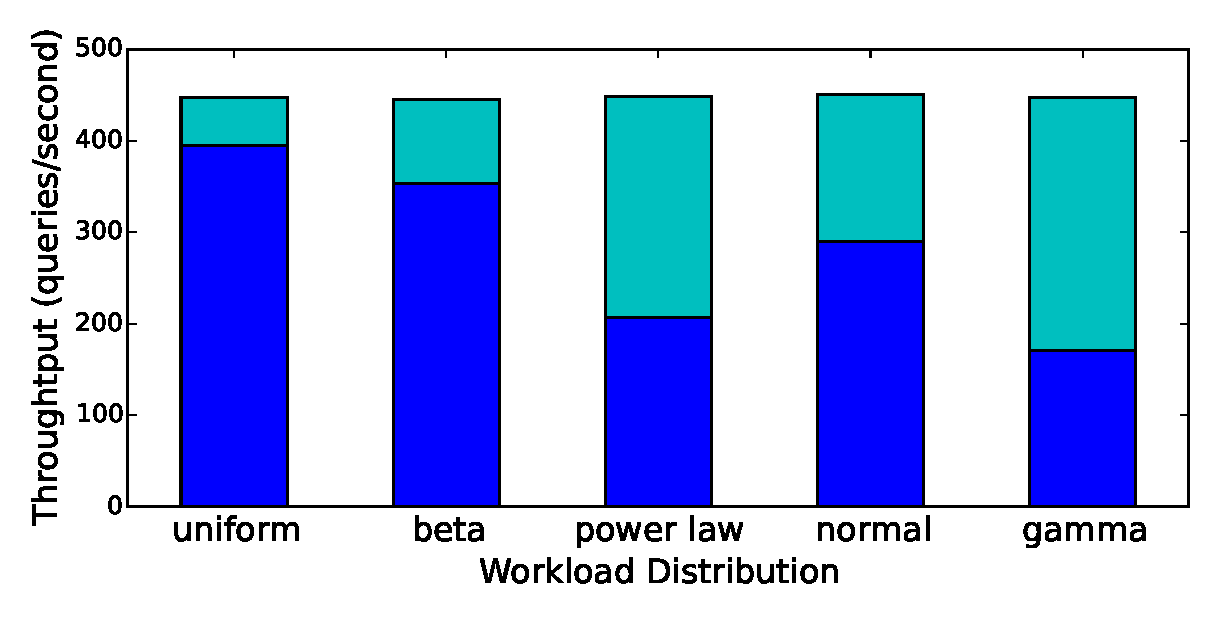
\includegraphics[width=0.8\linewidth]{figures/E34_uniform_suboptimal_tp_stacked_scdm2017.eps}
    \caption{Uniform data placement is suboptimal.
             The lower bar is the measured throughput of uniform placement while
             the upper bar is the performance loss to the idealistic placement.
(Data is a subset of data shown in
\mytable{\ref{tab:throughput_comparison_local}} on Section~\ref{sec:evaluation}.)}
    \label{fig:uniform_suboptimal}
\end{figure}

\myfigure{\ref{fig:uniform_suboptimal}} illustrates the cost of
uniform data replication on non-uniform workloads.
The results for five different workloads are presented on the $x$-axis;
the skew (degree of imbalance) in the workload increases from
left to right.
The \emph{complete} placement solution, where each node has all data,
is an idealistic upper bound on the potential gains of
matching data replication and workload.
% Uniform placement is within 10\% of ideal when the workload is
% uniform.
Because any node can process a request, new requests are sent to the
least loaded node and the performance of \emph{complete} is flat across all
workloads.
In this example, the cluster has twice the minimum capacity, so uniform
replication has two copies of each partition.
Therefore, a request must be sent to
one of the two nodes that hold the data associated
with the request.
Throughput decreases as the
workload skew increases because some nodes are over loaded and
others are under utilized.
While uniform placement achieves 88\% of ideal on uniform workload, it
is only 38\% of ideal on the highly-skewed gamma workload.
This example illustrates the need to properly \emph{replicate} and
\emph{place} data on the nodes of a cluster.


This chapter explores the three dimensions that affect data placement.
The first dimension is \emph{granularity} of data partitions.
Fine-grain (more than one partition per node) placement has costs
(overhead) and benefits (flexibility).
The second dimension is how many \emph{replicas} of each partition.
We let the anticipated demand per partition (\emph{i.e.}, the
\emph{workload}) 
determine the replication factor for each data partition.
The hotter the data, the greater the replication.
The number of data partitions influences how closely the replication
matches the workload.
However,
a coarse-grain partition (one per node) is unlikely to match the
workload.
Last, fine-grain partitioning introduces the
\emph{placement} dimension because there are several ways to distribute
the partitions among the nodes.

We present results from a simulation program that
examines these three dimensions.
We find that coarse-grain placement does not provide sufficient
flexibility to balance non-uniform loads.
A surprisingly small amount of additional partition granularity
is sufficient to load balance and obtain most benefits.
The work presents and evaluates the tradeoff between several
fine-grain placement strategies that either
increase robustness to tolerate workload deviation or
reduce storage footprint.

To further examine these conclusions, our empirical study
on an HPCC cluster\footnote{HPCC Systems is an open source
  \emph{data-analytics computer}---a highly scalable, distributed
  framework for processing and analyzing
  large datasets---supported by LexisNexis Risk Solutions at
  \url{https://hpccsystems.com/}.
}
shows that proper data replication and placement
affect system performance greatly.
The coarse-grain scheme improves system throughput by
$25\%$ and $85\%$ for the normal and power law distribution,
respectively.
A fine-grain placement strategy 
improves query throughput by $52\%$ and $105\%$.
On the most highly-skewed case, the improvement is $166\%$ increase over the
n\"aive solution.

Because data placement relies on a prediction of the upcoming
workload, which will invariably be wrong to some degree.
This chapter, therefore, considers the \emph{robustness}, which
is a measure to describe how sensitive a data placement scheme is to
slightly mis-predicted workloads, of several placement strategies.
Results show that maximizing the number of unique partitions per node
increases the robustness of a placement.
\section{Modeling Data Replication and Placement}
\label{sec:model}

Our work concerns systems in which the dataset
must be partitioned among the nodes because the dataset
is too large to be completely
replicated on each node.
We replicate subsets of the whole dataset in order to increase
throughput and decrease latency.
While replication for availability is critically important, it is not a
subject of this research. 

Distributed, large-scale systems such as
Apache Hadoop, Spark, Cassandra, and Ceph
largely exploit data locality while reducing node-to-node
communication for achieving high horizontal
scaling~\cite{DeanJ2004_MapReduce,zaharia2010spark,Lakshman2010,SageWeil2006Ceph}. 
Data partitions are replicated as the system scales out.
An inefficient data placement scheme is unable to achieve the
optimal system performance and service-level objective (SLO)
violations may occur~\cite{Rodrigues2013,Cruz2013,Trushkowsky2011,Majors2010}.

The goal of this work is to place data partitions onto nodes such
that the performance is maximized for the upcoming workload.
There is a large body of work supporting workload
prediction~\cite{Gmach2007,box2015time,Akdere2012}.
This work assumes that a reliable (though not
necessarily perfect) prediction is provided by some other work.
Instead of solely relying on accurate workload prediction,
systems can dynamically adjust replication factors
and data locations for handling workload changes
~\cite{Lim2010, Trushkowsky2011, Cruz2013}.
This work focuses on determining the optimal
partition granularity, replication factors, and placement strategy.
Our work is complementary to a dynamic approach.

The following model characterizes the 
\emph{data replication and placement problem} in large-scale,
distributed systems. 
Let $M>1$ be the minimum cluster size that is sufficient to hold all
data.
The storage capacity is strictly limited by the amount of data it
physically can store locally.
In many real-world applications, $M$ is in the hundreds of nodes.
However, for this model it is only necessary that $M$ not be equal to
one, which does not require data partitioning.

Let $N$ ($N \ge M$) be the number of nodes in a cluster.
When the workload changes, the cluster expands ($N$ increases)
to meet increased demand and minimize QoS violations, or it contracts
($N$ decreases) to reduce resources and cost. 
But the cluster cannot contract smaller than the $M$ nodes needed to
hold the data.

The data is partitioned into $k \ge 1$ equal-sized data partitions on each node.
Thus, the dataset has $P = Mk$ unique partitions.
Because the cluster has $N$ nodes, there are $S = Nk$ \emph{slots} for
data partitions.
We define the \emph{replication factor}, $R$, as $R=N/M$.
When $R>1$, then $N>M$ and $S > P$ and some partitions will
be replicated among
the ``extra'' slots.
\emph{Coarse-grain} data placement occurs when there is only one
partition per node, $k=1$.
\emph{Fine-grain} data placement, $k>1$, which has more total
data partitions and partition slots, supports more distinct placements
than coarse-grain providing a better opportunity to match the
workload, and increases performance.

\medskip
\begin{tabular}[h]{lll}
  \multicolumn{3}{l}{\textbf{Model parameters}}\\
  ~~~~&\emph{Minimum number of nodes:} & $M>1$\\
  &\emph{Per node granularity:} & $k\ge 1$ \\
  &\emph{Replication factor:} & $R\ge 1$ \\
  \multicolumn{3}{l}{\textbf{Derived terms}}\\
  &\emph{Instantiated nodes:} & $N=RM$\\
  &\emph{Unique data partitions:} & $P = Mk$\\
  &\emph{Slots:} & $S = Nk = RMk$\\
\end{tabular}
\medskip

We present a motivating example below.
The base cluster has four nodes, $M=4$.
The current demand is twice the current capacity.
\myfigure{\ref{fig:dp_before_coarse}}
shows the load per partition on four nodes.
The load is unevenly distributed among the partitions.
In particular, in terms of node capacity the load on the four partitions in
\myfigure{\ref{fig:dp_before_coarse}} is 3.5, 2, 1.5, and 1 (which
conveniently totals 8).
\myfigure{\ref{fig:dp_before_fine}}, shows the same
aggregate demand as it is distributed among 16 partitions, four per
node: $k=4$.
Fine-grain replication gives rise to a \emph{placement} decision.
Redistributing loads helps reduce load imbalance among nodes
by placing highly requested partitions onto least loaded nodes.
In \myfigure{\ref{fig:dp_before_fine_placement}} the load is nearly
balanced: two nodes have a load of 2.125 and two have 1.875.
However, this alone does not help solve the overloading issue
because the workload demand is twice the system capacity.

Suppose the cluster doubles in size to eight nodes exactly meeting
anticipated demand: $R=2$ and $N=8$.
Uniform replication onto eight nodes creates two replicas of each
partition as shown in \myfigure{\ref{fig:dp_uniform}}.
The red box above the two left-most nodes shows the excess demand on those
nodes as 3.5 units of node capacity are serviced by two nodes.
The white regions in the four right-most nodes show the
underutilization because the demand is less than the capacity.

A coarse-grain, non-uniform solution is clearly better
than uniform because \emph{hotter} partitions can be
replicated more than \emph{colder} ones.
For example, in \myfigure{\ref{fig:dp_coarse}} the 3.5 units of P1 are
distributed over three nodes.
Unsurprisingly, a fine-grain solution can better match the demand to
the capacity.
\myfigure{\ref{fig:dp_fine_monochromatic}} shows that demand is perfectly matched to
capacity in this idealized example.


\myfigure{\ref{fig:dp_fine_rainbow}} shows a second placement that also
perfectly balances load but has four unique partitions on each
node.
The nodes in \myfigure{\ref{fig:dp_fine_monochromatic}} have either
one or two unique partitions.
Fewer unique partitions per node reduces the footprint of both primary
(memory) and secondary (disk) storage.
On the other hand,
more unique partitions per node increases the number of nodes that can
respond to a given request, which may better share the load among nodes.

This simple example was constructed to clearly show
the benefits of non-uniform, fine-grain data placement.
Unless the demand is uniformly distributed among the partition (an
extremely unlikely occurrence as explained in
Section~\ref{sec:workloads}) then a n\"aive uniform placement leads to
over- and underutilization.


\begin{figure}[!htbp]
\begin{subfigure}[b]{0.75\textwidth}
    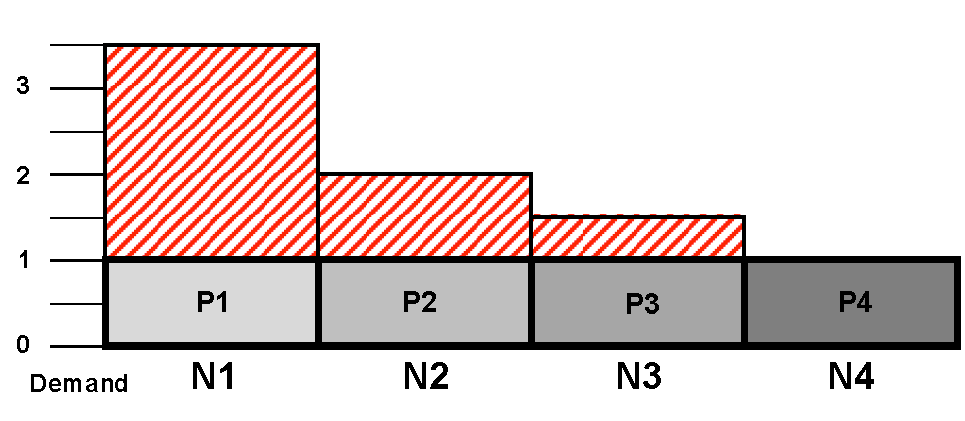
\includegraphics[width=\linewidth]{figures/dp_final_before_coarse.pdf}
    \caption{Coarse-Grain ($M=4,R=1,k=1$)}
    \label{fig:dp_before_coarse}
\end{subfigure}
\begin{subfigure}[b]{0.75\textwidth}
    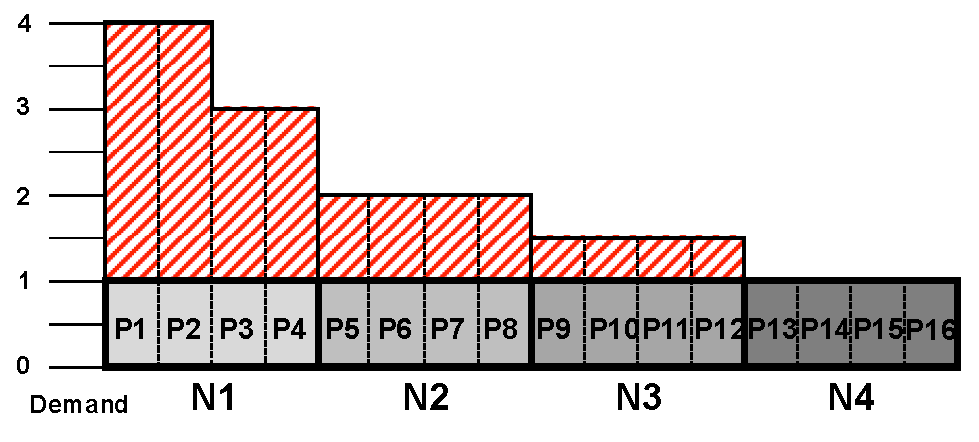
\includegraphics[width=\linewidth]{figures/dp_final_before_fine.pdf}
    \caption{Fine-Grain ($M=4,R=1,k=4$)}
    \label{fig:dp_before_fine}
\end{subfigure}
\begin{subfigure}[b]{0.75\textwidth}
    \includegraphics[width=\linewidth]{figures/dp_final_before_fine_R1.pdf}
    \caption{Fine-Grain alternative placement}
    \label{fig:dp_before_fine_placement}
\end{subfigure}
\centering
\caption{The workload demand exceeds the system capacity.}
\label{fig:dp_before}
\end{figure}


\begin{figure}[!htbp]
\begin{subfigure}[b]{0.9\textwidth}
    \includegraphics[width=\linewidth]{figures/dp_final_uniform.pdf}
    \caption{Uniform data placement ($M=4,R=2,k=1$)}
    \label{fig:dp_uniform}
\end{subfigure}
\hfill
\begin{subfigure}[b]{0.9\textwidth}
    \includegraphics[width=\linewidth]{figures/dp_final_coarse.pdf}
    \caption{Coarse-grain data placement ($M=4,R=2,k=1$)}
    \label{fig:dp_coarse}
\end{subfigure}
\hfill
\begin{subfigure}[b]{0.9\textwidth}
    \includegraphics[width=\linewidth]{figures/dp_final_fine_monochromatic.pdf}
    \caption{Fine-grain \emph{compact} data placement ($M=4,R=2,k=4$)}
    \label{fig:dp_fine_monochromatic}
\end{subfigure}
\hfill
\begin{subfigure}[b]{0.9\textwidth}
    \includegraphics[width=\linewidth]{figures/dp_final_fine_rainbow.pdf}
    \caption{Fine-grain \emph{balanced} data placement ($M=4,R=2,k=4$)}
    \label{fig:dp_fine_rainbow}
\end{subfigure}
\centering
\caption{Different data placement schemes.}
\label{fig:dp_schemes}
\end{figure}

\section{Workloads}
\label{sec:approach}

This section presents the data placement problem.
First, it characterizes the workloads used in the work.
Next, it expounds on the three dimensions of the problem:
(1) granularity, (2) replication, and (3) placement.
Last, it explains and analyzes three data placement methods,
comparing
performance in terms of load imbalance, storage footprint, and robustness.

\subsection{Workload Characteristics}
\label{sec:workloads}

A workload can be described with several critical characteristics,
such as arrival rate and autocorrelation.
Because this work considers data replication and placement, 
the workload characteristic that matters most is access frequency of the
individual elements of the
dataset, such as, the pages of a web server or the keys in an index.
Other characteristics are not factored into
this work because they do not have a direct impact on data replication
or placement.

A uniform workload is atypical and likely artificial,
which is unsurprising because
non-uniform workloads are common in many natural settings
~\cite{Pavlo2012}.
For example, the normal (Gaussian) distribution can be observed
in class score distribution,
while the log-normal distribution is useful to describe
the response file size in web servers~\cite{Barford1998}.
In addition, the power law probability distribution is widely applicable to
web hits, word frequency, personal income, \emph{etc}.\ and tends to
be highly skewed towards a small subset of the full
dataset~\cite{Newman2005}.
That is, a small number of partitions accounts the vast majority of key access
and most of the partitions are touched infrequently. 
Several studies show that frequency of access to different pages or
keys often follows a Zipf or power law distribution.
This has been shown in web servers~\cite{dilley1998web,panteleenko2003web},
video streaming~\cite{sripanidkulchai2004analysis}, 
and Wikipedia traffic~\cite{urdaneta2009wikipedia} to name a few.

In this work, we consider the
\emph{normal} and the \emph{power law} distribution for their
wide appearance in many workloads.
We also consider the \emph{uniform} distribution for a n\"aive baseline,
\emph{beta}, which is less skewed than
\emph{normal} and \emph{power law}, and
\emph{gamma}, which generates the highest skewed workload and
has been used in modeling workloads in storage systems~\cite{Wilkes2001}.


\mytable{\ref{tab:load-imbalance}} shows
the five workload distributions used in the work.
This table presents the distribution of the
requests on each of four partitions ($M=4$, $k=1$).
There are 30,000 unique requests among the 1024 keys,
and the average is 7,500 requests per partition.
The requests-per-node values are ordered in decreasing magnitude.
As expected there are approximately the same number of requests for
each partition in the uniform distribution.
The \emph{max:mean} column shows the ratio of the maximum number of requests
to the average.
Because the total running time is largely dependent on the slowest or
most heavily loaded node, the max-mean ratio foretells the performance
penalty for each workload on a uniform distribution.
The ratio for uniform is 1.01, meaning the maximum is 1\% greater
than the average.
But the highly-skewed gamma distribution has one partition that receives
no requests and one has more than three times the average.
It is clear from \mytable{\ref{tab:load-imbalance}} that in
non-uniform workloads
the maximally loaded partition demands
more resources than the other partitions.
The final column presents access imbalance using the 
\emph{skew} metric~\cite{Pavlo2012}. 

This work evaluates the problem using synthetic workloads.
An alternative is to evaluate using real-world traces.
But such traces are in short supply.
Moreover, a trace represents a very specific situation that may not be
representative of a general class.
Additionally, a trace has many characteristics that are hard to
control.
Using synthetic workloads enables us to evaluate more distributions and
confine the observed effects to the change in distribution.


\begin{figure}[!htbp]
\begin{subfigure}[b]{0.45\textwidth}
    \includegraphics[width=\linewidth]{figures/E45_simulation_imbalance_coarse_std_uniform.eps}
    \caption{uniform}
\end{subfigure}
\begin{subfigure}[b]{0.45\textwidth}
    \includegraphics[width=\linewidth]{figures/E45_simulation_imbalance_coarse_std_beta.eps}
    \caption{beta}
\end{subfigure}
\begin{subfigure}[b]{0.45\textwidth}
    \includegraphics[width=\linewidth]{figures/E45_simulation_imbalance_coarse_std_powerlaw.eps}
    \caption{power law}
\end{subfigure}
\begin{subfigure}[b]{0.45\textwidth}
    \includegraphics[width=\linewidth]{figures/E45_simulation_imbalance_coarse_std_normal.eps}
    \caption{normal}
\end{subfigure}
\begin{subfigure}[b]{0.45\textwidth}
    \includegraphics[width=\linewidth]{figures/E45_simulation_imbalance_coarse_std_gamma.eps}
    \caption{gamma}
\end{subfigure}
\centering
\caption{The load distribution among nodes under the coarse-grain data placement ($M=64, k=1$).}
\label{fig:simulation_imbalance_coarse}
\end{figure}


\begin{figure}[!htbp]
\begin{subfigure}[b]{0.45\textwidth}
    \includegraphics[width=\linewidth]{figures/E45_simulation_imbalance_fine_std_uniform.eps}
    \caption{uniform}
\end{subfigure}
\begin{subfigure}[b]{0.45\textwidth}
    \includegraphics[width=\linewidth]{figures/E45_simulation_imbalance_fine_std_beta.eps}
    \caption{beta}
\end{subfigure}
\begin{subfigure}[b]{0.45\textwidth}
    \includegraphics[width=\linewidth]{figures/E45_simulation_imbalance_fine_std_powerlaw.eps}
    \caption{power law}
\end{subfigure}
\begin{subfigure}[b]{0.45\textwidth}
    \includegraphics[width=\linewidth]{figures/E45_simulation_imbalance_fine_std_normal.eps}
    \caption{normal}
\end{subfigure}
\begin{subfigure}[b]{0.45\textwidth}
    \includegraphics[width=\linewidth]{figures/E45_simulation_imbalance_fine_std_gamma.eps}
    \caption{gamma}
\end{subfigure}
\centering
\caption{The load distribution among nodes under the fine-grain data placement with various $k$ ($M=64, R=2$).}
\label{fig:simulation_imbalance_fine}
\end{figure}


\begin{table}[!htbp]
  \centering
  \caption{Load-imbalance of workloads.}
  \resizebox{\columnwidth}{!}{%
  \begin{tabular}[h]{lrrrrcc}
    \toprule
Distribution & 	\multicolumn{4}{l}{Requests for individual partitions}
    & max:mean & skew\\
\midrule
Uniform & \textbf{7,565} & 7,548 & 7,449 & 7,438 & 1.01 & 0.15\\
Beta & \textbf{10,313} & 10,288 & 4,715 & 4,684 & 1.38 & 0.39\\
Power law & \textbf{17,344} & 8,795 & 3,361 & 500 & 2.31 & 0.60 \\
Normal & \textbf{14,882} & 14,827 & 149 & 142 & 1.98 & 0.74\\
Gamma & \textbf{23,542} & 6,329 & 129 & 0 & 3.14 & 0.77\\
\bottomrule
  \end{tabular}
  }
  \label{tab:load-imbalance}
\end{table}


%%%%%%%%%%%%%%%%%%%%%%%%%%%%%%%%%%%%%%%%
% Approaches
%%%%%%%%%%%%%%%%%%%%%%%%%%%%%%%%%%%%%%%%

\subsection{Data Placement Steps}
\label{sec:dp_methods}

A data placement method requires determining
partition granularity, replication factors, and placement schemes.
Partition granularity represents the smallest unit
for replicating data and calculating loads.
The coarsest granularity is one partition per node ($k=1$), and
the finest is one partition per key.
A small $k$ decreases the likelihood of balancing a non-uniform workload.
However, a large $k$ increases management overhead.

Once the partition granularity $k$ is determined,
the next step
in deriving a solution is determining the number of
replicas for each partition based on the expected workload.
For example, suppose there are four partitions ($P=4$) with a
replication factor of four ($R=4$), then
there are sixteen slots for these partitions ($S=16$) in a
coarse-grain solution.
Given a uniform expected workload the replication factor vector would be 
[4, 4, 4, 4], that is there are four copies of each of the four
partitions. 
For a workload with a normal distribution the replication factor
vector might be [2, 6, 6, 2] and for 
power law it might be [1, 2, 4, 9].
In general, there is no perfect match between the vector and the
anticipated workload.

Assuming that the predicted load on each partition is $\lambda_i$ and the total
load is $\Lambda = \sum_{i=1,P}\lambda_i$.
The replication problem is to determine the \emph{replication vector},
$\vec{R}, R_i \in \mathcal{I}$, such that
$R_i \ge 1~\forall i$  and
$S = \sum_{i=1,P}R_i$.
In words, the replication vector contains the number of replicas (an
integer value) of each partition, such that the total number of
replicas equals the number of slots available.
The replication error is
$E = \sum_{i=1,P} | R_i/S - \lambda_i/\Lambda |$, which is the
accumulation of difference between 
the actual relative
replication of each partition ($R_i/S$) and
the anticipated relative
workload per partition ($\lambda_i/\Lambda$).

%\input{tables/delta_powerlaw}

The last step is assigning the replicas to the slots on the nodes.
For coarse-grain, the number of replicas equals the number of
slots and there is only one possible placement.
But for fine-grain, $k>1$, there are many possible placements.
One placement strategy is to minimize the number of unique
partitions on each node in order to reduce dataset footprint on the
nodes.
We call this strategy \emph{compact}.
If there are multiple choices,
it picks the node with the least load.
The opposite strategy to \emph{compact} is \emph{full},
which maximizes the number of different partitions on each node and
also picks the node with the least load.
The third strategy is placing partitions in order to balance loads as much as possible.
We call this strategy \emph{balanced}. 
We show that although \emph{full} and \emph{balanced} have
different goals, the resultant placements and effects are similar.
Furthermore, \emph{compact} and \emph{full}
balance loads among the
nodes with their best efforts within their given constraints.
Consequently, all three strategies achieve good load balancing, of
course \emph{balanced} is a slightly better at it.
To reiterate:
The goal of \emph{compact} is reducing the number of unique partitions
on each node, which reduces the 
footprint of the data set.
On the other hand, the goal of \emph{full} is to distribute
replicas for the same partition to as many nodes as possible---balancing
the load---with the intent of increasing the availability of hot partitions. 



Our data placement procedure is described in Algorithm \ref{alg:dp}.
This is a framework and therefore, different placement strategies can be used.
The complexity for generating the replication vector is proportional
to the number of partitions, $\mathcal{O}(Mk)$.
Different placement strategies implement distinct
\emph{pick\_node} functions,
which is $\mathcal{O}(N)$.
This function is executed for each slot ($Nk$).
Therefore, the total complexity is of the placement algorithm
is $\mathcal{O}(kN^2)$.
Although it is quadratic, it is in the number of nodes that, even in a
very large cluster, is tractable.
A straightforward Python implementation executes in under few seconds
when $N=256$ and $k=16$.
Furthermore, this solution is a heuristic, it does not find the
optimal solution.
However, the solution is nearly optimal and because it is based on a
prediction of anticipated load optimal is unnecessary.


\begin{algorithm}[!htbp]
 \SetAlgoLined
 \DontPrintSemicolon
 \DontPrintSemicolon
 \KwIn{an historical workload}
 \KwOut{partition placement on each node}
 $M$ := the minimum number of nodes that hold all data\;
 $k$ := the selected partition granularity\;
 $R$ := the replication factor\;
 $loads$ := the predicted loads $\lambda_i$ of partitions\;
 $replicas$ := the replication vector (see Section~\ref{sec:model})

 \For{$p_i$ in $replicas$}{
   \For{$j$=1; $j<=p_i$; $j=j+1$}{
   	 /* strategy is \emph{compact}, \emph{balanced} or \emph{full} */\;
     n := pick\_node(strategy)\;
     assign $p_i$ to $n$
   }
 }
 \caption{Data Placement Procedure}
 \label{alg:dp}
\end{algorithm}




\subsection{Tradeoffs in Placement Strategy}
\label{sec:dp_tradeoff}

Our data placement framework is shown in Algorithm~\ref{alg:dp}.
This framework yields several variants of data placement
when choosing different placement strategies.
This section compares their effects on load balancing and storage footprint.

\subsubsection{Load Balancing}
The primary goal of data placement is distributing workloads evenly among nodes.
A highly skewed system is more likely to encounter performance bottlenecks.
Therefore, a well-balanced system achieves a higher system throughput.
To explore the benefit of fine-grain replication and placement, we
evaluate the effectiveness of 
our data placement schemes in balancing the anticipated workload.
We generated 100 instances of workloads, of 300,000 queries, for each of
the five distributions.
The workload instances vary because the access counts are generated
probabilistically.
Each generated workload is considered a prediction of the upcoming
workload.

First, we evaluate how the replication factor $R$ affects load balancing.
This simulation is conducted with $M=64$ and $k=1$.
We use the box plot, as shown in \myfigure{\ref{fig:simulation_imbalance_coarse}},
to analyze the loads distributed among nodes.
The bottom and top of the rectangle represent the first and third quartile of loads.
The red line is the median, and the red dot is the mean.
To facilitate comparison, the loads are normalized so that the means equal one.
Above the box is the whisker that is calculated by
adding $1.5$ times the interquartile range (IRQ) to the third quartile.
Similarly, the whisker below the box is the first quartile
minus $1.5$ times the IRQ.
The plus signs represent the data points that have the loads
beyond the two whiskers.
These is the standard representation for a box plot.
In a well balanced system, the median and mean values
will be close and the box will be small.

This figure clearly shows that increasing the replication factor
reduces load imbalance to a degree.
However, this alone is insufficient to eliminate
under-utilized loads totally because
increasing the number of replicas only reduces the loads.
The only way to reduce under utilization is
to overlap under and over utilized partitions,
which is not possible in the coarse grain method. 
Therefore, the replication factor alone is not sufficient
for balancing loads because it does not reduce under-utilization.
Take the \emph{gamma} distribution for example,
when $R=1$, most of the nodes are under utilized (low median) and
few nodes have extremely excess loads (large size box).
Doubling the replication factor creates more overloaded nodes
because $R=2$ is not enough to distribute loads.
As $R$ increases, the median value moves closer to the mean and
the variance (the size of box) also decreases,
which suggests over-utilization is mostly addressed.
However, increasing $R$ is still insufficient because
there are still many outliers (beyond the two whiskers).


Next, we examine how much the partition granularity can reduce load imbalance.
We run a set of simulations with $M=64$, $R=2$, and various $k$ values,
and choose \emph{balanced} as the placement scheme.
\myfigure{\ref{fig:simulation_imbalance_fine}} clearly shows that
fine partition granularity greatly reduces load imbalance.
Even in the most skewed workload (gamma), $k=16$ is able to almost perfectly balance loads.
For most workloads, $k=4$ is sufficient to reduce the load imbalance
below $10\%$.
When workloads are highly skewed (the \emph{normal} and \emph{gamma} case),
their load imbalance (the size of box in the figure) drops greatly from $k=1$ to $k=2$
because finer partitioning provides higher flexibility to mix
over- and under-utilized partitions on the same node.
Increasing partition granularity eventually leads to (for all
practical purposes)
perfectly balanced loads.


\begin{figure}[!htbp]
    \centering
    \includegraphics[width=0.8\textwidth]{figures/E42_simulation_colors_resized_powerlaw.eps}
    \caption{The number of unique partitions per node (storage footprint) under different placement schemes.}
    \label{fig:simulation_colors}
\end{figure}

\subsubsection{Storage Footprint}
There are $S=Nk$ choices for placing a partition replica.
When placing multiple replicas of the same partition on the same node,
it reduces the number of unique partitions per node.
When the number of unique partitions per node is lower,
it generally requires lower storage footprint.
A lower storage footprint reduces memory pressure, and may lead to higher cache efficiency.
We run a set of simulations with $M=64$, $R=2$ and various $k$.
This work only presents the results of the \emph{power law} workloads.
Other workload cases show very similar effects.

\myfigure{\ref{fig:simulation_colors}} shows the average number of
unique partitions on each node.
By definition all partitions in 
\emph{full} are unique and it is always 1 (normalized).
\emph{Balanced} is very nearly 1 in all cases.
On the other hand, as $k$ increases, 
\emph{compact} tends to $0.5$, which is $1/R$.
We further investigate how the replication factor affects storage footprint.
\myfigure{\ref{fig:simulation_colors_replication}} shows that the
number of unique partitions tends to $1/R$ as $k$ increases,
which is the desired outcome of the \emph{compact} scheme.


\begin{figure}[!htbp]
    \centering
    \includegraphics[width=0.8\textwidth]{figures/E42_simulation_colors_replication_resized_powerlaw.eps}
    \caption{The number of unique partitions per node under the \emph{compact} method with various $k$.  The number converges at $k=32$, which is equal to $1/R$.}
    \label{fig:simulation_colors_replication}
\end{figure}

\section{Evaluation}
\label{sec:evaluation}

This section presents our evaluation.
We introduce our experimental setup and benchmark
design.
We then evaluate different placement schemes
by measuring query throughput and
testing their robustness to slight workload mispredictions.


\subsection{Experiment Setup}

We conducted our evaluation on Virtual Computing Lab (VCL), a cloud
platform provided by NC State University.
All servers are equipped with 2-core Intel Xeon CPU and 8GB memory
and connected to a 10 Gbit switch. 
VCL only provides limited storage capacity of local disks or
\emph{instance storage}.
This is also the case for many cloud configurations.
In fact, a majority of EC2 instance types in Amazon Web Services (AWS) do not
have any instance storage.
Instead one must mount a remote volume served by a enterprise-level
storage system.
(AWS calls this \emph{elastic block storage}--EBS.)
We evaluate our approach using both instance storage (local disks) and
remote volumes provided by network file system (NFS),
backed by NetApp 2554 filer with dual controllers.

We evaluate our placement schemes on
high performance computing cluster (HPCC)~\cite{middleton2011hpcc}.
HPCC is an open source
data analytics computer developed by LexisNexis Risk
Solutions for processing big data.
They maintain several clusters with more than 100 nodes, the largest
with more than 500, to provide services to their clients.
Experiments were conducted on a HPCC Roxie cluster.
Roxie is a \emph{data delivery engine} that responds to queries.
It finds the answers to requests in an index that is partitioned and,
if desired, replicated across the nodes.
Roxie is optimized to handle massive amounts of concurrent requests
with low latency.

Data replication and placement that fit workload demands
have direct performance impact on performance.
Roxie clusters partition and distribute data
with two replicas per partition by default.
We modified Roxie to incorporate our data placement schemes.
Our approaches are not specific to Roxie.
They should be able to apply to
Apache Hadoop, HBase, Cassandra, and Ceph, providing benefit when
workloads are not uniformly distributed across
keys, partitions or nodes.


\subsection{Workload Generator and Benchmark Suite}

To evaluate the results learned in our simulation, we developed a
distributed benchmark tool 
that is able to issue a large volume of concurrent queries to
Roxie. 
This benchmark tool adopts the master-slave architecture, where
the the master node generates workload according to a workload profile, and
the slave nodes execute the query requests.
This tool is customizable and supports any number of
workload distributions.
This benchmark suite is written in Python, and designed for testing
query performance at large scale.

In our evaluation, we are interested in how placement schemes
with different levels of partition granularity
respond to different types of workload distribution.
We consider \emph{uniform}, \emph{beta}, \emph{power law}, \emph{normal}, and \emph{gamma} distributions.
The beta distribution is defined on the interval $[0, 1]$ with
two shape parameters, $\alpha$ and $\beta$.
We choose $\alpha=2$ and $\beta=2$ for the base case of beta distribution. 
The power law distribution is controlled by the
\emph{shape} parameter and we choose $3$ for the base case.
Regarding the normal (or Gaussian) distribution it has a
\emph{mean} and a \emph{standard deviation} parameter, which is
$0$ and $1$ in our case.
The gamma distribution also has a \emph{shape} parameter and the base case
uses $5$.
%\ick[redundant?] -> we didn't specify the parameters in detail.
A single instance of each workload is used in all the empirical tests
of Roxie so that results can be compared across multiple runs and
different configurations.
The specific workloads used are those shown in
\mytable{\ref{tab:load-imbalance}}.


\subsection{Benchmark Steps}

To best measure the performance, our benchmark service runs
one worker node for each Roxie server, which 
eliminates the performance impact at the client side.
We use separate machines from the Roxie cluster on the VCL for the benchmark service.
The Roxie controller node dispatches requests and synchronizes with workers.
Worker nodes request jobs and execute them as soon as possible.


We generate the five workload distributions
with different access counts to keys.
All datasets are 128GB.
Next, we specify the smallest cluster size $M$,
the replication factor $R$ (which determines
the cluster size $N$), and
the partition granularity $k$.
In our evaluation, $M$ is equal to 4.
The coarse-grain schemes replicate data on
a node basis.
Fine-grain schemes, on the other hand,
divides the data on a node into 32 equal-size partitions
(1GB per partition).

We compare five placement schemes in total.
First, \emph{base} represents the uniform data placement.
It is coarse grain ($k=1$) and not workload aware.
The \emph{coarse} scheme is also coarse-grain but replicates partitions
based on anticipated workload.
For the fine-grain schemes ($k=32$), we consider
\emph{compact} to reduce storage footprint while maximizing cache locality,
and \emph{balanced} to minimize load imbalance among machines.
In our evaluation, we found that the \emph{balanced} and \emph{full} scheme
have comparable performance.
Due to the page limit, we report the results of \emph{balanced} in most cases.
Last, the \emph{complete} is an ``idealistic'' placement where each
node holds the entire dataset.
It represents an upper bound.

\begin{table}[t]
\centering
\caption{Steady-State Throughput Comparison (instance storage)}
\resizebox{\columnwidth}{!}{%
\begin{tabular}{llllll}
\toprule
{} &  Uniform & Beta &  Power Law & Normal  &   Gamma \\
\midrule
\emph{base}          & 394.8            &  353.5            &  206.6             &    290.4             &  171.2 \\
\emph{coarse}        & -                &  367.8 ($4.0\%$)  &  381.9 ($84.9\%$)  &    364.0 ($25.3\%$)  &  309.7 ($80.9\%$) \\
\emph{compact}       & 375.4 ($-4.9\%$) &  377.5 ($6.8\%$)  &  383.2 ($85.5\%$)  &    374.6 ($29.0\%$)  &  374.2 ($118.6\%$) \\
%Rainbow       & 388.6 ($-1.6\%$) &  398.8 ($12.8\%$) &  438.7 ($51.1\%$)  &    416.8 ($101.8\%$) &  438.5 ($156.2\%$) \\
\emph{balanced}      & 408.1 ($3.4\%$)  &  412.6 ($16.7\%$) &  422.8 ($104.7\%$) &    442.5 ($52.4\%$)  &  455.9 ($166.3\%$) \\
%MCMLB         & 447.0 ($6.8\%$) &  449.0 ($14.8\%$) &  484.0 ($56.1\%$)  &    460.0 ($119.4\%$) &  483.0 ($201.9\%$) \\
\emph{complete}      & 446.8 ($13.2\%$) &  445.4 ($26.0\%$) &  448.3 ($117.0\%$) &    450.1 ($55.0\%$)  &  447.0 ($161.1\%$) \\
\bottomrule
\multicolumn{6}{r}{unit: queries/second} 
\end{tabular}
}
\label{tab:throughput_comparison_local}
\end{table}


Our next step is to change the data layout in Roxie to reflect
the desired data placement decision.
The Roxie cluster is restarted to load the new data layout.
To avoid cache interference, the file system cache is cleared
before every benchmark run.

Last, a workload profile is submitted to the benchmark controller.
The controller node generates the query plan accordingly.
In this way, the same stream of requests is presented for each
benchmark, which allows us to verify results with multiple identical
runs and to compare results from different placements.
We collect query throughput during the entire benchmark process.

\subsection{Steady-State Throughput}
\label{sec:throughput}

We conduct this evaluation to test steady-state throughput.
We generate 30,000 requests for each of the five workload
distributions.
We then calculate the average throughput over the sampling period
(the first and last $10\%$ period are not included.)
This measurement ensures we capture the stable throughput, but not
the warm-up period (low throughput) and
the long-tail period (system is not saturated).


\begin{figure}[!htbp]
\begin{subfigure}[b]{0.6\textwidth}
    \includegraphics[width=\linewidth]{figures/E38_robustness_std_beta.eps}
    \caption{Beta}
    \label{fig:robustness_beta}
\end{subfigure}
\begin{subfigure}[b]{0.6\textwidth}
    \includegraphics[width=\linewidth]{figures/E38_robustness_std_powerlaw.eps}
    \caption{Power Law}
    \label{fig:robustness_powerlaw}
\end{subfigure}
\begin{subfigure}[b]{0.6\textwidth}
    \includegraphics[width=\linewidth]{figures/E38_robustness_std_gamma.eps}
    \caption{Gamma}
    \label{fig:robustness_gamma}
\end{subfigure}
    \centering
    \caption{Compare robustness under slight workload mispredictions. The $y$-axis represents queries per second, and starts from 200 for better presentation to tell performance difference.}
    \label{fig:robustness}
\end{figure}


\subsubsection{Local Storage}

Our evaluation starts with storing data required for Roxie queries
on local disks.
This evaluation involves 8 Roxie nodes: $M=4$ and $R=2$.
\mytable{\ref{tab:throughput_comparison_local}} shows the throughput
of proposed replication and placement schemes under
different workloads.
The values in parenthesis are the speedup relative to \emph{base} performance at
the top of each column.
The \emph{base} placement strategy is uniform.
It does not perform well as
the skewness of workload increases.
For example, the power law workload in the uniform data placement
can only achieve $52.3\%$ of the throughput of a uniform workload.
The second strategy is also coarse grain but replicates according to
anticipated workload.
On a uniform workload this is the same as \emph{base}.
It out performs \emph{base} on skewed workloads.
For example, it
achieves $84.9\%$ more throughput than \emph{base} on \emph{power law}.


Two fine-grain approaches, \emph{compact} and \emph{balanced}, which
further improve performance over \emph{coarse}, are also shown.
In the normal workload case, \emph{compact} and \emph{balanced}
improve on \emph{coarse} by an additional $10.6$ and $78.5$ queries per second.
In the gamma case, \emph{balance} adds $146.2$ queries,
a $47.2\%$ improvement over \emph{coarse}.
Workload-aware data placement is preferable for non-uniform workloads.
The fine-grain strategies out perform \emph{coarse} on all the skewed
workloads.
This is attributed to better load balancing.
As skew increases, the benefit from fine-grain increases (because the
load imbalance in \emph{coarse} increases).


\begin{comment}
\begin{table*}[h]
\centering
\caption{Steady-State Throughput Comparison}
\begin{tabular}{llllll}
\toprule
{} &  Uniform & Beta &  Normal &  Power Law &   Gamma \\
\midrule
Base          & 399.0           &  267.0          &  227.0           &    180.0           &  159.0 \\
Coase         & -               &  368.0 ($38\%$) &  362.0 ($59\%$)  &    371.5 ($106\%$) &  309.5 ($\ \ 95\%$) \\
Monochromatic & 402.5 ($0.9\%$) &  409.0 ($53\%$) &  410.0 ($81\%$)  &    403.5 ($124\%$) &  399.0 ($151\%$) \\
Rainbow       & 426.0 ($6.8\%$) &  431.0 ($61\%$) &  405.5 ($79\%$)  &    442.0 ($146\%$) &  427.0 ($169\%$) \\
Complete      & 438.0 ($9.8\%$) &  414.0 ($55\%$) &  433.0 ($91\%$)  &    449.0 ($149\%$) &  431.0 ($171\%$) \\
\bottomrule
\multicolumn{6}{r}{unit: queries/second} 
\end{tabular}
\label{tab:throughput_comparison}
\end{table*}
\end{comment}


\begin{table}[t]
\centering
\caption{Steady-State Throughput Comparison (NFS)}
\resizebox{\columnwidth}{!}{%
\begin{tabular}{llllll}
\toprule
{} &  Uniform & Beta &  Power Law &  Normal &   Gamma \\
\midrule
\emph{base}       & 446.1            &  383.1            &  220.2             &    393.3             &  176.4 \\
\emph{coarse}     & -                &  396.4 ($3.5\%$)  &  415.3 ($88.6\%$)  &    379.6 ($29.4\%$)  &  327.9 ($85.9\%$) \\
\emph{compact}    & 403.7 ($-9.5\%$) &  416.2 ($8.7\%$)  &  401.3 ($82.3\%$)  &    407.1 ($38.8\%$)  &  407.8 ($131.1\%$) \\
%Rainbow   & 447.3 ($0.3\%$)  &  428.1 ($11.8\%$) &  474.0 ($61.6\%$)  &    469.0 ($113.0\%$) &  481.5 ($172.9\%$) \\
\emph{balanced}   & 447.6 ($0.3\%$)  &  440.8 ($15.1\%$) &  454.0 ($106.2\%$) &    469.7 ($60.1\%$)  &  485.9 ($175.5\%$) \\
%MCMLB     & 447.9 ($0.4\%$)  &  448.8 ($17.2\%$) &  479.8 ($63.6\%$)  &    455.5 ($106.9\%$) &  482.0 ($173.2\%$) \\
\emph{complete}   & 484.2 ($9.0\%$)  &  485.6 ($26.8\%$) &  492.4 ($123.7\%$) &    495.0 ($68.8\%$)  &  490.0 ($177.8\%$) \\
\bottomrule
\multicolumn{6}{r}{unit: queries/second} 
\end{tabular}
}
\label{tab:throughput_comparison_nfs}
\end{table}


The \emph{complete} solution out performs all others, including both fine-grain
solutions.
This is because while the workload was probabilistically generated
over 30,000 requests.
The workload for each small window of requests does not always reflect
the overall workload.
In such cases, \emph{complete} performs better.
However, \emph{complete} is generally not feasible
when dataset is too large to fit into one node.

Overall, workload-aware data placement significantly increases query throughput.
Using fine partition granularity better balances the load.
\emph{Balanced} performs better than \emph{compact}, indicating that
the benefit of a smaller footprint is less than the cost of poorer load
balancing.
The \emph{balanced} scheme is occasionally competitive with \emph{complete}.

\subsubsection{Remote Storage}
Next, we evaluate our proposed schemes against data storing on remote storage.
The Roxie cluster size and the number of benchmark clients remain the same
with the local storage case.
\mytable{\ref{tab:throughput_comparison_nfs}} details the throughput numbers.
This evaluation confirms the general observations seen in the instance
storage test.
However, the throughput is higher using remote storage.
While somewhat counter intuitive, it is not unheard.
This occurs because local storage uses plain commodity disks and the
% not sure the original sentence is grammerly correct
filer uses high-performance disks as well as aggressive caching.
Moreover, the I/O demand does not exceed the capacity of the NFS server.
Therefore, the additional network traffic is not creating a
performance bottleneck.


\subsection{Robustness Comparison}
\label{sec:robustness}

We are interested in how sensitive a placement scheme is to minor
deviations in the anticipated workload.
(Tables~\ref{tab:throughput_comparison_local} and
\ref{tab:throughput_comparison_nfs} show performance degradation for
major deviations.)
We say a placement scheme is more \emph{robust} when the scheme works
well even when the actual workload is slightly different from the
anticipated workload.
We pick different parameters for generating slight workload variance.
For example, we change the shape parameter in the power law distribution.
Therefore, it becomes either less or more skewed.
We create two less and two more skewed workloads for each type.

\myfigure{\ref{fig:robustness}} shows how different placement schemes react
to workload shifts.
The figure shows the average throughput and the standard deviation
 of the placement schemes under the four ``shifted'' workloads
The figure indicates that the coarse-grain scheme
under performs in both average (lower) and deviation (greater)
compared to the fine-grain schemes.

The \emph{compact} scheme is better than \emph{coarse} but its performance is not as
good as the \emph{balanced} scheme.
The \emph{balanced} scheme overall exhibits higher throughput than
\emph{coarse} and \emph{compact}.
More importantly, \emph{balanced} shows consistent standard deviation
in three workloads.
The highest performance degradations in each workload are
$2\%$, $6\%$ and $3\%$
while the \emph{compact} scheme shows
$3\%$, $5\%$ and $14\%$ (increasing as skewness increases) degradation respectively.
% The \emph{balanced} shows $6\%$ performance loss at most.
% balanced
%  - beta: 436.41 vs 444.75
%  - power law: 442.22 vs. 471.82
%  - gamma: 472.98 vs. 487.88
% compact
%  - beta: 396.85 vs. 410.53
%  - power: 388.71 vs. 408.26
%  - gamma: 350.19 vs. 408.02
The above suggests than \emph{balanced} is more robust then
\emph{compact}, which is robust than \emph{coarse}.
There is little difference between \emph{balanced} and \emph{full} in either
average throughput or standard deviation.
This is because there is little difference in the placement of
partitions---that is, the balanced scheme tends to have a high degree of
unique partitions on each node.



\subsection{Micro Benchmark}

We have presented the steady-state throughput in Section~\ref{sec:throughput}.
In this section, we further examine why different placement schemes
lead to large performance difference.

We investigate resource utilization of different placement schemes
for understanding the tradeoff between the \emph{compact} and
\emph{balanced} scheme. 
We collect system statistics
(\textit{dstat}~\cite{dstat} and \textit{cachestat}~\cite{cachestat})
during the entire benchmark runs.
\mytable{\ref{tab:micro_nfs}} presents the system statistics, and
metrics are normalized to the smallest value in each metric group,
except the \emph{max:mean} ratio. 
This normalization better shows the difference between placement schemes.
Except \emph{mean \%CPU}, a system is more efficient when
the metrics listed are small.
These metrics are collected from the benchmark runs under the gamma workload.
Other workloads present very similar trends.

First, we examine CPU utilization across all Roxie nodes.
The average CPU utilization indicates whether Roxie is fully saturated,
and the \emph{max:mean} metric tells whether loads are well balanced
among Roxie nodes.
In the \emph{base} scheme, CPU utilization is the lowest and load imbalance
is the highest, which explains why uniform data placement under performs.
Workload-aware replication eliminates load imbalance while
improving CPU utilization.
Fine-grain partition further reduces load imbalance,
as in the \emph{balanced} scheme.

\begin{table}[ht]
\centering
\caption{Normalized System Statistics of Roxie Servers}
\resizebox{\columnwidth}{!}{%
\begin{tabular}{lllllll}
\toprule
	& Metrics	&	\emph{base}	&	\emph{coarse} & \emph{compact} & \emph{balanced} & \emph{complete} \\
\midrule
\multirow{2}{*}{Load Balancing} & \% CPU (mean)		& \textbf{1.00} (13\%) & 2.29   & 2.37 & 3.11 & 2.97     \\
		                        & \% CPU (max:mean) & 2.01 & 1.34   & 1.23 & 1.1    & 1.14     \\
\midrule
\multirow{3}{*}{Cache Locality} & cache misses (sum)     & 1.13 & 1.24   & \textbf{1.00} (659K) & 1.26 & 1.22     \\
		                        & dirty pages (sum)     & 1.20 & 1.47   & \textbf{1.00} (200K) & 1.52 & 1.29     \\
		                        & cache sizes (max) & 2.11 & 1.51   & \textbf{1.00} (825MB)   & 1.17 & 1.15     \\
\midrule
\multirow{2}{*}{Efficiency}     & I/O wait (mean) & 1.39 & 6.73   & \textbf{1.00} (2.35\%) & 2.48 & 2.55     \\
		                        & TCP connections (mean)   & 2.40 & 1.53   & 1.31 & 1.10 & \textbf{1.00} (1357) \\
%		                        & disk read         & 2.72 & 2.00   & 1.09 & \textbf{1.00} & 3.48    \\
\bottomrule
\end{tabular}
}
\label{tab:micro_nfs}
\end{table}



Second, we examine the benefits of packing multiple replicas into the same node,
as in the \emph{compact} scheme.
\mytable{\ref{tab:micro_nfs}} shows that cache misses and dirty pages
are significantly lower in the \emph{compact} scheme.
Besides, \emph{compact} has much lower cache sizes, $17\%$ lower than
\emph{balanced} and $51\%$ less than the \emph{coarse} scheme.
Although the \emph{compact} scheme outperforms others in cache locality and
requires less cache,
it does not generate the highest query throughput.
A possible explanation is that requests do not greatly benefit from better cache locality.
We suspect the \emph{compact} scheme is useful especially when query applications
require costly read operations.
% We will need to further investigate this case.

Third, we compare I/O wait time and the number of TCP connections
for comparing their efficiency.
A lower I/O wait time indicates that systems do not waste much time on slow I/O operations.
The \emph{compact} scheme, with maximum cache locality, has the lowest I/O wait value.
The number of TCP connections at a given time is related to processing efficiency.
We observe that the \emph{balanced} scheme yields a lower number of TCP connections
than the other schemes, suggesting that requests complete more quickly.


\subsection{Summary}
Our evaluation provides empirical data to support our findings
in the simulation.
First, workload-aware data placement, both the coarse and fine grain methods,
reduces load imbalance, thereby improving system throughput.
However, the coarse-grain approach is insufficient
when workload is highly skewed.
Finer partitioning further balances the loads and in many cases,
the \emph{balanced} scheme has comparable performance to \emph{complete}
(an ``idealistic'' placement).
Furthermore, both \emph{balanced} and \emph{full} are robust while
\emph{compact} reduces storage footprint to $1/R$. 



%% 
\section{Related Work}
\label{sec:related}

The data replication and placement issues have been extensively studied
in several research domains
including memory cache~\cite{Leff1993,Zaman2011},
distibuted storage systems~\cite{Lim2010},
NoSQL database~\cite{Rodrigues2013,Cruz2013,Corbett2013}
traditional retaional databases~\cite{Pavlo2012,Curino2010},
content delivery network (CDN)~\cite{Laoutaris2006}, etc.

Data replication is a common technique to increase
system performance and availability.
Many distributed systems use multiple replicas to
increase reliability and availability as well as improve system
performance~\cite{hbase,SageWeil2006Ceph}.
This chapter focuses on data replication and
its impact on system performance.
Data placement, on the other hand, determines the locations of data.
Apache Hadoop, for example, writes a replica locally and
two replicas in another rack to improve
system performance~\cite{Xie2010,Eltabakh2011}.
Our work makes contributions in three ways.
First, partition granularity determines the basic unit to calculate load.
Second, data replication is governed by anticipated workload.
Last, data placement chooses the slots on servers for maximizing
load balancing or exploiting cache locality.

Ceph is a distributed storage system
that supports configurable replication factors
for the placement group~\cite{SageWeil2006Ceph}.
Similarily, Apache Hadoop~\cite{hadoop} accepts separate replication factors
for different data chunks.
Optimizing the number of replications per object or data chunk
is a challenging task.
AptStore proposes the Popularity Prediction Algorithm (PPA) by
analyzing file system logs and adjusts replication factors accordingly
for files on Apache Hadoop~\cite{Krish2013}.
Scarlett combines offline log analysis and online prediction to
accurately estimate block popularity~\cite{Ananthanarayanan2011}.
Results show that replicating hotter data avoids bottlenecks,
thereby improving the performance of MapReduce jobs.
% These works greatly improve distributed storage performance but
% do not totally answer all the essential properties of
% data replication and placement.

The NoSQL database is a popular repository for large-scale data
because of they support extreme horizontal
scaling~\cite{Lakshman2010,Chang2008,hbase,mongodb}.
%\cmt{add more citations, eg, hbase, reddis,dynamodb, mongodb.}
Studies have shown that non-uniform query key
causes performance issues.
AUTOPLACER \cite{Rodrigues2013} optimizes the placement
for the top-k objects in the distributed key-value store.
To minimize the maintenance cost of large number of objects,
AUTOPLACER proposes the probabilistic data structure (PAA)
to reduce routing latency.
MET \cite{Cruz2013} is an elasticity framework that 
optimizes data placement to fit workload characteristics for HBase.
It is able to reconfigure HBase dynamically when an HBase cluster
requires expansion or contraction.
MET found that heterogeneous machines can easily lead to load imbalance.
To balance the load on each server, MET groups data partitions
according to their access pattern.
MET models the cost of placing data partitions on nodes, and
uses Longest Processing Time (LPT) to minimize the cost,
which maximizing load sharing among nodes.
%\cmt{what is makespan?}
The above implements a system that replicates and places data according to
data access pattern.
Our work explores how data replication and placement schemes
affect system performance under different workload distribution.

%%%%%%%%%%%%%%%%%%%%%%%%%%%%%%%%%%%%%%%%%%%%%%%%%%%%%%%
% moved fig this from model.tex to make it float to first page of mode
%%%%%%%%%%%%%%%%%%%%%%

%%%%%%%%%%%%%%%%%%%%%%%%%%%%%%%%%%%%%%%%%%%%%%%%%%%%%%%

Elastic storage dynamically expands or contracts a storage cluster.
The elastic controller is responsible for
provisioning resources and adjusting data replication and placement
for efficient storage configurations.
The SCADS director \cite{Trushkowsky2011} is an elastic controller
that automatically scales out a storage system to meet stringent
performance requirements. 
SCADS adopts a model-based approach to correlate request workload and
latency. 
It keeps track of the hottest bins (groups of data), and
dynamically moves these bins to different servers for balancing the load.
SCADS also creates performance models to predict workload and server capacity
for better estimating query latency.
Lim et al. propose a design of elastic storage\cite{Lim2010}.
Scaling a storage system poses challenges such as actuator delays,
measurement accuracy and interference with applications.
Their work puts emphasis on the elastic controller, whereas
we discover the relationship between
workload characteristics and data placement
when scaling a data-intensive application.

Sharding is a common technique to distribute load by
partitioning data across distributed server nodes.
More specifically, sharding is an approach that partitions data
according to keys, where partitions are placed
on different servers independently~\cite{Cattell2011}.
This horizontal scaling enables a distributed system to scale efficiently.
NoSQL databases, such as BigTable~\cite{Chang2008}, HBase~\cite{hbase}
and Cassandra~\cite{Lakshman2010}, rely on sharding
to efficiently balance load.

For relational databases, sharding is heavily used to support
a large volume of queries.
Schism uses graph-partitioning algorithms
to determine the optimal partitioning
for minimizing the cost of distributed transactions~\cite{Curino2010}.
The proposed fine-grained data partition minimizes
the required number of distributed transactions for database applications.
Pavlo \emph{et al}. develop a database tool that is able to generate
optimal database designs for parallel OLTP systems~\cite{Pavlo2012}.
They propose a new search algorithm for partitioning database and
create a cost model to minimize the coordination cost
while maximizing load balance.
Spanner is a semirelational database that
manages replicated data globally and performs resharding
at runtime for better load balancing~\cite{Corbett2013}.
Slicer is an auto-sharding service designed by Google~\cite{Adya2016}.
To leverage Slicer, users are required to
associate incoming requests with a key.
Slicer dynamically maps the key to a proper task
for maximizing load balance.
The above studies implement either
a sharding mechanism or design s generic sharding service,
while our work focuses on understanding the tradeoff
between different data placement schemes
when data partitions required proper placement to
meet workload distribution.

\section{Conclusion}
\label{sec:conclusion}

Efficient deployment of large-scale, distributed systems with
an irregular workload requires both cluster sizing and data placement.
We show the uniform distribution is (unsurprisingly) poor for
typical, non-uniform workloads.
This work further shows that coarse-grain replication can reduce
over-utilization but is unable to address under-utilization.
Finer partition granularity reduces both under- and
over-utilization.
With fine-grain partitioning there is a placement decision.
Maximizing the number of unique partitions per node increases robustness
to workload misprediction,
while minimizing the number reduces storage
footprint.
Our empirical study using an HPCC Roxie cluster shows
the benefit of footprint reduction does not offset cost due to poorer
load balancing.
However, we do not believe this is universally true.

This work focuses on the dimension and tradeoffs of various data
replication and placement strategies.
For our future work, we plan to implement an elastic controller
that incorporates our proposed data placement schemes.
In an elastic system, the gains of the optimal placement must be
offset by the cost of data movement.
Calculating this data movement cost remains as a future work.

\chapter{Conclusions and Future Work}
\label{chapter:conclusion}

\section{Thesis Revisited}
Modern software systems come with a lot of configuration options, which can be tweaked to modify the functional or
non-functional (e.g., throughput or runtime) requirements. Finding
the good or optimal configuration to run a particular workload is essential
since there is a significant difference between the best and the
worst configurations. Many researchers report that modern software
systems come with a daunting number of configuration options~\cite{xu2015hey}.
The size of the configuration space increases exponentially with the
number of configuration options. The long runtimes or cost required
to run benchmarks make this problem more challenging.

Prior work in this area used a machine learning method
to model the configuration space accurately. The model is built sequentially,
where new configurations are sampled randomly, and the
quality or accuracy of the model is measured using a holdout set. This strategy
makes these methods unsuitable in a practical setting since they can be very expensive. On the other hand, there are software systems for which an accurate model cannot be
built.

In this thesis, we introduced techniques and method, which can find good configurations while minimizing the search cost. The central insight of this thesis is: to build a machine learning model (not accurate) which
can differentiate between the good and not so good solutions. 

The important lessons, we learned during the preparation of the thesis are:
\begin{itemize}
    \item \textbf{Clustering: } Early attempts managed to use random sampling along with machine learning models to build accurate models, which can then be used to find good configurations. However, random sampling and accurate machine learning models can lead to an expensive model building process. We attempt to \textbf{reduce the cost of the model building by adding the idea of stratified sampling instead of random sampling} i.e.; we try to cluster the configuration space using a top-down clustering and sampling from each sub-population. We have found stratified sampling can significantly reduce the cost of model building and also reduce the variance in the model built. \\
    \noindent\textbf{Lessons Learned: } Even though we found the stratified sampling approach of \what works for the software systems explored in our paper~\cite{nair2017faster}. However, while performing external validation (with a more diverse set of software systems), we found that \what is not efficient (as shown by our preliminary study). Upon further investigation, we found that we make an important assumption: ``our clustering algorithm (WHERE in our case) returns meaningful cluster''. This assumption meant that we know the distance function applicable to the configuration space, i.e., configurations with shorter distance is similar to the configurations with a larger distance. The ineffectiveness of \what is primarily because our assumption did not hold for the newer configuration spaces.
    
    \item \textbf{Ranking: } A retrospective look on the prior work including our work, made us realize that researchers have been tackling the problem of finding good configuration by transforming the problem to a building accurate model problem. However, the fundamental idea in this work is to use ranking as an approach for building models. The ranking is a useful paradigm to solve the software configuration optimization because (1) ranking is the ultimate goal, (2) Ranking is extremely robust since it is only mildly affected by errors or outliers, and (3) Ranking reduces the number of training samples required to train a model.\\
    \noindent\textbf{Lessons Learned:} The model is built sequentially, where new configurations are sampled randomly, and the quality or accuracy of the model is measured using a holdout set. The size of the holdout set in some cases could be up to 20\% of the configuration space and need to be evaluated (i.e., measured) before even the machine learning model is entirely built. This strategy makes these methods unsuitable in a practical setting since the generated holdout set can be (very) expensive. 
    
    \item \textbf{Sequential Model-based Optimization:}  The problem of finding the (near) optimal configuration is expensive and often infeasible using the current techniques. A useful strategy could be to build a machine learning model which can differentiate between the good and not so good solutions. \flash, a Sequential Model-based Optimization (SMBO), is a useful strategy to find extremes of an unknown objective. \flash is efficient because of its ability to incorporate prior belief as already measured solutions (or configurations), to help direct further sampling. Here, the prior represents the already known areas of the search (or performance optimization) problem. The prior can be used to estimate the rest of the points (or unevaluated configurations). Once one (or many) points are evaluated based on the prior, the posterior can be defined. The posterior captures the updated belief in the objective function. This step is performed by using a machine learning model, also called \textit{surrogate model}. The concept of \flash can be simply stated as:
    \begin{itemize}
        \item Given what one knows about the problem,
        \item what can be done next?
    \end{itemize}
    The ``given what one knows about the problem'' part is achieved by using a machine learning model whereas ``what can be done next'' is performed by an acquisition function. Such acquisition function automatically adjusts the exploration (``should we sample in uncertain parts of the search space'') and exploitation (``should we stick to what is already known'') behavior of the method.\\
    \noindent\textbf{Lessons Learned: } Much current research (including all the approaches discussed in this thesis) has explored this problem, usually by creating performance models that predict performance characteristics. While this approach is cheaper and more effective than manual configuration, it still incurs the expensive of extensive data collection about the software. This is undesirable since this data collection has to be repeated if ever the software is updated on the workload of the system changes abruptly. In such a scenario, all prior research suffers from the same drawback: these approaches do not learn from previous optimization experiments and must be rerun whenever the environment of the experiments change. Note our use of the term environment. This refers to the external factors influencing the performance of the system such as workload, hardware, version of the software.
    
\end{itemize}


\section{Future Work}
There are many fruitful avenues of research that are worthwhile to pursue but
beyond the scope of this dissertation. Here are just a few directions: 

\noindent\textbf{Can expert knowledge be used to increase the rate of convergence?}\\
During our many conversations with the people in the industry, we get pushback regarding the automated approaches. The common theme of this conversation is generally, ``we have been configuring our software systems for decades, and we have people who can configure these systems in their sleep''. While this line of reasoning is generally flawed and there are several pieces of evidence (as discussed in our related work session). Pooyan Jamshidi has shown several such examples. Figure~\ref{fig:expert_wrong} is one such example with Cassandra.
\begin{figure}[t]
\centering
\includegraphics[width=\columnwidth]{Chapter-Conclusion/Figures/ExpertWrong.png}
\caption[Comparison between default configurations,  configurations selected by experts and optimal configuration.]{Comparison between default configurations,  configurations selected by experts and optimal configuration. From \url{http://tiny.cc/existingTechniques}.
}
\label{fig:expert_wrong}
\end{figure}
However, the rate of convergence is \flash is dependent on the initial configurations (currently selected using random sampling). So, if expert knowledge can be successfully extracted and embedded into the initial sample, it can further reduce the cost of optimization. There has been some effort made in this direction~\cite{feurer2018scalable, Hsu2018Scout}.

\noindent\textbf{Can we learn from our experience to increase the rate of convergence or decrease the cost?}\\
Transfer learning can only be useful in cases where the source environment is similar to the target environment. If the source and the target are not similar, knowledge should not be transferred. In such an extreme situation, transfer learning can be unsuccessful and can lead to a \textit{negative transfer}. Prior work on transfer learning focused on ``What to transfer'' and ``How to transfer'', by implicitly assuming that the source and target are related to each other. Hence, that work failed to address “When to transfer.” Jamshidi et al.~\cite{jamshidi2017transfer} alluded to this and explained when transfer learning
works but, did not provide a method which can help in selecting a
suitable source. There is a need for some effort in solving the problem of performance optimization by choosing an appropriate source to transfer knowledge. We have made some progress in this area~\cite{nair2018transfer}.

\noindent\textbf{Does learning about landscape~\footnote{Landscape refers to features of the problem such as modality (local optimal and plateau), basins of attractions~\cite{mersmann2011exploratory}} provide us with information about which search strategy to use?}\\
The techniques used in \flash (model and the acquisition function) is a subset of a larger space of options. During the development phase of \flash, we tried various options and narrowed down on the existing options using trial and error. However, there may be configuration spaces where \flash is not effective. Since the configuration space is currently a black box to us, there is a need for a fast technique to sample and understand that \textbf{landspace} quickly. This information can then be used to select the right combination of model and acquisition function. This problem is currently explored as a different problem namely algorithm configuration, and there is some progress in this area~\cite{mersmann2011exploratory}. There is also a great tool available to get a head start in this domain~\cite{hanster2017flaccogui}.

\noindent\textbf{Can these ideas be applied to other domains?}\\
In an abstract sense, the problems discussed in this thesis falls under a broad realm of black-box optimization. The only challenging component (or rather a constraint) to this problem is each evaluation is costly. Hence, we need to be aware of the cost (both time and computing resources). There are various other domains where the methods, discussed in this thesis, can be applied such as hyperparameter tuning, cloud configuration, etc. We made some progress in applying these techniques in the cloud configuration~\cite{Hsu2018Arrow, Hsu2018Micky, Hsu2018Scout}. 

\noindent\textbf{How to optimize for a large macro-system which involves many micro-systems?}
The software systems, explored in this thesis, are standalone system and not a collection of heterogeneous systems. We hypothesize that in such collective systems the configuration of one of the participating software system can affect the performance of another participating software system. In such cases, how can we alter the techniques discussed in this thesis to be valuable in such situations. 

\section{Epilogue}
The prior works in the area of performance optimization have transformed the problem of finding good configurations into a modeling problem. Researchers have tried to solve this problem by building accurate models, which made this process of optimization (using models) expensive. In this thesis, we have shown that the problem of performance optimization can be tacked as an optimization problem and not a modeling problem. This can be done by building inaccurate models and use the models to explore new regions of the configuration space. 

The idea of this thesis can be best encapsulated as: 
\begin{center}
\begin{flushleft}
    \hspace{1.5cm}\textbf{``There's no sense in being precise when you }\\
    \hspace{1.5cm}\textbf{don't even know what you're talking about.''}\\
    \hspace{1.5cm}\hfill\textbf{--- John von Neumann}\\
\end{flushleft}
\end{center}

% 5. It is always difficult to know which configurations are truly valid? So, given specific examples of valid configuration can build a model which could potentially tell us which configurations could be valid or not? Some form of a classification model?
% 7. Given that the performance of a particular system running a specific benchmark is highly variable (because of its environment, for example, variability in cloud xxxbubbleup) how can we build models which can tolerate multiple levels of fidelity?
\restoregeometry


%%---------------------------------------------------------------------------%%
%%  Bibliography 

%%  You can use the bibitem list.
%\bibliographystyle{unsrt}
%\begin{%thebibliography}{99}
%\bibitem{cb02}
%Casella, G. and Berger, R.L. (2002)
%\newblock {\it Statistical Inference, Second Edition.}
%Duxbury Press, Belmont, CA.
%
%\bibitem{t06}
%Tsiatis, A.A. (2006)
%\newblock {\it Semiparametric Theory and Missing Data.}
%Springer, New York.
%
%\end{thebibliography}

%% or use BibTeX
%\bibliography{Ortiz-thesis}{}
%\bibliographystyle{plain}
%\nociterec{*}

%\bibliographystyle{plain}
%\bibliography{thesis}{}
%\nociterec{*}

%\bibliographystyle{plainnat}%plainnat is necessary to enable the use of citet. Natbib style file.
%\bibliography{Ortiz-thesis2}
%\ensureoddstart
\begin{spacing}{1}
 \setlength\bibitemsep{11pt} %22pt = 2*11pt, where fontsize is 11pt
 \phantomsection
 \addcontentsline{toc}{chapter}{{\uppercase{\bibname}}} %\textorpdfstring and \uppercase needed due to hyperref package http://www.latex-community.org/forum/viewtopic.php?f=44&t=16601
 %\vspace{-0.5in}
\titleformat{\chapter}[display]{\bf\filcenter
}{\chaptertitlename\ \thechapter}{11pt}{\bf\filcenter}
%\titlespacing*{\chapter}{0pt}{-0.5in-9pt}{22pt}
\titlespacing*{\chapter}{0pt}{0.0in-9pt}{22pt}

\printbibliography[heading=myheading]
\end{spacing}
%\bibliographystyle{apalike}


%%---------------------------------------------------------------------------%%
% Appendices
%\ensureoddstart
%\restoregeometry
%\appendix
%\newgeometry{margin=1in,lmargin=1.25in,footskip=\chapterfootskip, includehead, includefoot}


%\chapter{Appendix}

TBD.

% \section{A First Section}
% \section{A Second Section}


%\restoregeometry

%%---------------------------------------------------------------------------%%
%\ensureoddstart
\backmatter


\end{document}
